% To pass options to packages loaded from class file, these commands sust be called before the
% \documentclass command.

% Capitalize references when using \cref.
\PassOptionsToPackage{capitalise}{cleveref}

% Add support for inline lists with enumitem package. 
\PassOptionsToPackage{inline}{enumitem}

% Suppress vertical gap between glossary groups (entries are grouped by their first letter).
% \PassOptionsToPackage{nogroupskip}{glossaries}

% Remove dot after entry description in glossary. 
\PassOptionsToPackage{nopostdot}{glossaries}

%%%%%%%%%%%%%%%%%%%%%%%%%%%%%%%%%%%%%%%%%%%%%%%%%%%%%%%%%%%%%%%%%%%%%%%%%%%%%%%%%%%%%%%%%%%%%%%%%%%%

\documentclass[
    % print,
    % draft,
    % nativefonts,
]{dissertation}

% For Japanese font.
\usepackage{xeCJK}

% Units formatted using siunitx.
\usepackage{siunitx}
\sisetup{
    group-separator={\ },
    per-mode=symbol,
}

% Math stuff
\usepackage{amsmath}

% Braket notation.
\usepackage{braket}

% Theorems with amsthm (need to undefine \openbox to avoid re-definition error).
\let\openbox\relax
\usepackage{amsthm}

% Index-style glossary. 
\usepackage{glossary-mcols}

% To include PDF pages directly.
\usepackage{pdfpages}

% For abbreviations
\usepackage[nolist,printonlyused]{acronym}

% To generate dummy (placeholder) text.
\usepackage{lipsum}

% For code listings.
\usepackage{listings}

% Bibliography managed using BibLaTeX.
\usepackage[
    giveninits=true,     % only given name initials and not the full given name
    maxnames=50,         % max authors in bibliography
    maxcitenames=2,      % max authors when citing
    sortcites=true,      % sort citations in multi-cite commands
    urldate=long,        % explicit URL date
    backend=biber,       % biber backend
    refsection=chapter,  % start a reference section at every \chapter command
]{biblatex}
\addbibresource{references/articles.bib}
\addbibresource{references/arxiv.bib}
\addbibresource{references/misc.bib}
\addbibresource{references/online.bib}
\addbibresource{references/proceedings.bib}
\addbibresource{references/netqasm.bib}
\addbibresource{references/qoala.bib}
\addbibresource{references/qnodeos.bib}
\addbibresource{references/compiler.bib}

%%%%%%%%%%%%%%%%%%%%%%%%%%%%%%%%%%%%%%%%%%%%%%%%%%%%%%%%%%%%%%%%%%%%%%%%%%%%%%%%%%%%%%%%%%%%%%%%%%%%

% Define bibliography entries that won't be included in list of references.
\DeclareBibliographyCategory{noprint}
\addtocategory{noprint}{dahlberg_2022_netqasm_noprint}
\addtocategory{noprint}{delledonne_2023_qnodeos_noprint}
\addtocategory{noprint}{donne_design_2024_noprint}
\addtocategory{noprint}{pompili_2022_experimental_noprint}
\addtocategory{noprint}{qoala_noprint}

% Make name of author bold if bibliography entry has "makebf" annotation for that author.
\renewcommand*{\mkbibnamegiven}[1]{\ifitemannotation{makebf}{\textbf{#1}}{#1}}
\renewcommand*{\mkbibnamefamily}[1]{\ifitemannotation{makebf}{\textbf{#1}}{#1}}

% Not sure why this is defined.
\newcommand{\sparkline}[1]{$\vcenter{\hbox{\includegraphics[scale=0.04]{#1}}}$}

% Not sure why this is defined.
\newcommand*{\origrightarrow}{}
\let\oldarrow\textrightarrow
\renewcommand*{\textrightarrow}{\fontfamily{cmr}\selectfont\origrightarrow}

% Custom command: \note{description}
\newcommand{\note}[1]{{\color{red}[\textbf{NOTE:} #1]}}

% Small caps for lettrine word.
\renewcommand*{\LettrineTextFont}{\scshape}

% The default reference string "EFTZ" causes issues when one of the capitals in a chapter is "T".
\renewcommand*{\LettrineTestString}{EFZ}

% Shortcut for writing |psi><psi|
\newcommand{\proj}[1]{\ket{#1}\bra{#1}}

% Custom hyphenation.
\hyphenation{ADwin}    % Do not hyphenate ADwin
\hyphenation{QNodeOS}  % Do not hyphenate QNodeOS
\hyphenation{QDevice}  % Do not hyphenate QDevice

% Define acronyms.
% Notice the use of \makenoidxglossary instead of \makeglossary to avoid running external tools
% (https://github.com/tectonic-typesetting/tectonic/issues/704).
\makenoidxglossaries
\loadglsentries[main]{glossary}

% Customize style of glossary. 
\setglossarystyle{mcolindex}
\setlength\columnsep{1cm}
\renewcommand*{\glstreeitem}{\par\raggedright}
\renewcommand*{\glsgroupskip}{\medskip}
\renewcommand*{\glsnamefont}[1]{\textbf{#1}}

% Show section numbers next to PDF outline bookmarks.
\hypersetup{bookmarksnumbered=true}

% Disable hyperlinks from acronyms to glossary entries.
\glsdisablehyper

% Set default style for lists. 
\setlist[enumerate,itemize]{
    topsep=1ex,
    itemsep=1ex,
    parsep=0ex,
    partopsep=0ex,
    leftmargin=*,
}

% Define style of inline lists.
\newlist{inlinelist}{enumerate*}{1}
\setlist[inlinelist]{label=(\arabic*)}

% Define new type of table column.
\newcolumntype{Y}{>{\raggedleft\arraybackslash}X}

% Define custom theorem environment for examples.
\theoremstyle{definition}
\newtheorem{example}{Example}[section]

% Redefine \paragraph command to reduce vertical and horizontal spacing and to add a period after
% the heading. References:
% - https://tex.stackexchange.com/questions/40943/new-line-and-no-indent-after-paragraph
% - https://tex.stackexchange.com/questions/328355/add-a-period-after-each-paragraph-title
\makeatletter
\renewcommand\paragraph{\@startsection{paragraph}{4}{\z@}%
    {1ex \@plus 1ex \@minus 0.2ex}%
    {-0.5em}%
    {\normalfont\normalsize\bfseries\maybe@addperiod}%
}
\newcommand{\maybe@addperiod}[1]{%
    #1\@addpunct{.}%
}
\makeatother

% Increase maximum stretch for a certain paragraph (https://tex.stackexchange.com/q/84510), mostly
% to be used to avoid overflow in list of references.
\newenvironment{xstretch}{\par\emergencystretch=1em}{\par}

% Turn off crop marks even in print builds, as the printing company does not need them.
\renewcommand*\cropmarks{}

\lstset{
  language=Python,
  basicstyle=\ttfamily\small,
  numbers=left,
  numberstyle=\tiny\color{gray},
  stepnumber=1,
  numbersep=5pt,
  backgroundcolor=\color{white},
  showspaces=false,
  showstringspaces=false,
  showtabs=false,
  frame=single,
  rulecolor=\color{black},
  tabsize=2,
  captionpos=b,
  breaklines=true,
  breakatwhitespace=false,
  title=\lstname,
  keywordstyle=\color{blue},
  commentstyle=\color{codegreen},
  stringstyle=\color{red},
  escapeinside={\%*}{*)},
  morekeywords={*,...}
}


% Syntax highlighting
\definecolor{codegreen}{rgb}{0,0.6,0}
\definecolor{codegray}{rgb}{0.5,0.5,0.5}
\definecolor{codepurple}{rgb}{0.58,0,0.82}
\definecolor{backcolour}{rgb}{0.95,0.95,0.92}

\lstdefinestyle{mystyle}{
    % backgroundcolor=\color{backcolour},
    commentstyle=\color{codegreen},
    keywordstyle=\color{magenta},
    numberstyle=\tiny\color{codegray},
    stringstyle=\color{codepurple},
    basicstyle=\ttfamily\footnotesize,
    breakatwhitespace=false,
    breaklines=true,
    captionpos=b,
    keepspaces=true,
    numbers=left,
    firstnumber=0,
    numbersep=5pt,
    showspaces=false,
    showstringspaces=false,
    showtabs=false,
    tabsize=2
}
\lstdefinestyle{inlinestyle}{
    commentstyle=\color{codegreen},
    keywordstyle=\color{magenta},
    numberstyle=\tiny\color{codegray},
    stringstyle=\color{codepurple},
    % basicstyle=\ttfamily\footnotesize\color{CadetBlue},
    basicstyle=\ttfamily\footnotesize\color{PineGreen},
    breakatwhitespace=false,
    breaklines=true,
    captionpos=b,
    keepspaces=true,
    numbers=left,
    firstnumber=0,
    numbersep=5pt,
    showspaces=false,
    showstringspaces=false,
    showtabs=false,
    tabsize=2
}
\lstdefinelanguage{netqasm}
{
    morekeywords={
        add, add, sub, addm, subm,
        jmp, bez, bnz, beq, bne, blt, bge,
        set, store, load, undef, lea,
        array, qalloc, qfree,
        wait_all, wait_any, wait_single,
        ret_reg, ret_arr,
        meas,
        create_epr, recv_epr,
        init, x, y, z, h, s, k, t, rot_x, rot_y, rot_z, cnot, cphase, cx_dir, cy_dir,
        APPID, NETQASM,
    }
    sensitive=false,
    morecomment=[l]{//},
    morecomment=[s]{/*}{*/},
    morecomment=[s][\color{blue}]{\#\ }{\ },
    % morecomment=[s][\color{yellow}]{LOOP}{:},
    morestring=[b]",
}

\lstnewenvironment{nqcode}{\lstset{style=mystyle,language=netqasm}}{}
\lstnewenvironment{pycode}{\lstset{style=mystyle,language=Python}}{}
\newcommand{\nq}[1]{\lstinline[style=inlinestyle,language=C++]{#1}}
\newcommand{\py}[1]{\lstinline[language=Python]{#1}}

\newcommand{\todo}[1]{\textcolor{red}{TODO #1}}
\newcommand{\reminder}[1]{\textcolor{blue}{#1}}

%%%%%%%%%%%%%%%%%%%%%%%%%%%%%%%%%%%%%%%%%%%%%%%%%%%%%%%%%%%%%%%%%%%%%%%%%%%%%%%%%%%%%%%%%%%%%%%%%%%%

\begin{document}

% Add front cover for non-print builds
% \makeatletter
% \unless\if@print
% \includepdf[pages=-]{cover/cover-front.pdf}
% \fi
% \makeatother

% Specify the title and author of the thesis. This information will be used on the title page (in
% chapters/meta/title.tex) and in the metadata of the final PDF.
% \title{Compilation and execution of programs on quantum network nodes}
% \title{A framework for application execution on programmable quantum network nodes}
\title{Programming and executing applications on quantum network nodes}
\author{Bart}{van der Vecht}

% Use Roman numerals for the page numbers of the title pages and table of contents.
\frontmatter

\begin{titlepage}

\begin{center}

% Extra whitespace at the top.
\vspace*{2\bigskipamount}

% Print the title.
{\makeatletter
\titlestyle\bfseries\LARGE\@title
\makeatother}

% Print the optional subtitle.
{\makeatletter
\ifx\@subtitle\undefined\else
    \bigskip
    \titlefont\titleshape\Large\@subtitle
\fi
\makeatother}

\end{center}

\cleardoublepage
\thispagestyle{empty}

\begin{center}

% The following lines repeat the previous page exactly.

\vspace*{2\bigskipamount}

% Print the title.
{\makeatletter
\titlestyle\bfseries\LARGE\@title
\makeatother}

% Print the optional subtitle.
{\makeatletter
\ifx\@subtitle\undefined\else
    \bigskip
    \titlefont\titleshape\Large\@subtitle
\fi
\makeatother}

% Uncomment the following lines to insert a vertically centered picture into the title page.
%\vfill
%\includegraphics{title}
\vfill

% Apart from the names and dates, the following text is dictated by the promotieregelement.

% {\Large\titlefont\bfseries Dissertation}
{\Large\titlefont\bfseries Proefschrift}

\bigskip
\bigskip

% for the purpose of obtaining the degree of doctor \\
% at Delft University of Technology, \\
% by the authority of the Rector Magnificus, prof.\ dr.\ ir.\ T.\ H.\ J.\ J. van der Hagen, \\
% chair of the Board for Doctorates, \\
% to be defended publicly on \\
% time TBD
ter verkrijging van de graad van doctor \\
aan de Technische Universiteit Delft, \\
op gezag van de Rector Magnificus prof.\ dr.\ ir.\ T.\ H.\ J.\ J. van der Hagen, \\
voorzitter van het College voor Promoties, \\
in het openbaar te verdedigen op \\
dinsdag 15 april 2025 om 12:30 uur

\bigskip
\bigskip

% by
door

\bigskip
\bigskip

% Print the full name of the author.
\makeatletter
{\Large\titlefont\bfseries\@firstname\ \titleshape{\MakeUppercase{\@lastname}}}
\makeatother

\bigskip
\bigskip

% Master of Science in Computer Science and Engineering, \\
% Eindhoven University of Technology, the Netherlands, \\
% born in Eindhoven, the Netherlands.
Master of Science in Computer Science and Engineering, \\
Technische Universiteit Eindhoven, Nederland, \\
geboren te Eindhoven, Nederland.

% Extra whitespace at the bottom.
\vspace*{2\bigskipamount}

\end{center}

\clearpage
\thispagestyle{empty}

% The following line is dictated by the promotieregelement.
\noindent
% This dissertation has been approved by the promotors.
Dit proefschrift is goedgekeurd door de promotoren.

\bigskip\noindent
% Composition of the doctoral committee:
Samenstelling promotiecommissie:

% List the committee members, starting with the Rector Magnificus and the promotor(s) and ending
% with the reserve members.
\medskip\noindent
\begin{tabular}{p{4.5cm}l}
    % Rector Magnificus, & chairperson \\
    Rector Magnificus, & voorzitter \\
    Prof.\ dr.\ S.\ D.\ C.\ Wehner, & promotor \\
    Prof.\ dr.\ A.\ van Deursen, & promotor \\
\end{tabular}

\medskip\noindent
\begin{tabular}{p{4.5cm}l}
    % \mbox{\emph{Independent members:}} & \\
    \mbox{\emph{onafhankelijke leden:}} & \\
    Prof.\ dr.\ M.\ Amoretti,           & University of Parma, Itali\"e \\
    Dr.\ T.\ J.\ Coopmans,              & Technische Universiteit Delft \\
    Prof.\ dr.\ ir.\ R.\ E.\ Kooij,     & Technische Universiteit Delft \\
    Prof.\ dr.\ R.\ Van Meter,          & Keio University, Japan \\
    Prof. dr.\ K.\ G.\ Langendoen,      & Technische Universiteit Delft , reservelid \\
\end{tabular}

% Include the following disclaimer for committee members who have contributed to this dissertation.
% Its formulation is again dictated by the promotieregelement.
% \medskip\noindent
% <name> has contributed to the creation of this thesis.

\vfill

% Here you can include the logos of any institute that contributed financially to this dissertation.
\begin{center}
\noindent

\includegraphics[height=0.5in]{figures/logos/tudelft.pdf}
\hfill

\includegraphics[height=0.5in]{figures/logos/qutech.pdf}
\hfill
\\ \vspace{2\baselineskip}
% 
\includegraphics[height=0.5in]{figures/logos/nwo.pdf}

\includegraphics[height=0.5in]{figures/logos/qia.pdf}
\hfill

\includegraphics[height=0.5in]{figures/logos/qdnl.png}
\hfill

\includegraphics[height=0.5in]{figures/logos/kavli.pdf}
% \hfill
% 
\includegraphics[height=0.5in]{figures/logos/casimir.pdf}
\end{center}

\vfill

\noindent
\begin{tabular}{@{}p{0.2\textwidth}@{}p{0.8\textwidth}}
    % \textit{Keywords:} & TBD \\[\medskipamount]
    \textit{Cover:} & Bart van der Vecht, met hulp van Recraft.ai \\[\medskipamount]
    \textit{Style:} & TU Delft House Style, met aanpassingen van Moritz Beller \\
    & \url{https://github.com/Inventitech/phd-thesis-template} \\[\medskipamount]
    \textit{Gedrukt door:} & Ridderprint | \url{www.ridderprint.nl}\\
    & \\[\medskipamount]
\end{tabular}

\vspace{\bigskipamount}

% Copyrighting this is questionable, because large parts of the thesis have already been published
% with the copyright resigning with the publisher.
% \noindent
% Copyright \textcopyright\ 2015 by A.~Einstein

% Uncomment the following lines if this dissertation is part of the Casimir PhD Series, or a similar
% research school.
% \medskip\noindent
% Casimir PhD Series, Delft-Leiden 2015-01

\noindent
Een digitale versie van dit proefschrift is beschikbaar op \\
% An electronic version of this dissertation is available at \\
\url{https://repository.tudelft.nl/}.

% \medskip
% \noindent
% ISBN TBD

\end{titlepage}


% The (optional) dedication can be used to thank someone or display a significant quotation.
\dedication{\epigraph{
    TBD - some inspiring text
}{Author}}

\tableofcontents

\graphicspath{{figures/}{chapters/main/qnodeos/main/}}
\chapter*{Summary}
\addcontentsline{toc}{chapter}{Summary}
\setheader{Summary}

\todo{}

\chapter*{Samenvatting}
\addcontentsline{toc}{chapter}{Samenvatting}
\setheader{Samenvatting}

{\selectlanguage{dutch}

\todo{}

}

\chapter*{Acknowledgments}
\addcontentsline{toc}{chapter}{Acknowledgments}
\setheader{Acknowledgments}

\todo{To complete for final version, after committee feedback.}

This thesis is the result of more than four years of research and development, and would not have been possible without the help of many people.

First of all, many thanks to my promotor \textbf{Stephanie}.
Our start may have been a bit unorthodox; when I started, not only were you on maternity leave, but we were in a global lockdown as well.
It maybe took some time to get in a good collaboration, but I enjoyed the balance between giving me freedom and responsibility as well as giving very valuable feedback and guidance when needed.
I admire your ability to keep up many balls (although I'm not jealous of your busy calendar) and for being supportive when I was having doubts about continuing the PhD.
Although I've always felt a software engineer or architect that has to sell himself as a scientist, you convinced me that after all I am a scientist and that my work is good enough to pass off as academic results.

I would also like to thank my committee members:
\textbf{Arie van Deursen}, acting as second promotor;
\textbf{Rob Kooij}, who was so kind to agree to be in the committee after 9 other TU Delft full professors declined the invitation;
\textbf{Rodney van Meter}, coming all the way from Japan;
\textbf{Michele Amoretti}, who has been a nice QIA colleague;
\textbf{Tim Coopmans}, who was a fellow PhD student at QuTech when I started and it's great to see him in this new role;
\textbf{Koen Langendoen}, for being so kind to be available as a reserve member.

My paranymphs, \textbf{Francisco} and \textbf{Carlo}.
Carlo, you have been a great office mate. Always calm and very interested, extremely kind. Your plants are still going strong!
Francisco, you've been the most consistent in being in the office. You were always a center point of the group.


I've been lucky to have been part of a diverse group of people.
- fellow researchers
    - including QIA, non-delft
- software engineers
- band members


I want to give thanks to my research group.
Over the years there have been many people, all of which have made an impact on me.
Some of you I've mostly seen online, during lockdown.
Others have only joined recently and I'm proud to say you'll be continuing parts of my work.


% The start of my PhD has been strange.
% My first day was during the first major covid lockdown, online, and it turned out that almost the first 2 years of my PhD were mostly from home, seeing my colleagues only in Teams video calls.
% After this, it took some time for me to get used to `this' being how a PhD is supposed to be: seeing your colleagues in real life and have social interactions with them.

Even with the strange start, I had a great mentor and person who onboarded me: \textbf{Axel}.
You are a coding legend, using vim and Arch Linux and who knows how many custom tools.

Aram, your time at QuTech was unfortunately short. Still, I remember your kindness and I enjoyed multiple of your Iranian selfmade sweets.
Matt (Skrzypczyk), I saw you mostly online. Hope that you're doing great wherever you've ended up!
Guus, you were a real scientist. I enjoyed the board games you organized.
David, you were always laughing and having fun, and kudos for you to switch from a PhD since it was not fun.

Tim, Kenneth, Sebastian, Siddanth, Fenglei, thanks for being great members in David's "sattelite group".
Luise, Matt (Steinberg), and others from Sebastian Feld's group, thanks for an amazing time at QCE 23 in Seattle.

% This leads to other people that I've mostly interacted with online.
% However, we had some great activities together like hanging out in the grass or going for walks.

Ravi, I enjoyed your office presence as well. I liked our more software related discussions, and I'm happy that you found a role in QuTech that really fits you.




Alvaro, you're like really chill, and you play badminton very well. 
Bethany, that also holds for you!

Scarlett, I admire your strategy of doing your own thing.

Janice, you're a people person and really socially carry the group.

Jeroen, let's talk more about philosophy!

Soubhadra, thanks for organizing all the group visits!

Luca, it is a pleasure to have you as an office mate. Also you have a bright PhD ahead of you.

Margrete, it is nice to hear someone *liking* dutch weather since at least it's not as cold and dark as Norway.

Sam, you just started but are already blasting off. I expect great things from you.
I hope my elaborate simulator implementation is managable.

Sacha, 
Felix,

Thomas, I remember you getting into the content really quickly when you joined your PhD. Your drive and interest in network scheduling will go a long way!

Kaushik, Sounak, it was nice to have you as office mates.

Special thanks to \textbf{Mariagrazia}, I really enjoyed our time doing the QNodeOS experiments. We did a great job staying calm and we achieved a big result! Our work made me realize that my work actually is good for something, running on real hardware.
Carmina, thanks for hosting me in Valencia. I had a great time with you and Anabel.

\textbf{Bob}, you can be proud of your master thesis. You really helped kickstart the Qoala project.
\textbf{Hana}, you've been with our group pretty much since ever. I enjoyed supervising you; honestly you were so good it was easy for me.
So you also provided great insight into Qoala.
\textbf{Atak}, you kind of appeared out of nowhere as an intern in the summer of 2023. It was a pleasure working with you and you contributed greatly to the Qoala simulator. I was impressed with your skills while still being a bachelor student.

\textbf{Wojciech}, I first met you in fall 2019 at a hackathon. Thanks for nagging Stephanie to look at my PhD application! You've always inspired me since you're insanely smart, organized and level headed.



STACK TEAM

\textbf{Ingmar}, you're a great software engineer and can be proud of the teams you've built, like the stack team!
Speaking of stack team, \textbf{Guilherme}, you were kind and I like your C++ blogs!
\textbf{Thom}, you're a great addition to the Stack team.

Michal, thanks for taking over the squidasm development! It's in very capable hands.
It's nice to have you in the office.

Mark, I enjoyed working with you on QNE. Thanks also for support by Fer, Olaf, Ivo, and many other software engineers that have helped with QNE.

Other software engineers: \textbf{Ravi}, thanks for hanging out in Leuven.



Q2 band: I couldn't go without anymore. Thanks for the great rehearsals every Wednesday and all the awesome performances that we did. You're all insanely talented.







% Axel

% QNodeOS early day: Matt, Mark, Guilherme

% QNE: Olaf, Fer, Joel, Bob, Animesh, Ivo?, Giuliano? more?

% PhD committee
% GnG committee, including Soham

% Bob, Hana
% Emir?
% Atak

% Wojtek
% Ingmar
% Michal
% Thom
% Ravi B, Paul

% Francisco, David, Alvaro, Bethany, Ravi, Aram, Scarlett, Thomas, Soubhadra, Gayane, Jeroen, Tzula, Kaushik, Sounak, Margrete, Luca, Diego, Kenneth, Tim, Sebastian, Siddanth, 
% Mariagrazia

% Gustavo, Sander, Luc, Timo, Laurens, Hanifa, Maia, Desa, Pablo, "Q2 band" (or should I say already T2* ?)

% Seattle: Luise, Matt, Pablo, Medina, Arithra
% Hemant

% Carmina, Anabel
% Michele, Davide

% Harold, Tracy
% Helena, Kanchan

% \todo{make sure all paper contributors are acknowledged}


% Tiramisu
% Boekenclub
% Arminius
% Badminton


\begin{flushright}
{\itshape
Bart \\
Delft, date TBD
}
\end{flushright}

\chapter*{Curriculum Vit\ae}
\addcontentsline{toc}{chapter}{Curriculum Vit\ae}
\setheader{Curriculum Vit\ae}

\makeatletter
% Print the full name of the author.
\authors{\@firstname\ {\titleshape\@lastname}}
% Get value of title to use later.
\def\thesistitle{\@title}
\makeatother

\newlength{\tabcolsepold}
\setlength{\tabcolsepold}{\tabcolsep}
\setlength{\tabcolsep}{0cm}

\noindent
\begin{tabularx}{\linewidth}{p{2cm}X}
    2020 -- 2024 & Ph.D. Quantum Computer Science \\
                 & Delft University of Technology, The Netherlands \\
                 & Thesis: \emph{\thesistitle} \\
                 & Promotors: Prof.\ dr.\ S.\ D.\ C.\ Wehner, Prof.\ dr.\ A.\ van Deursen \\
    \\
    2016 -- 2020 & M.Sc. Computer Science and Engineering \\
                 & Eindhoven University of Technology, The Netherlands \\
                 & Thesis: \emph{Secure delegated storage with quantum protocols} \\
                 & Advisor: Dr.\ B.\ Škorić \\
    \\
    2013 -- 2016 & B.Sc. Software Science \\
                 & Eindhoven University of Technology, The Netherlands \\
                 & Software End Project: \emph{Udapt} \\
                 & Advisors: Dr.\ ir.\ T.\ Verhoeff, Dr.\ L.\ Somers \\
    \\
    1996/01/02   & Born in Eindhoven, The Netherlands \\
\end{tabularx}

\setlength{\tabcolsep}{\tabcolsepold}

\chapter*{List of Publications}
\addcontentsline{toc}{chapter}{List of Publications}
\setheader{List of Publications}

\def\aicon{\makebox[1.25em][l]{\footnotesize \faUser}}
\def\ficon{\makebox[1.25em][l]{\footnotesize \faFileTextO}}
\def\picon{\makebox[1.25em][l]{\footnotesize \faPencilSquareO}}

\begin{enumerate}[label={\arabic*.},itemsep=0.7\baselineskip,parsep=0.3\baselineskip]
    \item[6.] \textbf{B. van der Vecht*}, S. Oslovich*, D. Rivera, and S. Wehner. \textit{Qoala Compiler}. In preparation.
        \\ \ficon This article is included in this thesis as \cref{chp:compiler}.

    \item[5.]
        \textbf{B. van der Vecht*}, A. T. Yücel, H. Jirovská, and S. Wehner.
        \textit{Qoala: an Application Execution Environment for Quantum Internet Nodes}.
        arXiv preprint:2502.17296.
        {\small \textsc{doi:}} \texttt{10.48550/arXiv.2502.17296}.
        \\ \ficon This article is included in this thesis as \cref{chp:qoala}.

    \item[4.]
        C. D. Donne*, M. Iuliano*, \textbf{B. van der Vecht*}, G. M. Ferreira, H. Jirovská, T. van der Steenhoven, A. Dahlberg, M. Skrzypczyk, D. Fioretto, M. Teller, P. Filippov, A. R.-P. Montblanch, J. Fischer, B. van Ommen, N. Demetriou, D. Leichtle, L. Music, H. Ollivier, I. t. Raa, W. Kozlowski, T. Taminiau, P. Pawełczak, T. Northup, R. Hanson, and S. Wehner.
        \textit{Design and demonstration of an operating system for executing applications on quantum network nodes}.
        % July 25, 2024.
        arXiv preprint:2407.18306.
        {\small \textsc{doi:}} \texttt{10.48550/arXiv.2407.18306}.
        To appear in Nature,
        {\small \textsc{doi:}} \texttt{10.1038/s41586-025-08704-w}.
        \\ \ficon This article is included in this thesis as \cref{chp:qnodeos}.

    \item[3.]
        M. Pompili*, C. Delle Donne*, I. te Raa, \textbf{B. van der Vecht}, M. Skrzypczyk, G. M. Ferreira, L. de Kluijver, A. J. Stolk, S. L. N. Hermans, P. Pawełczak, W. Kozlowski, R. Hanson, and S. Wehner.
        \textit{Experimental Demonstration of Entanglement Delivery Using a Quantum Network Stack}.
        In: Nature Partner Journal (npj) Quantum Information 8.1 (2022), p. 121.
        {\small \textsc{doi:}} \texttt{10.1038/s41534-022-00631-2}.

    \item[2.]
        QuTech.
        \textit{Quantum Network Explorer Software Development Kit (QNE SDK)}.
        Non-scientific publication.
        \url{https://www.quantum-network.com}.
        2021.

    \item[1.]
        A. Dahlberg*, \textbf{B. van der Vecht*}, C. Delle Donne, M. Skrzypczyk, I. te Raa, W. Kozlowski, and S. Wehner.
        \textit{NetQASM---A Low-Level Instruction Set Architecture for Hybrid Quantum-Classical Programs in a Quantum Internet}.
        In: Quantum Science and Technology 7.3 (2022), p. 035023.
        {\small \textsc{doi:}} \texttt{10.1088/2058-9565/ac753f}.
        \\ \ficon This article is included in this thesis as \cref{chp:netqasm}.
\end{enumerate}

\vskip 5mm
\centerline{*Main author}

\begin{xstretch}
\printbibliography[heading=subbibintoc,title={References},notcategory=noprint]
\end{xstretch}


% Use Arabic numerals for the page numbers of the chapters.
\mainmatter

% Turn on thumb indices.
\thumbtrue

\chapter{Introduction}
\label{chp:intro}


% Broader Definition of Information:

%     The opening paragraph rightly highlights that information is central to cognition and communication, but it doesn't touch on the difference between raw data and information. A clearer distinction between data (unprocessed facts) and information (processed and structured data) would make the content more precise.
%     It would also be helpful to mention that information is critical not just for human society, but also for systems in nature and machines (e.g., biological systems like DNA).

% Internet and Network Development:

%     When discussing computer networks, it may be beneficial to briefly mention key technological milestones like packet switching, which made modern networking, and the internet, possible. This omission could leave the reader with an incomplete understanding of how information is transmitted across global networks.
%     The statement about a photograph being transmitted in "microseconds" is an exaggeration. While information can be transmitted rapidly, the speed depends on various factors such as the size of the data, network bandwidth, and physical distance between devices. Clarifying that data transmission is fast but not always "microsecond-level" would be more accurate.

% Device and Network Diversity:

%     The phrase "digital computers acting on bits" limits the scope of modern devices. While the majority of devices are indeed digital, the text omits the growing role of quantum computing, which uses qubits instead of classical bits. Although still in development, quantum computing is a significant advancement that affects information processing.
%     Furthermore, not all networked devices are purely digital computers. Devices like analog sensors and hybrid systems are part of IoT ecosystems, and the mention of this growing diversity would complete the picture of modern networks.





\lettrine{I}{nformation} forms the foundation of human cognition, communication, and society.
From simple numbers to complex music, from raw sensory data to intricate conceptual systems, information permeates every aspect of our lives.
We are constantly processing and exchanging it.

% Computation can take many forms, from calculations and data storage to analysis.
% Information may be processed, for example by analyzing raw sense data into meaningful organisations, or simply by performing calculations.
Information processing was revolutionized in the mid-20th century by the introduction of machines capable of automatic information processing --- known as \emph{computers}.
These machines are \emph{digital} since they represent information in binary code --- 0s and 1s, or bits.
This binary encoding, combined with specific hardware design and software optimizations, make computers very efficient in information processing.
Computers are also programmable: they can be instructed to carry out a sequence of tasks, or programs, enabling virtually any desired computation.
Because of their efficiency and flexibility, computers have become ubiquitous, deeply integrated into everyday life, to the point where a world without them --- including mobile devices, online banking, and more --- is unimaginable.

Another major development has been the creation of \emph{networks} of computing devices.
Such networks enable the exchange of information, such as sending and receiving messages, sharing information or resources.
Today, for instance, a photograph taken on a mobile device (comprising millions of bits) can be transmitted across the world in microseconds.
The most prominent of these is the internet: a global network of networks connecting devices as diverse as computers, smartphones, satellites, and even smart fridges.
Connections between devices are realized through a variety of mediums including fiber optics and copper wires, but also wireless like 5G or sattelite communication.
By far the most of these devices are digital computers acting on bits, and most of the communication links represent information as bits as well.
For example, information processed on one computer, such as an email typed by a user, can be transmitted to another computer where it is processed, notifying a recipient. The advancements in computing and networking technologies have given rise to a wide range of \emph{applications}, including text processing, internet browsing, emailing, video games, and mobile phone apps, but also more modern one like artificial intelligence (AI), virtual reality, and blockchain technologies.


Quantum mechanics may seem, at first glance, unrelated to computers and networks, as it primarily describes how nature behaves at the sub-atomic level.
However, it turns out that quantum phenomena like superposition and entanglement can dramatically improve computational capabilities compared to digital, non-quantum (\textit{classical}) computers.
Qubits, unlike classical bits that can only represent either a 0 or a 1, can exist in a superposition of both states simultaneously.
Qubits can be forced to choose between 0 or 1, according to well-defined probabilities;
however, certain computations can be performed much faster by deliberately delaying these `decisions'.
Applications that can be sped up in this way include simulation, fast searching, and machine learning.\todo{citations}
Recent technological advancements have led to the development of small-scale quantum computers.
Just as classical computers are networked to exchange digital information, quantum computers can also be interconnected, enabling the exchange of quantum information.
The Von Neumann architecture model, which laid the foundation for classical digital computing, has inspired similar models for quantum computers, including the concept of quantum memory.

Quantum may also be applied to networks.
Quantum mechanics introduces new communication techniques that are impossible with classical systems.
These include applications such as quantum key distribution (QKD) for secure communication, and blind quantum computation (BQC), which allows a client to perform computations on a quantum cloud server without revealing the data being processed.
These quantum communication protocols promise enhanced security and privacy, making them crucial for the future of computing.
Quantum networks --- quantum computers connected to each other --- use remote entanglement in order to communicate or share information across nodes of the network.

The success of both classical and quantum computing and communication partly stems from the use of abstractions.
A significant gap exists between the high-level language of applications and the physical implementation of computers.
Applications can be seen as sets of instructions, much like a recipe, with commands such as ``if the user input is X, do Y'' or ``send message M to another computer and await a response''.
However, whether working with classical or quantum bits, the underlying representation of information is neither intuitive nor natural for humans.
Encoding these ``recipes" directly in bits or qubits would make it practically impossible to develop complex applications.
For instance, a mobile app may require billions of bits, while an operating system like Windows might involve trillions.
To create any application, programmers write these instructions in code, without needing to interact with low-level hardware elements like transistors or fiber optics.


Software abstractions solve these problems by providing tools:
higher-level programming languages allow one to express application logic in a (relatively) human-friendly representation,
lower-level languages and instruction sets allow application representations that are more tailored to the computing devices themselves,
compilers automatically translate higher-level code into the respective lower-level machine code,'
operating systems manage execution of applications,
and a network stack abstracts communication operations at different levels.
These tools simplify the process of transforming ideas into working applications by managing the complexity of underlying hardware.

For classical computers and networks, these abstractions are widely developed and in-use \todo{cite standard works}.
For quantum computers, similar abstractions have emerged and are spreading in the last few years.
Lower-level instruction sets such as OpenQASM are widely used;
higher-level programming languages like Q\# or Python-based software development kits exist, as well as compilers.
Full-stack architectures exist that enable execution of arbitrary quantum applications.

These abstraction allow one to reason about the logic of an application, and program is using abstract concepts, and they can be automatically optimized for different hardware targets.


\section{Problem statement}
For quantum networks, there is at present a lack of such abstractions.
So far, the experiments that have been done on small quantum networks have been very technical, involving manual handling of microwave pulses and lasers, and require a lot of physics knowledge.
There aren't yet any programming languages, compilers, or a runtime system for quantum network applications.
This makes it difficult for programmers to implement new ideas for using quantum networks.

One might think that one can re-use existing abstractions from quantum computing, as well as from classical computing and networking.
However, certain unique properties of quantum network applications make this non-trivial.

First, there simply does not exist a representation for quantum network programs, high-level nor low-level (\todo{CQC?}).

Also, there are different hardware platforms, which we may all want to support.

We have to integrate both local and networking operations.

First, application code for a quantum internet application is not merely a hybrid of classical and quantum code segments; these segments are also highly \textit{interactive}: classical and quantum code may run concurrently, communicating and influencing each other.
E.g., a quantum circuit may "pause" halfway, keeping quantum states in memory, and wait for a value from a classical segment (e.g. a classical message from a remote node) before continuing.
Quantum memories have limited lifetimes, meaning qubits are subject to decoherence, degrading their quality over time. This introduces the need 
control the joint schedule of the classical and quantum segments of the application to reach desired levels of application performance.

Finally, we are faced with a mix of time scales:
on the one hand, entanglement generation requires a very precise network schedule that is agreed ahead of time between the network nodes~\cite{dahlberg2019link}. On the other hand, classical messages are exchanged asynchronously between the nodes without guaranteed message delivery times. This motivates an architecture in which different segments of the system may operate at different levels of timing precision. 

% Projects like CQC and tools like Simulaqron provided researchers with environments to simulate and experiment with quantum networks, further advancing the practical possibilities of quantum technology.

\section{Research objective}
In this thesis, we address the gap that exists for the quantum internet: namely that there is no programming and execution framework for quantum internet applications.
The main goal is to \emph{enable programming and execution of arbitrary quantum network applications in a hardware-agnostic way while optmizing runtime performace}.
We work towards this goal by addressing the following research questions:

% Main objective
% - A programmer should be able to write a quantum network application in an abstract representation (i.e. using high-level concepts without having to know details of physical realizations of quantum networks)
% - Programmers should be able to run these abstract application descriptions on real quantum networks of various hardware types, in an optimized* way, without having to do these optimizations them
% - Enable hardware-agnostic optimized execution

\begin{itemize}
  \item[Q1.] \textbf{How should quantum network applications be programmed?}
    We first address the question of how one should represent quantum network applications as programming code.
    The goal is to develop a model similar to that in classical and quantum computing, where applications have both a high-level, human-friendly representation and a lower-level, execution-oriented one.

    One challenge comes from the hybrid nature of quantum network applications, which require the integration of both classical and quantum code.
    Additionally, we aim to support a variety of hardware types.
    For the high-level representation, programmers should be able to focus on application logic without needing to understand specific hardware constraints.
    For the lower-level representation, we aim for flexibility, allowing the integration of emerging hardware platforms as they are developed.
    We do this given the uncertainty around which quantum hardware platforms will ultimately prove viable.

    Finally, the representation should be suitable for execution on quantum network nodes, leading to the next research question.

  \item[Q2.] \textbf{How should a quantum network node execute arbitrary applications?}
    Programming an application is one step; executing it on a real quantum network node is another.

    We tackle the challenge of executing arbitrary applications --- anything a programmer might write using our representation (Q1) --- on quantum network nodes.
    Again, managing the hybrid nature of these applications is a challenge: how can we effectively control the execution of both classical and quantum code?
    Additionally, we must consider how application logic (classical or quantum) should interact with the networking code.
    
    Another difficulty is managing the range of timescales: classical communication typically operates in the millisecond range, whereas entanglement generation requires sub-nanosecond precision.
    Integrating these different timescales presents a significant challenge.

    Finally, in order to make optimal use of hardware and to increase throughput, we investigate how to enable multitasking of applications.

  \item[Q3.] \textbf{How can we improve performance of application execution?}
    A framework for programming and executing applications does not by itself guarantee optimal runtime performance.
    Application performance may be measured using classical metrics like execution time, and quantum metrics like success probability (see \cref{chp:background}).
    In general, the runtime performance of applications depends on ahead-of-time \emph{compilation} and runtime \emph{scheduling}.
    We investigate how we can perform compilation and scheduling in order to increase performance of applications.
    Especially in a multitasking scenario, scheduling has a large effect on performance.
    However, even without multitasking, the question remains of how to schedule both application code and networking tasks.

\end{itemize}


\section{Thesis Outline}
In this thesis, we work towards our goal of enabling programming and execution of quantum network applications.
We do this by presenting new architectures, tools, and paradigms.

In \cref{chp:background}, we first provide more background information about quantum internet applications.
It introduces concepts and terminology that are used in the following chapters.

In \cref{chp:netqasm}, we present NetQASM: a programming representation for quantum network applications, addressing Q1.
This representation includes a new low-level instruction set architecture tailored to quantum network applications,
but it also contains a high-level software development kit, enabling programming to express their application logic.
We purposefully make NetQASM hardware-independent and extendible.
We also introduce a first model for execution of applications programmed using NetQASM (Q2).
We evaluate our design choices in simulation.

In \cref{chp:qnodeos} we fully focus on the question of application execution (Q2).
Building on top of our execution model from \cref{chp:netqasm}, we present a detailed full-stack software architecture --- QNodeOS --- for executing arbitrary applications on quantum network nodes.
We implement this architecture on a setup with two real physical quantum network nodes, and show that our architecture can successfully execute quantum network applications.
We report on the performance of our architecture by looking at application throughput and success probability.


Based on what we learned from our QNodeOS implementation and evaluation, we propose an improved software architecture --- Qoala --- for executing applications on quantum network nodes in \cref{chp:qoala}.
Qoala that addresses the compilation and scheduling challenges found in QNodeOS.
Qoala allows hybrid classical-quantum compilation and scheduling.
% Qoala is an execution environment tailored to programmable quantum internet nodes, accommodating the hybrid, interactive, networked, and asynchronous nature of quantum internet applications.

In \cref{chp:compiler} we discuss how Qoala can be used for advanced compiler design.




% \section{Data and Software Availability}

% \begin{table}[t]
%     \centering
%     \begin{tabularx}{\linewidth}{lX}
%         \toprule
%         \textbf{Object}                   & \textbf{Location}                                                                 \\
%         \midrule
%         Datasets for \cref{chp:netqasm}   & \href{https://doi.org/10.4121/21355329}{\textsc{doi}: \texttt{10.4121/21355329}}  \\
%         NetQASM SDK                       & \url{https://github.com/QuTech-Delft/netqasm}                                     \\
%         NetQASM Simulator                 & \url{https://github.com/QuTech-Delft/squidasm}                                    \\
%         Datasets for \cref{chp:qnodeos}   & \href{https://doi.org/10.4121/6aa42f05-6823-4848-b235-3ea19e39f4ae}{\textsc{doi}: \texttt{10.4121/6aa42f05-6823-4848-b235-3ea19e39f4ae}} \\
%         Datasets for \cref{chp:qoala}     & TODO                                                                              \\
%         Qoala Simulator                   & \url{https://github.com/QuTech-Delft/qoala-sim}                                   \\
%         \bottomrule
%     \end{tabularx}
%     \caption{
%         Location of experimental data and software supporting this thesis.
%     }
%     \label{tab:data-and-soft}
% \end{table}


\begin{xstretch}
\printbibliography[heading=subbibintoc,title={References},notcategory=noprint]
\end{xstretch}

\chapter
 [Preliminaries]
 {Preliminaries}
\label{chp:background}

\reminder{Status: mostly copied from intro/background sections from paper chapters.
Still to do a final edit.}


\section{Quantum networks}
A quantum network consists of devices that are connected together and that can establish entanglement between separate devices in that network.
More specifically, we assume quantum network to consist of \textit{nodes} that are connected by \textit{classical channels} and \textit{quantum channels} (\cref{background:fig:network_model}).
Classical channels enable classical communication between nodes, while quantum channels are used for \textit{entanglement} generation between nodes.
Some of these devices are repeater nodes, assisting in long-distance entanglement generation.
So-called \textit{end nodes} (or \textit{processing nodes}, and hereafter called just `nodes') can be seen as quantum computers:
they contain a \textit{quantum processor} that can run arbitrary (quantum) programs.
These end nodes have access to a quantum memory consisting of qubits, on which they can perform operations, including quantum computations.
Some of these qubits may be used for establishing an entangled quantum state with a remote node.
An end node also possesses a classical processor and a classical memory.
Furthermore, an end node can send and receive classical messages to and from other end nodes in the network.
Nodes can also exchange classical messages (e.g. via dedicated classical links or the internet), where no guarantees are assumed on their message delivery times. 
A future \textit{quantum internet}~\cite{Wehner2018stages, kimble2008quantum} is a global network of quantum networks.
We note that such a quantum internet will likely exist alongside the classical internet, rather than replace it.

\begin{figure}[t]
    \centering
    % 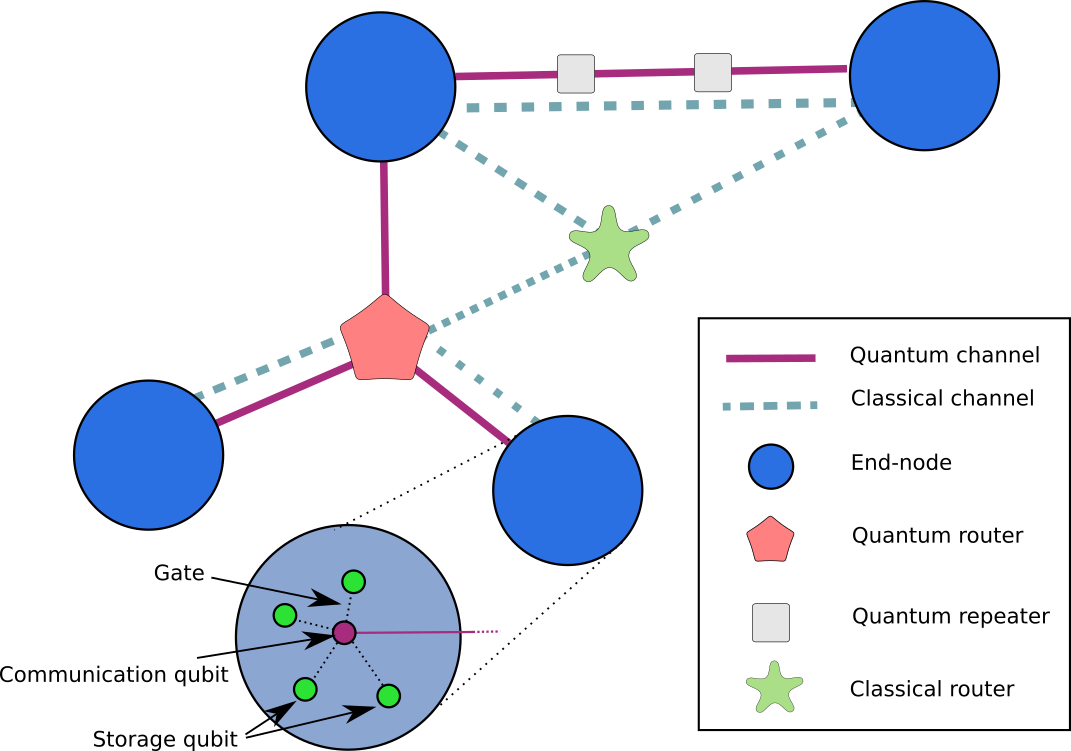
\includegraphics[width=0.4\linewidth]{figures/netqasm/network_model.png}
    \includegraphics[width=0.8\linewidth]{figures/background/network_nodes.pdf}
    \caption{
        Schematic overview of a quantum network.
        A quantum network consists of nodes (yellow and grey circles) that are connected by classical and quantum communication channels (grey lines).
        Each node implements a physical layer (green boxes and lines) that enables entanglement generation between neighboring nodes.
        % The physical layer is the domain of the QDevice.
        Each node implements a network stack including a network layer (red boxes and lines, which may be subdivided into a separate link layer and a network layer~\cite{dahlberg_2019_egp, kozlowski_2019_towards}).
        This layer realizes long-distance entanglement creation between nodes, and may include protocols such as entanglement swapping and distillation.
        % As QNodeOS implements a network stack, it can also be deployed on intermediary nodes in the network, where e.g. entanglement distillation could be added to the protocol realizing the network layer service implemented by QNodeOS.
        \newline
        We emphasize that the focus of this work is to program and execute applications on the end nodes, i.e. enabling the application layer in networking terms.
        Only \emph{end nodes} (yellow circles) implement an additional application layer (blue boxes and line), which executes arbitrary user applications.
        From the perspective of this layer, end nodes are logically directly connected (blue line) and this layer is hence independent from implementations and protocols in the network layer, and is only dependent on the service  provided by the network layer.
        Logically directly connected means that the application layer relies on the service of the network layer to enable end-to-end entanglement generation between end nodes, and no longer needs to concern itself how the entanglement is generated.
        This abstraction is a key element enabled by a quantum network stack such as~\cite{dahlberg_2019_egp}, and exactly analogous to similar abstractions used in classical networking, where e.g. a web browser can be executed on a laptop independently of how the internet connection between the laptop and a web server is realized.
        % In the same way, QNodeOS can in fact operate also on end nodes separated by a large quantum network of the future, in which many intermediary nodes may lie on the path connecting the end nodes.
    }
    \label{background:fig:network_model}
\end{figure}

\subsection{Quantum end nodes}
As mentioned above, end nodes in a quantum network possess a quantum processor acting on quantum memory.
These processors differ from classical processors in a number of ways.
Firstly, quantum memory has limited lifetime, meaning that its quality degrades over time.
For example, quantum memories based on nitrogen-vacancy (NV) centers in diamond have impressively been optimized to achieve lifetimes in the order of seconds~\cite{Abobeih2018};
however, this is still very short compared to classical memories, which generally do not have a limited lifetime at all.
Therefore, the quality of program execution is time-sensitive.
Secondly, physical devices are prone to inaccuracies which lead to decreased quality of (quantum) computation.
For example, applying an operation (like a gate) on a qubit affects that qubit's quality.
We note that the two challenges mentioned so far are also inherent to non-network quantum processors.
Quantum \textit{network} processors have additional challenges:
    (1) the processor may have to act as a local computation unit and a network interface at the same time;
    for example, in NV centers, an electron spin qubit is used for generating entanglement with a remote node but is also needed to do local two-qubit gates,
    (2) remote-entanglement operations may not have a fixed time in which they complete, which makes scheduling and optimization more difficult.

Each quantum memory has a certain \textit{topology} that describes which operations can be applied on which (pair of) qubits.
Some of the qubits in a quantum memory may be used to generate an entangled state with another node.
These qubits are called \emph{communication qubits}~\cite{dahlberg2019linklayer}, in contrast to \emph{storage qubits} which can only directly interact with other qubits part of the same local node.
A storage qubit may however hold a state that is entangled with a qubit in another node: after remote entanglement generation using a communication qubit, the state in that local qubit could be transferred to one of the storage qubits, preserving the remote entanglement.
Some platforms only have a single communication qubit and multiple storage qubits~\cite{Bernien2014}, whereas others can have multiple communication qubits~\cite{Inlek2017}.
Quantum processors in general offer two types of qubits (see e.g.~\cite{dahlberg_2019_egp}): \emph{communication qubits} which can be used to generate entanglement with remote nodes next to other quantum operations, as well as \emph{storage qubits} which cannot be used to generate entanglement and only for implementing local quantum operations.
We remark that on near-term quantum processors, the types of operations also depends on the connectivity of the qubits.
That is, not all (pairs of) qubits may allow the same set of quantum operations to be performed on them.

\paragraph{Noise and decoherence}
Qubits are sensitive to \emph{decoherence} and have limited lifetimes.
Therefore, the timing and duration of operations (such as local gates or entanglement generation with another node) have an impact on the quality of quantum memory. Classical processors control the quantum hardware, and also perform classical computation.
Finally, classical links exist between nodes for sending classical messages.

Since end nodes can control their memory and entanglement generation, they can run arbitrary \textit{user programs}.
End nodes can both communicate classically and generate entanglement between each other, either directly or through repeaters and routers, (\cref{background:fig:network_model}). Nodes in the network other than end nodes, such as repeaters and routers, do not execute user programs; rather these run protocols that are part of some level in the
network stack~\cite{dahlberg2019linklayer,kozlowski2020networklayer}.
These internal nodes in the network perform elementary link generation and entanglement swapping in order to generate long-distance remote entanglement between end nodes~\cite{dahlberg2019linklayer}.

\paragraph{Hardware implementations}
There are various quantum hardware implementations for quantum network processors, such as nitrogen-vacancy centers in diamond~\cite{Bernien2014}, ion traps~\cite{moehring2007entanglement}, and neutral atoms~\cite{hofmann2012heralded,ritter2012elementary}, which all have different capabilities and gates that can be performed.

\subsection{Quantum processing}
Quantum computing consists of performing operations on quantum bits (qubits).

\paragraph{Circuits and gates}
A quantum program is typically represented as a \emph{quantum circuit}.
\Cref{background:fig:example_circuit} shows an example circuit of 2 qubits.

\begin{figure}[t]
    \centering
    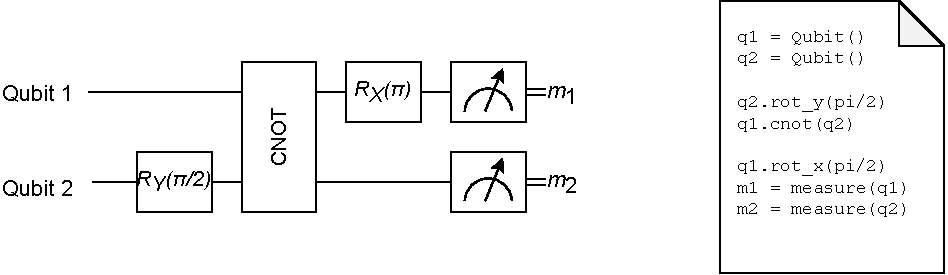
\includegraphics[width=0.8\linewidth]{figures/background/local_circuit.pdf}
    \caption{
        Two representations of an example quantum application using two qubits.
        This program can run on a quantum computer, which may be a node in a quantum network.
        Left: circuit model of the program.
        A horizontal line represents a single qubit.
        Blocks are quantum gates applied on qubits; there are single-qubit gates (such as a rotation gate around axis $X$ with angle $\pi$ (\texttt{R\_X(pi)})) and multi-qubit gates (such as a CNOT; note that a CNOT gate is also sometimes depicted as a vertical line and an XOR symbol on one of the qubits).
        Time goes from left to right, so the gates are applied in the order (left to right) they are depicted.
        A measurement `gate' destroys the qubit and produces a classical bit, depicted by a double line.
        Right: the same program but represented in a programming language (language shown is fictional and for illustration purposes only; in \cref{chp:netqasm} we present a real, detailed language).
        This is what a developer might write when programming (`coding') the program.
    }
    \label{background:fig:local_circuit}
\end{figure}



A quantum circuit describes the operations that are to be performed on the quantum memory consisting of individual qubits.
Operations include quantum gates (rotation gates or Hadamard), initialization, and measurement (readout).
Quantum gates may be on a single qubit, or on multiple qubits.
For example, the CNOT gate is a 2-qubit gate.

The code, or the `recipe` of quantum programs is hence classical.
The information and memory that the program manipulates is quantum.
Besides quantum operations, there may be limited classical control, such as a gate being executed depending on a measurement outcome.
Typically, a quantum circuit is executed in one go, on a very small timescale.
Quantum memory used for quantum computing~\cite{de_leon_materials_2021} often only stays coherent (alive and useful) for microseconds.

\paragraph{Hybrid classical-quantum processing}
Hybrid classical-quantum programs are used to realize e.g. \textit{variational quantum eigensolvers (VQE)}~\cite{diadamo2021distributed, liu2022layer} or \textit{quantum approximate optimization algorithms (QAOA)}~\cite{farhi2014quantum}.
For such programs, a quantum circuit is executed, followed by some classical processing, and a next circuit is issued.

\subsection{Entanglement generation}
In order for two neighboring quantum network nodes to produce heralded entanglement between them, they need to simultaneously perform an action to trigger entanglement generation (at the physical layer, \emph{synchronized to nanosecond precision}).
This means neighboring quantum network nodes need to perform a network operation (entanglement generation) in a \emph{very specific} time slot in which they make an attempt to generate entanglement.
Such time slots are generally aggregated into larger time bins, corresponding to making batches of attempts in time slots synchronized at the physical layer.
We refer to e.g. Ref.~\cite{pompili_2022_experimental} for background information on the physical layer of entanglement generation in quantum networks, and the readers with a background in computer science to e.g. Ref.~\cite{dahlberg_2019_egp} for a detailed explanation of scheduling of entanglement generation in quantum networks.

In short, network operations in quantum networks need to be executed by the node at very specific time bins.
These time bins cannot be determined by the quantum node itself.
Instead selection of time bins for a specific quantum operation require agreement with the neighboring node~\cite{dahlberg_2019_egp} (and more generally with the quantum network when the end-to-end entanglement is made via intermediary network nodes) by means of a network schedule, e.g. determined by a (logically) centralized controller, see Ref.~\cite{skrzypczyk_2021_arch}.

\paragraph{Quantum network stack}
A quantum network stack has been proposed~\cite{dahlberg2019link} and implemented~\cite{pompili2022experimental} that turns entanglement generation into a robust service independent of the quantum hardware platform.
Important for the design of an architecture for the execution of quantum internet applications is that in this stack, the nodes will establish a network schedule of time slots in which they will trigger entanglement generation (due to need to synchronize entanglement generation at the physical layer~\cite{dahlberg2019link} at high-precision (ns)).
This means that once entanglement has been requested from the network, the nodes can use only the slots in the network schedule to produce entanglement between them, imposing constraints on the ability to schedule applications. What's more, in present day systems~\cite{pompili2021realization, krutyanskiy2023entanglement} limitations in the physical devices prohibit the execution of local operations while engaging in network operations (entanglement generation), creating further dependencies between the local quantum execution and entanglement generation. 
As the specifics of network scheduling~\cite{network-scheduling, skrzypczyk2021architecture} are not within scope of this thesis,
we assume the existence of a \textit{network controller} that takes application demand for entanglement and issues a network schedule to the nodes. 
A schedule consists of sequential time slots, each with a start time and duration, when the node will trigger entanglement generation.
Nodes are not forced to attempt entanglement in corresponding time slots, and can instead choose to do local processing instead.


\begin{figure}[t]
    \centering
    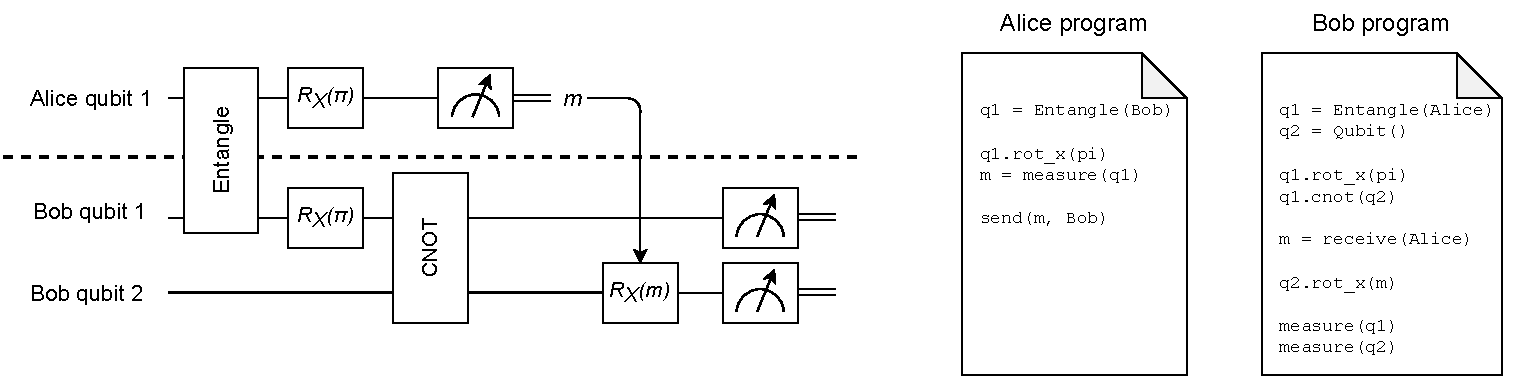
\includegraphics[width=1.0\linewidth]{figures/background/2node_circuit.pdf}
    \caption{
        Two representations of an example two-node quantum network application.
        The application is run on the nodes Alice (possessing one qubit) and Bob (possessing two qubits).
        Left: circuit model of the application.
        The Entangle operation is depicted here as a two-qubit gate; however since it acts on qubits in different nodes (Alice and Bob),
        this is not as trivial as a local two-qubit gate such as the CNOT.
        Furthermore, classical communication may happen in the form of sending a message.
        In this case, after measuring her qubit, Alice sends the classical outcome bit $m$ to Bob.
        Bob then uses this in his local X-rotation gate.
        Right: the same program but represented in a programming language.
        Since Alice and Bob are separated nodes, they each program their own local code.
        This code may however include external operations, such as entanglement creation with the other node, and sending or receiving messages.
        Note that these operations must match --- something they are responsible for themselves, by e.g. following some pre-established protocol.
    }
    \label{background:fig:2node_circuit}
\end{figure}

\section{Quantum network applications}
Quantum network \textit{applications}, also called \textit{protocols}, are multi-partite programs that involve entanglement generation and classical communication between different end nodes, as well as local computation.
Examples include Quantum Key Distribution (QKD)~\cite{bb84, ekert_1991_e91}, leader election protocols~\cite{kobayashi2014simpler, ganz2009quantum}, and Blind Quantum Computation (BQC)~\cite{Wehner2018stages}.
In this thesis, we consider quantum network applications in the quantum memory stage~\cite{wehner_2018_stages} and above. That is, applications that require the use of a quantum processor that can manipulate and store quantum bits (qubits). For simpler applications in the prepare-and-measure and entanglement generation stages~\cite{wehner_2018_stages}, e.g. quantum key distribution~\cite{bb84Original,ekert_1991_e91}, where the quantum states are immediately measured by the nodes, it would be sufficient to realize a system implementing a quantum network stack and classical processing only.


\subsection{Programs}
Throughout this thesis, we will use the following terminology.
Applications refer to multi-node protocols or use-cases of quantum networks, such as QKD, BQC, etc.
Programs refer to the code that is run on individual quantum network nodes.
Applications are realized by the joint execution of programs on their respective nodes.

A multi-node quantum internet application is hence partitioned into separate single-node \textit{programs} (e.g. a client program and a server program in BQC) that run concurrently on different network end nodes.
To support security sensitive applications, each program performs local classical and quantum computations on its own private node, and programs interact with each other only via classical message passing and entanglement generation.
This is in sharp contrast to distributed quantum computing (see e.g.~\cite{cacciapuoti2019quantum}), where all nodes can be accessed and controlled by a single program. 


Such applications are split into distinct \textit{programs} each of which runs on a separate end node.


\paragraph{Program ingredients}
% unit of information: bit vs qubit}
% unit of instruction still classical in quantum computing

The single-node programs that constitute a quantum internet application are hybrid in nature (see Fig~\ref{fig:program_illustration}):
First, they contain quantum operations, such as local quantum gates and measurements (e.g. to perform a server computation in BQC), and entanglement generation (e.g. to produce key in QKD). Entanglement is a special property of two quantum bits (qubits) that forms a key resource for quantum internet applications. 
All quantum operations are executed on quantum processors that can store, manipulate and measure quantum information, where small networks including such processors have been realized using different quantum hardware platforms including, for example,  Nitrogen-Vacancy (NV) centers in diamond~\cite{pompili2021realization}, and Ion Traps~\cite{krutyanskiy2023entanglement}.
Second, programs need to perform classical operations, such as message passing (e.g., a BQC client program sending desired measurement bases to the BQC server), and local classical processing (e.g., post-processing measurement outcomes in QKD).


A program is a series of instructions to be executed by a node.
Instructions can be categorized into four types: local classical processing, classical message-passing, quantum local processing (quantum operations), and remote entanglement generation.
A program can keep classical variables in a classical memory, and quantum variables (qubits) in the node's quantum memory during the execution.
Multiple programs, each running on their own node, together form an \textit{application} (see~\ref{fig:program_illustration}), e.g. QKD (two programs, one per node),
or secret sharing~\cite{hillery1999quantum} (a program each on many nodes).
Programs may involve asynchronous operations (e.g. a server awaiting entanglement with multiple clients).


Classical blocks of code consist of instructions for local classical operations and classical message passing. Quantum \emph{blocks of code} consists of
%
\begin{inlinelist}
\item quantum operations (initialization, quantum gates, measurement), 
\item low-level classical control logic (branching on classical variables and loops), as well as 
\item instructions to make entanglement between remote nodes. 
\end{inlinelist}
%

\paragraph{Interactivity}
Classical blocks of code may depend on quantum ones via classical variables generated during the quantum execution (such as measurement results, notification of entanglement generation, and information on the state of the quantum system such as the availability of qubits).
Similarly, quantum blocks may depend on variables set by the classical blocks (such as messages received from remote network nodes).
Finally, quantum blocks may themselves depend on other quantum blocks via qubits in the quantum memory. 

The programs consist of both local operations (classical and quantum) and network operations (classical and quantum), see \cref{fig:app_programs}.
That is, the programs communicate either by passing classical messages, or by establishing quantum entanglement.
For example, BQC involves a \textit{client} node and a \textit{server} node, both of which run their own program.
Their joint execution looks roughly as follows:
    (1) The client and server engage in remote entanglement generation such that the server's quantum memory ends up being in a certain state,
    (2) the client sends instructions to the server in the form of a classical message,
    (3) the server performs a measurement-based computation on its own quantum memory based on the client's instructions,
    (4) the server sends measurement results back to the client,
    (5) the client sends new instructions based on the measurement results,
    (6) repeat steps 3 to 5 until the client obtains its desired result.

The example above illustrates that quantum network programs consist of different
types of operations.
Indeed, program code consists of \textit{classical code}, containing local classical operations and classical communication with other nodes, and \textit{quantum code}, which are operations on quantum memory (such as \textit{gates}) and remote entanglement generation.
Blocks of these types of code may depend on each other in multiple ways, as depicted in~\cref{fig:program_decomp}.
Programs with mixed classical and quantum operations have also been called \textit{dynamic quantum circuits}~\cite{cross2021openqasm, burgholzer2021towards}, but these do not cover the networking dimension found in programs we consider here, such as the dependency on remote information and entanglement generation operations.

Due to the nature of quantum network programs, execution may have to \textit{wait} for some time. For example, the program needs to wait until another node sends a classical message, or until remote entanglement has been established.
Therefore, it makes sense to run multiple (independent) quantum network programs on a node at the same time (interleaved), so that processor idle times can be filled by execution of other programs. This is something that typically does not happen on local quantum computers, and therefore introduces new challenges.

\paragraph{Independence of programs}
Quantum network applications may be programmed by a single actor.
For example, a developer may program a QKD application in the form of a two programs, and distribute these two programs to two end nodes in the network.
Alternatively, a single-node quantum network program may be developed separately from other programs, possibly not knowing how these other programs are implemented.
For example, a BQC service provider could have already implemented the server-side program of a specific BQC protocol.
A client may then write the client-side of this protocol, without having control over the server-side implementation.



\subsection{Application execution}

\paragraph{Mode of Execution}
There exist quantum applications and functionalities, where one pair of programs is executed only once, e.g. a simple example of quantum teleportation~\cite{bennett_1993_teleportation}.
As in quantum computing, however, some quantum network applications~\cite{wehner_2018_stages} are expected to succeed only with a specific \emph{probability of success} $p_{\rm succ}$ when executed once.
In many quantum internet applications (e.g. BQC), a single execution of the application can result in failure or success (e.g. a BQC client receives correct measurement results from the server program~\cite{leichtle2021verifying}).
Quantum internet applications have classical outcomes that are typically probabilistic in nature:
(1) applications may intentionally do measurements on quantum states that have fundamentally probabilistic outcomes (e.g. quantum cryptography),
(2) in practice, quantum hardware is imperfect (or \textit{noisy}). That is, undesired errors occur
when performing operations (such as gates, measurements, or entanglement generation) or when keeping quantum states in memory for too long.
Applications are often executed many times, where outcome statistics are computed in order to validate successful execution (e.g. by majority of outcomes).
The application is then typically executed many times in succession in order to gather statistics (for example to amplify $p_{\rm succ}$).


\paragraph{Performance metrics}
Performance of application execution on quantum network nodes can be measured by several metrics.
In this thesis we consider metrics that either apply to a single application that one executes on the quantum network, or on a node in the network that executes one or more applications.

For an application, we consider \textit{makespan} as a classical metric and \textit{success probability} as a quantum metric.
Makespan is the time it takes to execute (all repetitions of) the application.
The success probability is the one mentioned above.
It is typically related to quantum fidelity $F \in [0, 1]$, which is a measure of closeness of a quantum state to some ideal quantum state.
Noisy quantum systems produce non-perfect quantum states ($F < 1$) which decrease application success probability.
For quantum network nodes, we consider common classical metrics~\cite{stankiewicz_commag}: utility (fraction of time that a node is doing useful things), throughput (amount of application executions per time unit) and latency (which may be between internal components of a node, or between nodes).




\begin{xstretch}
\printbibliography[heading=subbibintoc,title={References},notcategory=noprint]
\end{xstretch}

\chapter
 [NetQASM: A low-level instruction set architecture for hybrid quantum-classical programs in a quantum internet]
 {NetQASM: A low-level instruction set architecture for hybrid quantum-classical programs in a quantum internet}
\label{chp:netqasm}

\newcommand{\netqasm}{\texttt{NetQASM}}
\newcommand{\qasm}{\texttt{QASM}}
\newcommand{\openqasm}{\texttt{OpenQASM}}
\newcommand{\cqc}{\texttt{CQC}}
\newcommand{\qnodeos}{\texttt{QNodeOS}}
\newcommand{\qdevice}{\texttt{QDevice}}
% \newcommand{\host}{\texttt{Host}}
\newcommand{\host}{application layer}
\newcommand{\QNPU}{\texttt{QNPU}}
\newcommand{\netsquid}{\texttt{NetSquid}}
\newcommand{\squidasm}{\texttt{SquidASM}}
\newcommand{\simulaqron}{\texttt{SimulaQron}}
\newcommand{\IMMEDIATE}{\textbf{IMMEDIATE}}
\newcommand{\REGISTER}{\textbf{REGISTER}}
\newcommand{\ADDRESS}{\textbf{ADDRESS}}
\newcommand{\ARRAYENTRY}{\textbf{ARRAY\_ENTRY}}
\newcommand{\ARRAYSLICE}{\textbf{ARRAY\_SLICE}}


\begin{abstract}
    We introduce NetQASM, a low-level instruction set architecture for quantum
    internet applications. NetQASM is a universal, platform-independent and
    extendable instruction set with support for local quantum gates, powerful
    classical logic and quantum networking operations for remote entanglement
    generation. Furthermore, NetQASM allows for close integration of classical
    logic and communication at the application layer with quantum operations at
    the physical layer. This enables quantum network applications to be
    programmed in high-level platform-independent software, which is not
    possible using any other QASM variants. We implement NetQASM in a series of
    tools to write, parse, encode and run NetQASM code, which are available
    online. Our tools include a higher-level SDK in Python, which allows an easy
    way of programming applications for a quantum internet. Our SDK can be used
    at home by making use of our existing quantum simulators, NetSquid and
    SimulaQron, and will also provide a public interface to hardware released on
    a future iteration of Quantum Network Explorer.
\end{abstract}

\blfootnote{
This chapter is extracted from the article:
\fullcite{dahlberg_2022_netqasm}.

Contributions: TODO
}

\newpage

\section{Introduction}
\label{sec:introduction}
\dropcap{Q}uantum mechanics shows that if one is able to communicate quantum information between nodes in a network, one is able to achieve certain tasks which are impossible using only classical communication.
There are many applications~\cite{Wehner2018stages} where a \emph{quantum network} has advantage over a \emph{classical (non-quantum) network}, either by
    (1) enabling something that is theoretically impossible in a classical network, such as the establishment of an unconditionally secure key~\cite{bb84} and secure blind quantum computing~\cite{childs2005assisted} or
    (2) allowing something to be done faster or more efficiently such as exponential savings in communication~\cite{Buhrman2010} and extending the baseline of telescopes~\cite{gottesman2012longer}.
In recent years, many experiments have been conducted to show that a quantum network is not only a theoretical concept, and indeed advancements have been made to implement such a quantum network on various hardware platforms.
\cite{Hensen2015, Humphreys2018, moehring2007entanglement, hofmann2012heralded, Kalb2017, Inlek2017, sangouard2011quantum}.
However, these experiments alone do not yet make a quantum network \textit{programmable}, since the program logic was hard-coded into the experimental hardware ahead of time.
\footnote{There have been examples of experiments with some simple logic but only with a very limited number of pre-loaded decision-branches.}

Before considering how to program quantum network applications, let us first briefly sketch the system our applications are run on.
Abstractly, quantum networks consist of \textit{nodes} that are connected by \textit{channels} (\cref{fig:network_model}).
Classical channels enable classical communication between nodes, while quantum channels are used for \textit{entanglement} generation between nodes.
So-called \textit{end-nodes} may contain \textit{quantum processors} that can run arbitrary (quantum) programs.
They have access to a quantum memory consisting of qubits, on which they can perform operations, including quantum computations.
Some of these qubits may be used for establishing an entangled quantum state with a remote node.
An end-node also possesses a classical processor and a classical memory.
Furthermore, an end-node can send and receive classical messages to and from other end-nodes in the network.
A network of quantum networks may be a called a \textit{quantum internet}.

Quantum (network) processors differ from classical processors in a number of ways.
Firstly, quantum memory has limited lifetime, meaning that its quality degrades over time.
For example, quantum memories based on nitrogen-vacancy (NV) centers in diamond have impressively been optimized to achieve lifetimes in the order of seconds~\cite{Abobeih2018};
however, this is still very short compared to classical memories, which generally do not have a limited lifetime at all.
Therefore, the quality of program execution is time-sensitive.
Secondly, physical devices are prone to inaccuracies which lead to decreased quality of (quantum) computation.
For example, applying an operation (like a gate) on a qubit affects that qubit's quality.
We note that the two challenges mentioned so far are also inherent to non-network quantum processors.
Quantum \textit{network} processors have additional challenges:
    (1) the processor may have to act as a local computation unit and a network interface at the same time;
    for example, in NV centers, an electron spin qubit is used for generating entanglement with a remote node but is also needed to do local two-qubit gates,
    (2) remote-entanglement operations may not have a fixed time in which they complete, which makes scheduling and optimization more difficult.

Quantum network \textit{applications}, also called \textit{protocols}, are multi-partite programs that involve entanglement generation and classical communication between different end-nodes, as well as local computation.
Examples include Quantum Key Distribution (QKD)~\cite{bb84, ekert1991quantum}, leader election protocols~\cite{kobayashi2014simpler, ganz2009quantum}, and Blind Quantum Computation (BQC)~\cite{Wehner2018stages}.
Such applications are split into distinct \textit{programs} each of which runs on a separate end-node.
The programs consist of both local operations (classical and quantum) and network operations (classical and quantum), see \cref{fig:app_programs}.
That is, the programs communicate either by passing classical messages, or by establishing quantum entanglement.
For example, BQC involves a \textit{client} node and a \textit{server} node, both of which run their own program.
Their joint execution looks roughly as follows:
    (1) The client and server engage in remote entanglement generation such that the server's quantum memory ends up being in a certain state,
    (2) the client sends instructions to the server in the form of a classical message,
    (3) the server performs a measurement-based computation on its own quantum memory based on the client's instructions,
    (4) the server sends measurement results back to the client,
    (5) the client sends new instructions based on the measurement results,
    (6) repeat steps 3 to 5 until the client obtains its desired result.

The example above illustrates that quantum network programs consist of different
types of operations.
Indeed, program code consists of \textit{classical code}, containing local classical operations and classical communication with other nodes, and \textit{quantum code}, which are operations on quantum memory (such as \textit{gates}) and remote entanglement generation.
Blocks of these types of code may depend on each other in multiple ways, as depicted in~\cref{fig:program_decomp}.
Programs with mixed classical and quantum operations have also been called \textit{dynamic quantum circuits}~\cite{cross2021openqasm, burgholzer2021towards}, but these do not cover the networking dimension found in programs we consider here, such as the dependency on remote information and entanglement generation operations.

Due to the nature of quantum network programs, execution may have to \textit{wait} for some time. For example, the program needs to wait until another node sends a classical message, or until remote entanglement has been established.
Therefore, it makes sense to run multiple (independent) quantum network programs on a node at the same time (interleaved), so that processor idle times can be filled by execution of other programs. This is something that typically does not happen on local quantum computers, and therefore introduces new challenges.

Quantum network applications may be programmed by a single actor.
For example, a developer may program a QKD application in the form of a two programs, and distribute these two programs to two end-nodes in the network.
Alternatively, a single-node quantum network program may be developed separately from other programs, possibly not knowing how these other programs are implemented.
For example, a BQC service provider could have already implemented the server-side program of a specific BQC protocol.
A client may then write the client-side of this protocol, without having control over the server-side implementation.

The aim of this work is to propose a way to program quantum network programs and execute them on the end-nodes of a quantum network.


\begin{figure}[h]
    \centering
    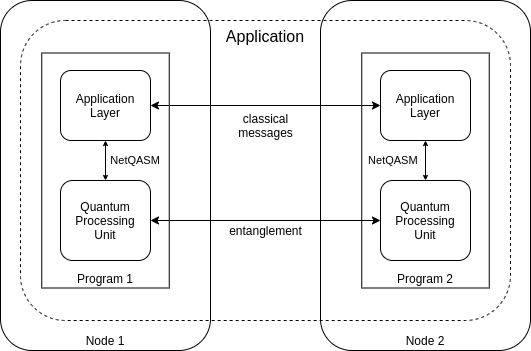
\includegraphics[width=0.6\textwidth]{figures/netqasm/multi_program_app_2.png}
    \caption{A quantum network application consists of a program for each of the nodes involved in the application.
        Each program is locally executed by the node.
        Program execution on each node is split into execution in an application layer, which can send and receive classical messages, and a quantum processor, which can create entanglement with another node.
        The communication between nodes can hence be both classical and quantum.
        Communication instructions need to be matched by corresponding instructions in the other program.
        There is no global actor overseeing execution of each of the programs, and the nodes may be physically far apart.}
    \label{fig:app_programs}
\end{figure}

\begin{figure}[h]
    \centering
    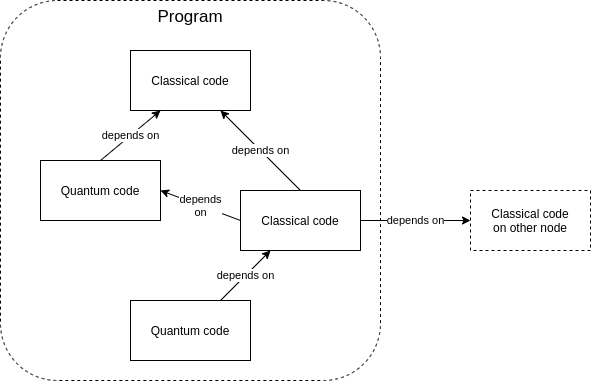
\includegraphics[width=0.6\textwidth]{figures/netqasm/program_decomp.png}
    \caption{A program on a single node consists of different blocks of code, which can be quantum (pure quantum instructions with classical control in between), or classical (no quantum operations at all).
        These blocks may depend on each other in various ways.
        For example, the outcome of a measurement happening in one of the quantum blocks may be used in a calculation performed in one of the classical blocks.
        Blocks may also depend on other nodes.
        For instance, the value of a message coming from another node can influence the branch taken in one of the classical blocks.}
    \label{fig:program_decomp}
\end{figure}


\subsection{Contribution}
In this work we introduce an abstract model---including a quantum network processing unit (\QNPU)--- for end-nodes in a quantum network, which we define in~\cref{sec:preliminaries}.
We then propose \netqasm, an instruction set architecture that can be used to run arbitrary programs (of the form described in \cref{fig:program_decomp}) on end-nodes, as long as the end-nodes realize the model including the QNPU.

\netqasm consists of a specification of a low-level assembly-like language to express the quantum parts of quantum network program code.
It also specifies how the application layer should interact with the \QNPU and how the assembly language can be used to execute (network) quantum code.
This is not possible using other \qasm languages.

The \netqasm language is extendible using the concept of \textit{flavors}.
The core language definition consists of a common set of instructions that are shared by all flavors.
This common set contains classical instructions for control-flow and classical memory operations.
This allows the realization of low-level control logic close to the quantum hardware;
for example, to perform branching based on a measurement outcome.
Quantum-specific instructions are bundled in flavors.
We introduce a \textit{vanilla} flavor containing universal platform-independent quantum gates.
Using this flavor of the \netqasm language enables the platform-independent description of quantum network programs.
Platform-\textit{specific} flavors may be created to have quantum operations that are native and optimized for a specific hardware platform.
As an example, we show a flavor tailored to the Nitrogen-Vacancy (NV) hardware, a promising platform for quantum network end-nodes~\cite{Taminiau2014, hanson2021realization}.

In our model, application-specific classical communication only happens at the application layer (\cref{fig:app_programs}).
In particular, this means that \netqasm contains no provision for classical communication with the remote node.
We remark that of course, classical control communication may be used by the \QNPU to realize the services of the quantum network stack accessed through \netqasm.

We note that \netqasm is used for representing and running code that runs on a single node in a quantum network.
Synchronization between the (\netqasm) programs of multiple nodes is the responsibility of the programmer.
For example, in a client-server application, if the client code contains a `receive classical message' operation, it is the responsibility of the server node that its program code contains a `send classical message' operation at the right moment.
The same holds for instructions for creating remote entanglement.
In terms of precise timing, which is needed for entanglement generation, it is the \QNPU that is responsible to communicate and synchronize with the \QNPU of the other node to make sure entanglement attempts are synchronized.

With \netqasm\, we solve various problems that are unique to quantum internet programming:
    (1) for remote entanglement generation, we introduce new instruction types for making use of an underlying quantum network stack~\cite{dahlberg2019linklayer, kozlowski2020networklayer},
    (2) for the close interaction between classical and quantum operations, we use a shared-memory model for sharing classical data between the application layer and the \QNPU,
    (3) in order to run multiple applications on the same quantum node---which may be beneficial for overall resource usage (see~\cref{sec:design_considerations})---we make use of virtualized quantum memory, similar to virtual memory in classical computing~\cite{arpaci2018operating},
    (4) since on some platforms, not all qubits may be used to generate remote entanglement, we introduce the concept of unit-modules describing qubit topologies with additional information per (virtual) qubit about which operations are possible.

Since \netqasm\ is meant to be low-level, similar in nature to classical assembly languages, we have also developed a higher-level software development kit (SDK), in Python, to make it easier to write applications.
This SDK and related tools are open-source and freely available at~\cite{git_netqasm}, as part of our Quantum Network Explorer~\cite{qne_website}.
Through the SDK we have also enabled the quantum network simulators \netsquid~\cite{coopmans2021netsquid} and \simulaqron~\cite{dahlberg2018simulaqron} to run any application programmed in \netqasm.

We have evaluated \netqasm\ by simulating the execution of a teleportation application and a blind quantum computation using \netqasm.
Hereby we have shown that interesting quantum internet applications can indeed be programmed using \netqasm.
Furthermore, the evaluations argue certain design choices of \netqasm, namely the use of so-called \textit{unit modules}, as well as platform-specific
\textit{flavors}.

We remark that \netqasm has already been used on a real hardware setup in the lab, in a highly simplified test case that only produces entanglement~\cite{pompili2021experimental}.

\subsection{Related Work}
\label{sec:related}
In the field of quantum computing, a substantial amount of progress has been made related to developing
architectures (e.g.~\cite{fu2017microarchitecture,bourassa2020photonicblueprint, murali2019fullstack, wecker2014liqui, khammassi2020openql, amy2019staq, green2013quipper, Steiger2016}),
instruction sets (e.g.~\cite{cross2017openqasm,khammassi2018cqasm,fu2019eqasm,liu2017fqasm,smith2016quil,qiskit,cirq,qsharp,jones2019quest}) and
compilers~\cite{zulehner2019compiling, haner2018software, gokhale2020quantum, liu2020new, gokhale2020optimized, ding2020square, smith2020opensource, Sivarajah_2020, hietala2019verified, zhang2020contextmapping, niu2020hardware, dury2020qubo, pozzi2020using, Nishio_2020}.
One example is \qasm, an instruction set framework, borrowing ideas from classical assembly languages, which has gained a lot of popularity over the years and has been successfully integrated in software stacks for quantum computers.
There are in fact many variants of \qasm such as \openqasm~\cite{cross2017openqasm}, \texttt{cQASM}~\cite{khammassi2018cqasm}, \texttt{eQASM}~\cite{fu2019eqasm}, \texttt{f-QASM}~\cite{liu2017fqasm}.
Some of these variants are at a level closer to the physical implementation, such as \texttt{eQASM}, allowing for specifying low-level timing of quantum operations, while others, such as \texttt{f-QASM}, are at a higher level.
Together with the definition of these \qasm-variants, progress has also been made in compilation of applications programmed in \qasm\ to hardware implementations.
More abstract languages and programming frameworks for quantum programs include \texttt{Quil}~\cite{smith2016quil}, \texttt{Qiskit}~\cite{qiskit}, \texttt{Cirq}~\cite{cirq}, \texttt{Q\#}~\cite{qsharp}, \texttt{QuEST}~\cite{jones2019quest}.

None of these instruction sets or languages contain elements for remote entanglement generation (i.e. between different nodes), which \netqasm does provide.
A \netqasm program that uses the vanilla flavor and only contains local operations would look similar to an \openqasm program.
However, the instruction set is not quite the same, since \netqasm uses a different memory model than \openqasm.
This is due to the hybrid nature of quantum network programs, which has more interaction between classical data and quantum data than non-networking programs (for which \openqasm might be used).
So, \netqasm is not just a superset of the \openqasm instruction set (in the sense of adding entanglement instructions).

In~\cite{dahlberg2018simulaqron}, we introduced the \cqc interface, which was a first step towards a universal instruction set.
However, \cqc had a number of drawbacks, in particular:
    (1) \cqc does not have a notion of virtualized memory (see \cref{sec:design_considerations}), which meant that applications needed to use qubit IDs that were explicitly provided by the underlying hardware.
        This introduced more communication overhead and fewer optimization opportunities for the compiler.
    (2) \cqc does not provide as much information about hardware details.
        Therefore, platform-specific compilation and optimization is not possible.
    (3) Furthermore, \cqc does not match entirely with the later definition of our quantum network stack~\cite{dahlberg2019linklayer, kozlowski2020networklayer}.
        For example, it was not clearly defined how \cqc relates to the definition of a network layer.

Many of the ideas from e.g. \qasm\ for how to handle and compile local gates can be reused also for quantum network applications.
For example, version 3 of \openqasm~\cite{cross2021openqasm} which is under development, proposes close integration between \emph{local} classical logic and quantum operations, which is something we also propose in this work.
However, there are two key differences that we need to address:
\begin{enumerate}
      \item Instructions for generating entanglement between remote nodes in the network need to be handled and integrated with the rest of the application, see \cref{sec:abstract_model} below.
      \item The local operations performed by a node might depend on information communicated by another node and only known at runtime.
            Note that this is different from the conditionals on \emph{local} classical information, proposed in for example \openqasm version 3, which does not require communication between remote nodes in a network.
            This brings new constraints in how to handle memory allocation, scheduling and addressing.
            We discuss this point in further detail in the coming sections.
\end{enumerate}
\netqasm\ solves the above two points and improves upon \cqc.


\subsection{Outline}
In \cref{sec:preliminaries} we define relevant concepts and introduce the model of end-nodes that we use, including the \QNPU.
In \cref{sec:use_cases} we discuss use-cases of a quantum network which \netqasm\ should support.
In \cref{sec:design_considerations} we consider requirements and considerations any instruction set architecture for quantum networks should fulfill which then lay the basis for the decisions that went into developing \netqasm, see \cref{sec:design_decisions}.
In \cref{sec:implementation} and \cref{sec:python-sdk} we describe details about the \netqasm\ language and associated SDK.
In \cref{sec:evaluation} we quantitatively evaluate some of the design decision of \netqasm\ by benchmarking quality of execution using the quantum network simulator \netsquid~\cite{netsquid,coopmans2021netsquid}.
We conclude in \cref{sec:conclusion}.


\section{Preliminaries and Definitions}\label{sec:preliminaries}

\subsection{Quantum networks}
\label{sec:quantum_networks}
A schematic overview of quantum networks is given in~\cref{fig:network_model}.
A quantum network consists of \textit{end-nodes} (hereafter also: \textit{nodes}), which contain quantum network processors as well as classical processors.
Nodes are connected by \textit{quantum channels} or \textit{links} that can be used to generate \textit{entangled} quantum states across nodes.
End-nodes possess quantum memory in the form of qubits, which can be manipulated by performing \textit{operations} such as initialization, readout, and single- or multi-qubit \textit{gates}.
Each quantum memory has a certain \textit{topology} that describes which operations can be applied on which (pair of) qubits.
Some of the qubits in a quantum memory may be used to generate an entangled state with another node.
These qubits are called \emph{communication qubits}~\cite{dahlberg2019linklayer}, in contrast to \emph{storage qubits} which can only directly interact with other qubits part of the same local node
\footnote{A storage qubit may however hold a state that is entangled with a qubit in another node: after remote entanglement generation using a communication qubit, the state in that local qubit could be transferred to one of the storage qubits, preserving the remote entanglement.}.

Some platforms only have a single communication qubit and multiple storage qubits~\cite{Bernien2014}, whereas others can have multiple communication qubits~\cite{Inlek2017}.
Qubits are sensitive to \textit{decoherence} and have limited lifetimes.
Therefore, the timing and duration of operations (such as local gates or entanglement generation with another node) have an impact on the quality of quantum memory. Classical processors control the quantum hardware, and also perform classical computation.
Finally, classical links exist between nodes for sending classical messages.

Since end-nodes can control their memory and entanglement generation, they can run arbitrary \textit{user programs}.
End-nodes can both communicate classically and generate entanglement between each other, either directly or through repeaters and routers, (\cref{fig:network_model}). Nodes in the network other than end-nodes, such as repeaters and routers, do not execute user programs; rather these run protocols that are part of some level in the
network stack~\cite{dahlberg2019linklayer,kozlowski2020networklayer}.
These internal nodes in the network perform elementary link generation and entanglement swapping in order to generate long-distance remote entanglement between end-nodes~\cite{dahlberg2019linklayer}.

There are various quantum hardware implementations for quantum network processors, such as nitrogen-vacancy centers in diamond~\cite{Bernien2014}, ion traps~\cite{moehring2007entanglement}, and neutral atoms~\cite{hofmann2012heralded,ritter2012elementary}, which all have different capabilities and gates that can be performed.

In contrast to classical networks, we consider the end-nodes in a quantum network to not have a network interface component that is separated from the main processing unit.
Having local and networking operations combined in a single interface reflects the physical constraint on current and near-term hardware.
Current state-of-the-art hardware for quantum networking devices can make use of up to the order of 10 qubits~\cite{bradley2019solidstate}.
Furthermore, certain hardware implementations, such as nitrogen-vacancy centers in diamond~\cite{Bernien2014}, only have a single communication qubit, which also acts as a mediator for any local gate on the storage qubits.
This prevents dedicating some qubits for purely local operations and some for purely networking operations.
Rather, to make maximal use of near-term quantum hardware, a multi-purpose approach needs to be supported.

\begin{figure}[h]
    \centering
    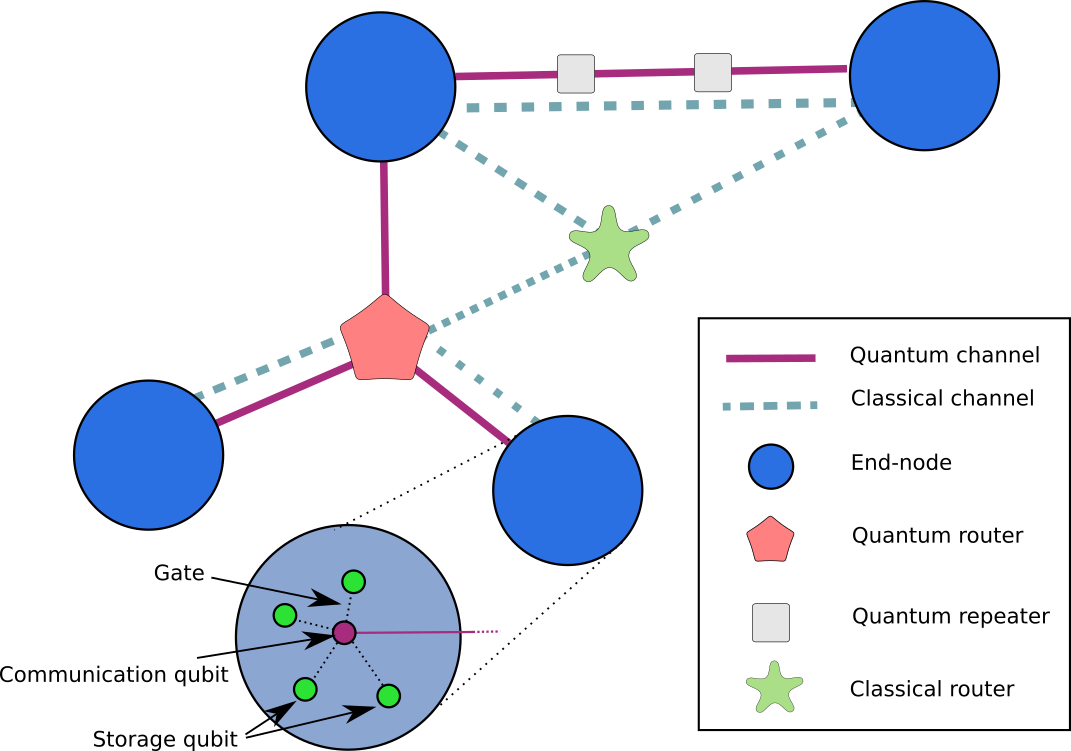
\includegraphics[width=0.7\textwidth]{figures/netqasm/network_model.png}
    \caption{Abstract model of a quantum network and its components. Quantum
        network applications run on the \emph{end-nodes} (blue). Their
        communication via classical message passing and quantum
        entanglement~(\cref{fig:app_programs}) is abstracted away by a network
        stack. That is, it is not visible at the application layer how
        entanglement generation or classical message passing is realized. This
        may be via direct physical connections, or intermediary repeaters and/or
        routers. End-nodes hold two types of qubits: (1) \emph{communication
            qubits} which can be used to generate entanglement with remote nodes and
        (2) \emph{storage qubits} which can be used to store quantum states and
        apply operations. A communication qubit may also be used as a storage
        qubit. The qubits within an end-node can interact through quantum gates
        and their state can be measured.}\label{fig:network_model}
\end{figure}



\subsection{Application layer and QNPU}
\label{sec:abstract_model}

In this work we will assume an abstract model of the hardware and software architecture of end-nodes in a quantum network.
Specifically, we assume each end-node to consist of an \host and a \emph{Quantum Network Processing Unit} (\QNPU).
The \host can be also be seen as a the user space of a classical computer, and the \QNPU as a coprocessor.

This model takes into account both physical- and application-level constraints found in quantum network programming.
The \QNPU\ can be accessed by the \host, at the same node, to execute quantum and classical instructions.
We define the capabilities of the \QNPU, and roughly their internal components, but do not assume how exactly this is implemented.
In the rest of this work, we simply use the \QNPU as a black box.

The \QNPU can do both classical and quantum operations, including
    (1) local operations such as classical arithmetic and quantum gates and
    (2) networking operations, i.e. remote entanglement generation.
The \host\ cannot do any quantum operations.
It can only do local computation and classical communication with other nodes.
In terms of classical processing power, the difference between the \host and the \QNPU is that the \host can do heavy and elaborate computation, while we assume the \QNPU to be limited in processing power.

The \host\ can interact with the \QNPU\ by for example sending instructions to do certain operations.
The \host\ and the \QNPU\ are logical components and may or may not be the same physical device.
It is assumed that there is low latency in the communication between these components, and in particular that they are physically part of the same node in the network.

One crucial difference between the \host and the \QNPU is that the \host can do application-level classical communication with other end-nodes, while the \QNPU cannot.
The \QNPU can communicate classically to synchronize remote entanglement generation, but it does not allow arbitrary user-code classical communication.
We use this restriction in order for the \QNPU to have relatively few resource requirements.

The \QNPU\ consists of the following components, see \cref{fig:qnpu}:
\begin{itemize}
    \item \textbf{Processor:}
            The processor controls the other components of the \QNPU\ and understands how to execute the operations specified by the \host.
            It can read and write data to the classical memory and use this data to make decisions on what operations to do next.
            It can apply quantum gates to the qubits in the quantum memory and measure them as well.
            Measurement outcomes can be stored in the classical memory.
    \item \textbf{Classical memory:}
            Random-access memory storing data produced during the execution of operations, such as counters, qubit measurement outcomes, information about generated entangled pairs, etc.
    \item \textbf{Quantum memory:}
            Consists of communication and storage qubits, see \cref{sec:quantum_networks}, on which quantum gates can be applied.
            The qubits can be measured and the resulting outcome stored in the classical memory by the processor.
            The communication qubits are connected through a quantum channel to adjacent nodes in the quantum network, through which they can be entangled.
            This quantum channel may also include classical communication needed for synchronization, phase stabilization or other mechanisms needed in the specific realization.
    \item \textbf{Quantum network stack:}
            Communicates classically with other nodes and quantum repeaters in the network to synchronize the generation of remote entanglement, and issues low-level instructions to execute the entanglement generation procedures, see~\cite{dahlberg2019linklayer,kozlowski2020networklayer}.
\end{itemize}

We stress that the internals of the \QNPU are not relevant to the design of \netqasm.
We do assume that the \QNPU only has limited classical processing power, and can therefore be implemented on for example a simple hardware board.


\begin{figure}
    \centering
    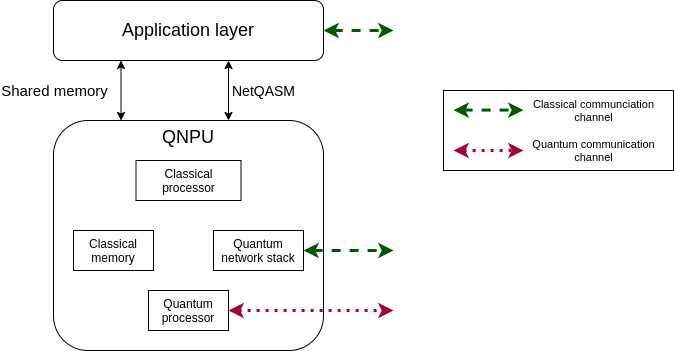
\includegraphics[width=0.8\textwidth]{figures/netqasm/qnpu.png}
    \caption{Overview of \QNPU\ components and interfaces. The \host\ talks to
        the \QNPU\ using \netqasm. The processor inside the \QNPU\ can interact with
        all other components. Channels are connecting components with corresponding
        components in adjacent nodes in the network.}
    \label{fig:qnpu}
\end{figure}



\subsection{Applications and programs}
As mentioned in~\cref{sec:introduction}, quantum network \textit{applications} (or protocols) are multi-partite and distributed over multiple end-nodes.
The unit of code that is executed on each of the end-nodes that are part of the application, is called a \textit{program}.
We will use this terminology throughout the rest of the paper.

As mentioned in the previous section, the end-nodes are modeled such that there is an application layer and a \QNPU. We assume that execution of quantum network programs is handled by the application layer.
How exactly the program is executed, and how the \QNPU is involved herein, is part of the \netqasm proposal.


\section{Use-cases}
\label{sec:use_cases}
In the next section we will discuss the design considerations taken when developing \netqasm.
These design considerations are based on a set of use-cases listed in this section which we intend for \netqasm\ to support.
Applications intended to run on a quantum network will often depend on a combination of these use-cases.

\begin{itemize}
      \item \textbf{Local quantum operations}.
            Applications running on a network node need to perform quantum operations on local qubits, including initialization, measurement, and single- or multi-qubit gates.
            Such local qubit manipulation is well known in the field of quantum computing. For example, \openqasm~\cite{cross2017openqasm} describes quantum operations.
            Quantum \textit{network} applications should be able to do these local operations as well.

      \item \textbf{Local quantum operations depending on local events or data}.
            The next use-case stems from applications consisting of programs in which limited classical computation or decision making is needed in-between performing quantum operations.
            Here we consider only dependencies in a program between quantum operations and information that is produced locally, that is, on the node that this program is being executed.
            For instance, a program might only apply a quantum gate on a qubit depending on the measurement outcome of another qubit, or choose between execution branches based on evaluation of a classical function of earlier measurement outcomes.
            An example is for the server-side of \textit{blind quantum computation}, which performs a form of Measurement-Based Quantum Computation (MBQC).
            In each step of the MBQC, the server performs certain gates on a qubit, depending on results of measuring previous qubits~\cite{fitzsimons2017private}.
            These applications need classical operations to not take too much time, so that qubit states stay coherent during these operations.
            This implies that switching between classical and quantum operations should have little overhead.

      \item \textbf{Entanglement generation}.
            Crucial to quantum networks is the ability to generate remote \textit{entanglement}.
            Applications should be able to specify requests for entanglement generation between remote nodes.
            In some cases, a Measure-Directly (MD)~\cite{dahlberg2019linklayer} type generation is required, where entangled state is measured directly, without storing in memory, to obtain correlated classical bits, such as in Quantum Key Distribution (QKD).
            However, in many cases a Create-Keep (CK)~\cite{dahlberg2019linklayer} type is needed, where the entanglement needs to be stored in memory and further operations applied involving other qubits.
            We want applications to be able to \textit{initiate} or \textit{receive} (await) entanglement of both forms with nodes in the network.

      \item \textbf{Local quantum operations depending on remote events or data}.
            We already mentioned the use-case of having conditionals based on \emph{local} information.
            We also envision applications that need to store qubits and subsequently perform local quantum operations on them and other local qubits, based on classical information coming from \textit{another node}.
            An example is \textit{teleportation} in which the receiver---after successful entanglement generation---needs to apply local quantum corrections based on the measurement outcomes of the sender.
            Another application is blind quantum computation, where the server waits for classical instructions from the client about which quantum operations to perform.
            Hence, there need to be integration of classical communication (sending the measurement results or further instructions) and the local quantum operations.
            Furthermore, since classical communication has a non-zero latency (and is in general even non-deterministic), it should be possible to suspend doing quantum operations while waiting for communication or performing classical processing, while quantum states stay coherent.


      \item \textbf{Waiting time}.
            We consider the scenario where an application requires two nodes to communicate with each other, and where communication takes a long time, for example since they are physically far apart.
            It should be possible for a program to suspend doing quantum operations while waiting for communication or performing classical processing, while quantum states stay coherent.
            Furthermore, in order to maximize the usage of the \QNPU we want to have a way to fill this waiting time in a useful way.
\end{itemize}


\section{Design Considerations}
\label{sec:design_considerations}
In this section we review the most important design considerations and requirements that were applied when
developing \netqasm.
Our proposed solutions to these design considerations are presented in the next section, with more details about \netqasm\ as a language
in the subsequent sections.

\begin{itemize}
      \item \label{item:design_ent_gen} \textbf{Remote entanglement generation:}
            One of the main differences compared to the design considerations of a quantum computing architecture is that of remote entanglement
            generation (see the use-case in~\cref{sec:use_cases}).
            Nodes need to be able to generate entanglement with a remote node, which requires the collaboration and synchronization of both nodes, and possibly intermediate nodes, which is handled by the network stack (\cref{sec:preliminaries}).

            Further requirements arise in platforms with a limited number of communication qubits.
            The extreme case is nitrogen-vacancy centers in diamond which have a single communication qubit that additionally is required for performing local operations.
            For this reason it is not possible to decouple local gates on qubits from entanglement
            generation.
            We note the contrast with classical processors, where networking operations are typically intrinsically separate kinds of operations.
            For example, operations such as sending a message may simply involve moving data to a certain memory (e.g. that of a physically separate network interface), which is often abstracted as a system call.

            A quantum network stack has already been proposed in~\cite{dahlberg2019linklayer,kozlowski2020networklayer}, and we expect the \QNPU of the end-node to implement such a stack, including a \textit{network layer} that exposes an interface for establishing entanglement with remote nodes.
            The way in which a program creates remote entanglement should therefore be compatible with this network layer.

      \item \label{item:design_cond} \textbf{Conditionals:}
            In~\cref{sec:use_cases} we mentioned the need to do local quantum operations conditioned on classical data that may be generated locally or by remote nodes. Such classical data include for example measurement results or information communicated to or from other nodes in the network.
            We distinguish between real-time and near-time conditionals~\cite{cross2021openqasm}.
            Real-time conditionals are time-sensitive, such as applying a certain quantum operation on a qubit depending on a measurement outcome.
            For such conditionals, we would like to have fast feedback, in order for quantum memory not to wait too long (which would decrease their quality).
            Near-time conditionals are not as sensitive to timing.
            For example, a program may have to wait for a classical message of a remote node, while no quantum memory is currently being used.
            Although it is preferably minimized, the actual waiting time does not affect the overall execution quality.


      \item \label{item:design_return} \textbf{Shared memory:}
            As described in \cref{sec:preliminaries}, we expect end-nodes to consist of an application layer and a \QNPU.
            These two components have different capabilities.
            For example, only the application layer has the ability to do arbitrary classical communication with other nodes.
            Only the \QNPU can do quantum operations.
            These restrictions lead the design in a certain way.
            The two components hence need to work together somehow.
            There needs to be model for interaction between the two, and also for shared memory.

            Executing programs on an end-node is shared by the application layer and the \QNPU (see~\cref{sec:abstract_model}).
            Indeed, only the \QNPU can do quantum-related operations, whereas the application layer needs to do classical communication.
            In order to make these work together, the two components have to share data somehow.
            This includes the application layer requesting operations on the \QNPU, and sending the following from the \QNPU to the \host:
                (1) measurement outcomes of qubits,
                (2) information about entanglement generation, in particular a way to identify entangled pairs.
            This communication between \host and \QNPU needs to be done during runtime of the program.
            This is in contrast to local quantum computation, where one might wait until execution on the \QNPU is finished before returning all data.
            The challenge for quantum network programs is to have a way to return data while quantum memory stays in memory.

      \item \label{item:design_proc_delay}\textbf{Processing delay:}
            Since we assume that the application layer and the \QNPU have to share execution of a single program, the interaction between the two layers should be efficient.
            Unnecessary delays lead to reduced quality (see~\cref{sec:introduction}).
            The challenge is therefore to come up with an architecture for the interaction between the application layer and the \QNPU, as well as a way to let \QNPU execution not take too long.
      \item \label{item:design_pi} \textbf{Platform-independence:}
            As explained in~\cref{sec:introduction}, hardware can have many different capabilities and gates that can be performed.
            However, application programmers should not need to know the details of the underlying hardware.
            For this reason, there needs to be a framework through which a programmer can develop an application in a platform-independent way which compiles to operations the \QNPU\ can execute.
      \item \label{item:design_opt} \textbf{Potential for optimization:}
            Since near-term quantum hardware has a limited number of qubits and qubits have a relatively short lifetime, the hardware should be utilized in an effective way.
            There is therefore a need to optimize the quantum gates to be applied to the qubits.
            This includes for example choosing how to decompose a generic gate into native gates, rearranging the order of gates and measurements and choosing what gates to run in parallel.
            Since different platforms have vastly different topologies and gates that they can perform, this optimization needs to take the underlying platform into account.
            The challenge is to have a uniform way to express both platform-independent and platform-specific instructions.
      \item \label{item:design_parallel} \textbf{Multitasking:}
            The `Waiting time' use-case in~\cref{sec:use_cases} describes that a node's \QNPU may have to wait a long time. We consider the solution that the \QNPU may do multitasking, that is, run multiple (unrelated) programs at the same time.
            Then, when one program is waiting, another program can execute (partly) and fill the gap.
            To make our design compatible with such multitasking, we need to provide a way such that programs can run at the same time as other programs, but without having to know about them.
      \item \label{item:ease_programming} \textbf{Ease of programming:}
            Even though \netqasm\ provides an abstraction over the interaction with the \QNPU, it is still low-level and hence not intended to be used directly by application developers.
            Furthermore, applications also contain classical code that is not intended to run on the \QNPU.
            Therefore it should be possible to write programs consisting of both classical and quantum (network) operations in a high-level language like Python, and compile them to a hybrid quantum-classical program that uses \netqasm.

\end{itemize}


\section{Design Decisions}
\label{sec:design_decisions}
Based on the use-cases, design considerations and requirements, we have designed the low-level language \netqasm\ as an API to the \QNPU.
In this section we present concepts and design decisions we have taken.
Details on the mode of execution and the \netqasm-language are presented in \cref{sec:implementation}.

\subsection{Interface between \host and QNPU}
\label{sec:design_decisions_interface}

\subsubsection{Execution model}
As described in \cref{sec:preliminaries}, and also in \cref{sec:design_considerations} program execution is split across the \host and the \QNPU.
Since the \QNPU is assumed to have limited processing power (\cref{sec:preliminaries}), our design lets the \host do most of the classical processing.
The program blocks (\cref{fig:program_decomp}) are hence spread over two separate systems: blocks of purely classical code are executed by the \host, and blocks of quantum code (containing both quantum operations and limited classical control) are executed by the \QNPU.

The quantum code (including limited classical control) is expressed using the \netqasm language.
The classical code is handled completely by the \host, and we do not impose a restriction to its format.
In our implementation (\cref{sec:python-sdk}), we use Python.
This classical code on the \host also handles all application-level classical communication between nodes, since it cannot be done on the \QNPU.

We let the \host initiate a program.
Whenever quantum code needs to be executed, the \host delegates this to the \QNPU.
Since processing delay should be minimized (\cref{sec:design_considerations}), the communication between \host and \QNPU should be minimized.
Therefore, \netqasm bundles the quantum operations together into blocks of instructions, called \textit{subroutines}, to be executed on the \QNPU.
A program, then, consists of both both classical code and quantum code, and the quantum code is represented as one or more subroutines.
These subroutines can be seen as the quantum code blocks of~\cref{fig:program_decomp}.

For most programs, we consider subroutines to be sent consecutively in time.
However, if the \QNPU supports it, \netqasm also allows to send multiple subroutines to be executed on the \QNPU at the same time, although this requires some extra care when dealing with shared memory.
From the perspective of the \QNPU, a program consists of a series of subroutines sent from the \host.
Before receiving subroutines, the \host first \textit{registers} a program at the \QNPU.
The \QNPU then sets up the classical and quantum memories (see below) for this program.
Then, the \host may send subroutines to the \QNPU for execution.


\subsubsection{Shared classical memory}
Since classical and quantum blocks in the code (as per \cref{fig:program_decomp}) can depend on each other, the \host and the \QNPU need to have a way to communicate information to each other.
For example, a subroutine may include a measurement instruction; the outcome of this measurement may be used by the \host upon completion of the subroutine.
Therefore, \netqasm uses a shared memory model such that conceptually both layers can access and manipulate the same data. This solves the need to return data, and to do conditionals (\cref{sec:design_considerations}).

Each program has a classical memory space consisting of \textit{registers} and \textit{arrays}.
Registers are the default way of storing classical values, like a measurement outcome.
In the example of the \host needing a measurement outcome, there would be an instruction in the subroutine saying that a measurement outcome needs to be placed in a certain register.
The \host can then access this same register (since they share the memory space) and use it in further processing.
The number of registers is small, and constant for each program.
Arrays are collections of memory slots (typically the slots are contiguous), which can be allocated by the program at runtime.
Arrays are used to store larger chunks of data, such as parameters for entanglement requests, entanglement generation results, or multiple measurement outcomes when doing multiple entangle-and-measure operations.
The \host may only read from the shared memory; writing to it can only be done by issuing \netqasm instructions such as \texttt{set} (for registers) and \texttt{store} (for arrays).
The \QNPU may directly write to the shared memory, for example when entanglement finished and it writes the results to the array specified by the program.


\begin{figure}
      \centering
      \caption{{\color{red} TODO: re-create image} Program interaction between the \host and a quantum device in
            both the case of \emph{hybrid-quantum computing} (\cref{fig:hybrid:a})
            and quantum networks (\cref{fig:hybrid:b}). In the case of hybrid-quantum
            computing, qubits are reset in between circuits (in e.g. \qasm). For
            quantum internet programs the qubits should on the other hand be
            kept in memory, since they might be entangled with another node and
            intended to be used further.}\label{fig:hybrid}
\end{figure}

\subsubsection{Unit modules}
In order to support systems with multitasking (\cref{sec:design_considerations}), \netqasm provides a virtualized model of the quantum memory to the program.
This allows the \QNPU to do mapping between the virtualized memory and the physical memory and perform scheduling between programs.

The quantum memory for a program is represented by a \textit{unit module} (\cref{fig:topology}).
A unit module defines the topology of the available qubits (which qubits are connected, i.e. on which qubit pairs a two-qubit gate can be executed), plus additional information on each qubit.
This additional information consists of which gates are possible on which qubit or qubit pair.
It also specifies if a qubit can be used for remote entanglement generation or not.
The extra information is needed since on some platforms, not all qubits can be used for entanglement generation and different qubits may support different local gates.
For example, in a single NV-centre, there is only one communication qubit and any additional qubits are storage qubits.
Also, the communication qubit can do different local gates than the storage qubits.

A single program has a single quantum memory space, which is \textit{not} reset at the end of a subroutine, which is in contrast with quantum computing.
This allows the \host to do processing while qubits are in memory.
The following sequence of operations provides an example.
    (1) The \host first sends a subroutine containing instructions for entanglement generation with a remote node R.
    (2) The \QNPU has finished executing the subroutine, and informs the \host about it.
        There is now a qubit in the program's memory that is entangled with some qubit in R.
    (3) The \host does some classical processing and waits for a classical message from (the \host of) R.
    (4) Based on the contents of the message, the \host sends a new subroutine to the \QNPU containing instructions to do certain operations on the entangled qubit.
        The subroutine can indeed access this qubit by using the same identifier as the first subroutine, since the quantum memory is still the same.
        We note the contrast with (non-network) quantum computing, where quantum memory is reset at the end of each block of instructions (\cref{fig:hybrid}).


Unit modules contain \textit{virtual qubit IDs}.
This is because of the requirement that it should be possible to run multiple programs at the same time on a single \QNPU (Multitasking consideration in \cref{sec:design_considerations}).
We use an approach that is similar to virtual memory in classical systems~\cite{arpaci2018operating}.
Each application has control over a set of physical qubits, but the application does not (need to) know which physical qubits these are exactly.
The unit module provides a virtualized view of this available memory.
This view contains virtual IDs each representing a single qubit, called a virtual qubit.
The \QNPU maintains a mapping of virtual IDs (per application) to physical qubits.
The \QNPU may change this mapping over time, without the applications knowing.
We stress that our virtualization hence only involves a mapping from IDs to physical qubits.
There is no copying of quantum states involved.

We note that this design decision meets our Multitasking consideration(~\ref{sec:design_considerations}).
By using virtualized unit modules, the \QNPU is free to map qubit IDs of the application to physical qubits as it sees fit.
For example, consider a node with a physical memory consisting of one communication qubit, and multiple memory qubits.
Application A creates entanglement with a remote node such that its half of the pair is in the communication qubit.
Then, application A needs to wait for a long time before further processing the quantum state in this qubit, for example since it needs to wait for a classical message from a remote node.
Meanwhile, application B is waiting to be executed on the \QNPU, and it also requires the communication qubit for entanglement generation.
The \QNPU can now move the state from the communication qubit to one of the memory qubits, and update the mapping of application A's ID to this physical memory qubit.
Then, the \QNPU can run application B while A is waiting for the classical message.
When B has finished, the \QNPU can move A's state back to the communication qubit.
Since application A uses the unit module and does not know about the physical memory, it
    (1) does not care that its state was temporarily moved to a different physical qubit, and
    (2) can remain oblivious about any other application being run (like B) while it is waiting.


\begin{figure}
      \centering
      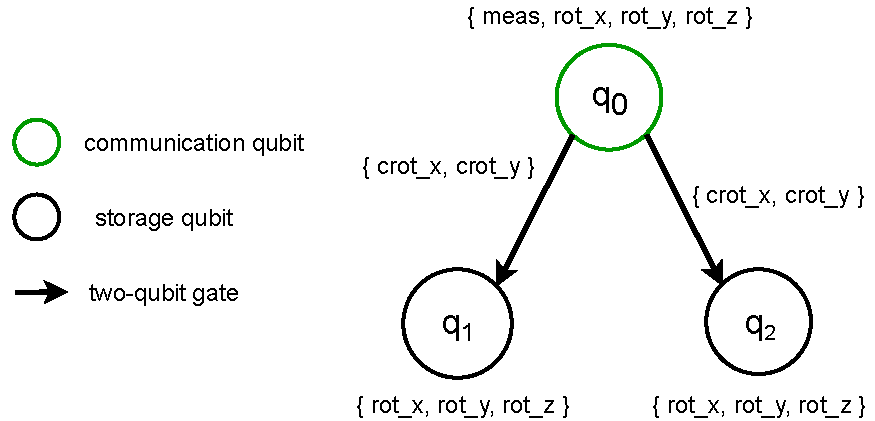
\includegraphics[width=0.7\textwidth]{figures/netqasm/unit-module.pdf}
      \caption{Example of a unit-module topology on a platform using
            nitrogen-vacancy centers in diamond. A unit-module is a
            hypergraph~\cite{berge1984hypergraphs}, with associated information
            on both nodes and edges. Each node represents a virtual qubit,
            containing information about (1) its qubit type (communication or
            storage), (2) physical properties of the qubit, such as decoherence
            times and (3) which single-qubit gates are supported on the qubit,
            together with their duration and noise. Each edge represents the
            possibility of performing joint operations on those qubits, such as
            two-qubit gates, and also containing information about gate
            durations and noise.}\label{fig:topology}
\end{figure}



\subsection{NetQASM language}

\subsubsection{Instructions}
\label{sec:design_decisions_language}
As explained in~\cref{sec:design_decisions_interface}, the \host delegates quantum code (including limited classical control) of the program to the \QNPU by creating blocks of instructions and sending these to the \QNPU for execution.
These blocks are called subroutines and contain \netqasm \textit{instructions}.
Since the \QNPU is meant to be limited in processing power, the instruction set that it interprets should also be simple and low-level.
The \netqasm instruction set contains instructions for simple arithmetic, classical data manipulation, and simple control flow in the form of (un)conditional branch instructions.
Although conditional control-flow can be done at the \host as well, \netqasm branching instructions allow for much faster feedback since they are executed by the \QNPU, and hence cover the design consideration of real-time conditionals (\cref{sec:design_considerations}).
We note the obvious performance gain by being able to do control logic without having to go back to the \host.
There are no higher-level concepts such as functions or for-loops, which would require more complicated and resource-demanding parsing for the \QNPU, such as constructing an abstract syntax tree.

A single instruction specifies an operation, possibly acting on classical or quantum data.
For example, a single-qubit rotation gate is represented as an instruction containing the type of gate, the classical register containing the rotation angle, and the classical register containing the virtual ID of the qubit (as specified in the unit module) to act on.
\netqasm specifies a set of \textit{core} instructions that are expected to be implemented by any \QNPU.
These include classical instructions like storing and loading classical data, branching, and simple arithmetic.
Different hardware platforms support different quantum operations.
\netqasm should also support platform-specific optimization (\cref{sec:design_considerations}).
Therefore, \netqasm uses \textit{flavors} of quantum instructions (\cref{sec:design_decisions_flavours}).
The \textit{vanilla} flavor consists universal of a set of platform-independent quantum gates.
Particular hardware platforms, such as the NV-centre, may use a special NV flavor, containing NV-specific instructions.
A \QNPU implementation may use a custom mapping from vanilla instructions to platform-specific ones.
The instructions in a flavor are also called a software-visible gate set~\cite{murali2019fullstack}.
See~\cref{app:instructions} for more details on \netqasm instructions.

\subsubsection{Remote entanglement generation}
Generating entanglement with a remote node is also specified by instructions.
These are however somewhat special compared to other instructions.
First, entanglement generation has a non-deterministic duration.
Therefore, when an entanglement instruction is executed, the request is forwarded to the part of the system responsible for creating entanglement, but the instruction itself immediately returns.
A separate \textit{wait} instruction can be used to block on entanglement generation to actually be completed.
Second, entanglement generation requests should be compatible with the network stack proposed in~\cite{dahlberg2019linklayer}, including the network layer from~\cite{kozlowski2020networklayer}.
These requests need to be accompanied by information such as the number of EPR pairs to generate or the minimum required fidelity.
Third, this information should be able to depend on runtime information.
For example, the required fidelity may depend on an earlier measurement outcome.
Therefore, entanglement generation parameters cannot be static data, and must be stored in arrays.
Furthermore, the result of entanglement generation with the remote node consists of a lot of information, such as which Bell state was produced, the time it took, and the measurement results in case of measuring directly.
This information is written by the \QNPU to an array which is specified by the entanglement instruction.
Finally, since writing the information to the array indicates that entanglement generation succeeded, the wait instruction can be used to wait until a certain array is filled in, such as the one provided by the entanglement instruction.
Since the entanglement instruction is non-blocking, it is possible to continue doing local operations while waiting for entanglement generation to complete.

We assume that the \QNPU implements a network stack where connections need to be set-up between remote nodes before entanglement generation can happen~\cite{kozlowski2020networklayer, dahlberg2019linklayer}.
\netqasm provides a way for programs to open such connections in the form of \textit{EPR sockets}.
The \host can ask the \QNPU to open an EPR socket with a particular remote node.
The \QNPU is expected to set up the required connections in the network stack, and associates this program socket with the connection.
When the program issues an instruction for generating entanglement, it refers to the EPR socket it wants to use.
Based on this, the \QNPU can use the corresponding connection in the network.


\begin{figure}
      \centering
      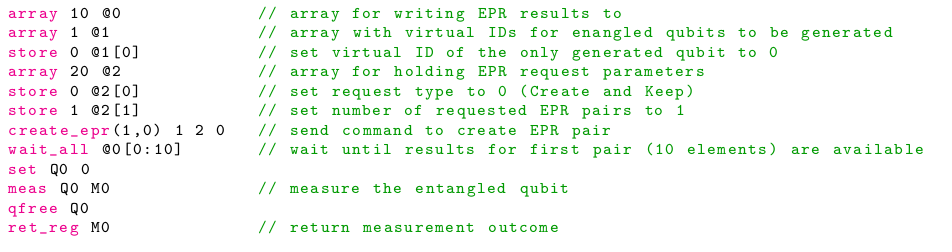
\includegraphics[width=0.7\textwidth]{figures/netqasm/nqasm_code_example}
      \caption{Example of NetQASM code for generating a single entangled pair with another node followed by a measurement.
            See the Appendix for more details of the instructions.}
      \label{fig:nqasm_code_example}
\end{figure}

\subsubsection{Flavors}
\label{sec:design_decisions_flavours}
We want to keep \netqasm platform-independent.
However, we also want the potential for platform-specific optimization (\cref{sec:design_considerations}).
Therefore we introduce the concept of \textit{flavors}.
Flavors only affect the quantum instruction set of the language, and not the memory model or the interaction with the \QNPU.
We use the \textit{vanilla} or generic flavor for a general, universal gate set.
Subroutines may be written or generated in this vanilla flavor.
Platform-independent optimization may be done on this level.
A \QNPU may directly support executing vanilla-flavored \netqasm.
Platform-specific translations may then be done by the \QNPU itself.
It can also be that a \QNPU only supports a specific flavor of \netqasm.
A reason for this could be that the \QNPU does not want to spend time translating of the instructions at runtime.
In this case, the \host should perform a translation step from the vanilla flavor to the platform-specific flavor.
In such a case, the vanilla flavor can be seen as an \textit{intermediate representation}, and the translation to a specific flavor as a back-end compilation step.

\subsubsection{Programmability}
Since the \netqasm instructions are relatively low-level, we like to have a higher-level programming language for writing programs, that is automatically compiled to \netqasm.
We introduce a higher-level SDK in \cref{sec:python-sdk}.
However, we do not see this as part of the \netqasm specification itself.
This decoupling allows the development of SDKs to be independent such that these can be provided in various languages and frameworks.

We still want \netqasm instructions to be suitable for manual writing and inspection.
Therefore, instructions (and subroutines) have two formats: a binary one that is used when sending to the \QNPU, and a text format that is human-readable.
The text format resembles assembly languages including \openqasm.
Examples are given in \cref{sec:sdk} and the Appendix.


\section{Python SDK}
\label{sec:python-sdk}
We implemented \netqasm\ by developing a Software Development Kit (SDK) in Python.
This SDK allows a programmer to write quantum network programs as Python code, including the quantum parts.
These parts are automatically translated to NetQASM subroutines.
The SDK contains a simulator that simulates a quantum network containing end-nodes, each with a \QNPU.
The SDK can execute programs by executing their classical parts directly and executing the quantum parts as \netqasm subroutines on the simulated \QNPU.
By executing multiple programs at the same time, on the same simulated network, a whole multi-partite application can be simulated.
In~\cref{sec:evaluation} we use this SDK to evaluate some of the design decisions of \netqasm.

We refer to the docs at~\cite{git_netqasm} for the latest version of the SDK.
Below, we give an example of an application written in the SDK to give an idea of how development in the SDK looks like.
In \cref{app:examples_sdk} we provide a few more examples of applications in the SDK and their corresponding \netqasm\ subroutines.

All code can be found at~\cite{git_netqasm} and~\cite{git_squidasm}, including:
    (1) Tools for serializing (de-serializing) to (from) both human-readable text form and binary encoding,
        % \item A parser for the human-readable form of \netqasm.
        % \item A parser for binary encoding of \netqasm.
        % \item An assembler of human-readable form to binary.
    (2) the \netqasm\ SDK, together with compilers (no optimization yet),
    (3) support for running applications written in the SDK on the simulators \netsquid~\cite{netsquid,coopmans2021netsquid} and \simulaqron~\cite{dahlberg2018simulaqron}, and
    (4) implemented applications in \netqasm, including: anonymous transmission~\cite{Christandl2005anonymous}, BB84~\cite{bb84}, blind quantum computing~\cite{broadbent2009universal,fitzsimons2017unconditionally}, CHSH game~\cite{Kaniewski2016}, performing a distributed CNOT~\cite{denchev2008distributed}, magic square game~\cite{brassard1999magicsquare}, teleportation~\cite{bennett1993teleporting}.

\subsection{SDK}
\label{sec:sdk}
The SDK of \netqasm\ uses a similar framework to the SDK used by the predecessor \cqc~\cite{git_cqc}.
Any program on a node starts by setting up a \texttt{NetQASMConnection} to the \QNPU-implementation in the \emph{backend}.
The \texttt{NetQASMConnection} encapsulates all communication that the \host\ does with the \QNPU.
More information about supported backends can be found below in \cref{sec:backends}.
Using the \texttt{NetQASMConnection} one can for example construct a \texttt{Qubit} object.
The \texttt{Qubit} object has methods for performing quantum gates and measurements.
When these methods are called, corresponding \netqasm\ instructions are included in the current subroutine being constructed.
One marks the end of a subroutine, and the start of another, either by explicitly calling \texttt{flush} on the \texttt{NetQASMConnection} or by ending the scope of the \nq{with NetQASMConnection ...} context.

The following Python code shows a basic application written in the \netqasm\ SDK.
The application will be compiled into a single subroutine executed on the \QNPU, which creates a qubit, performs a Hadamard operation, measures the qubit and returns the result to the application layer.
% \subsubsection{Hello world/Hello Hadamard}
% Functionally the same as the \netqasm-subroutine~\ref{sec:example_nq_hello_world}.
\begin{pycode}
  # Setup connection to backend
  # as the node Alice
  with NetQASMConnection("Alice") as alice:
    # Create a qubit
    q = Qubit(alice)
    # Perform a Hadamard on the qubit
    q.H()
    # Measure the qubit
    m = q.measure()
    # The end of the context also marks
    # the end of the subroutine
    # automatically but can also be done
    # explicitly using `alice.flush()`
\end{pycode}

The following \netqasm\ subroutine is the result of translating the above Python code to \netqasm of the vanilla (platform-independent) flavor.

% \subsubsection{Hello world/Hello Hadamard}\label{sec:example_nq_hello_world}
% A simple subroutine which creates a qubit, performs a Hadamard, measures the qubit and returns the measurement outcome to the host.
\begin{nqcode}
  # NETQASM 1.0
  # APPID 0
  // Set the virtual qubit ID to use
  set Q0 0

  // Allocate and initialize a qubit
  qalloc Q0
  init Q0

  // Perform a Hadamard gate
  h Q0

  // Measure the qubit
  meas Q0 M0

  // Return the outcome
  ret_reg M0
\end{nqcode}

\subsubsection{Backends}
\label{sec:backends}
As mentioned above, the \texttt{NetQASMConnection} in the SDK is responsible for communicating with the implemented \QNPU\ in the \emph{backend}.
The \emph{backend} can either be a simulator or an actual \QNPU\ using real quantum hardware.
Currently supported backends are the simulators \squidasm~\cite{git_squidasm} (using \netsquid~\cite{netsquid, coopmans2021netsquid}) and \simulaqron~\cite{dahlberg2018simulaqron}.
A physical implementation of \QNPU\ running on quantum hardware is being worked on at the time of writing.
Using the SDK provided at~\cite{git_netqasm}, one can for example simulate a set of program files for the nodes of a quantum network on \netsquid\ using a density matrix formalism with the command:
\begin{nqcode}
  netqasm simulate --simulator=netsquid --formalism=dm
\end{nqcode}
For more details see the docs at~\cite{git_netqasm}.


\section{Evaluation}
\label{sec:evaluation}
We evaluate two of the design choices that we made for \netqasm:
    (1) exposing unit-modules to the \host and
    (2) adding the possibility to use platform-specific flavors of instructions.
For both elements we study the difference in including them in \netqasm versus not including them.
We do this by simulating a teleportation application and a blind quantum computation application.
These examples also showcase the ability of \netqasm to express general quantum internet applications.

We have implemented a simulator, called \squidasm~\cite{git_squidasm}, that simulates a network in which end-nodes have the internal architecture as described in~\cref{sec:preliminaries}, that is, with an \host and a \QNPU.
The simulator internally uses NetSquid~\cite{netsquid}, which was made specifically for the simulation of quantum networks.
\squidasm executes programs written using the SDK (\cref{sec:python-sdk}), including sending \netqasm subroutines to the (simulated) \QNPU.
The code and data that were used to produce the results in this section can be found at~\cite{git_netqasm_paper_data}.

We evaluate the performance of \netqasm by looking at the runtime quality of two applications, both consisting of two programs (one per node).
The first is a teleportation of a single qubit from a sender node to a receiver node.
We define the quality as the fidelity between the original qubit state at the sender and the final qubit state at the receiver.
The second application is a blind computation protocol which involves a client and a server.
The server effectively performs, blindly, a single-qubit computation on behalf of the client.
The protocol is a so-called \textit{verifiable blind quantum computation}~\cite{fitzsimons2017unconditionally}.
This means that some of the rounds of the protocols are \textit{trap rounds}.
We define the quality that we evaluate as the error rate of these trap rounds, since this indicates the blindness of the server.

We run these applications on \squidasm, where we simulate realistic quantum hardware.
Specifically, we simulate nodes based on nitrogen-vacancies (NV) in diamond, that can do heralded entanglement generation between each other.
The simulated hardware uses noise models that are also used in~\cite{coopmans2021netsquid}.
For more details, see~\cref{app:simulation}.

A note on how we chose what to evaluate and what not.
We listed several design considerations in ~\cref{sec:design_considerations}.
We addressed these in our design decisions (\cref{sec:design_decisions}).
For some of these, it is straightforward to see how they address a certain consideration, such as conditionals allowing for fast runtime feedback, and unit modules for allowing multitasking, as explained in~\cref{sec:design_decisions}.
Also, fundamental requirements like remote-entanglement generation and shared memory have been addressed.
The remaining considerations, and our solutions, namely platform independence and memory virtualization using unit modules, are less trivial to evaluate just by looking at the design.
Therefore, we focus on the evaluation of these two design decisions.

In our evaluation, we focus specifically on the Nitrogen-Vacancy hardware for our nodes.
This has two reasons.
First, it is a promising hardware platform for quantum network nodes~\cite{Taminiau2014} which we know quite well since it is available in the lab, and we have even used \netqasm in a simple test case running on nodes based on NV~\cite{pompili2021experimental}.
Second, the NV hardware is interesting since it has a restricted gate set and qubit topology, which is explained in more detail below.
Therefore, we expect that the use of unit modules and an NV-specific flavor makes a difference in terms of runtime quality.

\subsection{Unit modules}
\label{sec:evaluation-unit-modules}
We ask ourselves the question whether it pays off to expose unit modules, that is, a qubit topology with gate- and entanglement information.
Specifically, we want to know if there are situations where knowing the unit module gives the \host an opportunity to optimize the application in a way that is not possible when not knowing the unit module.
If so, we are interested in how much advantage this gives (in terms of the runtime quality defined above).

In the next section we show that there are indeed situations where knowledge of the unit module is advantageous.
It can be that the order in which \netqasm instructions are issued in a subroutine is sub-optimal, since virtual qubit IDs may be mapped in such a way that the \QNPU has to move virtual qubits to different physical qubits in order to execute the instructions.
If the \host layer does not know this mapping, it cannot know that the instructions are ordered sub-optimally.
With knowledge of the unit module, on the other hand, the \host can optimize the order and the overall application performance is improved.

We consider a teleportation application where a \textit{sender} program teleports a single qubit to another \textit{receiver} program.
It is assumed that the underlying platform is based on nitrogen-vacancy centers in diamond (NV) and use well-established models for both the noise and operations supported on such platforms, see \cref{app:simulation}.
The sender program uses two qubits: one to create entanglement with the receiver (qubit E), and one to send (teleport) to the receiver (qubit T).
At some point, the sender measures both qubits, after which it sends the outcomes to the receiver so that it can do the relevant corrections on its received qubit.
We assume that the sender program is written in a higher-level language like, like in our SDK (\cref{sec:sdk}), and in such a way that it first issues a measurement operation on qubit T, and then on E. However, due to the differences in characteristics of the physical qubits, as will be explained below, it is more efficient to first do the measurement on E, and then on T. Now we consider two scenarios, namely
\begin{itemize}
  \item \textbf{Unit-modules (UM)}.
        We assume that the sender program is written and executed on a software stack implementing \netqasm, which means that the application's view of its quantum working memory is in the form of a unit module.
        This unit module contains information about the above-mentioned hardware restrictions, and therefore a compiler can take advantage of it by re-ordering the measurement operations while generating the \netqasm subroutines to be sent to the \QNPU.
  \item \textbf{No unit-modules (NUM)}.
        In this case the software stack also implements \netqasm, but without unit modules.
        Specifically, the application sees its quantum memory as just a number of uniform qubits.
        Therefore, a compiler for this application does not know about the hardware restrictions, and will construct \netqasm-subroutines sent to the \QNPU\ without doing any optimization and leaves the order of the operations to be performed as they are specified in the high-level SDK.
\end{itemize}

Let's first go through the steps of the teleportation application:\newline
\begin{description}
  \item[\textit{sender}]:
        \begin{enumerate}
          \item Initialize qubit $q_t$ to be teleported in a Pauli state.
          \item Create entanglement with \textit{receiver} using qubit $q_s$.
          \item Perform CNOT gate with $q_t$ as control and $q_s$ as target.
          \item Perform Hadamard gate on $q_t$.
          \item Measure qubit $q_t$ and store outcome as $m_1$.
          \item Measure qubit $q_s$ and store outcome as $m_2$.
          \item Send $m_1$ and $m_2$ to \textit{receiver}.
        \end{enumerate}
  \item[\textit{receiver}]:
        \begin{enumerate}
          \item Receive entanglement with \textit{sender} using qubit $q_r$.
          \item Receive measurement outcomes from \textit{sender}.
          \item Apply correction operations on $q_r$ based on measurement outcomes.
        \end{enumerate}
\end{description}

We will now consider the order of the steps of the \textit{sender}.
Firstly, we assume that the qubit to be teleported, $q_t$, is always created before the entanglement.
We motivate this assumption below. For this reason, steps 1--3 and 7 are fixed and cannot change.
However, we are free to do step 6 before step 4 and 5, since these single-qubit operations and measurements commute, as long as we are consistent with the outcomes $m_1$ and $m_2$.
Let's now consider what impact this decision of measuring $q_s$ before $q_t$ or not has on the quality of execution for a NV-platform.

One of the biggest restrictions on a NV-platform is the topology of the qubits.
In particular, the NV-platform has a single communication-qubit (electron) surrounded by some number of storage qubits (carbon spins), see for example \cref{fig:topology}.
The single communication qubit is not only responsible for any remote entanglement generation but also for any two-qubit gate and is the only qubit that can be directly measured.
These restrictions require qubit states to be moved back and forth between the communication qubit and the storage qubits in order to free up the communication qubit, to create new entanglement or to measure another qubit.
Since the operation of moving a qubit state is relatively slow on this platform (up to a millisecond~\cite{Humphreys2018}) and adds noise to the qubits, it is important to try to minimize the number of moves needed.
For more details on the NV-platform, see for example~\cite{Bernien2014} or~\cite{dahlberg2019linklayer}.

In the steps of the \textit{sender} above, the communication qubit is first initialized to a Pauli state.
This state is then moved to a storage qubit to free up the communication qubit in order to create entanglement with the \textit{receiver}.
Then in step 5, $q_t$ should be measured, which is currently in the storage qubit.
This requires the qubit state to first be moved to the communication qubit.
However, at this point the communication qubit is occupied by the entangled pair and therefore first needs to be moved to a second storage qubit.
Qubit $q_t$ can then be moved to the communication qubit to be measured and then the same is done for $q_s$, requiring in total four move operations and three physical qubits.

We can now see that performing step 6 before 4 and 5 has the advantage that this qubit is already in the communication qubit and can be measured directly without moving it first.
Afterwards, $q_t$ can be moved to the communication qubit, which is cleared after the measurement, requiring in total only 2 move operations and only two physical qubits.
The decision of performing step 6 before 4 and 5 is highly dependent on the NV-platform and can only be made by a compiler that is aware about these restrictions.
The inclusion of unit-modules and qubit types in the \netqasm-framework, which are exposed to the compiler at the \host, allows for these optimization decision and can therefore improve the quality of execution.

For the two scenarios we consider, i.e. performing step 6 before 4 and 5 (\textbf{Unit modules (UM)}) or not (\textbf{No unit-modules (NUM)}), we check the average fidelity of the teleported state as a function of the gate noise (\cref{fig:sweep_gate_noise}), as well as the average fidelity and execution time as a function of gate duration (\cref{fig:sweep_gate_noise}), of the native two-qubit gate of the NV-platform. We see that performing step 6 before 4 and 5 improves both total execution time and average fidelity.
This can be explained by the fact that using unit modules allowed a compiler to produce \netqasm code containing fewer two-qubit gates.
Therefore, an increase in two-qubit gate noise leads to a lower fidelity.
Also, an increase in two-qubit gate duration leads to higher execution time difference between the two scenarios.
Finally, \cref{fig:sweep_gate_noise} shows that the two-qubit gate duration does not affect the final fidelity in this situation, but the difference between using unit modules versus not using them remains.


\begin{figure}
    \centering
    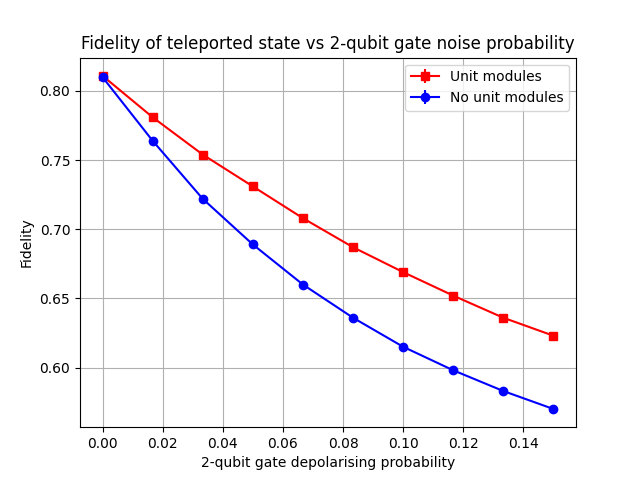
\includegraphics[scale=0.8]{figures/netqasm/plots/paper_teleport_sweep_gate_noise.png}
    \caption{
        Average fidelity between the original state at the sender and
        the final state at the server, as a function of the depolarizing noise
        of the native two-qubit gate of the NV-platform, both for the case of
        performing step 6 after (\textbf{No unit modules}) and before
        (\textbf{Unit modules}) step 4 and 5. Execution time of the native
        two-qubit gate is set to 0.5 ms. The rest of the parameters used are
        listed in \cref{app:simulation}. Each point is the average over each of
        the six Pauli states as initial state, repeated 100 times.}
    \label{fig:sweep_gate_noise}
\end{figure}

\begin{figure}
    \centering
    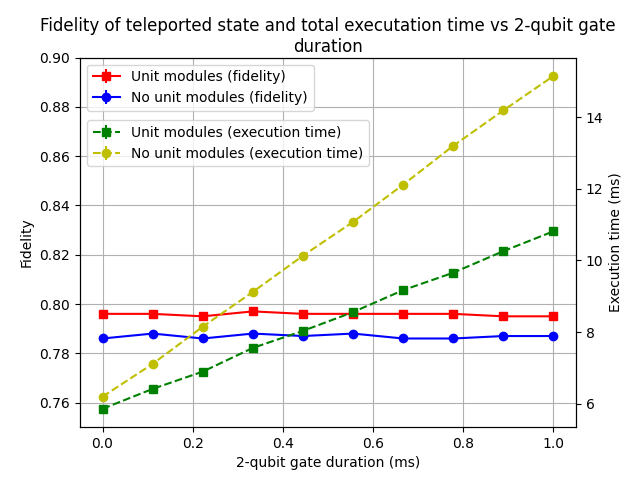
\includegraphics[scale=0.8]{figures/netqasm/plots/paper_teleport_sweep_gate_time.png}
    \caption{
        Average fidelity of the teleported state (left y-axis, solid lines) and total
        execution time of the teleportation application (right y-axis, dashed
        lines) as a function of the execution time of the native two-qubit gate
        of the NV-platform, both for the case of performing step 6 after
        (\textbf{No unit modules}) and before (\textbf{Unit modules}) step 4 and
        5. Dephasing parameter of the native two-qubit gate is set to 0.02. The
        rest of the parameters used are listed in \cref{app:simulation}. Each
        point is the average over each of the six Pauli state as initial state,
        repeated 100 times. In both figures, error bars are smaller than the drawn
        dots.}
  \label{fig:sweep_gate_time}
\end{figure}



\subsection{Flavors}\label{sec:evaluation-flavours}
While aiming to let \netqasm be mostly platform-independent, we did also choose to allow platform-specific instructions, bundled in flavors.
The idea is that this allows for platform-specific optimization leading to better application performance.
Here we evaluate if flavors really impact potential performance, and if so how much.

We show that platform-specific optimization can indeed improve application performance, and that there are such optimizations that are not possible without flavors.
We see that it has impact mostly on the execution time, but not necessarily on outcome quality.

We consider the blind computation application depicted in \cref{fig:bqc_app}, where both the client and server node implement the NV hardware.
Again we compare two scenarios, in this case:
\begin{itemize}
  \item \textbf{Vanilla}.
        We compile both the client's and server's application code to \netqasm subroutines with the vanilla flavor.
        The \QNPU, controlling NV hardware which does not implement all vanilla gates natively, needs to translate the vanilla instructions on the go.
        We assume this translation is ad-hoc and does not do any optimizations like removing redundant gates.
  \item \textbf{NV}.
        The code is compiled to \netqasm subroutines containing instructions in the NV flavor, and redundant gates are optimized away.
        The \QNPU can directly execute the instructions on the hardware.
\end{itemize}

We implemented this by writing two separate programs in the SDK, one for the client and one for the server.
The SDK automatically compiles the relevant parts of these programs into \netqasm subroutines.
Classical communication (values $\delta_1$, $m_1$ and $\delta_2)$ is done purely between the two simulated application layers, so these operations are not compiled to \netqasm subroutines.
More details about the simulation can be found in \cref{app:simulation}.

The protocol is a verifiable blind quantum protocol~\cite{fitzsimons2017unconditionally}, which means that the circuit in~\cref{fig:bqc_app} is run multiple times, namely once per round.
Some of these rounds are \textit{trap rounds} in which the client chooses a special set of input values.
Such a trap round can either succeed or fail, depending on the values returned by the server.
The fraction of trap rounds that fail is called the error rate.
The error rate should stay low in order for the computation to be blind.

We simulate the BQC application by running the client's and server's programs in \squidasm.
We look at the error rate of the trap round as a function of the two-qubit gate noise.
The result can be seen in~\cref{fig:plot_bqc}.
It can be seen that using the NV flavor provides a better (lower) error rate than using the vanilla flavor.
This can be explained by noting that \netqasm instructions in the vanilla flavor are mapped ad-hoc to native NV gates by the \QNPU at runtime, which leads to more two-qubit gates in total.


\begin{figure}
  \centering
  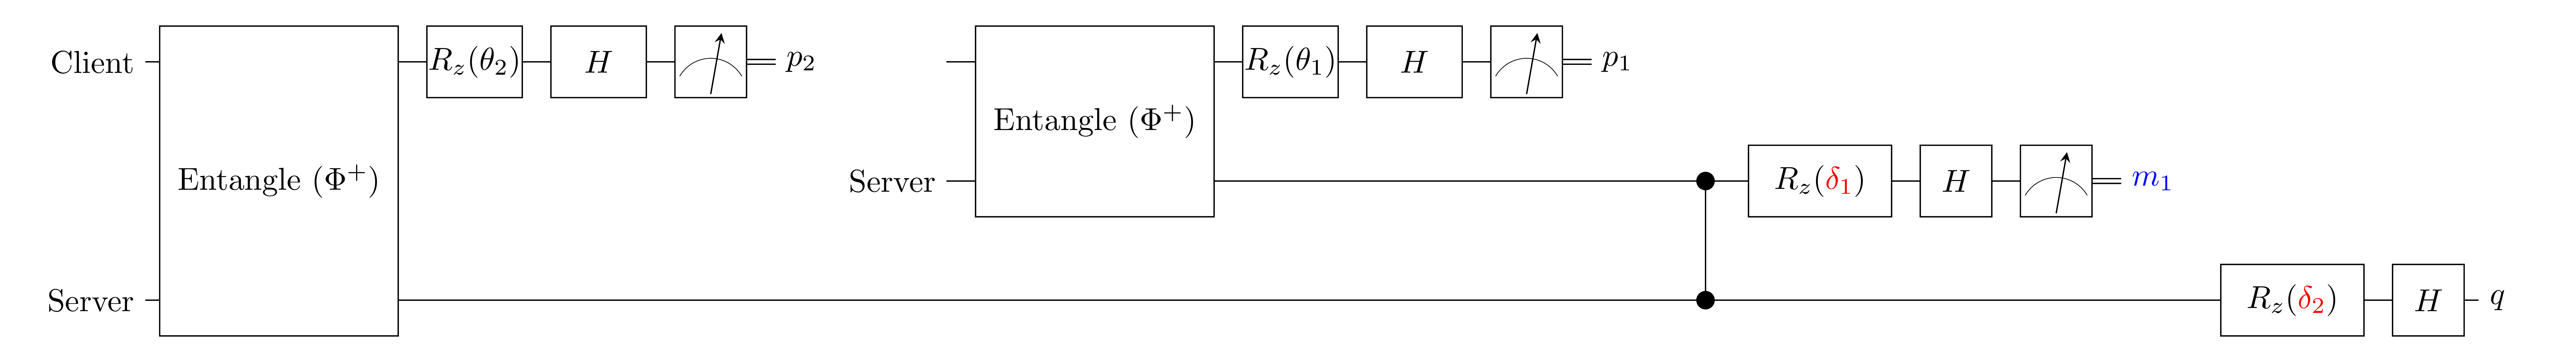
\includegraphics[width=\textwidth]{figures/netqasm/bqc_app.png}
  \caption{Circuit representation of the simulated BQC application. The client
    remotely prepares two qubits on the server, by twice creating an
    entangled pair with the server followed by a local measurement. The
    server locally entangles its two qubits (cphase gate). Then, the client
    and server use classical communication to further guide the server's
    quantum operations. The client computes $\delta_1 = \alpha - \theta_1 +
      p_1 \cdot \pi$ and sends this to the server. The server uses the
    received value to do a local rotation and later sends measurement
    outcome $m_1$ back to the client. The client then sends $\delta_2 =
      (-1)^{m_1} \cdot (\beta - \theta_2 + p_2 \cdot \pi)$ to the server.
    The qubit state $q$ is the result of this application.
  }
  \label{fig:bqc_app}
\end{figure}


\begin{figure}
  \centering
  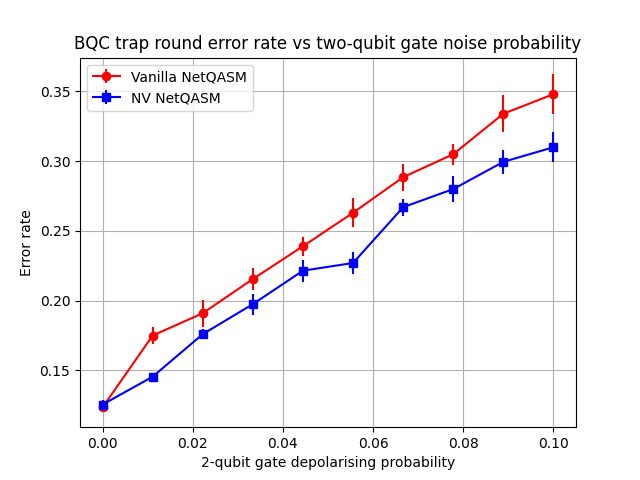
\includegraphics[scale=0.8]{figures/netqasm/plots/bqc_sweep_gate_noise_trap.png}
  \caption{
    Average error rate of trap rounds for the circuit of~\cref{fig:bqc_app}.
    Each point is the average over four combinations of $\theta_1$ and $\theta_2$,
    each used in 500 trap rounds. It can be seen that using the vanilla (platform-independent)
    \netqasm flavor results in a worse (higher) error rate on average.}
  \label{fig:plot_bqc}
\end{figure}

To gain some more insight into why using the NV flavor provides a lower error rate we also look at the fidelity of the two quantum states on the server before any local gates are applied.
As can be seen in~\cref{fig:bqc_app}, the client remotely prepares two states on the server by twice creating entanglement and measuring its own half of the EPR pair.
In~\cref{fig:plot_bqc_fidelity} we see that already during this remote state preparation phase the NV flavor outperforms the vanilla flavor in terms of the fidelity of the prepared states.

\begin{figure}
  \centering
  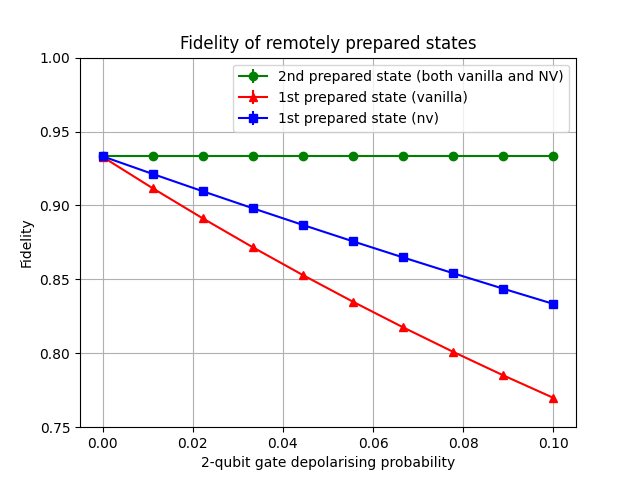
\includegraphics[scale=0.8]{figures/netqasm/plots/bqc_sweep_gate_noise_epr_fidelity.png}
  \caption{ Fidelity of the two remotely prepared states on the server in
        the BQC application. To remotely prepare a state, the client and server
        first create an EPR pair, and the client then measures its half in a
        specific basis while the server keeps its half stored in the
        communication qubit. This first prepared state is then moved to a memory
        qubit to free up the communication qubit for preparing the second state.
        This move operation has a negative effect on the fidelity of the first
        prepared state. Since the fidelity of the second prepared state only
        depends on the link entanglement generation, there is no difference
        between using vanilla or NV instructions. The values are from the same
        simulation experiment as for ~\cref{fig:plot_bqc}. Error bars are
        negligible.}
  \label{fig:plot_bqc_fidelity}
\end{figure}

\subsection{Relation to other results}
We note that a similar question of how many physical details to expose from lower-level layers (in our case the \QNPU) to higher-level layers (in our case the \host) has also been evaluated in~\cite{murali2019fullstack}.
Their conclusion is that exposing and leveraging some of these details can indeed improve certain program success metrics.
That result agrees with that of ours, which shows that program execution quality can improve by exposing and leveraging unit modules and platform-specific \netqasm flavors.

\section{Conclusion}
\label{sec:conclusion}
\netqasm enables the development of quantum internet applications in a platform-independent manner.
It solves the question of dealing with the complexity of having both classical and quantum operations in a single program, while at the same time providing a relatively simple format for \QNPU-like layers to handle.
Multiple applications, such as remote teleportation and blind quantum computation, have already been implemented.
A simple compiler has been implemented that can translate code written in the higher-level SDK into \netqasm.

Additionally to the work in this paper, we are also developing a physical implementation of the \QNPU.
One key component in this implementation is the \emph{Quantum Node Operating System} (\qnodeos), which acts as the bridge between the applications and the physical layer.
\qnodeos\ will be presented in a dedicated paper including results of a first integration test between \netqasm, \qnodeos\ and underlying physical quantum hardware.
This will mark the first time a quantum network node has been programmed using platform-independent code.


\section{Acknowledgments}
We thank Arjen Rouvoet and \"Onder Karpat for valuable discussions.
This work was supported by ERC Starting Grant, EU Flagship on Quantum Technologies, Quantum Internet Alliance, NWO VIDI.


\section{Data availability}
The data that support the findings of this study are openly available at the following URL/DOI: \url{https://github.com/QuTech-Delft/netqasm-paper-data}.

\section{Flow of messages}
\label{sec:app-messages}
Here we define the content of each of the messages being sent between the \host and the \QNPU.
Each message has an ID chosen by the \host\ which is used to associate replies from the \QNPU\ to the \host.
\begin{itemize}
  \item \nq{RegisterApp}:
        Sent once from the \host\ to the \QNPU\ whenever a new application starts.
        Contains information on what resources are required by the application, in particular:
        \begin{itemize}
            \item \nq{unit_module_spec}: Specification of unit-module needed, e.g. number of qubits.
            \item \nq{epr_socket_spec}: Specification of EPR sockets needed, see~\cite{kozlowski2020networklayer}, containing
                (1) EPR socket ID,
                (2) remote node ID,
                (3) remote EPR socket ID and
                (4) minimum required fidelity.
        \end{itemize}
  \item \nq{RegisterAppOK}:
            Returned from the \QNPU\ when application is registered, containing an application ID to be used for future messages.
            \begin{itemize}
                \item \nq{app_id}: Application ID.
            \end{itemize}
  \item \nq{RegisterAppErr}:
        Returned from the \QNPU\ when registration of application failed.
        For example if required resources could not be met.
        \begin{itemize}
            \item \nq{error_code}: Error code specifying what went wrong.
        \end{itemize}
  \item \nq{Subroutine}:
        Message from the \host\ to the \QNPU, containing a subroutine to be executed.
        Details on the content are presented in later sections.
        \begin{itemize}
            \item \nq{app_id}: Application ID.
            \item \nq{subroutine}: The subroutine to be executed.
        \end{itemize}
  \item \nq{Done}:
        Message from the \QNPU\ to the \host, indicating that a subroutine has finished.
        Which subroutine is indicated by the message ID.
        \begin{itemize}
            \item \nq{message_id} Message ID used for the \nq{Subroutine}-message.
        \end{itemize}
  \item \textbf{Update memory}:
        The \host\ will have access to a copy of the memory allocated by the \QNPU\ for certain registers and arrays, see \cref{sec:language}.
        This memory is read-only by the \host.
        Updates to the copy of the memory are performed by the end of a subroutine or if the subroutine is waiting.
        Furthermore, updates need to be explicitly specified in the subroutine by using one of the return-commands.
        How the actual update is implemented depends on the platform and can either be done by message-passing or with an actual shared memory.
        However, the subroutine is independent from this implementation.
        The \host\ will be notified by an explicit message whenever the memory is updated.
  \item \nq{StopApp}:
        Sent from the \host\ to the \QNPU\ indicating that an application is finished.
\end{itemize}


\section{Operands}\label{sec:operands}
In this section we give the exact definition of the types of operands used in the \netqasm\ language.
Each instruction of \netqasm\ takes one or more operands.
There are five types of operands, which are listed and described below.
Each instruction has a fixed types of operands at each position.
The exact operands for each instruction is listed in \cref{app:instructions}.
We note also that in the human-readable text-form of \netqasm, there are also \textit{branch variables}.
However, these are always replaced by \IMMEDIATE{}s (constants), corresponding to the instruction number of the subroutine, before serializing, see \cref{sec:branch_variables}.

The operand types of \netqasm\ are:
\begin{itemize}
  \item \IMMEDIATE (constant): An integer seen as it's value.
        The following instruction, \nq{beq} \emph{branch-if-equal}, branches to instruction index \nq{12} since the number \nq{0} equals the number \nq{0}.
        \begin{nqcode}
beq 0 0 12\end{nqcode}
        In the binary encoding used at~\cite{git_netqasm}, \IMMEDIATE{}s are \nq{int32}.
  \item \REGISTER: A register specifying a register name and a index.
        The following instruction sets index \nq{0} of the register name \nq{R} to be \nq{0}.
        \begin{nqcode}
set R0 0\end{nqcode}
        In the current version of \netqasm\ there are four register names and the indices are relative to the names.
        They are all functionally the same but are meant to be used for different purposes and increase readability:
        \begin{itemize}
          \item \nq{C}: Constants, meant to only be \nq{set} once throughout a subroutine.
          \item \nq{R}: Normal register, used for looping etc.
          \item \nq{Q}: Stores virtual qubit IDs.
          \item \nq{M}: Stores measurement outcomes.
        \end{itemize}
        In the binary encoding used at~\cite{git_netqasm}, \REGISTER{}s are specified by one byte and hold one \nq{int32}.
  \item \ADDRESS: Specifies an address to an array.
        Starts with \nq{@}.
        The following instruction declares an array of length \nq{10} at address \nq{0}.
        \begin{nqcode}
array 10 @0\end{nqcode}
        For more information about arrays, see below.
        The address here is just an identifier of the array and does not refer to a actual memory address.
        For this reason \nq{@1} above does not mean the second entry of the declared array but simply a different array.
        Addresses are relative to the application ID and are valid across subroutines.
  \item \textbf{ARRAY\_ENTRY}: Specifies an entry in an array.
        Takes the form \nq{@a[i]}, where \nq{a} specifies the address and \nq{i} the index.
        The following instruction stores the value of \nq{R0} to the second entry of the array with address \nq{0}.
        \begin{nqcode}
store R0 @0[1]\end{nqcode}
        In the text-form \nq{i} can either be an \IMMEDIATE\ or a \REGISTER, however in the binary encoding used at~\cite{git_netqasm}, \nq{i} is always a \REGISTER.
        This is handled by the compiler by using a \nq{set}-command before.
  \item \textbf{ARRAY\_SLICE}: Specifies a slice of an array.
        Takes the form \nq{@a[s:e]}, where \nq{a} specifies the address, \nq{s} the start-index (inclusive) and \nq{e} the end-index (exclusive).
        The following instruction waits for the second to the fourth entry of array with address \nq{0} to become not \nq{null}, see \cref{app:waiting}.
        \begin{nqcode}
wait_all @0[1:4]\end{nqcode}
        In the text-form \nq{s} and \nq{e} can either be an \IMMEDIATE{}s or a \REGISTER{}s, however in the binary encoding defined used at~\cite{git_netqasm}, \nq{s} and \nq{e} are always a \REGISTER{}s.
        This is handled by the compiler by using a \nq{set}-commands before.
\end{itemize}

\section{Branch variables}\label{sec:branch_variables}
The human-readable text-form of \netqasm\ supports the use of \emph{branch variables}.
Branch labels are declared as \nq{VAR}: before the instruction to branch to.
Before serializing a \netqasm-subroutine, all branch variables are replaced with \IMMEDIATE{}s corresponding to the correct \emph{instruction index}.
Delaying this replacement to the end is useful if the compiler wants to move around instructions.
For example if a subroutine is as follows:
\begin{nqcode}
# NETQASM 1.0
# APPID 0
set R0 0

// Loop entry
LOOP:
beq R0 10 LOOP_EXIT

// Loop body
// If statement
bge R0 5 ELSE
// true block
add R0 R0 1
jmp IF_EXIT
// false block
ELSE:
add R0 R0 2
IF_EXIT:

// Loop exit
jmp LOOP
LOOP_EXIT:\end{nqcode}
Which effectively does the same as the following program written in Python (where the variable \py{i} corresponds to the register \nq{R0} above).
\begin{pycode}
i = 0
while i != 10:
  if i < 5:
    i += 1
  else:
    i += 2
\end{pycode}
After replacing the branch labels the body of the subroutine will instead look:
\begin{nqcode}
store R0 0
beq R0 10 7
bge R0 5 5
add R0 R0 1
jmp 6
add R0 R0 2
jmp 1\end{nqcode}

\section{Arrays}
Classical data produced during the execution of a subroutine are stored in either fixed registers or allocated arrays.
Arrays in \netqasm\ have fixed-length, which is specified when declared using the \nq{array}-instruction.
Each entry of an array is an \emph{optional} \IMMEDIATE, meaning that the entry is an integer (e.g. \nq{int32}) or not defined (\nq{null}).
The arrays can be used to collect measurement outcomes to be returned to the \host\ but also other data such as information about the generated remote entanglement~\cite{dahlberg2019linklayer,kozlowski2020networklayer}.
All wait-instructions of \netqasm\ wait for one or more entries in an array to become defined (i.e. not \nq{null}).
The main use-case is for the execution of the subroutine to wait until the quantum network stack of the \QNPU\ has finished generated an entangled pair with a remote node.
The subroutine will be waiting for information about the entangled pair to be stored in a given array.
Once this is done, the execution can proceed.

The following subroutine for example creates and array with three elements, stores the values \nq{1} and \nq{2} to the array and reads them and adds them up, storing the value in the third entry.
\begin{nqcode}
// Create two constant registers
set C1 1
set C2 2
// Make an array of three entries
array 3 @0
// Load the constants to the array
store C1 @0[0]
store C2 @0[1]
// Load the array entries to two other registers
load R0 @0[0]
load R1 @0[1]
// Add the registers and store the result in the first
add R0 R1 R0
// Store the sum in the third entry of the array
store R0 @0[2]\end{nqcode}

\section{Qubit address operands}
Commands that perform actions on qubits have \REGISTER-operands which specify the virtual address of the qubit to act on.
It is good practice to use register name \nq{Q} for these registers.
The following subroutine performs a Hadamard gates on qubits with virtual addresses \nq{0}, \nq{1} and \nq{2}.
\begin{nqcode}
set Q0 0
set Q1 1
h Q0
h Q1
set Q0 2
h Q0\end{nqcode}
Note that \nq{Q0} is used twice but the value of the register is different.

\section{Instructions}\label{app:instructions}
\setlist[itemize]{leftmargin=*}
Here we list the current instructions part of the \textbf{vanilla flavor} of \netqasm.
For the most up to date version of the language, refer to~\cite{git_netqasm}.
Commands are specified as follows:
\begin{itemize}
  \item \nq{name}: Description of instruction.
        % Operands:
        \begin{enumerate}
          \item \IMMEDIATE : Description of op1
          \item \REGISTER : Description of op2
        \end{enumerate}
\end{itemize}

where \nq{name} is the name of the instruction, followed by the list of operands, specified by their type and description.
We note that in the human-readable text-form of \netqasm, it is allowed to provide an \IMMEDIATE\ for operands that are specified as \REGISTER.
The compiler will then replace these, using the \nq{set}-command.

\subsection{Allocation}

\begin{itemize}
  \item \nq{qalloc}: Start using a qubit in the unit module.
        % Operands:
        \begin{enumerate}
          \item \REGISTER: The virtual address of the qubit.
        \end{enumerate}
  \item \nq{array}: Creates an array of a certain length (width is fixed)
        % Operands:
        \begin{enumerate}
          \item \IMMEDIATE: Number of entries in the array.
          \item \ADDRESS: Address of array
        \end{enumerate}
\end{itemize}


\subsection{Initialization}

\begin{itemize}
  \item \nq{init}: Initializes a qubit to $|0\rangle$
        % Operands:
        \begin{enumerate}
          \item \REGISTER: The virtual address of the qubit.
        \end{enumerate}
  \item \nq{set}: Set a register to a certain value.
        % Operands:
        \begin{enumerate}
          \item \REGISTER: The register to assign a value to.
          \item \IMMEDIATE: The value to assign.
        \end{enumerate}
\end{itemize}

\subsection{Memory operations}
\begin{itemize}
  \item \nq{store}: Stores the value in a register to an index of an array.
        % Operands:
        \begin{enumerate}
          \item \REGISTER: The register holding the value to store.
          \item \textbf{ARRAY\_ENTRY}: The array-entry to store the value to.
        \end{enumerate}
  \item \nq{load}: Loads the value from an index of an array to a register.
        % Operands:
        \begin{enumerate}
          \item \REGISTER: The register to store the value to.
          \item \textbf{ARRAY\_ENTRY}: The array-entry holding the value.
        \end{enumerate}
  \item \nq{undef}: Sets an entry of an array to \nq{null}, see \cref{app:waiting}.
        % Operands:
        \begin{enumerate}
          \item \textbf{ARRAY\_ENTRY} Array-entry to make \nq{null}.
        \end{enumerate}
  \item \nq{lea}: Loads a given address of an array to a register.
        % Operands:
        \begin{enumerate}
          \item \REGISTER: The register to store the address to.
          \item \ADDRESS: The address to the array.
        \end{enumerate}
\end{itemize}

\subsection{Classical logic}

There are three groups of branch instructions: nullary, unary and binary.

\textbf{Nullary branching}
\begin{itemize}
  \item \nq{jmp}: Jump to a given line (unconditionally).
        % Operands:
        \begin{enumerate}
          % \item \IMMEDIATE: Line to branch to.
          \item \IMMEDIATE: Line to branch to.
        \end{enumerate}
\end{itemize}

\textbf{Unary branching}
There are two unary branching instructions: \nq{beq} and \nq{bnz}, which both have the following structure:
\begin{itemize}
  \item \nq{b\{ez,nz\}}: Branch to a given line if condition fulfilled, see below.
        % Operands:
        \begin{enumerate}
          \item \REGISTER: Value $v$ in condition expression.
          \item \IMMEDIATE: Line to branch to.
        \end{enumerate}
\end{itemize}

Branching occurs if:
\begin{itemize}
  \item \nq{bez}: $v = 0$ (branch-if-zero)
  \item \nq{bnz}: $v \neq 0$ (branch-if-not-zero)
\end{itemize}

\textbf{Binary branching}
There are four binary branch instructions: \nq{beq}, \nq{bne}, \nq{blt} and \nq{bge}, which all have the following structure:
\begin{itemize}
  \item \nq{b\{eq,ne,lt,ge\}}: Branch if condition fulfilled, see below.
        % Operands:
        \begin{enumerate}
          \item \REGISTER: Value 1 $v_1$ in conditional expression.
          \item \REGISTER: Value 1 $v_1$ in conditional expression.
          \item \IMMEDIATE: Line to branch to.
        \end{enumerate}
\end{itemize}

Branching occurs if:
\begin{itemize}
  \item \nq{beq}: $v_0 = v_1$ (branch-if-equal)
  \item \nq{bne}: $v_0 \neq v_1$ (branch-if-not-equal)
  \item \nq{blt}: $v_0 < v_1$ (branch-if-less-than)
  \item \nq{bge}: $v_0 \geq v_1$ (branch-if-greater-or-equal)
\end{itemize}


\subsection{Classical operations}
There are currently four binary classical operations: addition (\nq{add}), subtraction (\nq{sub}) and addition (\nq{addm}), subtraction (\nq{subm}) modulo a number.
The first two have the following structure:
\begin{itemize}
  \item \nq{\{add,sub\}}: Perform a binary operation and store the result.
        % Operands:
        \begin{enumerate}
          \item \REGISTER Register to write result ($r$) to.
          \item \REGISTER First operand in binary operation ($v_0$).
          \item \REGISTER Second operand in binary operation ($v_1$).
        \end{enumerate}
\end{itemize}

The second two have an additional operand to specify what module should be taken for the result:
\begin{itemize}
  \item \nq{\{add,sub\}m}: Perform a binary operation modulo \nq{mod} and store the result.
        % Operands:
        \begin{enumerate}
          \item \REGISTER Register to write result ($r$) to.
          \item \REGISTER First operand in binary operation ($v_0$).
          \item \REGISTER Second operand in binary operation ($v_1$).
          \item \REGISTER Modulo in binary operation ($m$).
        \end{enumerate}
\end{itemize}

Binary operations are the following:
\begin{itemize}
  \item \nq{add}, $r = (v_0 + v_1)$
  \item \nq{sub}, $r = (v_0 - v_1)$
  \item \nq{addm}, $r = (v_0 + v_1) \pmod{m} $
  \item \nq{subm}, $r = (v_0 - v_1) \pmod{m} $
\end{itemize}

\subsection{Quantum gates}
\textbf{Single-qubit gates}
There is a number of single-qubit gates which all have the following structure
\begin{itemize}
  \item \nq{instr}: Perform a single-qubit gate.
        % Operands:
        \begin{enumerate}
          \item \REGISTER: The virtual address of the qubit.
        \end{enumerate}
\end{itemize}

Single-qubit gates without additional arguments are the following.
\begin{itemize}
  \item \nq{x}: X-gate.
        \begin{equation}\label{eq:pauli_x}
          X = \begin{pmatrix} 0 & 1 \\ 1 & 0 \end{pmatrix}
        \end{equation}
  \item \nq{y}: Y-gate.
        \begin{equation}\label{eq:pauli_y}
          Y = \begin{pmatrix} 0 & -i \\ i & 0 \end{pmatrix}
        \end{equation}
  \item \nq{z}: Z-gate.
        \begin{equation}\label{eq:pauli_z}
          Z = \begin{pmatrix} 1 & 0 \\ 0 & -1 \end{pmatrix}
        \end{equation}
  \item \nq{h}: Hadamard gate.
        \begin{equation}
          H = \frac{1}{\sqrt{2}} \begin{pmatrix} 1 & 1 \\ 1 & -1 \end{pmatrix}
        \end{equation}
  \item \nq{s}: S-gate (phase)
        \begin{equation}
          S = \begin{pmatrix} 1 & 0 \\ 0 & i \end{pmatrix}
        \end{equation}
  \item \nq{k}: K-gate.
        \begin{equation}
          K = \frac{1}{\sqrt{2}} \begin{pmatrix} 1 & -i \\ i & -1 \end{pmatrix}
        \end{equation}
  \item \nq{t}: T-gate.
        \begin{equation}
          T = \begin{pmatrix} 1 & 0 \\ 0 & e^{i\pi/4} \end{pmatrix}
        \end{equation}
\end{itemize}

\textbf{Single-qubit rotations}
Additionally one can perform single-qubit rotations with a given angle.
The angles \nq{a} are specified by two integers \nq{n} and \nq{d} as:
\begin{equation}
  a = \frac{n\pi}{2^d}
\end{equation}
These instructions have the following structure
\begin{itemize}
  \item \nq{rot_\{x,y,z\}}: Perform a single-qubit rotation.
        % Operands:
        \begin{enumerate}
          \item \REGISTER: The virtual address of the qubit.
          \item \IMMEDIATE: \nq{n}, for angle, see above.
          \item \IMMEDIATE: \nq{d}, for angle, see above.
        \end{enumerate}
\end{itemize}

Single-qubit rotations are the following.
\begin{itemize}
  \item \nq{rot_x}: Rotation around X-axis.
  \item \nq{rot_y}: Rotation around Y-axis.
  \item \nq{rot_z}: Rotation around Z-axis.
\end{itemize}

\textbf{Two-qubit gates}
There are two two-qubit gates which have the following structure
\begin{itemize}
  \item \nq{\{cnot,cphase\}}: Perform a two-qubit operation.
        % Operands:
        \begin{enumerate}
          \item \REGISTER: The virtual address of the control qubit.
          \item \REGISTER: The virtual address of the target qubit.
        \end{enumerate}
\end{itemize}

Two-qubit gates are the following.
\begin{itemize}
  \item \nq{cnot}: Controlled $X$ gate.
  \item \nq{cphase}: Controlled $Z$ gate.
\end{itemize}

\textbf{Measurement}
\begin{itemize}
  \item \nq{meas}: Measure a qubit in the standard basis.
        % Operands:
        \begin{enumerate}
          \item \REGISTER: The virtual address of the qubit.
          \item \REGISTER: The register to write outcome address to.
        \end{enumerate}
\end{itemize}

\textbf{Pre-measurement rotations}
To measure in other bases one can perform gates/rotations before the measurement.
If the same measurement basis is used a lot, one can also make use of pre-measurement rotations which can reduce the amount of communication needed internally in the \QNPU.
A pre-measurement rotations is specified by either the \nq{pmr_xyx}, \nq{pmr_zxz} or \nq{pmr_yzy} which have the following structure.
With any two of the bases X, Y and Z, one can do any rotation.
\begin{itemize}
  \item \nq{pmr_\{xyx,zxz,yzy\}}: Specify a pre-measurement rotation.
        % Operands:
        \begin{enumerate}
          \item \IMMEDIATE: \nq{n0}, for angle of first rotation, see below.
          \item \IMMEDIATE: \nq{d0}, for angle of first rotation, see below.
          \item \IMMEDIATE: \nq{n1}, for angle of second rotation, see below.
          \item \IMMEDIATE: \nq{d1}, for angle of second rotation, see below.
          \item \IMMEDIATE: \nq{n2}, for angle of third rotation, see below.
          \item \IMMEDIATE: \nq{d2}, for angle of third rotation, see below.
        \end{enumerate}
\end{itemize}
If a pre-measurement rotation is specified, then three rotations are performed before measuring using a \nq{meas_rot}-command, see below.
The axes of these rotations as given in the instruction name.

The angles of the rotations are specified by the integers \nq{n\{0,1,2\}} and \nq{d\{0,1,2\}} in the same way as for single-qubit rotations.
That is, rotation \nq{i} is done by angle $\frac{\pi n_i}{2^{d_i}}$.

\textbf{Entanglement generation}

There are two commands related to entanglement generation.
A node can initiate entanglement generation with another node by using the \nq{create_epr}-command.
This command is \emph{not} blocking until entanglement has been generated but a wait-instruction (see below) can be used to block until certain a certain array has been written to, indicating that entanglement has been generated.
The remote node should also provide a \nq{recv_epr}-command.
This command does not initiate the entanglement generation but is used to provide the virtual qubit IDs that should be used for the entangled qubits.

\begin{itemize}
  \item \nq{create_epr}: Create an EPR pair with a remote node.
        % Operands:
        \begin{enumerate}
          \item \REGISTER: Remote node ID.
          \item \REGISTER: EPR socket ID.
          \item \REGISTER: Provides the address to the array containing the virtual qubit IDs for the entangled pairs in this request.
                The value of the register should contain the address to an array with as many virtual qubit IDs stored as pair requested.
          \item \REGISTER: Provides the address to the array which holds the rest of the arguments of the entanglement generation to the network stack~\cite{dahlberg2019linklayer,kozlowski2020networklayer}.
                The value of the register should contain the address to an array with as entries as arguments in the entanglement generation request to the network stack~\cite{dahlberg2019linklayer,kozlowski2020networklayer} (except remote node ID and EPR socket ID).
          \item \REGISTER: Provides the address to the array to which information about the entanglement should be written.
                The value of the register should contain the address to an array with as many entries as $n_\mathrm{pairs} \times n_\mathrm{args}$, where $num_\mathrm{args}$ is the number of arguments in the entanglement information provided by the network stack~\cite{dahlberg2019linklayer,kozlowski2020networklayer}.
        \end{enumerate}
  \item \nq{recv_epr}: Receive an EPR pair from a remote node.
        % Operands:
        \begin{enumerate}
          \item \REGISTER: Remote node ID.
          \item \REGISTER: EPR socket ID.
          \item \REGISTER: Provides the address to the array containing the virtual qubit IDs for the entangled pairs in this request.
                The value of the register should contain the address to an array with as many virtual qubit IDs stored as pair requested.
          \item \REGISTER: Provides the address to the array to which information about the entanglement should be written.
                The value of the register should contain the address to an array with as many entries as $n_\mathrm{pairs} \times n_\mathrm{args}$, where $n_\mathrm{args}$ is the number of arguments in the entanglement information provided by the network stack~\cite{dahlberg2019linklayer,kozlowski2020networklayer}.
        \end{enumerate}
\end{itemize}

\subsection{Waiting}\label{app:waiting}

There are three wait-commands that can wait for entries in arrays to become \emph{defined}, i.e. not \nq{null}.
Entries in a new array is by default \nq{null} (\emph{undefined}).
\begin{itemize}
  \item \nq{wait_all}: Wait for all entries in a given array slice to become not \nq{null}.
        % Operands:
        \begin{enumerate}
          \item \textbf{ARRAY\_SLICE}: Array slice to wait for.
        \end{enumerate}
  \item \nq{wait_any}: Wait for any entry in a given array slice to become not \nq{null}.
        % Operands:
        \begin{enumerate}
          \item \textbf{ARRAY\_SLICE}: Array slice to wait for.
        \end{enumerate}
  \item \nq{wait_single}: Wait for a single entry in an array to become not \nq{null}.
        % Operands:
        \begin{enumerate}
          \item \textbf{ARRAY\_ENTRY}: Array entry to wait for.
        \end{enumerate}
\end{itemize}

\subsection{Deallocation}
\begin{itemize}
  \item \nq{qfree}: Stop using a qubit in the unit module.
        % Operands:
        \begin{enumerate}
          \item \REGISTER: The virtual address of the qubit.
        \end{enumerate}
\end{itemize}


\subsection{Return}

There are two commands for returning data to the application layer.
These commands indicate that the copy of the memory on the application layer side should be updated, see above.
\begin{itemize}
  \item \nq{ret_reg}: Return a register.
        % Operands:
        \begin{enumerate}
          \item \REGISTER: The register to return.
        \end{enumerate}
  \item \nq{ret_arr}: Return an array,
        % Operands:
        \begin{enumerate}
          \item \ADDRESS: The address of the array to return.
        \end{enumerate}
\end{itemize}

\section{Preprocessing}
A subroutine written in text form will first be preprocessed, which does the following:
\begin{itemize}
  \item Parses preprocessing commands and handles these.
        Any preprocessing command starts with \nq{#} and should be before any command in the body of the subroutine.
        Allowed preprocessing commands are:
        \begin{itemize}
          \item \netqasm (required): Sets the \netqasm\ version in the metadata.
                % Example:
                \begin{nqcode}
# NETQASM 1.0\end{nqcode}
          \item \nq{APPID} (required): Sets the application ID in the metadata.
                % Example:
                \begin{nqcode}
# APPID 0\end{nqcode}
          \item \nq{DEFINE} (optional): Defines a macro with a key and a value.
                Any occurrence of the key prepended by \nq{\$} will be replaced with the value in the subroutine.
                Values containing spaces should be enclosed with \nq{\{\}}.

                % Example:
                \begin{nqcode}
# DEFINE q 0
# DEFINE add {add @0 @0 @1}\end{nqcode}
                First command replaces any occurrence of \nq{$q} with \nq{0} and second \nq{$add} with \nq{add @0 @0 @1}.
        \end{itemize}
\end{itemize}


\section{Examples}
Here we list some examples of programs written in \netqasm.
In \cref{sec:examples_netqasm}, we show some examples written directly in the \netqasm-language.
In \cref{app:examples_sdk}, we show the corresponding examples, instead written in the Python SDK.

\subsection{NetQASM}\label{sec:examples_netqasm}
\subsubsection{Classical logic (if-statement)}\label{sec:example_nq_if}
A subroutine which creates a qubit, puts in the $|+\rangle$ state, measures it and depending on the outcome performs an X-gates such that by the end of the subroutine the qubit is always in the state $|0\rangle$.
\begin{nqcode}
# NETQASM 1.0
# APPID 0
// Set the virtual qubit ID to use
set Q0 0

// Allocate and initialize a qubit
qalloc Q0
init Q0

// Perform a Hadamard gate
h Q0

// Measure the qubit
meas Q0 M0

// Branch to end if m = 0
bez M0 EXIT

// Perform X gate
x Q0

EXIT:\end{nqcode}

\subsubsection{Classical logic (for-loop)}\label{sec:example_nq_for}
A subroutine which performs a for-loop which body creates a qubit, puts in the $|+\rangle$ state and measures it. The outcomes are stored in an array.
In a higher-level language (using python syntax) the below subroutine might be written as follows:
\begin{pycode}
ms = [None] * 10

for i in range(10):
  q = Qubit()
  q.H()
  m = q.measure()
  ms[i] = m
\end{pycode}
The equivalent \netqasm subroutine is:
\begin{nqcode}
# NETQASM 1.0
# APPID 0
# DEFINE ms @0
# DEFINE i R0
# DEFINE q Q0
# DEFINE m M0
// Create an array with 10 entries (all null)
array 10 $ms

// Initialize loop counter
store $i 0

// Set the virtual qubit ID to use
set $q 0

// Loop entry
LOOP:
beq $i 10 EXIT

// Loop body
qalloc $q
init $q
h $q
meas $q $m
store $m $ms[$i]
qfree $q
add $i $i 1

// Loop exit
jmp LOOP
EXIT:\end{nqcode}

In the above subroutine \nq{DEFINE} statements have been used to clarify what registers/arrays correspond to the variables in the higher-level language example above.

\subsubsection{Create and recv EPR}\label{sec:example_nq_epr}
This code is for the side initializing the entanglement request.
\begin{nqcode}
# NETQASM 1.0
# APPID 0
# DEFINE qubits @0
# DEFINE args $1
# DEFINE entinfo @2
// Initilizer side

// Setup array with virtual qubit IDs to be used
// for the EPR pairs
array 1 $qubits
store 0 $qubits[0]

// Setup array to store other arguments to entanglement
// generation request
array 20 $args

// Setup array to store entanglement information
array 10 $entinfo

// Create entanglement
// Remote node ID 0 and EPR socket ID 0
// NOTE that these IMMEDIATEs will be replaced by
// REGISTERs when pre-processing.
create_epr 1 0 $qubits $args $entinfo

// Wait for the entanglement to succeed
// i.e. that all entries in the entinfo array becomes
// valid.
wait_all $entinfo[0:10]

// Measure the entanglement qubit
load Q0 $qubits[0]
meas Q0 M0

// Return the outcome
ret_req M0\end{nqcode}

This code is for the receiving side.
\begin{nqcode}
# NETQASM 1.0
# APPID 0
# DEFINE qubits @0
# DEFINE entinfo @1
// Receiver side (very similar to the initializer side)

// Setup array with virtual qubit IDs to be used
// for the EPR pairs
array 1 $qubits
store 0 $qubits[0]

# Setup array to store entanglement information
array 10 $entinfo

// Receive entanglement
// Remote node ID 1 and EPR socket ID 0
// NOTE that these IMMEDIATEs will be replaced by
// REGISTERs when pre-processing.
recv_epr 1 0 $qubits $entinfo

// Wait for the entanglement to succeed
wait_all $entinfo[0:10]

// Measure the entanglement qubit
load Q0 $qubits[0]
meas Q0 M0

// Return the outcome
ret_req M0\end{nqcode}

\subsection{SDK}\label{app:examples_sdk}
Each of the examples in this section are functionally the same as the examples in section~\ref{sec:examples_netqasm}.
A compiler will produce a similar subroutine as the examples in the previous section but might vary depending on the exact implementation of the compiler.


\subsubsection{Classical logic (if-statement)}
Functionally the same as the \netqasm-subroutine (\cref{sec:example_nq_if}).
\begin{pycode}
# Setup connection to backend
# as the node Alice
with NetQASMConnection("Alice") as alice:
  # Create a qubit
  q = Qubit(alice)
  # Perform a Hadamard on the qubit
  q.H()
  # Measure the qubit
  m = q.measure()
  # Conditionally apply a X-gate
  with m.if_eq(1):
    q.X()
\end{pycode}

\subsubsection{Classical logic (for-loop)}
Functionally the same as the \netqasm-subroutine (\cref{sec:example_nq_for}).
\begin{pycode}
# Setup connection to backend
# as the node Alice
with NetQASMConnection("Alice") as alice:
  # Create an array for the outcomes
  outcomes = alice.new_array(10)
  # For-loop
  with alice.loop(10) as i:
    # Create a qubit
    q = Qubit(alice)
    # Perform a Hadamard on the qubit
    q.H()
    # Measure the qubit
    m = q.measure()
    # Add the outcome to the array
    outcomes[i] = m
\end{pycode}

\subsubsection{Create and recv EPR}
Functionally the same as the \netqasm-subroutine (\cref{sec:example_nq_epr}).

This code is for the side initializing the entanglement request.
\begin{pycode}
# Setup an EPR socket with the node Bob
epr_socket = EPRSocket("Bob")
# Setup connection to backend
# as the node Alice
with NetSquidConnection(
"Alice",
epr_sockets=[epr_socket],
):
  # Create entanglement
  epr = epr_socket.create()[0]
  # Measure the entangled qubit
  m = epr.measure()
\end{pycode}

This code is for the receiving side.
\begin{pycode}
# Setup an EPR socket with the node Alice
epr_socket = EPRSocket("Bob")
# Setup connection to backend
# as the node Bob
with NetSquidConnection(
"Alice",
epr_sockets=[epr_socket]
):
  # Create entanglement
  epr = epr_socket.recv()[0]
  # Measure the entangled qubit
  m = epr.measure()
\end{pycode}

\section{Simulation details}\label{app:simulation}

In this section we detail how simulations in \cref{sec:evaluation} were
performed and what models and parameters were used. All simulations used the
\netqasm\ SDK~\cite{git_netqasm}, using
\netsquid~\cite{netsquid,coopmans2021netsquid} as the underlying simulator. All
code used in these simulations can also be found at~\cite{git_squidasm}.


\subsection{Noise model}
In both the teleportation and the blind quantum computing scenario we used the
same model for nitrogen-vacancy centres in diamonds as was used
in~\cite{dahlberg2019linklayer} and~\cite{coopmans2021netsquid}. All gates
specified by the application in the SDK were translated to NV-specific gates,
see \cref{tab:gates}, using a simple compiler without any optimization. The
parameters used in the model from~\cite{dahlberg2019linklayer} are listed in
\cref{tab:gates,tab:noise}, together with an explanation and a reference.
\nq{ec_controlled_dir_xy} are the native two-qubit gates of the NV-platform,
ideally performing one of the unitary operations
\begin{align}
  U_\mathrm{ec_x}(\alpha) & = \begin{pmatrix}R_x(\alpha) & 0 \\ 0 & R_x(-\alpha) \end{pmatrix} \label{eq:crot_x} \\
  U_\mathrm{ec_y}(\alpha) & = \begin{pmatrix}R_y(\alpha) & 0 \\ 0 & R_y(-\alpha) \end{pmatrix} \label{eq:crot_y} \\
\end{align}
where $R_x(\alpha)$ and $R_y(\alpha)$ are the rotation matrices around $X$ and
$Y$, respectively. When sweeping the duration and noise of this two-qubit gate
the same value is also used for the \nq{carbon_xy_rot} ($X$- and $Y$-rotations
on the carbon) on the storage qubits, since these are also effectively done with
a similar operation also involving the communication qubit (electron). All noise
indicated by a fidelity in \cref{tab:noise} are applied as depolarising noise by
applying the perfect operation, producing the state $\rho_\mathrm{ideal}$, and
mapping this to
\begin{equation}\label{eq:depolarising}
  \rho_\mathrm{noisy}=(1-p)\rho_\mathrm{ideal} + \frac{p}{3}X\rho_\mathrm{ideal}X + \frac{p}{3}Y\rho_\mathrm{ideal}Y + \frac{p}{3}Z\rho_\mathrm{ideal}Z
\end{equation}
where $X$, $Y$ and $Z$ are the Pauli operators in
\cref{eq:pauli_x,eq:pauli_y,eq:pauli_z}, $p=\frac{4}{3}(1 - F)$, with $F$ being
the value specific in \cref{tab:noise}. Decoherence noise is specific as $T_1$
(energy/thermal relaxation time) and $T_2$ (dephasing time)~\cite{Nielsen2010}.

\begin{table}
  \centering
  \begin{tabular}{|c|c|c|}
    \hline
    Gate                      & Durations (ns) & Explanation                                                \\
    \hline\hline
    \texttt{electron\_init}        & 2e3            & Initialize a communication qubit (electron) to $|0\rangle$ \\
    \texttt{electron\_rot}         & 5              & single-qubit rotation on communication qubit (electron)    \\
    \texttt{measure}              & 3.7e3          & Measure communication qubit (electron)                     \\
    \texttt{carbon\_init}          & 3.1e5          & Initialize a storage qubit (carbon) to $|0\rangle$         \\
    \texttt{carbon\_xy\_rot}        & $t$            & $X$/$Y$-rotation on storage qubit (carbon)                 \\
    \texttt{carbon\_z\_rot}         & 5              & $Z$-rotation on storage qubit (carbon)                     \\
    \texttt{ec\_controlled\_dir\_xy} & $t$            & Native two-qubit gates, see \cref{eq:crot_x,eq:crot_y}     \\
    \hline
  \end{tabular}
  \caption{
    Gate durations for scenario \textbf{B} of \cref{sec:evaluation}.
    $t$ is the value being swept in \cref{fig:sweep_gate_time}.
    All values are from~\cite{dahlberg2019linklayer}.}\label{tab:gates}
\end{table}

\begin{table}
  \centering
  \begin{tabular}{||c|c|c|c||}
    \hline
    Parameter                 & Value        & Explanation                                                 \\
    \hline\hline
    \texttt{electron\_T1}          & 1 hour       & $T_1$ of communication qubit (electron)                     \\
    \texttt{electron\_T2}          & 1.46 seconds & $T_2$ of communication qubit (electron)                     \\
    \texttt{electron\_init}        & 0.99)        & Fidelity to initialize communication qubit (electron)       \\
    \texttt{electron\_rot}         & 1.0          & Fidelity for $Z$-rotation on communication qubit (electron) \\
    \texttt{carbon\_T1}            & 10 hours     & $T_1$ of storage qubit (carbon)                             \\
    \texttt{carbon\_T2}            & 1 second     & $T_2$ of storage qubit (carbon)                             \\
    \texttt{carbon\_init}          & 0.997        & Fidelity to initialize storage qubit (carbon)               \\
    \texttt{carbon\_z\_rot}         & 0.999        & Fidelity for $Z$-rotation on storage qubit (carbon)         \\
    \texttt{carbon\_xy\_rot}        & $f$          & Fidelity for $X$/$Y$-rotation on storage qubit (carbon)     \\
    \texttt{ec\_controlled\_dir\_xy} & $f$          & Fidelity for native two-qubit gate                          \\
    \texttt{prob\_error\_meas\_0}    & 0.05         & Probability of flipped measurement outcome for $|0\rangle$  \\
    \texttt{prob\_error\_meas\_1}    & 0.005        & Probability of flipped measurement outcome for $|1\rangle$  \\
    \texttt{link\_fidelity}        & 0.9          & Fidelity of generated entangled pair.                       \\
    \hline
  \end{tabular}
  \caption{
    Noise parameters for used in the simulations of \cref{sec:evaluation}.
    $f$ is the value being swept in \cref{fig:sweep_gate_noise} and \cref{fig:plot_bqc}.
    All fidelities are realized by a applying depolarising noise as in \cref{eq:depolarising}.
    All values are from~\cite{coopmans2021netsquid}, except \nq{link_fidelity} which is set to relatively high value to avoid this being the major noise-contribution and preventing any conclusions to be made.
  }\label{tab:noise}
\end{table}

\subsection{BQC application and flavors}
In \cref{sec:evaluation-flavours} we simulated the blind quantum computation
(BQC) application from \cref{fig:bqc_app}. The code for this is available at
\cite{git_squidasm}.

In the scenario when the application code was compiled to subroutines with the
vanilla lavour, the \QNPU had to map the vanilla instructions to NV-native
operations on the fly. We used the gate mappings listed below. For
convenience we use \nq{PI} and \nq{PI_OVER_2} for $\pi$ and $\frac{\pi}{2}$
respectively.

A \nq{h} (Hadamard) vanilla instruction was mapped to the following NV instruction sequence:
\begin{nqcode}
  rot_y PI_OVER_2
  rot_x PI\end{nqcode}

A \nq{cnot C S} vanilla instruction between a communication qubit (C) and a storage
qubit (S) (as specified in the unit module) was mapped to the following NV
instruction sequence:
\begin{nqcode}
  cx_dir C S PI_OVER_2
  rot_z C -PI_OVER_2
  rot_x S -PI_OVER_2\end{nqcode}

A \nq{cnot S C} vanilla instruction between a store qubit (S) and a communication
qubit (C) (as specified in the unit module) was mapped to the following NV
instruction sequence:
\begin{nqcode}
  rot_y C PI_OVER_2
  rot_x C PI
  rot_y S PI_OVER_2
  cx_dir C S PI_OVER_2
  rot_z C -PI_OVER_2
  rot_x S -PI_OVER_2
  rot_y S PI_OVER_2
  rot_y C PI_OVER_2
  rot_x C PI\end{nqcode}

A \nq{cphase C S} vanilla instruction between a communication qubit (C) and a storage
qubit (S) (as specified in the unit module) was mapped to the following NV
instruction sequence:
\begin{nqcode}
  rot_y S PI_OVER_2
  cx_dir C S PI_OVER_2
  rot_z C -PI_OVER_2
  rot_x S -PI_OVER_2
  rot_y S -PI_OVER_2\end{nqcode}


\begin{xstretch}
\printbibliography[heading=subbibintoc,title={References},notcategory=noprint]
\end{xstretch}

% \chapter
%  [Design and demonstration of an operating system for executing applications on quantum network nodes]
%  {Design and demonstration of an operating system for executing applications on quantum network nodes}
\chapter
 [QNodeOS: An operating system for executing applications on quantum network nodes]
 {QNodeOS: An operating system for executing applications on quantum network nodes}
\label{chp:qnodeos}


% Custom hyphenation
\hyphenation{QNodeOS}  % Do not hyphenate QNodeOS
\hyphenation{QDevice}  % Do not hyphenate QDevice

% List of abbreviations
\acrodef{AE}{Atomic Ensembles}
\acrodef{API}{Application Programming Interface}
\acrodef{ASIC}{Application-Specific Integrated Circuit}
\acrodef{CNPU}{Classical Network Processing Unit}
\acrodef{CPLD}{Complex Programmable Logic Device}
\acrodef{CPU}{Central Processing Unit}
\acrodef{CR}{Charge-Resonance}
\acrodef{DD}{Dynamical Decoupling}
\acrodef{DQC}{Delegated Quantum Computation}
\acrodef{DQP}{Distributed Queue Protocol}
\acrodef{EGP}{Entanglement Generation Protocol}
\acrodef{EMU}{Entanglement Management Unit}
\acrodef{EPR}{Entanglement Pair Request}
\acrodef{ER}{Entanglement Request}
\acrodef{FPGA}{Field Programmable Gate Array}
\acrodef{HAL}{Hardware Abstraction Layer}
\acrodef{IPC}{Inter-Process Communication}
\acrodef{IT}{Ion Traps}
\acrodef{LGT}{Local Gate Tomography}
\acrodef{MW}{Microwave}
\acrodef{NetQASM}{Quantum Network Assembly Language}
\acrodef{NV}{Nitrogen Vacancy} 
\acrodef{OS}{Operating System}
\acrodef{OSI}{Open Systems Interconnect}
\acrodef{QASM}{Quantum Assembly Language}
\acrodef{QDevice}{Quantum Device}
\acrodef{QDriver}{QDevice Driver}
\acrodef{QEGP}{Quantum Entanglement Generation Protocol}
\acrodef{QMMU}{Quantum Memory Management Unit}
\acrodef{QNetStack}{Quantum Network Stack}
\acrodef{QNodeOS}{Quantum Network Operating System}
\acrodef{QNP}{Quantum Network Protocol}
\acrodef{QNPU}{Quantum Network Processing Unit}
\acrodef{QPU}{Quantum Processing Unit}
\acrodef{PID}{Proportional–Integral–Derivative}
\acrodef{PSB}{Phonon-Side Band}
\acrodef{PMT}{Photomultiplier Tube}
\acrodef{RO}{Readout}
\acrodef{SDK}{Software Development Kit}
\acrodef{SoC}{System on a Chip}
\acrodef{SP}{Spinpump}
\acrodef{SPI}{Serial Peripheral Interface}
\acrodef{SSRO}{Single-Shot Readout}
\acrodef{TTL}{Transistor-Transistor Logic}
\acrodef{ZPL}{Zero-Phonon Line}

\newcommand{\CaPlus}{$^{40}$Ca$^+$}

\begin{abstract}
    The goal of future quantum networks is to enable new internet applications that are impossible to achieve using solely classical communication\cite{kimble_2008_quantum,wehner_2018_stages,vanMeter_book}.
    Up to now, demonstrations of quantum network applications\cite{barz_2012_demonstration,drmota_verifiable_2024,nadlinger_device-independent_2022} and functionalities\cite{hermans2022qubit,iuliano2024qubit,matsukevich_quantum_2009,langenfeld_quantum_2021,pfaff_unconditional_2014,chou_deterministic_2018} on quantum processors have been performed in ad-hoc software that was specific to the experimental setup, programmed to perform one single task (the application experiment) directly into low-level control devices using expertise in experimental physics.
    Here, we report on the design and implementation of the first architecture capable of executing quantum network applications on quantum processors in platform-independent high-level software.
    We demonstrate the architecture's capability to execute applications in high-level software, by implementing it as a quantum network operating system --- QNodeOS --- and executing test programs including a delegated computation from a client to a server\cite{broadbent_2009_ubqc} on two quantum network nodes based on nitrogen-vacancy (NV) centers in diamond\cite{doherty_2013,childress2013diamond}.
    We show how our architecture allows us to maximize the use of quantum network hardware, by multitasking different applications on a quantum network for the first time.
    Our architecture can be used to execute programs on any quantum processor platform corresponding to our system model, which we illustrate by demonstrating an additional driver for QNodeOS for a trapped-ion quantum network node based on a single \CaPlus atom\cite{fioretto_towards_2020}.
    Our architecture lays the groundwork for computer science research in the domain of quantum network programming, and paves the way for the development of software that can bring quantum network technology to society.
\end{abstract}

\section{Introduction}

\todo{Outline: first main result, then at the end follow sections with more details including design considerations}
The first quantum networks linking multiple quantum processors as end nodes have recently been realized as physics experiments in laboratories~\cite{moehring_2007_ion_traps,ritter_2012_elementary,hofmann_2012_heralded,stockill_2017_phasetuned,jing2019entanglement,stephenson_2020_highrate,pompili_2021_multinode,krutyanskiy_entanglement_2023} and fiber networks~\cite{liu2024creation,stolk2024metropolitan,knaut2024entanglement}, opening the tantalizing possibility of realizing advanced quantum network applications~\cite{wehner_2018_stages} such as data consistency in the cloud~\cite{benor_2005_byzantine}, privacy-enhancing proofs of deletion~\cite{poremba_quantum_2022}, exponential savings in communication~\cite{guerin_exponential_2016}, or secure quantum computing in the cloud~\cite{broadbent_2009_ubqc,childs_2005_secure_qc}. Demonstrations relied either on ad-hoc software, or chose to establish that hardware parameters were in principle good enough to support a given quantum network application, although the application itself was not realized~\cite{nadlinger_device-independent_2022,liu_2022_photonic_diqkd,zhang_2022_diqkd}.

It is a major challenge to design and implement an architecture that can enable the execution of arbitrary quantum network applications on quantum processors (\cref{qnodeos:fig:fig1}), while enabling programming in high-level software that neither depends on the underlying quantum hardware, nor requires the programmer to understand the physics of the underlying devices.  In the domain of the conventional internet, the possibility of programming arbitrary internet applications in high-level software has led to the realization of radically new communication applications by diverse communities, which had a transformative impact on our society~\cite{castells_impact_2013}. What's more, the advent of programmable hardware and new application areas sparked novel fields of computer science research and guided further hardware development.  A similar development is underway in quantum computing, where the availability of high-level programming tools allows a broad participation in developing applications~\cite{noauthor_quantum_2024}.

In realizing the first such architecture we overcome both fundamental challenges that are inherent to quantum network applications, as well as technological challenges that arise from the current state of the art of quantum network hardware.

\begin{figure}
\centering
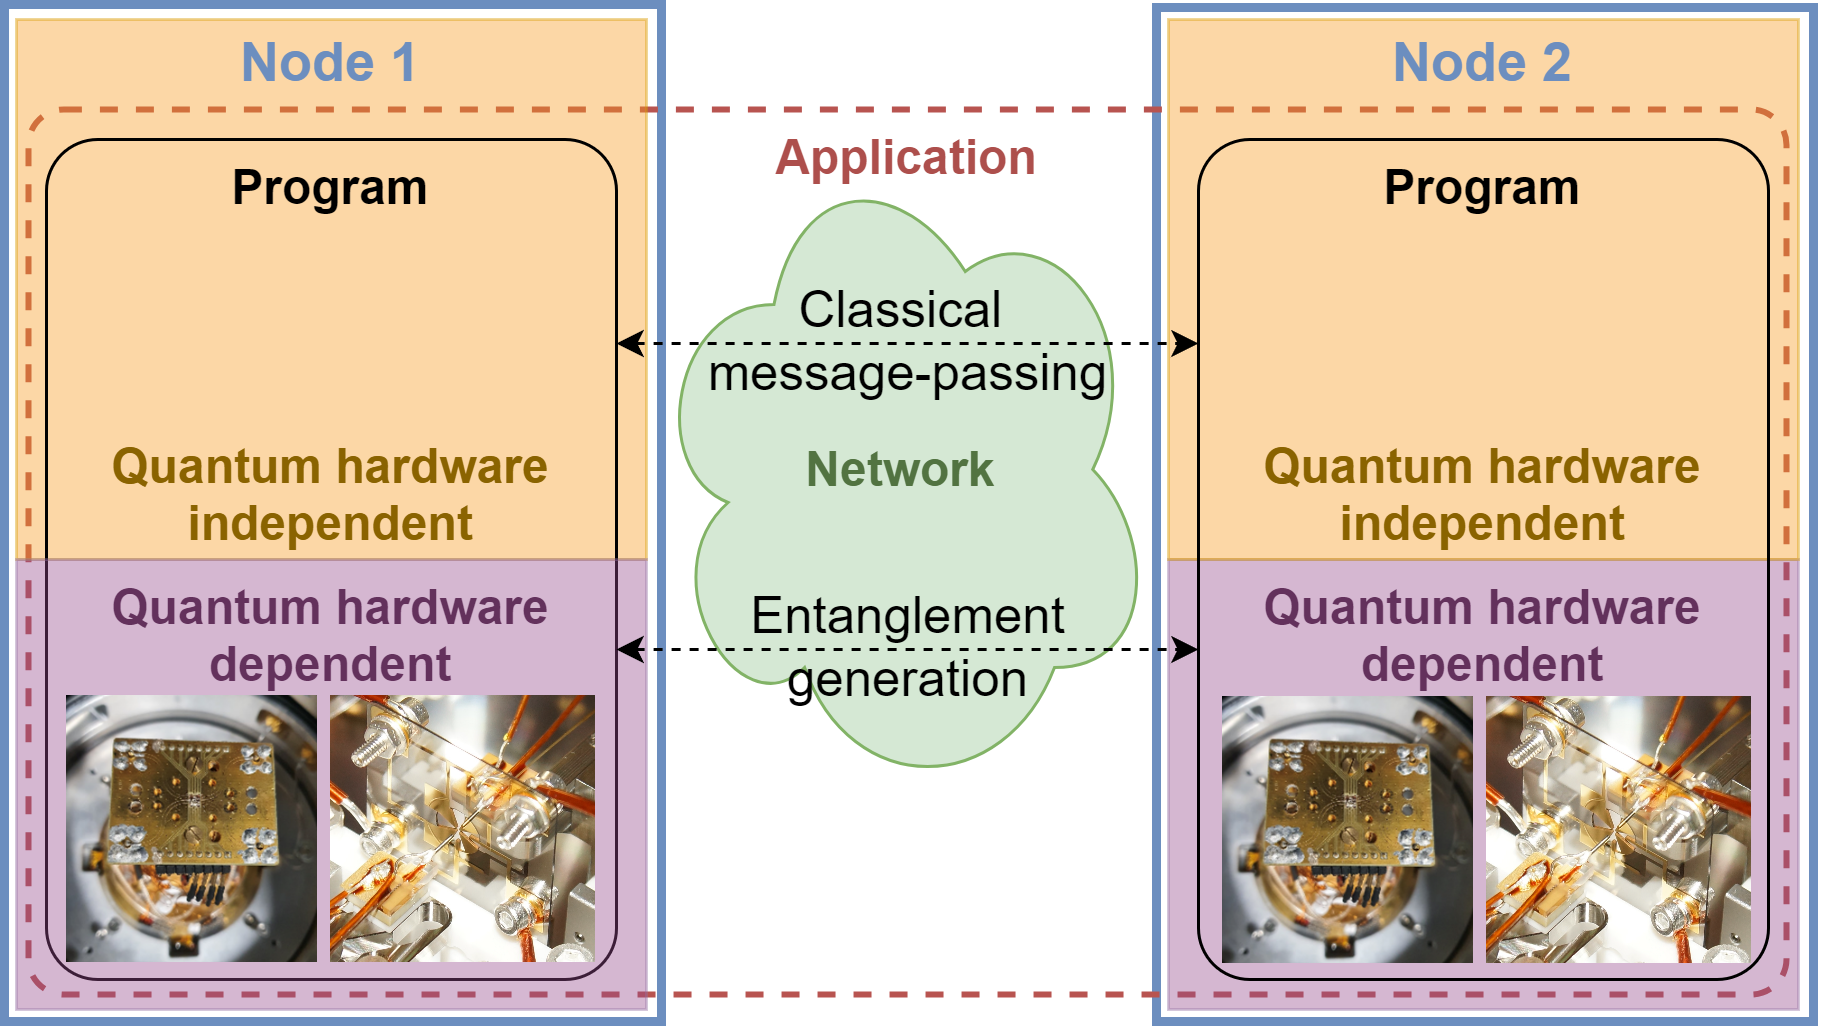
\includegraphics[width=1\linewidth]{figures/qnodeos/main/fig1/fig1.png}
\caption{\textbf{Application Paradigm.} A quantum networking application consists of multiple programs, each running on one of the end nodes~\cite{dahlberg_2022_netqasm} The distinct programs can only interact via (1) quantum communication (e.g. entanglement generation) and (2) classical communication. This allows a programmer to realize security-sensitive applications, but prohibits a global orchestration of the quantum execution, like one might do in (distributed) quantum computing~\cite{caleffi_distributed_2022} in which a single quantum program is executed on multiple nodes. Programs are written in high-level quantum hardware independent software, and executed on a quantum hardware independent system (our architecture) that controls a hardware dependent system (QDevice, \cref{qnodeos:fig:fig2}) such as a nitrogen-vacancy (NV) center node with a diamond chip (photo taken by authors, left images) or a trapped-ion quantum node~\cite{teller2023integrating} (right images). These platforms constitute physically very different QDevice systems, but can both be programmed by our architecture.}
\label{qnodeos:fig:fig1}
\end{figure}

\section{Design Considerations and Challenges}
\paragraph{Interactive Classical-Quantum Execution}
The execution of quantum network applications requires a continuing interaction between the quantum and classical parts of the execution, including interactions between different programs (\cref{qnodeos:fig:fig1}). For example, during secure quantum computing in the cloud~\cite{broadbent_2009_ubqc,ma_qenclave-practical_2022}, the program on the server is waiting for classical messages from a remote client before continuing the quantum execution at the server. This is in sharp contrast to quantum computing applications, where one quantum program can be executed in a single batch, without the need to keep quantum states live while waiting for input from other programs. In quantum computing, only relatively low-level interactions between classical and quantum processing are realized, such as in quantum error correction~\cite{lidar2013quantum}, or mid-circuit measurements~\cite{botelho_error_2022}. Higher-level classical-quantum interactions in quantum computing~\cite{bharti_noisy_2022} do not keep qubits live in memory.

We assume that the programs are divided into classical and quantum blocks of instructions (by a programmer or a compiler). Classical blocks consist of local classical operations executed on a conventional classical processor, as well as networked classical operations (i.e. sending messages to remote nodes) executed using network devices. Quantum blocks consist of local quantum operations (gates, measurements, classical control logic), as well as networked quantum operations (entanglement generation) executed on quantum hardware. A single quantum block, in essence, corresponds to a program in quantum computing, and may contain simple classical control logic, such as for the purpose of mid-circuit measurements~\cite{botelho_error_2022}.

\paragraph{Different Hardware Platforms}
Interfacing with different hardware platforms presents technological challenges: currently, a clear line between software and hardware has not been defined, and the low-level control of present-day quantum processor hardware has been built to conduct physics experiments. Early microarchitectures~\cite{bertels_quantum_2020,fu_2019_eqasm} and operating systems~\cite{giortamis_qos_2024,kong_2021_origin} for quantum computing do not address the execution of quantum network applications. We thus have to define a hardware abstraction layer (HAL), capable of interfacing with present-day quantum network setups. 

\paragraph{Timescales}
It is a fundamental challenge that different parts of such a system operate at vastly different timescales. For nodes separated by hundreds of kilometers, the duration of network operations is in the millisecond (ms) regime, and some applications~\cite{wehner_2018_stages} need  significant local classical processing (ms). In contrast, the time to execute quantum operations on processing nodes is in the regime of microseconds ($\mu$s), and the low-level control (including timing synchronization between neighboring nodes to generate entanglement~\cite{humphreys_2018_delivery}) requires nanosecond (ns) precision.

\paragraph{Memory Lifetimes}
Present-day quantum network nodes have short coherence times, posing a technological challenge to ensure operations are executed within the timeframe allowed by the quantum memory.

\paragraph{Scheduling Local and Network Operations}
In contrast to classical networking, entanglement is a form of stateful connection already at the physical layer where both nodes hold one qubit. Heralded entanglement generation requires agreement between neighboring network nodes to trigger entanglement generation in precise time-bins~\cite{dahlberg_2019_egp}, organized into a network schedule~\cite{skrzypczyk_2021_arch} that dictates when nodes make entanglement. It is a technological challenge to manage the interdependencies between the schedule of local operations, and the networked operations, since in all current processing node implementations~\cite{pompili_2021_multinode,drmota_robust_2023}, entanglement generation cannot be performed simultaneously with local operations~\cite{pompili_2021_multinode,krutyanskiy_light-matter_2019}. While interdependencies may be mitigated in the future~\cite{vardoyan_2022_netarch}, this implies that we cannot schedule (i.e. decide when to execute) the execution of local quantum operations independently of the network schedule.

\paragraph{Multitasking}
When executing quantum network applications, one node is typically idle while waiting for the other node before it can continue execution. It is hence a fundamental challenge how we can increase the utility of the system by performing multitasking~\cite{mccullough_design_1965-1,dennis_segmentation_1965}, that is, allowing the concurrent execution of several programs at once to make use of idle times. Consequently, there is a need for managing state and resources for multiple independent programs, including processes, quantum memory management, and entanglement requests. 

\begin{figure*}[htb]
\centering
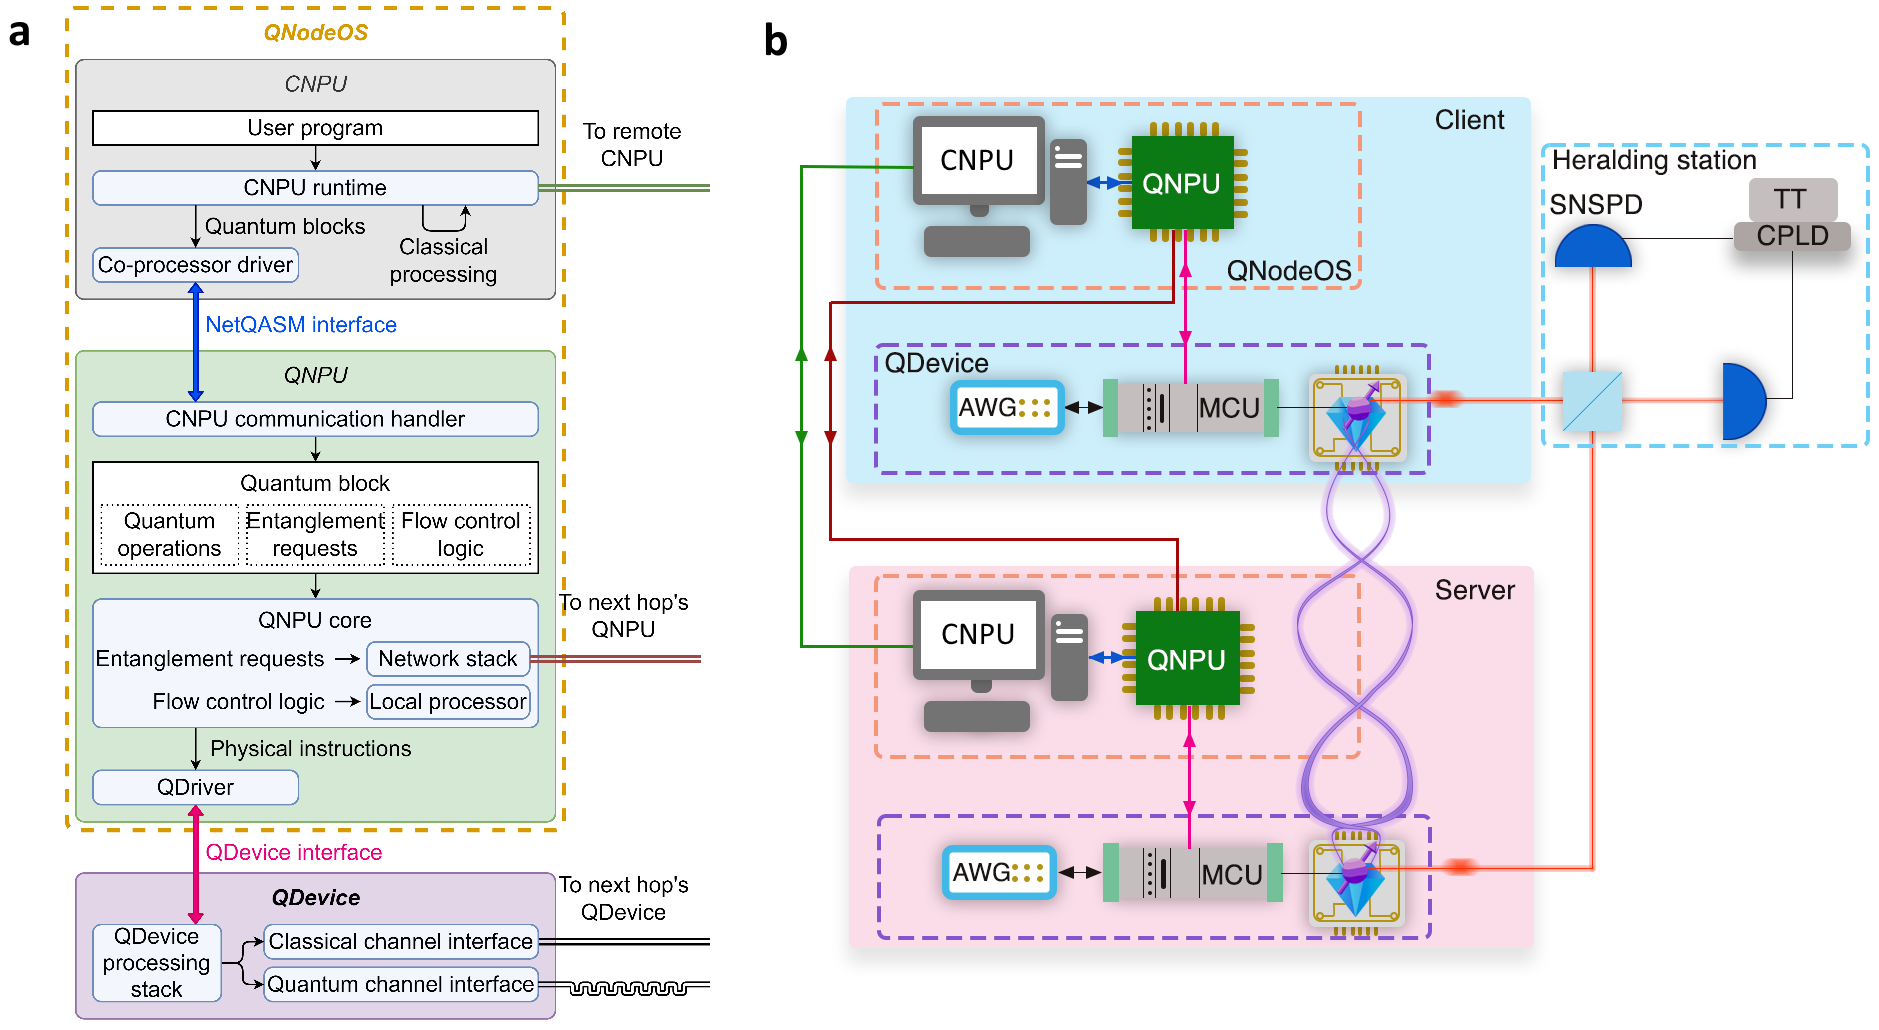
\includegraphics[width=1\linewidth]{figures/qnodeos/main/fig2/fig2.png}
\caption{\textbf{QNodeOS architecture.} \textbf{(a)} QNodeOS consists of a Classical Network Processing Unit (CNPU) and a Quantum Network Processing Unit (QNPU, classical system). QNodeOS controls a QDevice (quantum hardware and low-level classical control).
\textbf{(b)} Schematic of our implementation of QNodeOS on a two-node setup where both QDevices control a single qubit in a diamond nitrogen-vacancy (NV) center. The CNPU is implemented on a general-purpose PC, and the QNPU on an embedded system, connected via Gigabit Ethernet (blue). The QNPU connects to its QDevice via a serial peripheral interface (SPI, pink). The two QNPUs (brown), and the two CNPUS (green) connect to each other via Gigabit Ethernet. The setup is based on~\cite{pompili_2022_experimental} with two QDevices (including arbitrary waveform generators (AWG) and microcontroller units (MCU); QDevices communicating over a classical DIO interface) and a heralding station composed by a balanced 50:50 beam-splitter (whose output ports are connected to superconducting nanowire single-photon detectors (SNSPD) via optical fibers (red)),  a  TimeTagger (TT), and a \ac{CPLD} that heralds the entanglement generation between QDevices and sends a classical message to the MCU.}
\label{qnodeos:fig:fig2}
\end{figure*}

\section{Architecture}
\label{qnodeos:sec:architecture}
We divide the architecture logically into three main components (\cref{qnodeos:fig:fig2}, \cref{qnodeos:sec:methods}): The Classical Network Processing Unit (CNPU) is responsible for starting the execution of programs, and the execution of classical code blocks; the Quantum Network Processing Unit (QNPU) is responsible for governing the execution of the quantum code blocks; The CNPU and QNPU together form QNodeOS and control the QDevice, which is responsible for executing any quantum operations (gates, measurements, entanglement generation at the physical layer~\cite{dahlberg_2019_egp}) on the quantum hardware. Upon starting the execution the CNPU creates a corresponding CNPU process (a well-known concept in classical operating systems~\cite{dennis_programming_1966-1,tanenbaum_operating_2005}), registers the program on the QNPU (via the QNPU's end node application programming interface (API), \cref{qnodeos:sec:design:qnpu_stack}), which, in turn, creates its own associated QNPU process (including context such as process owner, ID, process state and priority). QNodeOS also defines kernel processes on the QNPU, which are similar to user processes, but are created when the system starts (on boot). The CNPU sends quantum blocks to the QNPU in the form of NetQASM subroutines~\cite{dahlberg_2022_netqasm}. Classical control logic in quantum blocks is executed by the QNPU processor. Quantum gates and measurements (from any QNPU process) and entanglement instructions (from the network process) are delegated to the QDevice by submitting physical instructions (\cref{qnodeos:sec:methods}), after which the QDevice responds back with the result of the instruction. 

To enable different hardware platforms, we introduce a QDriver realizing the HAL for any hardware corresponding to our minimal QDevice system model (\cref{qnodeos:sec:methods}). The QDriver is responsible for translating quantum operations, expressed in NetQASM~\cite{dahlberg_2022_netqasm}, into platform dependent (streams of) physical instructions to the underlying QDevice. We realize a QDriver for the trapped-ion system of~\cite{teller2023integrating,teller2021heating}, and one for NV centers in diamond based on the system of~\cite{hermans2022qubit,pompili_2021_multinode,pompili_2022_experimental}. We validate the trapped-ion QDriver (\cref{qnodeos:fig:fig5}) by implementing and verifying a set of single-qubit gate operations (\cref{qnodeos:sec:methods}), and the QDriver on the NV system as part of the full stack system evaluation (see below). 
To allow for different timescales, we logically divide the architecture into CNPU, QNPU and QDevice which can thus be realized at different timing scale granularities. In our proof-of-concept implementation, we realize the CNPU and QNPU on different devices, reflecting the ms timescales of communication between distant nodes (\cref{qnodeos:sec:methods}).

Ensuring the necessary interactivity requires architectural as well as implementation choices: as programs may depend on messages from remote nodes, the architecture needs to be able to dynamically handle both classical and quantum blocks, even if not known at runtime. Consequently, it is not possible to preload all quantum blocks of the program into the low-level controller of the QDevice ahead of time as done in previous physics experiments. Instead, in our system model the QDevice is capable of executing individual physical instructions similar to a classical CPU. Consequently, the QNPU is continuously ready to receive new NetQASM subroutines from the CNPU, and the QDevice can continuously receive and respond to physical instructions from the QNPU (\cref{qnodeos:sec:methods}).

In our NV QDevice implementation, we address the challenge of interactivity by interleaving specific preloaded pulse sequences (realizing physical instructions sent from QNodeOS) and dynamical decoupling (DD) sequences (protecting quantum memory from decoherence) in an arbitrary waveform generator (AWG)~\cite{zurich_instruments_hdawg_2019}. The DD sequences extend qubit coherence times up to $T_{\text{coh}} = 13(2)$ ms, while arbitrary physical instructions can be handled by triggering the corresponding pulse sequence, without knowing them in advance (\cref{qnodeos:sec:methods}).

To integrate local operations with the network schedule, our architecture first introduces a QNPU scheduler that can choose which of the ready processes is assigned to the local processor (\cref{qnodeos:fig:fig2}) and QDevice. This allows interleaving the execution of different processes directly on the QNPU without incurring delays on the timescale of the CNPU (ms), addressing the challenge of short coherence times. In our implementation, we choose to schedule QNPU processes using a priority based non-preemptive scheduler~\cite{liu_1973_scheduling}, due to limited quantum memory lifetimes, which make it undesirable to pre-empt and temporarily store quantum states while halting the execution. Second, we realize a network process as a kernel process, which manages entanglement generation using the network stack~\cite{dahlberg_2019_egp,kozlowski_2020_qnp} (implemented in~\cite{pompili_2022_experimental} without the ability to execute network applications), including a network schedule that can be determined by a time-division multiple access (TDMA) controller~\cite{skrzypczyk_2021_arch}. The network process handles entanglement requests submitted by user processes, coordinates entanglement generation with the rest of the network via the TDMA controller, interacts with the QDevice and eventually returns entangled qubits to user processes. User processes enter the waiting state when they need entanglement, and become ready again once entanglement was delivered. The network process has the highest scheduling priority, and is consequently given precedence over the execution of any local quantum operations. We remark local operations may still be executed during time-bins already occupied by the network schedule, if a running non-preemptable user process prevents the network process from running, as we indeed observe in our evaluation.

To increase utility, QNodeOS allows multiple programs to be run concurrently, using the QNPU scheduler from above to enable multitasking~\cite{mccullough_design_1965-1,dennis_segmentation_1965} user processes on the QNPU itself. The QNPU hence needs to keep context for each process, including a virtual quantum memory space (as in classical operating systems~\cite{daley_virtual_1968-1}). Similar to classical memory management systems~\cite{peterson_operating_1985}, a quantum memory management unit (QMMU) on the QNPU manages qubit allocations from processes, and translates virtual qubit addresses in NetQASM subroutines to physical addresses in the QDevice. This allows flexibility in translating a virtual qubit address to: (1) a different physical qubit address over time, allowing qubits to be rearranged transparently in the physical memory in the future, or (2) a logical qubit address, when QNodeOS is executed on top of a processor employing quantum error correction~\cite{lidar2013quantum}. Entanglement generation between different pairs of processes at remote nodes are distinguished by Entanglement Request (ER) sockets, inspired by classical sockets~\cite{chesson_network_1975-1,leach_architecture_1983}, which are established once a user process requests entanglement from the network process. In our implementation, processes of the same priority are scheduled first-come-first-served~\cite{peterson_operating_1985}, where the total schedule of the program in our implementation is dependent both on the schedule on the CNPU as well as the QNPU (\cref{qnodeos:sec:methods}).

\begin{figure*}[htbp]
\centering
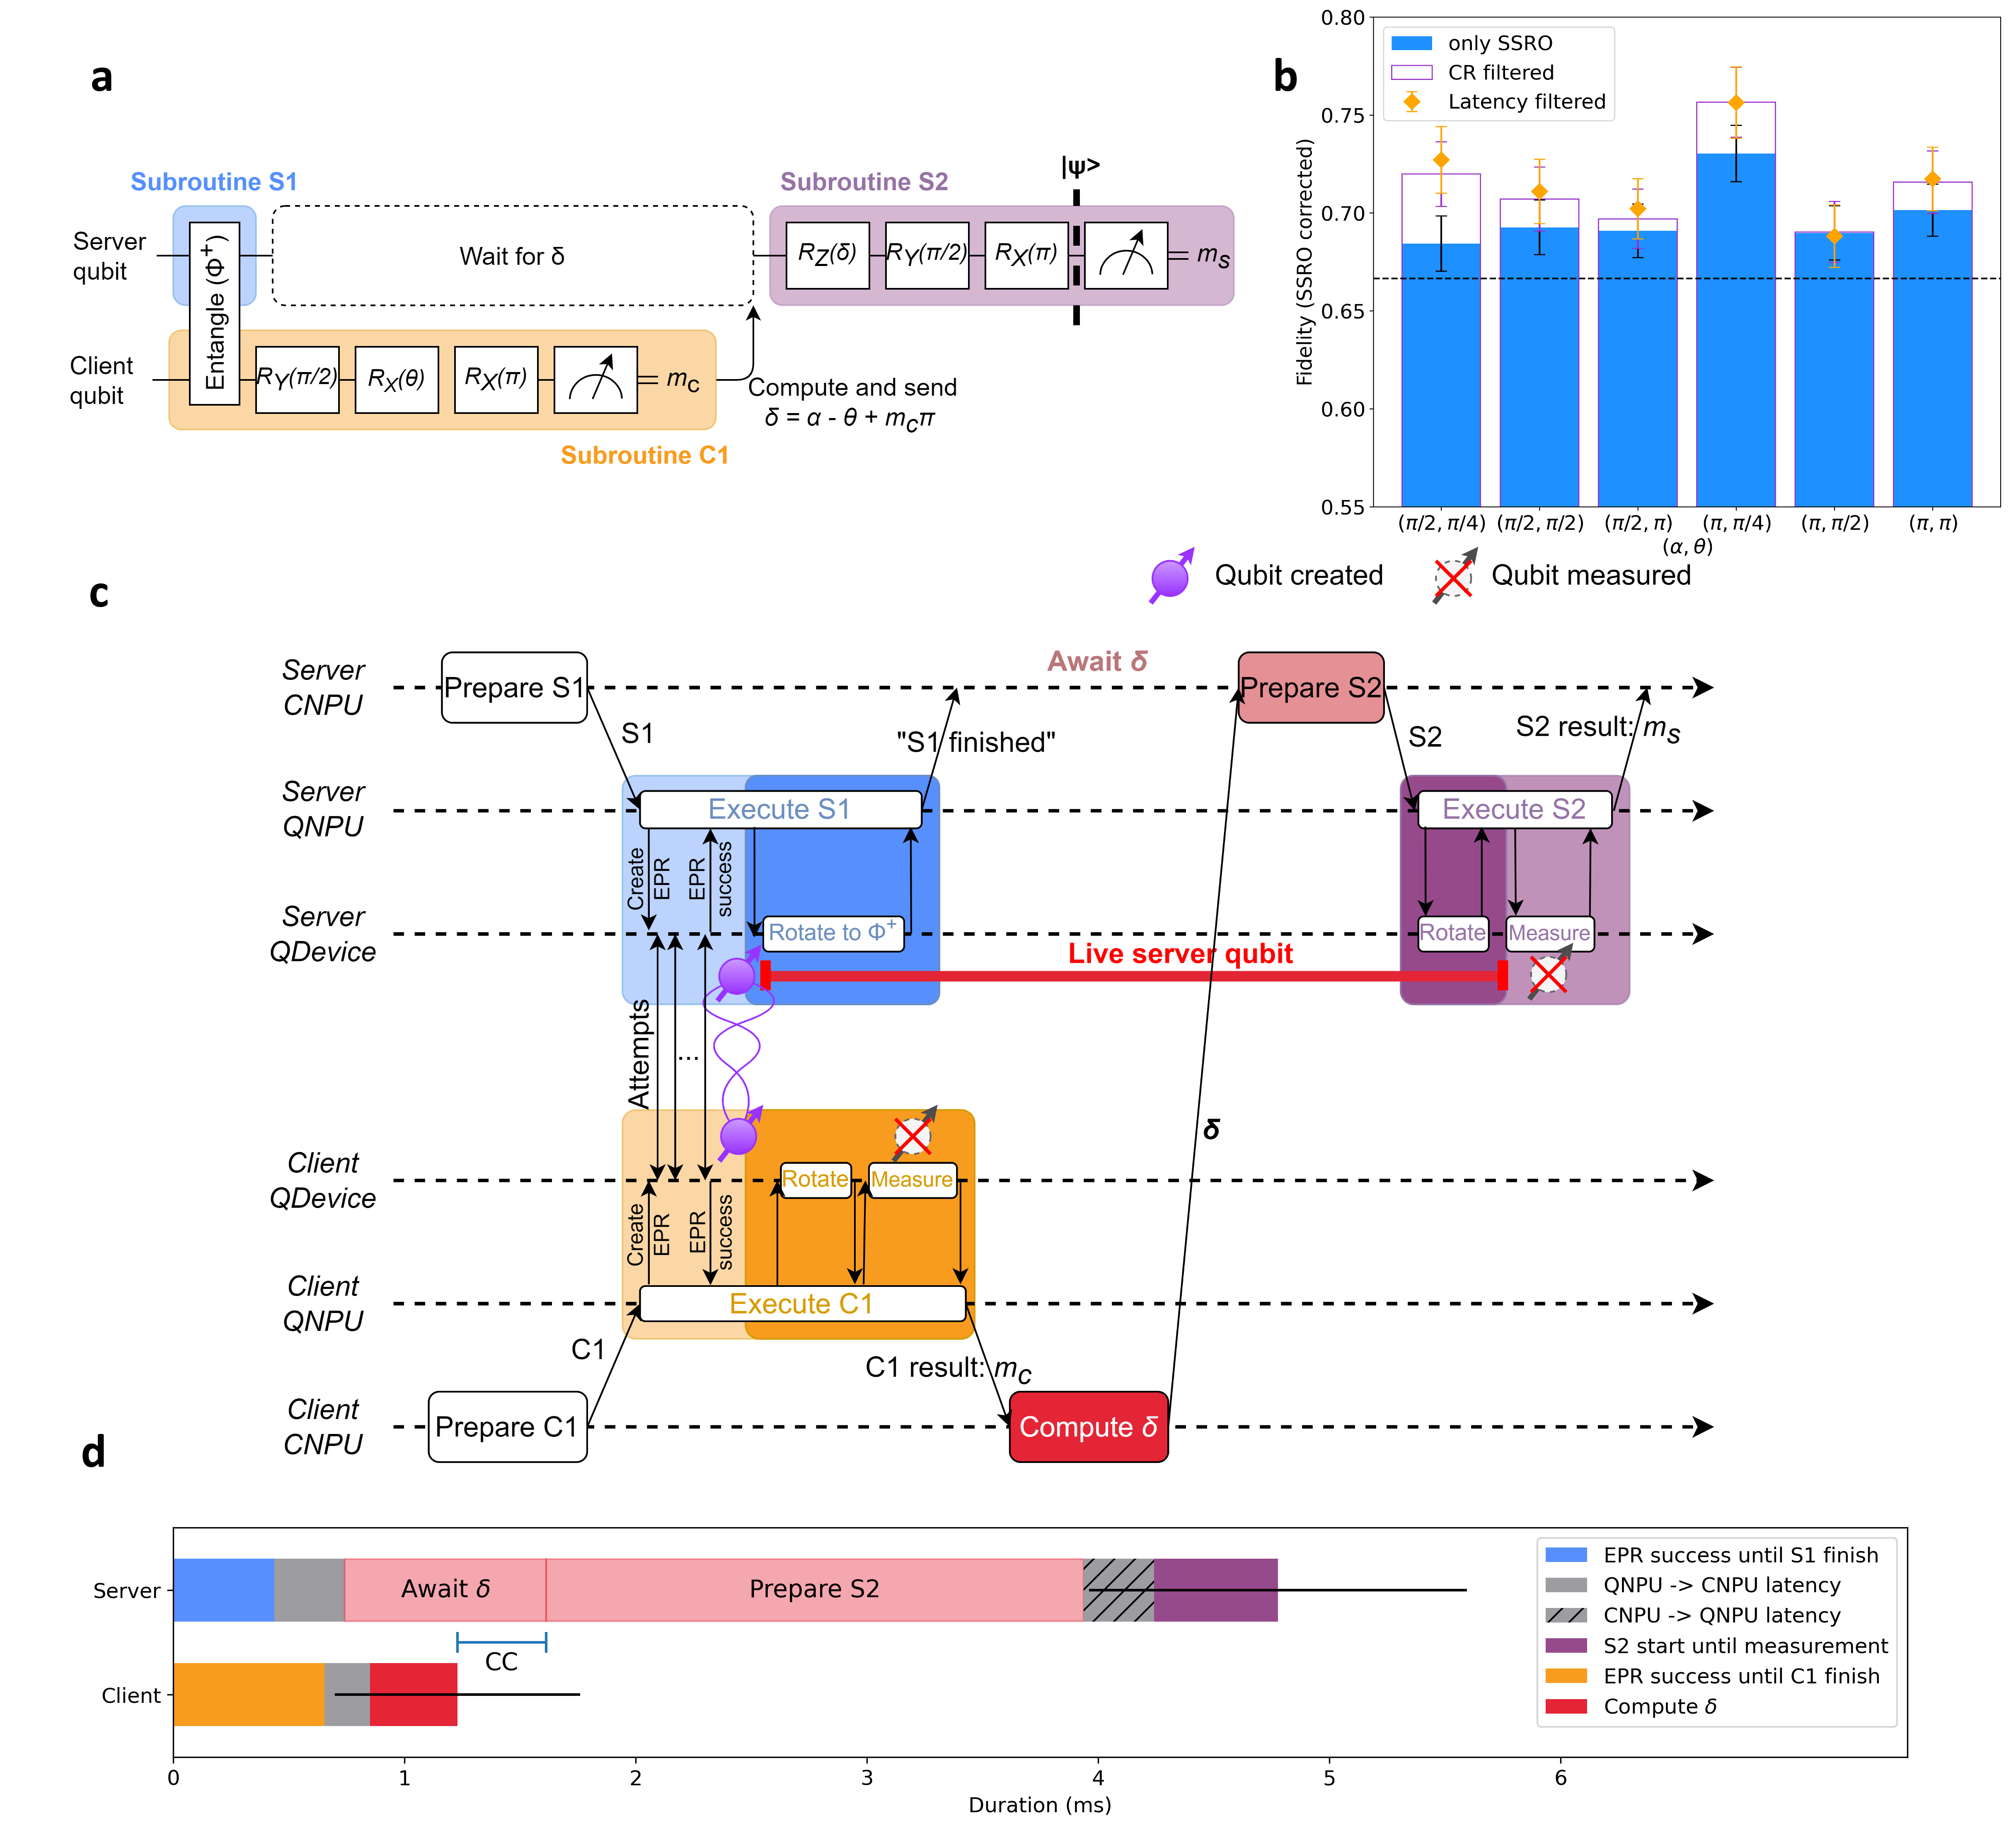
\includegraphics[width=0.89\linewidth]{figures/qnodeos/main/fig3/fig3.png}
\caption{\textbf{Delegated computation between two NV center nodes using QNodeOS.} 
\textbf{(a)} Delegated Quantum Computation (DQC) circuit (effective computation: single-qubit rotation $R_Z (\alpha)$, \cref{qnodeos:sec:methods}). The DQC application consists of $k$ repetitions of this circuit (varying measurement bases for tomography on $\ket{\psi}$) realized by two programs: the DQC-client program (client node, repeating the sequence ``quantum block (C1, orange) – classical block (computing $\delta$)'' $k$ times), and the DQC-server program (server node, repeating ``quantum block (S1, blue) - classical block (receiving $\delta$) – quantum block (S2, purple)'' $k$ times). Client and server produce an entangled pair $\ket{\Phi^+} = (\ket{00} + \ket{11}) / \sqrt{2}$ (S1 and first part of C1). The client performs local gates and a measurement (``destroying'' qubit), resulting in outcome bit $m_c$ (rest of C1). Client computes $\delta$ as function of $m_c$ and DQC parameters $\alpha \in [0,2\pi)$ and $\theta \in [0, 2\pi)$, and sends $\delta$ to server (classical message). Meanwhile the server keeps its qubit coherent (alive). Upon receiving $\delta$, the server applies gates depending on $\delta$, resulting in single-qubit state $\ket{\psi}$ (S2) depending only on $\alpha$ and $\theta$.
\textbf{(b)} Experimental results of executing DQC for 6 different sets of $(\alpha, \theta)$ parameters ($k=1200$, i.e. 7200 executions of the circuit of~\ref{qnodeos:fig:fig3}a). The fidelity of the resulting server state to the target state $\ket{\psi}$ is estimated using single-qubit tomography (1200 measurement results per data point), and corrected for known tomography errors (SSRO, blue), and post-selected for Charge-Resonance (CR) check validation (purple), and post-selected for latencies (orange) (\cref{qnodeos:sec:methods}).
\textbf{(c)} Sequence diagram including the interaction CNPU-QNPU-QDevice for one execution of the DQC circuit of \ref{qnodeos:fig:fig3}a on QNodeOS (repeated $k=1200$ times in each experiment) (time flows to the right; not to scale). CNPUs prepare NetQASM subroutines (C1, S1, S2), and send them to their respective QNPUs. CNPUs also do classical computation (computing $\delta$) and communication (message containing $\delta$). QNPUs execute subroutines, sending physical instructions to their QDevices. Entanglement is generated by QDevices doing a batch of attempts, resulting in the heralding of a two-qubit entangled state (Bell pair) rotated to $\ket{\Phi^+}$ by the server.
\textbf{(d)} Processing times and latencies while server qubit is live (time frame red line 3c, averaged over all 7200 circuit executions except executions with latency spikes, see~\cref{qnodeos:sec:methods}), including CNPU-QNPU communication latencies, CNPU processing on both nodes and client-server communication latency (CC) (average total of $\sim 4.8 (\pm 0.8)$ ms, error bars for the sum of individual segments (variance per segment in~\cref{qnodeos:sec:processing_time_latencies}).}
\label{qnodeos:fig:fig3}
\end{figure*}


\section{Demonstrations}
\paragraph{Delegated Computation}
We first validate our architecture and implementation by the first successful execution of an arbitrary – i.e. not preloaded – execution of a quantum network application in high-level software on quantum processors. We implement QNodeOS on a two-node setup of NV centers using one qubit per node (\cref{qnodeos:fig:fig2}, \cref{qnodeos:sec:methods}). We choose to execute an elementary form of delegated quantum computation (DQC)~\cite{broadbent_2009_ubqc} from a client to a server, because the client and server programs jointly realize repetitions of a circuit (\cref{qnodeos:fig:fig3}a) that triggers all parts of our system (\cref{qnodeos:fig:fig3}c). 
We first verify that the quantum result (fidelity) was found to be above the classical bound~\cite{massar_optimal_1995} $> 2/3$, which verifies that QNodeOS can successfully handle interactive applications consisting of entanglement generation, millisecond-scale memory lifetimes, and classical message passing. The non-perfect fidelity (\cref{qnodeos:fig:fig3}b) comes mainly from two sources: a noisy entangled state with fidelity 0.72(2) (quantum hardware limitation), and decoherence in the server qubit (depending on $T_{\text{coh}}$) due to waiting for several milliseconds (classical software latencies, \cref{qnodeos:fig:fig3}d).
We proceed to characterize latencies. As expected, we find that the duration that the server qubit must remain alive is dominated (> 50\%) by processing in the CNPU, which could be improved by caching the preparation of S2, and implementing the CNPU and QNPU on one board (Outlook). We observe that CNPU processing time varies significantly (standard deviation 30\%, \cref{qnodeos:sec:processing_time_latencies}), due to limited scheduling control over CNPU processes (\cref{qnodeos:sec:methods}).  Using an a priori estimate of what delays lead to too low a quality of execution (i.e. delays that are too long for the server qubit to be stored with sufficiently high quality), we discard application iterations in which the CNPU latencies spiked by more than 8.95 ms. This lead the discarding of 2\% of iterations in post-processing (\cref{qnodeos:sec:methods}).

\paragraph{Demonstration of Multitasking}
We also validate QNodeOS's multitasking capability by the first concurrent execution of two quantum applications on a quantum network: the DQC application, and a single-node local gate tomography (LGT) application on the client (\cref{qnodeos:fig:fig4}a). The two programs for the client are started in the CNPU at the same time (two CNPU processes, subject to CNPU scheduler), which means that the QNPU continuously receives subroutines for both programs from the CNPU (two QNPU processes and corresponding subroutines, subject to QNPU scheduler). This leads to a multitasking challenge directly on the QNPU to schedule the different subroutines received (\cref{qnodeos:fig:fig4}b). Since the client has only one qubit, the multitasking of DQC and LGT never results in both programs having a quantum state alive on the client; therefore, multitasking should not affect the fidelity of LGT. We observe interleaved execution of DQC quantum blocks and LGT quantum blocks on the client node (\cref{qnodeos:fig:fig4}b). The LGT application produces a quantum result (fidelity, \cref{qnodeos:fig:fig4}c) equal to that in the scenario where we run LGT on its own (not interleaved by DQC circuit executions), as expected.

We further test multitasking by scaling up the number of programs executed concurrently, up to 5 DQC and 5 LGT programs running on the client at the same time. The interleaved execution of subroutines of different programs increases device utilization (fraction of time spent on executing physical instructions) on the client QDevice compared to the same scenario but with multitasking disabled (\cref{qnodeos:fig:fig4}d). As expected, we observe that LGT subroutines were scheduled to be executed in between DQC subroutines, resulting in lower client QDevice idle time. When multitasking 1 DQC and 1 LGT program, we observe 1 or 2 subroutines in between DQC iterations in most cases (LGT subroutine duration ~2.4 ms, \cref{qnodeos:sec:multitasking-scaling}). We observe cases where both server and client QDevice remain idle, which could be improved in part by smarter CNPU-QNPU scheduling algorithms: (1) both the client and server wait until the start of the next network schedule time-bin (time-bin length 10 ms) (2) the client QNPU finishes a subroutine for user process P, but must wait until the CNPU sends the next subroutine for P (up to 150 ms for 1 DQC and 1 LGT program, but less (up to only 8 ms) when more applications are running, since there are more CNPU processes independently submitting subroutines), (3) the client is ready to perform entanglement generation for DQC, but the next time-bin starts only at some future time $t$, preventing activation of the network process. The scheduler activates a user process which runs a LGT circuit, which completes at some time $>t$, delaying the start of the DQC network process, even though the server node was ready at $t$.

\begin{figure*}[htbp]
\centering
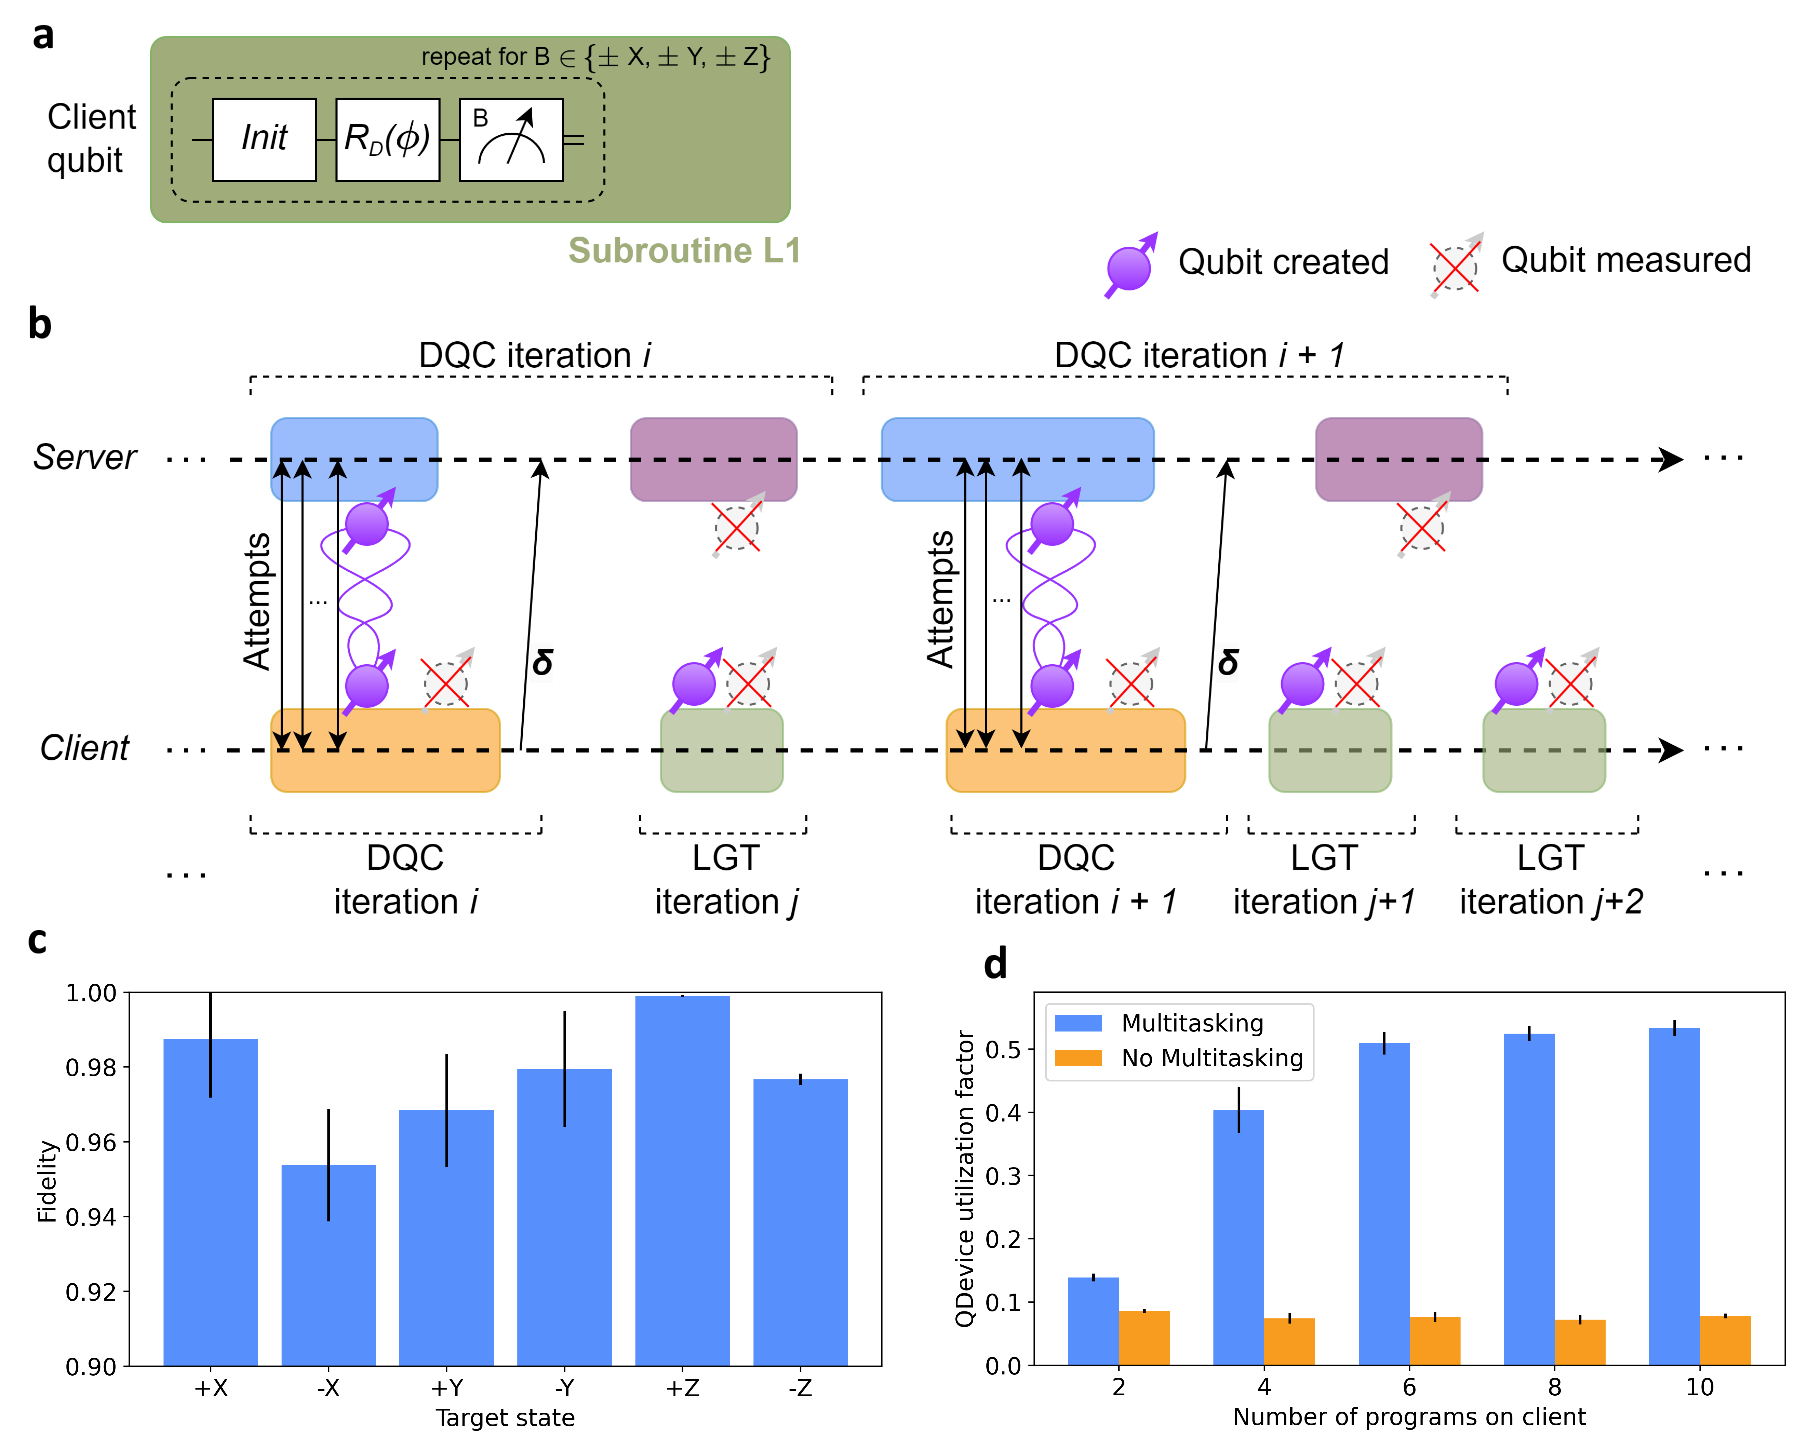
\includegraphics[width=0.95\linewidth]{figures/qnodeos/main/fig4/fig4.png}
\caption{\textbf{Multitasking experiment on two NV centers with QNodeOS}.
\textbf{(a)} Local Gate Tomography (LGT) Circuit. A single NetQASM subroutine (L1) executes the following 6 times for different bases $B \in \{\pm X, \pm Y, \pm Z\}$: initialize qubit to $\ket{0}$, rotate around fixed axis $D \in \{X,Y\}$ by angle $\ket{\phi}$, measure in $B$. The LGT application consists of a single LGT program, which submits subroutine L1 for execution to the QNPU (fixed $D$ and $\phi$) $k$ times in succession.
\textbf{(b)} Example sequence diagram illustrating concurrent execution (multitasking) of the DQC application (\cref{qnodeos:fig:fig3}) and the LGT program on the client: time slice in which two DQC circuit repetitions (\cref{qnodeos:fig:fig3}a) are realized (2 subroutines on the client (orange), 4 on the server (blue and purple)), and three LGT circuit repetitions (3 subroutines, green). The client QNPU receives subroutines for both the DQC program and the LGT program, which the QNPU scheduler can interleave: While the server executes S2 (purple), the client cannot yet execute the next S1 (orange) since it involves joint entanglement generation. In this idle time, the client can execute a number of LGT subroutines (number can vary).
\textbf{(c)} Results of multitasking LGT (client) and DQC (on both server and client). For each input pair $(D, \phi) \in \{ (X,0), (X,\pi), (Y,pi/2), (Y,-\pi/2), (X,-\pi/2), (X,\pi/2) \}$ (6 cardinal states $\{\pm X, \pm Y, \pm Z\}$), the following experiment was performed: simultaneously (1) a single LGT program was initiated on the client ($k=1000$), (2) a single DQC-client program was initiated on the client ($k=200$ successive subroutines), and (3) a single DQC-server program was initiated at the server ($k=200$, i.e. 400 successive subroutines). This resulted in a total of 6000 LGT subroutine executions and 36000 LGT measurement results, yielding plotted fidelity estimates for the LGT quantum state before measurement. Results are the same as running LGT on its own (no multitasking with DQC), as expected (\cref{qnodeos:sec:multitasking-tomography}).
\textbf{(d)} Scaling number of programs on the client. For $N \in \{1,2,3,4,5\}$, we initiate at the same time: (1) $N$ LGT programs (each using $k=100$) on the client, (2) N DQC-client programs on the client (each using $k=60$), and (3) $N$ DQC-server programs on the server (each using $k=60$). This results in $2N$ programs active at the same time on the client, each continuously submitting subroutines from the CNPU to the QNPU, where the QNPU scheduler chooses which process to execute when. Each experiment was repeated but with multitasking disabled on the client. Plot shows the utilization factor of the QDevice (fraction of time spent executing instructions), corrected for variable entanglement generation duration (\cref{qnodeos:sec:methods}), with (blue) and without (orange) multitasking, showing that multitasking can increase device utilization.}
\label{qnodeos:fig:fig4}
\end{figure*}

\section{Outlook}
We designed and implemented the first architecture allowing high-level programming and execution of quantum network applications. To deploy our system onto nodes separated by several kms it would be desirable to merge both the CNPU and the QNPU onto one system board, ideally with mutual access to a shared memory to avoid ms delays in their communication. Such a merge would also allow the definition of a joint classical-quantum executable and processes, opening further doors to reduce latencies by a better scheduling control.

Our work provides a framework for a new domain of computer science research into programming quantum network applications on quantum processors including: novel real-time~\cite{ramamritham_scheduling_1994} scheduling algorithms for classical-quantum processes, compile methods for quantum network applications, or novel programming language concepts including entanglement to make software development even easier, thus advancing the vision to make quantum network technology broadly available.


\begin{figure}[htb]
\centering
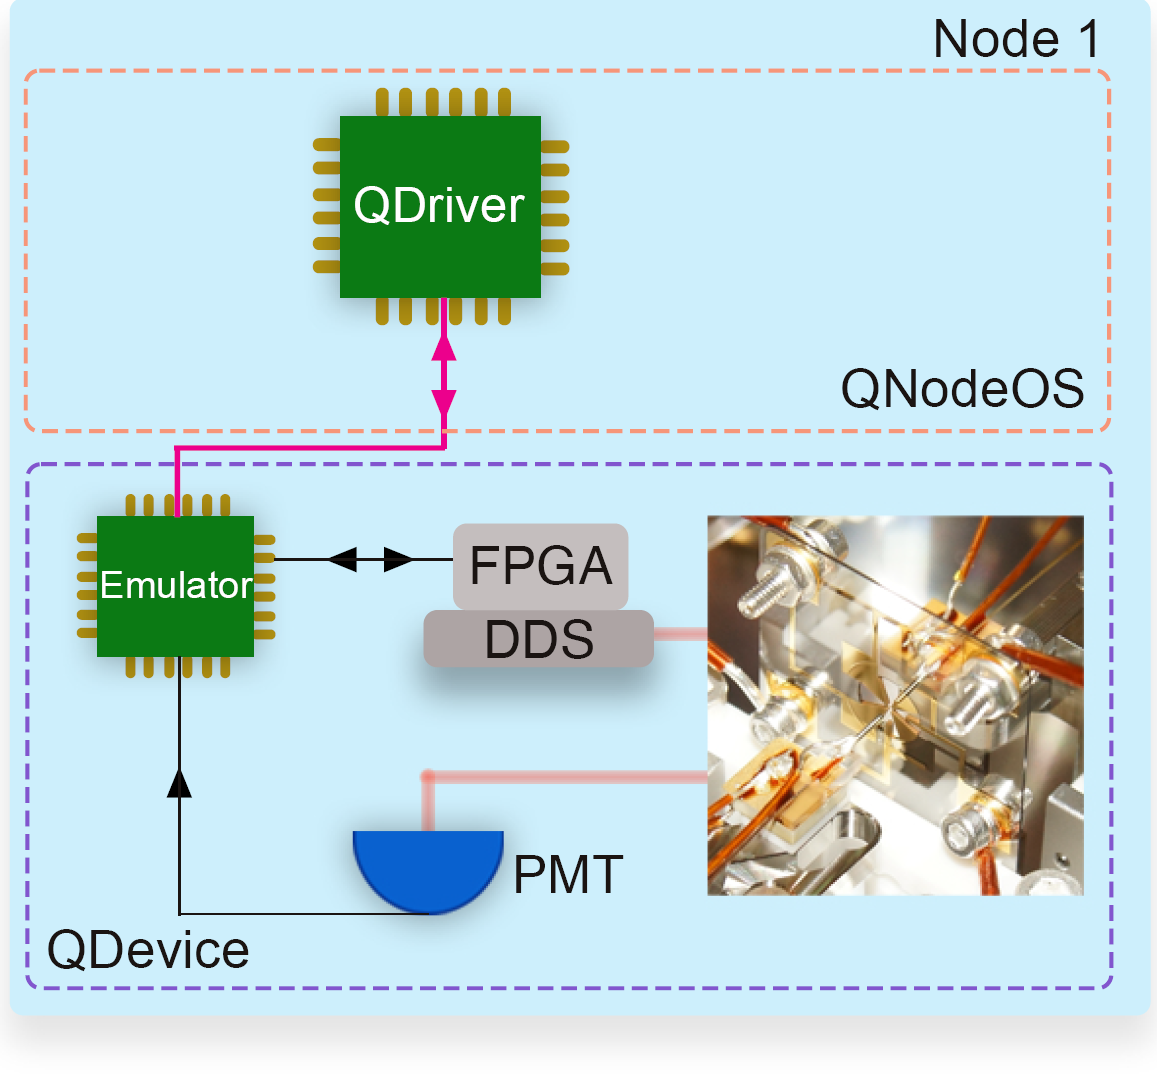
\includegraphics[width=1\linewidth]{figures/qnodeos/main/fig5/fig5.png}
\caption{\textbf{Trapped-ion QDevice implementation.} Schematic of our implementation of QNodeOS on a single-node setup in which the QDevice contains a single trapped-ion qubit. The QNPU QDriver is implemented on a field-programmable gate array (FPGA) that connects to its QDevice via a serial peripheral interface (SPI) (\cref{qnodeos:sec:methods}). The setup consists of an emulator that translates between SPI messages and TTL signals, experimental control hardware that includes an FPGA and direct digital synthesis (DDS) modules, a trapped-ion qubit~\cite{teller2023integrating} under ultra-high vacuum (\cref{qnodeos:fig:fig1}), and a photomultiplier tube (PMT) that registers atomic fluorescence.}
\label{qnodeos:fig:fig5}
\end{figure}
\section{Methods}
\label{qnodeos:sec:methods}

\paragraph{QDevice Model}

The QDevice includes a physical quantum device, which can initialize and store quantum bits (qubits) which are individually identified by a physical address, apply quantum gates, measure qubits, and create entanglement with QDevices on other nodes (either entangle-and-measure, or entangle-and-keep~\cite{dahlberg_2019_egp}). The QDevice exposes the following interface to QNodeOS (\cref{qnodeos:sec:appendix-qdevice}): number of qubits available, and the supported physical instructions that QNodeOS may send. Physical instructions include qubit initialization, single- and two-qubit gates, measurement, entanglement creation, and a `no-op' for do nothing. Each instruction has a corresponding response (including entanglement success or failure, or a measurement outcome) that the QDevice sends back to QNodeOS.

QNodeOS and the QDevice interact by passing messages back and forth on clock ticks at a fixed rate (100 kHz in our NV implementation, 50 kHz in the trapped-ion implementation). During each tick, at the same time (1) QNodeOS sends physical instruction to QDevice, (2) QDevice can send a response (for a previous instruction). Upon receiving an instruction, the QDevice performs the appropriate (sequence of) operations (e.g. a particular pulse sequence in the AWG). An instruction may take multiple ticks to complete, where the QDevice returns the response (success, fail, outcome) during the first clock tick following completion. The QDevice handles an entanglement instruction by performing (a batch of) entanglement generation attempts~\cite{pompili_2022_experimental} (synchronized by the QDevice with the neighboring node's QDevice). 

\paragraph{QNodeOS Architecture}

QNodeOS consists of two layers: CNPU and QNPU (\cref{qnodeos:fig:fig2}a, \cref{qnodeos:sec:architecture}, Supplementary). Processes on the QNPU are managed by the Process Manager, and executed by the local processor. Executing a user process means executing NetQASM~\cite{dahlberg_2022_netqasm} subroutines (quantum blocks) or that process, which involves running classical instructions (including flow control logic) on the QNPU's local processor, sending entanglement requests to the network stack, and handling local quantum operations by sending physical instructions to the QDriver (\cref{qnodeos:fig:fig2}a). Executing the network process means asking the network stack which request (if any) to handle and sending the appropriate (entanglement generation) instructions to the QDevice. 

A QNPU process can be in the following states (\cref{qnodeos:fig:process-states} in Supplementary for state diagram): idle, ready, running and waiting. A QNPU process is running when the QNPU processor is assigned to it. The network process becomes ready when a network schedule time-bin starts; it becomes waiting when it finished executing and waits for the next time-bin; it is never idle. A user process is ready when there is at least one NetQASM subroutine pending to be executed; it is idle otherwise; it goes into the waiting state when it requests entanglement from the network stack (using NetQASM entanglement instructions~\cite{dahlberg_2022_netqasm}) and is made ready again when the requested entangled qubit(s) are delivered. 

The QNPU scheduler oversees all processes (user and network) on the QNPU, and chooses which ready process is assigned to the QNPU processor. CNPU processes can run concurrently, and their execution (order) is handled by the CNPU scheduler. The QNPU scheduler operates independently and only acts on QNPU processes. CNPU processes can only communicate with their corresponding QNPU processes. Since multiple programs can run concurrently on QNodeOS, the QNPU may have multiple user processes that have subroutines waiting to be executed at the same time. This hence requires scheduling on the QNPU.

Processes allocate qubits through the Quantum Memory Management Unit (QMMU), which manages virtual qubit address spaces for each process, and translates virtual addresses to physical addresses in the QDevice. The QMMU can also transfer ownership of qubits between processes, for example from the network process (having just created an entangled qubit), to a user process that requested this entanglement. The Network Stack uses Entanglement Request (ER) sockets (opened by user programs through QNPU API once execution starts) to represent quantum connections with programs on other nodes. The Entanglement Management Unit (EMU) maintains all ER sockets and makes sure that entangled qubits are moved to the correct process.

\paragraph{NV QDevice Implementation}

The two-node network employed in this work includes the nodes “Bob” (server) and “Charlie” (client) (separated by 3 meters) described in~\cite{pompili_2021_multinode,hermans2022qubit,pompili_2022_experimental}. For the QDevice, we replicated the setup used by~\cite{pompili_2022_experimental}, which mainly consists of: an Adwin-Pro II~\cite{adwin} acting as the main orchestrator of the setup; a series of subordinate devices responsible for qubit control, including laser pulse generators, optical readout circuits and an arbitrary waveform generator (Zurich Instruments HDAWG~\cite{zurich_instruments_hdawg_2019}). The quantum physical device, based on NV centers, counts one qubit for each node. The two QDevices share a common 1 MHz clock for high-level communication and their AWGs are synchronized at sub-nanosecond level for entanglement attempts.

We address the challenge of limited memory lifetimes by employing dynamical decoupling (DD).  While waiting for further physical instructions to be issued, DD sequences are used to preserve the coherence of the electron spin qubit~\cite{de_lange_universal_2010}. DD sequences for NV-centers can prolong the coherence time ($T_{\text{coh}}$) up to hundreds of ms~\cite{hermans2022qubit} or even seconds~\cite{abobeih_2018_one_sec}. In our specific case, we measured $T_{\text{coh}}$=13(2) ms for the server node, corresponding to ~1300 DD pulses. The discrepancy to the state-of-the-art for similar setups is due to several factors. To achieve such long $T_{\text{coh}}$, a thorough investigation of the nuclear spin environment is necessary to avoid unwanted interactions during long DD sequences, resulting in an even more accurate choice of interpulse delay. Other noise sources include unwanted laser fields, the quality of microwave pulses and electrical noise along the microwave line.  

A specific challenge arises at the intersection of extending memory lifetimes using DD, and the need for interactivity: to realize individual physical instructions, many waveforms realizing are uploaded to the Arbitrary Waveform Generator (AWG), where the QDevice decodes instructions sent by QNodeOS into specific preloaded pulse sequences. This results in a waveform table, containing 170 entries. The efficiency of the waveforms is limited by the AWG's waveform granularity that corresponds to steps that are multiples of 6.66 ns, having a direct impact on the $T_{\text{coh}}$. We are able to partially overcome this limitation through the methods described in~\cite{corna_efficient_2021}. Namely, each preloaded waveform, corresponding to one single instruction, has to be uploaded 16 times in order to be executed with sample precision. To not fill up the waveform memory of the device, we apply the methods in~\cite{corna_efficient_2021} only to the DD pulses that are played while the QDevice waits for an instruction from the QNPU, whereas the instructed waveforms (gate/operation + first block of XY8 DD sequence) are padded according to the granularity, if necessary.
The physical instructions supported by our NV QDevice is given in~\cref{qnodeos:sec:qdevice-nv}.

\paragraph{NV QNPU Implementation}

The QNPUs for both nodes are implemented in C++ on top of FreeRTOS~\cite{freertos}, a real-time operating system for microcontrollers. The stack runs on a dedicated MicroZed~\cite{microzed}---an off-the-shelf platform based on the Zynq-7000 SoC, which hosts two ARM Cortex-A9 processing cores, of which only one is used, clocked at 667 MHz. The QNPU was implemented on top of FreeRTOS to avoid re-implementing standard OS primitives like threads and network communication. FreeRTOS provides basic OS abstractions like tasks, inter-task message passing, and the TCP/IP stack. The FreeRTOS kernel---like any other standard OS---cannot however directly manage the quantum resources (qubits, entanglement requests and entangled pairs), and hence its task scheduler cannot take decisions based on such resources. The QNPU scheduler adds these capabilities (\cref{qnodeos:sec:qnpu_impl_scheduler}).

The QNPU connects to peer QNPUs via TCP/IP over a Gigabit Ethernet interface (IEEE 802.3 over full-duplex Cat 5e). The communication goes via two network switches (Netgear JGS524PE, one per node). The two QNPUs are time-synchronized through their respective QDevices (granularity 10 $\mu$s), since these already are synchronized at the $\mu$s-level (common 1Mhz clock).

The QNPU interfaces with the QDevice's ADwin-Pro II through a 12.5 MHz SPI interface, used to exchange 4-byte control messages at a rate of 100 kHz.  

\paragraph{NV CNPU Implementation}

The CNPUs for both nodes are a Python runtime executing on a general-purpose desktop machine (4 Intel 3.20 GHz cores, 32 GB RAM, Ubuntu 18.04). The choice of using a high-level system was made as the communication between distant nodes would ultimately be in the ms-timescales, and this allows for ease of programming the application. The CNPU machine connects to the QNPU via TCP over a Gigabit Ethernet interface (IEEE 802.3 over full-duplex Cat 8, average ping RTT of 0.1 ms), via the same single network switch as mentioned above (one per node), and sends application registration requests and NetQASM subroutines over this interface (10 to 1000 bytes, depending on the length of the subroutine). CNPUs communicate with each other through the same two network switches.

\paragraph{Scheduler Implementation}

We use a single Linux process (Python) for executing programs on the CNPU. CNPU `processes' are realized as threads created within this single Python process. When running multiple programs concurrently, a pool of such threads is used. Scheduling of the Python process and its threads is handled by the Linux OS. Each thread establishes a TCP connection with the QNPU in order to use the QNPU API (including sending subroutines and receiving their results) and executes the classical blocks for its corresponding program. 
Both the CNPU and QNPU maintain processes for running programs. The CNPU scheduler (standard Linux scheduler, see above) schedules CNPU processes, which indirectly controls in which order subroutines from different programs arrive at the QNPU. The QNPU scheduler handles subroutines of the same process priority on a first-come-first-served (FCFS) basis, leading however to executions of QNPU processes not in the order submitted by the CNPU (\cref{qnodeos:sec:multitasking-scaling}).

Using only the CNPU scheduler is not sufficient since (1) we want to avoid millisecond delays needed to communicate scheduling instructions across CPNU and QNPU, (2) user processes need to be scheduled in conjunction with the network process (meeting the challenge of scheduling both local and network operations), which is only running on the QNPU, and (3) QNPU user processes need to be scheduled with respect to each other, (e.g. a user process is waiting after having requested entanglement, allowing another user process to be run; as observed in the multitasking demonstration). 

\paragraph{Sockets and the Network Schedule}
In an ER Socket, one node is a `creator' and the other a `receiver'. As long as an ER socket is open between the nodes, an entanglement request from only the creator suffices for the network stack to handle it in the next corresponding time-bin, i.e. the `receiver' can comply with entanglement generation even if no request has (yet) been made to its network stack.

\paragraph{Trapped-ion Implementation}

The experimental system used for the trapped-ion implementation is discussed in~\cite{teller2023integrating,teller2021heating} and is described in detail in~\cite{teller_measuring_2021}. The implementation itself is described in~\cite{fioretto_towards_2020}. We confine a single \CaPlus ion in a linear Paul trap; the trap is based on a 300 µm thick diamond wafer on which gold electrodes have been sputtered. The ion trap is integrated with an optical microcavity composed of two fiber-based mirrors, but the microcavity is not used here. The physical-layer control infrastructure consists of C++ software; Python scripts; a pulse sequencer that translates Python commands to a hardware description language for a field-programmable gate array (FPGA); and hardware that includes the FPGA, input triggers, direct digital synthesis (DDS) modules, and output logic.

QNodeOS provides physical instructions through a development FPGA board (Texas Instruments, LAUNCHXL2-RM57L75) that uses a serial peripheral interface (SPI). We programmed an additional board (Cypress, CY8CKIT-14376) that translates SPI messages into TTL signals compatible with the input triggers of our experimental hardware.
The implementation consisted of sequences composed of seven physical instructions: initialization, $R_x(\pi)$, $R_y(\pi)$, $R_x(\pi/2)$, $R_y(\pi/2)$, $R_y(-\pi/2)$, and measurement. First, we confirmed that message exchange occurred at the rate of 50 kHz as designed. Next, we confirmed that we could trigger the physical-layer hardware. Finally, we implemented seven different sequences. Each sequence was repeated $10^4$ times, which allowed us to acquire sufficient statistics to confirm that our QDriver results are consistent with operation in the absence of the higher layers of QNodeOS.

\paragraph{Metrics}

Both classical and quantum metrics are relevant in the performance evaluation: The quantum performance of our test programs is measured by the fidelity $F(\rho,\ket{\tau})$ of an experimentally obtained quantum state $\rho$ to a target state $\ket{\tau}$ where $F(\rho,\ket{\tau}) = \bra{\tau}\rho\ket{\tau}$, estimated by quantum tomography~\cite{paris_quantum_2004}. Classical performance metrics include device utilization $T_{\text{util}} = 1 - T_{\text{idle}} / T_{\text{total}}$ where $T_{\text{idle}}$ is the total time that the QDevice is not executing any physical instruction, and $T_{total}$ is the duration of the whole experiment excluding time spent on entanglement attempts (see below).

\paragraph{Experiment Procedure NV Demonstration}

Applications are written in Python using the NetQASM SDK~\cite{dahlberg_2022_netqasm} (code in~\cref{qnodeos:sec:app_source}), with a compiler targeting the NV flavour~\cite{dahlberg_2022_netqasm}, as it includes quantum instructions that can be easily mapped to the physical instructions supported by the NV QDevice. The client and server nodes independently start execution of their programs by invoking a Python script on their own CNPU, which then spawns the threads for each program. During application execution, the CNPUs have background processes running, including QDevice monitoring software.

A fixed network schedule is installed in the two QNPUs, with consecutive time-bins (all assigned to the client-server node pair) with a length of 10 ms (chosen to be equal to 1000 communication cycles between QNodeOS and QDevice as in Ref.~\cite{pompili_2022_experimental}) to assess the performance without introducing a dependence on a changing network schedule.  During execution, the CNPUs and QNPUs record events including their timestamps. After execution, corrections are applied to the results (see below) and event traces are used to compute latencies.

\paragraph{Delegated Quantum Computation}

Our demonstration of DQC (\cref{qnodeos:fig:fig3}) implements the effective single-qubit computation $\ket{\psi} = H \circ R_z(\alpha) \circ \ket{+}$ on the server, as a simple form of blind quantum computing (BQC) that hides the rotation angle $\alpha$ from the server, when executed with randomly chosen $\theta$, and not performing tomography. The remote entanglement protocol utilized is the single-photon protocol~\cite{cabrillo1999creation,bose1999proposal,hermans2023entangling} (\cref{qnodeos:sec:qdevice-nv}).

\paragraph{Filtering}

Results, with no post-selection, are presented including known errors that occur during the tomography single-shot readout (SSRO) process (\cref{qnodeos:fig:fig3}b, blue) (details on the correction Supplementary of~\cite{pompili_2021_multinode}). We also report the post-selected results in which data are filtered based on the outcome of the Charge-Resonance check~\cite{robledo2010control} after one application iteration (\cref{qnodeos:fig:fig3}b, purple). This filter enables the elimination of false events, specifically when the emitter of one of the two nodes is not in the right charge state (ionization) or the optical resonances are not correctly addressed by the laser fields after the execution of one iteration of DQC.

Additional filtering (\cref{qnodeos:fig:fig3}b latency filter) is done on those iterations that showed latency not compatible with the combination of $T_{\text{coh}}$ of the server and the average entangled state fidelity. For this filter, a simulation (using a depolarizing model, based on the measured value $T_{\text{coh}}$, \cref{qnodeos:sec:dqc-simulation}) was used to estimate the single qubit fidelity (given the entanglement fidelity measured above) as a function of the duration the server qubit stays live in memory in a single execution of the DQC circuit (\cref{qnodeos:fig:fig3}a). This gives a conservative upper bound of the duration as 8.95 ms, to obtain a fidelity of at least 0.667. All measurement results corresponding to circuit executions exceeding 8.95 ms duration were discarded (146 out of 7200 data points). 

Other main sources of infidelity, that are not considered in this analysis of the outcome, include, for instance, the non-zero probability of double excitation for the NV center~\cite{hermans2023entangling}. During entanglement generation, the NV center can be re-excited, leading to the emission of two photons that lower the heralded entanglement fidelity. The error can be corrected by discarding those events that registered, in the entanglement time-window, a photon at the heralding station (resonant Zero-Phonon Line photon) and another one locally at the node (off-resonant Phonon-Side Band photon). 

Finally, the dataset presented in~\cref{qnodeos:fig:fig3}b (not shown chronologically) was taken in “one shot” to prove the robustness of the physical layer, therefore no calibration of relevant experimental parameters was performed in between, leading to possible degradation of the overall performance of the NV-based setup.

The single qubit fidelity is calculated with the same methods as in~\cite{iuliano2024qubit}, measuring in the state $\ket{i}$ and in its orthogonal state $\ket{-i}$, provided that we expect the outcome $\ket{i}$, whereas the two-qubit state fidelity is computed taking into account only the same positive-basis correlators (XX, YY, ZZ).

\paragraph{Multitasking: Delegated Computation and Local Gate Tomography}

In the first multitasking evaluation, we concurrently execute two programs on the client: a DQC-client program (interacting with a DQC-server program on the server) and a Local Gate Tomography (LGT) program (on the client only) (\cref{qnodeos:fig:fig4}). The client CNPU runtime executes the threads executing the two different programs concurrently. The client QNPU has two active user processes, each continuously receiving new subroutines from the CNPU, which are scheduled with respect to each other and the network process.

Estimates of the fidelity (\cref{qnodeos:fig:fig4}b) include same corrections as in the Supplementary of~\cite{pompili_2021_multinode} To assess the quantum performance of the LGT application, we used a mocked entanglement generation process on the QDevices (executing entanglement actions without entanglement) to simplify the test: weak-coherent pulses on resonance with the NV transitions, that follow the regular optical path, are employed to trigger the CPLD in the entanglement heralding time-window. This results in comparable application behavior for DQC (comparable rates and latencies, \cref{qnodeos:sec:mocked_entanglement}) with respect to multitasking on QNodeOS.

\paragraph{Multitasking: QDevice Utilization when scaling number of programs}

We scale the number of programs being multitasked (\cref{qnodeos:fig:fig4}d): We observe how the client QNPU scheduler chooses the execution order of the subroutines submitted by the CNPU. DQC subroutines each have an entanglement instruction, causing the corresponding user process to go into the waiting state when executed (waiting for entanglement from the network process). The QNPU scheduler schedules another process [(56\%, 81\%, 99\%) for (N=1, N=2, N>2)] of the times that a DQC process is put into the waiting state (demonstrating that the QNPU schedules independently from the order in which the CNPU submits subroutines). The number of consecutive LGT subroutines (of any LGT process; LGT block execution time ~2.4 ms) that is executed in between DQC subroutines is 0.83 for N=1, increasing for each higher N until 1.65 for N = 5, showing that indeed idle times during DQC are partially filled by LGT blocks (\cref{qnodeos:sec:multitasking-scaling}).

Device utilization (see Metrics above) quantifies only the utilization factor in between entanglement generation time windows to fairly compare the multitasking and the non-multitasking scenario. In both scenarios, the same entanglement generation processes are performed, which hence have the same probabilistic durations in both cases. To avoid inaccurate results due to this probabilistic nature, we exclude the entanglement generation time windows in both cases.

\section{Data availability}
The datasets that support this manuscript and the software to analyze them are available at \url{https://doi.org/10.4121/6aa42f05-6823-4848-b235-3ea19e39f4ae}. The application software development kit used for writing program code is open-sourced on GitHub~\cite{netqasm_sdk}. The QNodeOS source code is not currently open source.

\section{Detailed Design Considerations and Challenges}
\label{qnodeos:sec:design-consid:challenges}

We provide additional information for some of the design considerations and challenges for an operating system for executing applications on a quantum network node.

\subsection{Quantum Networks}
\label{qnodeos:sec:quantum-networks}

\paragraph{Node Types}

Within a quantum network, one can distinguish between two main types of nodes: First, there are \emph{end nodes}~\cite{wehner_2018_stages}, with which users execute quantum network applications. Classically, such end nodes are laptops, phones or other devices. In the quantum domain, end nodes may be simple photonic devices that can only create or measure quantum states, or they may be quantum processors capable of arbitrary qubit operations and storage of information within a quantum memory. The type of end node dictates what applications are possible~\cite{wehner_2018_stages}, and we have chosen to focus on the most general form of an end node, namely, a quantum processor. More precisely, our goal is to enable programming and execution of arbitrary quantum network applications on end nodes that are quantum processors. For the remainder of this text, we will thus always take end nodes to be quantum-processor end nodes.

Second, a quantum network can include \emph{intermediate nodes} that perform routines necessary to connect two or more end nodes (\cref{qnodeos:fig:network_nodes}).
We refer the reader with a background in computer science to~\cite{vanMeter_book} for a gentle introduction to quantum networks. 
Intermediate nodes, such as quantum-repeater nodes, are used to establish long-distance entanglement between remote end nodes. These intermediate nodes may employ protocols such as entanglement swapping and entanglement distillation in order to realize end-to-end links with sufficiently high fidelity for network applications. These protocols are handled by a network stack (see, e.g.~\cite{dahlberg_2019_egp}) that exists at each node. The network stack includes a link layer, a network layer, a control plane, and other networking functions; it is responsible for entanglement generation.

Intermediate nodes do not execute user applications, which is done only by end nodes. 
Therefore, only end nodes need to have an additional stack implementing the application layer in a network, which is referred to as an \emph{application stack} (see \cref{qnodeos:fig:network_nodes}). The application stack is responsible for the execution of arbitrary user applications, and integrates with the network stack for entanglement generation over the network. We remark that it is the purpose of a network layer~\cite{dahlberg_2019_egp, kozlowski_2020_qnp} to provide a service to the application layer that allows entanglement generation with remote end nodes. Importantly, this service should not require the application layer to have any knowledge about the connectivity of the network. While QNodeOS can in principle also be run on intermediate nodes as it already implements a network stack, we remark that it is designed primarily to enable the execution of applications on end nodes, which is the focus of this work. 

\paragraph{End Node Quantum Memory}

A quantum processor end nodes possesses quantum memory in the form of qubits, and allows gates and measurements to be executed on such qubits (see \cref{qnodeos:sec:methods}, `QDevice Model'), which can be used to realize user applications. These qubits may be physical qubits, but may also be logical qubits (multiple physical qubits together representing one more robust usable qubit) in case the end node does error correction~\cite{lidar2013quantum}. For our architecture it does matter how qubits are realized in the QDevice (which may internally employ quantum error correction), as long as the QDevice follows our system model.

\paragraph{Entanglement}

Entanglement is a phenomenon in quantum physics where two or more particles are correlated in a way that is not possible classically. In a quantum network, such entangled particles may be established across separate nodes, realizing a quantum connection between those nodes. Entanglement can be used by quantum network applications as a resource in order to realize applications~\cite{wehner_2018_stages} that are impossible with classical networks, including applications such as data consistency in the cloud~\cite{benor_2005_byzantine}, privacy-enhancing proofs of deletion~\cite{poremba_quantum_2022}, exponential savings in communication~\cite{guerin_exponential_2016}, or secure quantum computing in the cloud~\cite{broadbent_2009_ubqc,childs_2005_secure_qc}.

\begin{figure}[tp]
    \centering
    \includegraphics[width=0.9\textwidth]{figures/qnodeos/supplementary/network_nodes.pdf}
    \caption{
        \textbf{Schematic overview of a quantum network.}
        A quantum network consists of nodes (yellow and grey circles) that are connected by classical and quantum communication channels (grey lines). Each node implements a physical layer (green boxes and lines) that enables entanglement generation with neighboring nodes. The physical layer is the domain of the QDevice. Each node also implements a network stack, including a network layer (red boxes and lines, which may be subdivided into a separate link layer and a network layer~\cite{dahlberg_2019_egp, kozlowski_2019_towards}). This layer realizes long-distance entanglement creation between nodes and may include protocols such as entanglement swapping and distillation. As QNodeOS implements a network stack, it could also be deployed on intermediate nodes in a network, where e.g. entanglement distillation could be added to the protocol realizing the network layer service implemented by QNodeOS.  \newline
        We emphasize however that the focus of this work is to program and execute applications on the end nodes, i.e. enabling the application layer in networking terms. Only \emph{end nodes} (yellow circles) implement an additional application layer (blue boxes and line), which executes arbitrary user applications. From the perspective of this layer, end nodes are logically directly connected (blue line), and this layer is hence independent from implementations and protocols in the network layer and is only dependent on the service  provided by the network layer. Logically directly connected means that the application layer relies on the service of the network layer to enable end-to-end entanglement generation between end nodes and does not concern itself with how the entanglement is generated. This abstraction is a key element enabled by a quantum network stack such as~\cite{dahlberg_2019_egp} and exactly analogous to abstractions used in classical networking, where e.g. a web browser can be executed on a laptop independently of how the internet connection between the laptop and a web server is realized. In the same way, QNodeOS could operate on end nodes separated by a large quantum network of the future, in which many intermediary nodes may lie on the path connecting the end nodes.}
        
        %We remark that in 1D repeater chains one may keep entanglement generation at the physical layer: 
        %$In~\cite{dahlberg_2019_egp} the notion of automated nodes is defined, which is a situation common in a 1D repeater chain, which continously produces entanglement which can simply be switched on and off by higher layers in the network stack. In such a situation, one may choose to treat the entire chain as one link, abstracted by a link layer protocol~\cite{dahlberg_2019_egp} running between the nodes at the end of the 1D chain sesgments in the network. In this case, only the nodes on the end of the 1D chain segments run actual link and network layer protocols, and the control of the chain is kept at the physical layer, in our case the QDevice, for efficiency (for example, implemented in FPGA).L
    \label{qnodeos:fig:network_nodes}
\end{figure}

\subsection{Application Paradigm}
\label{qnodeos:sec:design-consid:challenges:application}

Our architecture is primarily meant to \emph{enable the execution of quantum network applications in the quantum memory stage~\cite{wehner_2018_stages} and above}. That is, applications that require the use of a quantum processor that can manipulate and store quantum bits (qubits). For simpler applications in the prepare-and-measure and entanglement generation stages~\cite{wehner_2018_stages}, e.g. quantum key distribution~\cite{bb84Original,ekert_1991_e91}, where the quantum states are immediately measured by the nodes, our system can also be used, but it would be sufficient to realize a system implementing a quantum network stack and classical processing only.

\paragraph{Separated programs}

Recall that a quantum networking application consists of multiple programs, each running on one of the end nodes, where for ease of explanation we will assume we are executing an application between two nodes, i.e. a client and a server. Each node in the network runs its own independent \emph{\ac{QNodeOS}}, on which the node's program is executed. The two programs may interact with each other via message passing and entanglement generation, where both types of interactions are managed by the node's \ac{QNodeOS}. Next to interaction via the programs, the nodes may exchange additional classical messages which are not part of the program itself, for example, in order to enable the realization of a network stack~\cite{dahlberg_2019_egp} managing entanglement generation between the nodes.

Classical blocks of code consist of instructions for local classical operations and classical message passing. Quantum \emph{blocks of code} consists of
%
\begin{inlinelist}
\item quantum operations (initialization, quantum gates, measurement), 
\item low-level classical control logic (branching on classical variables and loops), as well as 
\item instructions to make entanglement between remote nodes. 
\end{inlinelist}
%
We remark that classical and quantum instructions may require many actions by the underlying \ac{QNodeOS} (and quantum system controlled by it) in order to be fulfilled: it is the goal of such instructions to abstract away aspects of the underlying system.

Classical blocks of code may depend on quantum ones via classical variables generated during the quantum execution (such as measurement results, notification of entanglement generation, and information on the state of the quantum system such as the availability of qubits). Similarly, quantum blocks may depend on variables set by the classical blocks (such as messages received from remote network nodes). Finally, quantum blocks may themselves depend on other quantum blocks via qubits in the quantum memory. 

\paragraph{Performance metrics}

Next to classical metrics, such as utility (see `Methods, Metrics`), throughput or latency~\cite{stankiewicz_commag}, the successful execution of quantum network applications is governed by quantum metrics, which are unique to quantum networks and not present in classical networks. Such quantum network-specific metrics include fidelity (see `Methods, Metrics`), or the probability of success in executing an application, where the latter depends directly on the fidelity of the quantum states prepared.

\paragraph{Mode of Execution}

There exist quantum applications and functionalities, where one pair of programs is executed only once, e.g. a simple example of quantum teleportation~\cite{bennett_1993_teleportation}. As in quantum computing, however, some quantum network applications~\cite{wehner_2018_stages} are expected to succeed only with a specific \emph{probability of success} $p_{\rm succ}$ when executed once. The application is then typically executed many times in succession in order to gather statistics (for example to amplify $p_{\rm succ}$). A common use case for executing the same application repeatedly also occurs when evaluating the performance of a system (as we do here), where the goal is to estimate quantum performance metrics, such as the probability of success or the fidelity (see `Methods, Metrics`).
When executing the same application multiple times, the programmer can choose to launch many instances of the same program at once if multitasking is possible (see below), or to write one program which repeatedly executes the node's part of the program, asking for a successive execution of the application.

\subsection{Interactive Classical-Quantum Execution}

Let us elaborate further on the relation, and differences, between the execution of quantum network applications, and the execution of quantum computing applications: One could envision building a system for executing quantum network applications on top of a simpler system for the execution of quantum computing programs, as long as the latter can be \emph{augmented with networking instructions to generate entanglement}: in essence one quantum block can be seen as one quantum computing program. Such a block may realize mid-circuit measurements by the classical control logic allowed within one quantum block, or error correction. Error correction could in this paradigm be realized both by classical control logic allowed within one quantum block, or by considering the error correction itself as part of the \ac{QDevice} (see \cref{qnodeos:sec:appendix-arch-node_system}) which then only exposes logical qubits and operations to \ac{QNodeOS}, instead of physical qubits and operations. In that sense, one may think of the interactivity required between classical and quantum operations as taking place not only at a higher level, but also stemming from the fact that classical messages are used to create a new interaction between \emph{separate} quantum programs, while in quantum computing we have only one single program.

\subsection{Different Hardware Platforms} 

\subsubsection{Platform Independence}

We provide further background on the concept of platform, i.e. hardware, independence. It is the goal of our architecture to be platform-independent, including a standard interface to a driver for different hardware platforms. The driver is thus the only part that is platform-dependent in order to steer the underlying hardware platform. Such an interface is known as a hardware abstraction layer \ac{HAL} that allows interfacing with different (quantum) platforms. To restate, in the context of ``classical'' operating systems, a \ac{HAL} is a core component that existed in many operating systems (like Windows 7~\cite[Section 19.3.1]{silberschatz_book_2014}) and continues to be used extensively to this day in operating systems for a broad set of computing platforms, including mobile ones~\cite{android_hal}. A \ac{HAL} allows the operating system kernel to interact with the device hardware (drivers) through standardized programming interfaces, instead of relying on interfaces written specifically for each available hardware (which would, for example, necessitate to know how to configure specific memory bus or access specific type of memory for a specific hardware running on a device that the operating system has to control). Therefore, a \ac{HAL} allows for an ultimate portability of the operating system, making it platform-independent above the \ac{HAL}, and simplifies the architecture of the operating system. 

\subsubsection{QDevice}
We consider as a quantum processor system the \ac{QDevice} model (see \cref{qnodeos:sec:methods}, `QDevice Model'), exposing a set of physical instructions addressing specific qubits (see \cref{qnodeos:sec:appendix-qdevice-instructions-operands}). These physical instructions may be dependent on the type of quantum hardware, e.g., \ac{NV} in diamond, or trapped ions, and
%
\begin{inlinelist}
\item include instructions for initializing and measuring qubits on the chip,
\item moving the state of a qubit to another location in the quantum memory
\item performing quantum gates, as well as
\item to make attempts at entanglement generation at the physical layer~\cite{pompili_2022_experimental}.
\end{inlinelist}

Quantum processors in general offer two types of qubits (see e.g.~\cite{dahlberg_2019_egp}): \emph{communication qubits} which can be used to generate entanglement with remote nodes next to other quantum operations, as well as \emph{storage qubits} which cannot be used to generate entanglement and only for implementing local quantum operations. We remark that on near-term quantum processors, the types of operations also depends on the connectivity of the qubits. That is, not all (pairs of) qubits may allow the same set of quantum operations to be performed on them.

To later enable compile time optimization, it is desirable that quantum hardware furthermore exposes the capabilities of the quantum chip:
%
\begin{inlinelist}
\item the number of qubits,
\item the type of each qubit, 
\item the memory lifetime of the qubits,
\item the physical instructions that can be performed on on the qubit(s) and
\item the average quality of these instructions.
\end{inlinelist}

\subsection{Timescales}

Quantum network programs are meant to be executed between distant nodes, meaning the communication times between them are in the \emph{millisecond} regime. We remark that the same is \emph{not true for networked or distributed quantum computing }: if the goal is to combine several less powerful quantum processors via a network into one more powerful quantum computing cluster, then it is advisable to place the individual processors as close to each other as possible, in order to minimize the time needed to (1) exchange messages, and (2) generate entanglement between processors. Thus, apart from the execution of applications following a different paradigm (see \cref{qnodeos:fig:fig1}),
the case of distributed quantum computing also has different timescales than quantum networking. Of course, it is conceivable that in the future, one may also link distant quantum computers into more powerful quantum computing clusters via quantum internet infrastructure.


\subsection{Scheduling Network Operations}

In order for two neighboring quantum network nodes to produce heralded entanglement between them, they need to simultaneously perform an action to trigger entanglement generation (at the physical layer, \emph{synchronized to nanosecond precision}). This means neighboring quantum network nodes need to perform a network operation (entanglement generation) in a \emph{very specific} time slot in which they make an attempt to generate entanglement. Such time slots are generally aggregated into larger time bins, corresponding to making batches of attempts in time slots synchronized at the physical layer. We refer to e.g. Ref.~\cite{pompili_2022_experimental} for background information on the physical layer of entanglement generation in quantum networks, and the readers with a background in computer science to e.g. Ref.~\cite{dahlberg_2019_egp} for a detailed explanation of scheduling of entanglement generation in quantum networks.

In short, network operations in quantum networks need to be executed by the node at very specific time bins. These time bins cannot be determined by the quantum node itself. Instead selection of time bins for a specific quantum operation require agreement with the neighboring node~\cite{dahlberg_2019_egp} (and more generally with the quantum network when the end-to-end entanglement is made via intermediary network nodes) by means of a network schedule, e.g. determined by a (logically) centralized controller, see Ref.~\cite{skrzypczyk_2021_arch}.

\subsection{Scheduling Local Operations versus Scheduling Network Operations}

For computer scientists, we provide further information on the inability to execute at the same time both local as well as networked quantum operations on present-day quantum processors. At a high-level, present-day quantum processor can be seen as both a quantum \ac{CPU}/memory, as well as network device at the same time. Physical properties of the device and its control at the level of experimental physics, prohibits the usage of the quantum processors for both network and \ac{CPU}/memory functions at the same time. A good example is given by the system of \ac{NV} centers in diamond~\cite{kalb_2017_entanglement,humphreys_2018_delivery}: the communication qubit, i.e. the network device, of the \ac{NV} quantum processor system is given by its electron spin. Further storage qubits may be available by the surrounding nuclear spins in the diamond material. However, such nuclear spins cannot easily be addressed without involving the electron spin, prohibiting their use as a separate processor that is independent from the use as a network device. 

It is conceivable that in the future, two devices could be used~\cite{vardoyan_2022_netarch}: one \emph{quantum processor as a network device} (but not as a device for execution of general quantum gates and measurements), and a another \emph{quantum processor performing only local quantum operations} (but not as a device for long-distance networking). The network device could produce entanglement with distant quantum nodes (which may be taking many \emph{milliseconds} to conclude successfully), and only once such entanglement is ready inject it into the second quantum processor. The latter may still involve short-distance entanglement generation between the network device and the second quantum processor, which however is very fast at short distances. This way the time that the second quantum processor would be blocked by networking operations would diminish significantly.

\subsection{Multitasking}

When executing quantum network applications, multitasking is well motivated in order to increase the utility of the system. Multitasking (or time sharing) is a well-established concept in classical operating systems (see e.g.~\cite[Section 1.4]{silberschatz_book_2014}) that allows the concurrent execution of multiple programs. For the reader from physics, we summarize some of these concepts in order to give context, and then reflect on what these imply in our setting.

In order to allow for multitasking, operating systems typically employ a notion of processes (or threads~\cite[Chapter 4]{silberschatz_book_2014}, or tasks~\cite[Section 3.1]{silberschatz_book_2014}), where a process is created whenever a program starts, and the process forms an instance of the program being executed on the system. Multitasking (time sharing) thus refers to the concurrent execution of multiple processes at once, where it is possible to have multiple processes for the same program, corresponding to the execution of several instances of the program in parallel. We remark that the term concurrent thereby refers to the fact that the processes are existing in the system at the same time, while---due to the fact that they need to share limited resources (e.g. a \ac{CPU} or other devices)---not all of them may be running at the same time.

Allowing multitasking requires the system to include a number of additional features:

\subsubsection{Managing Processes}

At a high-level, multitasking requires the system to keep track of the currently running processes, which means that when program starts executing, a process must be registered in the system. Since the system needs to decide which process can be executed at what time, i.e., which process can be given access to the necessary resources to allow its execution, the system needs to keep track of the state of the process, which typically includes
%
\begin{inlinelist}
\item whether it is ready for execution, 
\item currently running, or 
\item whether it cannot currently be executed since it is waiting e.g. for other processes.
\end{inlinelist}

In the case of executing quantum network applications, different parts of the application require different resources in order to run: classical blocks need the classical processor (\ac{CPU}) and potentially network device present in a \ac{CNPU}, while quantum blocks require the quantum processor (\ac{QDevice}). It is desirable for our system that both resources can be used concurrently. That is, two different processes should be able to execute a classical block (on the \ac{CNPU}), and a quantum block (on the \ac{QNPU}) at the same time.

\subsubsection{Memory Management Unit}

A program typically relies on the ability to store classical variables (in a classical memory), as well as quantum variables (the state of qubits in a quantum memory). Such variables are stored in a classical and quantum memory device (here, the quantum processor), respectively. In order to allow multiple concurrent processes at the same time, the system needs to keep track of which part of the classical and quantum memory is assigned to which process. This concept is known broadly as memory management~\cite[Section 1.7]{silberschatz_book_2014} in classical operating systems.

In order to allow multitasking of quantum network applications, we thus require a \ac{QMMU} (next to standard ways of performing classical memory management). The \ac{QMMU} is responsible for the following tasks:

\paragraph{Qubit information handling} 

A \ac{QMMU} has knowledge of the physical qubits available on the underlying quantum hardware, and may keep any other information about said qubits, such as the qubit type (communication or storage qubit) and qubit lifetime. Physical qubits thereby refer to both qubits realized at the device level, e.g. in the electron spin states of the \ac{NV} center in diamond, or at a logical level where quantum error correction~\cite{lidar2013quantum} is used to protect the quantum memory, i.e. one logical qubit is created by performing error-correcting using many device level qubits. A \ac{QMMU} should allow such physical qubits to be assigned to different owners, i.e. different processes, or the operating system itself. 

\paragraph{Transfer of qubit ownership}

The \ac{QMMU} may also allow a transfer of ownership of the qubits from one owner to the other, such as for example from a network process which makes entanglement to a user process. 

\paragraph{Quantum memory virtualization}

A \ac{QMMU} may also provide abstractions familiar to classical computing such as a virtual address space, where the applications refer to virtual qubit addresses that are then translated to physical qubit addresses. This virtual address space avoids the situation in which physical qubit addresses must be bound at compile time, particularly limiting when allowing multiple applications to concurrently run on the same node. This would allow the transparent moving of qubits in a quantum memory in the future (for example moving them from a processor to a memory-only device while the process is waiting, e.g., for a message from a remote node). We remark however that the noise in present-day quantum devices means that any such move introduces a significant amount of additional noise to the quantum state that may prevent the successful execution of the application.

\paragraph{Qubit memory lifetime management}

Advanced forms of a \ac{QMMU} may also cater to the limitations of near term quantum devices, by matching memory lifetime requirements specified by the application code to the capabilities of the underlying qubits, as well their topology, i.e., taking into account which two qubits allow two-qubit gates to be performed on them directly. While one cannot measure the decoherence of a qubit during a general program execution on the quantum level, the \ac{QMMU} could also take into account additional information from the classical control system to signal to the application that a qubit has become invalid.

\subsubsection{Scheduler}

When multitasking, we need to decide which process should be executed at what time. This concept is referred to as  scheduling in classical operating systems~\cite[Section 2.4]{tanenbaum_operating_2005},~\cite[Section 3.2]{silberschatz_book_2014}. We first discuss design considerations for scheduling when executing quantum network applications, and then reflect on how scheduling may be realized at different levels of the operating system for the quantum network nodes. 

\paragraph{General considerations}

We first provide three general considerations for completeness, which are not specific to the execution of quantum network applications but apply to all system in which several resources (such as the \ac{QDevice} and a classical \ac{CPU}) can be used (largely) independently of each other:
%
\begin{enumerate}
\item \emph{Local quantum computation}: in addition to quantum networking, a node's resources must also be reserved for local quantum gates, which are integral parts of quantum network applications.
\item \emph{Multitasking}: for a node to be shared by multiple users, the scheduler should not allocate all the available resources to a single application indefinitely, and instead it should be aware of the presence of multiple applications.
\item \emph{Inter-block dependencies}: quantum and classical processing blocks of an application may depend on results originating from other blocks, and thus cannot be scheduled independently.
\end{enumerate}

\paragraph{Quantum network considerations}

Two specific considerations stand out in the domain of quantum networking:
%
\begin{enumerate}
\item \emph{Synchronized network schedule}: due to the bilateral nature of entanglement, each node needs to have its quantum networking activity synchronized with its immediate neighbors. This means that while the scheduler at each \ac{QNodeOS} node runs independently of each other, nodes must take into account the network schedule which defines when the node needs to perform networking actions with its neighboring node. 
\item \emph{Limited memory lifetimes}: the performance of quantum networking applications depends on both classical as well as quantum metrics. Once qubits are initialized, or entanglement has been created, the limited lifetime of present-day quantum memories implies that execution must be completed by a specific time in order to achieve a desired level of quantum performance. 
\end{enumerate}

\paragraph{Quantum/classical performance metrics trade-off}

The best quantum performance is reached when the entire quantum network system (all nodes) are reserved for the execution of one single quantum network application. That is, programs are executed in a serial fashion and no multitasking is performed that could introduce delays which negatively impact the quantum performance. However, this approach does not in general achieve the best utilization of the system. 

While our implementation makes use of a simple priority based scheduler, we remark that our work opens the door to apply more advanced forms of schedulers in the future. In particular, the fact that execution quality degrades over time suggests using forms of real-time schedulers for quantum network applications (taking inspiration from the extensive work on this topic in classical systems, see e.g. Ref.~\cite{liu_1973_scheduling}).  We remark that a programmer (or compiler) could provide advise on such (soft) deadlines, for example in the form of a lookup table that includes suggestions for deadlines for a desired level of quantum performance, based on the capabilities provides by the underlying hardware systems (e.g. memory lifetimes, expected execution time of quantum blocks), and the network (e.g. rate and quality (fidelity) of the entanglement that can be delivered). This advise could then be used by the scheduler to inform its scheduling decisions.

We remark that determining precise deadlines (e.g. when too much time has elapsed for the qubits to yield a specific probability of success) is in general a computationally expensive procedure, sometimes estimated in practice by a repeated simulation of the execution. It is an interesting open question to find (heuristic) efficient methods to approximate a performance prediction. We remark that there is no way in quantum mechanics to measure the current quality of a qubit or operation during the ongoing execution, and such qualities are determined by performing estimates independently of the program execution itself. Of course, \ac{QNodeOS} could itself engage in such estimates when idling in order to update its knowledge of the capabilities of the quantum hardware.

To allow for potentially time-consuming classical pre- and post-processing, it is natural to apply such deadlines not for the entirety of the application, but for the period between initializing the qubits and terminating the quantum part of the execution. While outside the scope of this work, we remark that this type of scheduling offers to inspire new work in a form of ``quantum soft-real time'' scheduling, where deadlines may occasionally be missed at the expense of reduced application performance (success probability), to maximize the overall (averaged) performance of the system in which
applications are typically executed repeatedly. 

\paragraph{Scheduling at different system levels}

Above we discussed scheduling at the level of processes, corresponding to executions of program instances. A system may realize scheduling at different levels, including
%
\begin{enumerate}
\item \emph{Classical versus quantum processes}: The system may sub-divide processes into classical processes (executing classical code blocks), and quantum user processes (executing quantum code blocks). In this case, these can be scheduled independently (provided inter-dependencies are taken into account). 
\item \emph{Scheduling of quantum blocks}: The system may further sub-divide quantum processes into smaller units to allow different quantum code blocks of the same process to be scheduled independently.
\item \emph{Scheduling of individual operations}: The level of operating systems is not typically concerned with the scheduling of individual operations, which is instead taken care of by the underlying \ac{CPU}. We remark that while we do not envision this type of scheduling to be part of such a system in the future, but rather be relegated to control hardware in a microarchitecture for quantum nodes as e.g. in 
\textcite{fu_2017_microarch}, our current realization of \ac{QNodeOS} achieves a simple form of instruction schedule by populating an instruction queue in software due to the absence of a suitable low-level microarchitecture.
\end{enumerate}
\clearpage
\section{QNodeOS design and implementation}
\label{qnodeos:sec:design}

We proceed with a more detailed description of the \ac{QNodeOS} architecture and implementation, where (for the reader's convenience) we include some information already found in \cref{qnodeos:sec:architecture,qnodeos:sec:methods}. Recall, that a quantum network application is realized by running separate programs, one on each end node of the quantum network that takes part in the quantum application. The individual programs interact with each other only via classical message passing and entanglement generation. Each program itself consists of classical and quantum blocks of code (see~\cref{qnodeos:sec:design-consid:challenges:application}) which require execution in the quantum memory for the application to succeed.

\subsection{QNodeOS architecture}
\label{qnodeos:sec:appendix-arch}

\subsubsection{Quantum Network Node System}
\label{qnodeos:sec:appendix-arch-node_system}

We remark that \ac{QNodeOS}---a real-time system for quantum network nodes---is designed to be deployed on end and intermediary nodes (\cref{qnodeos:sec:quantum-networks}), where \ac{QNodeOS} use on intermediary nodes can be restricted to facilitate entanglement generation over the network via a (series) of intermediate nodes.
As the focus of this work is the execution of quantum network application, we focus here on running \ac{QNodeOS} on end nodes.

In our model, as depicted in~\cref{qnodeos:fig:fig2}a, we divide the functions of a node into three high-level components:

\begin{itemize}
\item a \emph{\ac{CNPU}}, on which classical blocks of code are executed. The \emph{CNPU} is required at end nodes, and requires classical computing hardware (including a classical \ac{CPU}), as well as a classical network device to allow the exchange of messages with the \ac{CNPU} of remote nodes. While quantum networking programs can in principle be developed and compiled outside of the \ac{CNPU}), the \emph{CNPU} may also realize a user environment where quantum networking programs (refer to \cref{qnodeos:sec:design:network-application}) are developed and compiled, and where program results are stored; 
\item a \emph{\ac{QNPU}}, which receives quantum blocks from the \ac{CNPU} and entanglement generation requests from peer nodes, and manages execution on the quantum physical device; 
\item a \emph{\ac{QDevice}}---the quantum physical device---consisting of a quantum processor, a quantum network device, and a quantum memory, where actual quantum computations and communications take place. In present-day quantum hardware implementations, the same device acts as a quantum processor, a network device and a memory.
\end{itemize}

In summary, in our design a quantum network program starts on the general-purpose \ac{OS}, i.e. a \ac{CNPU}, which runs classical code blocks internally, and offloads quantum code blocks to the \ac{QNPU}. The \ac{QNPU} runs the quantum code blocks, relying on the underlying quantum device, i.e., \ac{QDevice}, to execute the actual quantum operations. 

\ac{CNPU} and \ac{QNPU}---while both being capable of performing non-quantum operations---are conceptually separate components, with the main difference being that the \ac{QNPU} is expected to meet real-time requirements (to enable entanglement generation) and perform its arbitration tasks within set deadlines, whereas the \ac{CNPU} does not need to provide such guarantees. This is because the QNPU should adhere to a network schedule which imposes real-time requirements. \ac{CNPU}, \ac{QNPU} and \ac{QDevice} have a classical connection to their counterpart at the remote node, where the \ac{QDevice} also has an additional optical fiber connection to the quantum network to perform quantum operations.

An implementation of the quantum network node could have these three top-level components (\ac{CNPU}, \ac{QNPU} and \ac{QDevice}) deployed on three physically distinct environments, or group some of them on the same chip or board. Furthermore, classical and quantum code blocks can be run on a single system, provided that this system has a connection to the quantum device to execute the actual quantum instructions. However, in the interest of a simpler implementation, where each system has a scoped responsibility, we opted to map classical and quantum blocks onto two distinct environments. Classical blocks are run on a system that features a fully-fledged \ac{OS} (here, Linux), with access to high level programming languages (like C++ and Python) and libraries. Quantum blocks are delegated to the \emph{\ac{QNPU}}, which is a system capable of interpreting quantum code blocks and managing the resources of a quantum device. 

We note that the \ac{QNPU} itself is an entirely classical system that interacts with the quantum hardware (the \ac{QDevice}). At the moment, our implementation of the \ac{QNPU} is fully software, including the instruction processor. In general, the system may be implemented entirely in software running on a classical \ac{CPU}, or parts of its functionality may be implemented in classical hardware, e.g.~\ac{FPGA} (see the description of the trapped-ion platform implementation in~\cref{qnodeos:sec:trapped-ion-platform}) or \ac{ASIC}.

\subsubsection{Quantum Network Programs}
\label{qnodeos:sec:design:network-application}

A quantum networking user program is what a programmer writes on the \ac{CNPU}, in a high-level language, through the use of some \ac{SDK}. Classical code blocks can in principle be programmed in any language yielding an executable suitable to run on the \ac{CNPU}. Fully-classical code blocks---which include local processing and communication with other end nodes---often produce input data for the next quantum code blocks. That is, a classical code block typically precedes a quantum code block whose instructions depend on external data coming from a remote end node. In the future, quantum blocks could include real-time execution constraints, for example, a deadline by which execution should be completed in order to reach a specific application performance while the quantum memory has a limited memory lifetime.

\paragraph{NetQASM} To express quantum code blocks, we make use of \emph{\ac{NetQASM}}~\cite{dahlberg_2022_netqasm} as an instruction set for quantum network programs, which is described in detail in~\cite{dahlberg_2022_netqasm}. 
Before this work, \ac{NetQASM} has only ever been used to execute quantum network programs on simulated quantum network nodes, and has never been realized on hardware to execute quantum network applications.

The instruction set used in \ac{NetQASM} for the quantum code blocks is similar to other \ac{QASM} languages (see e.g. Refs.~\cite{cross_2017_qasm,khammassi_2018_cqasm,fu_2019_eqasm}), but it is extended to include instructions for quantum networking. We emphasize that \ac{NetQASM} is not a strict requirement of \ac{QNodeOS}, and other ways to express quantum code blocks could be used in other implementations. The instruction set of this language should support both computational and networking quantum instructions, as well as simple classical arithmetic and branching instructions to be used for real-time processing on the \ac{QNPU}. It is the compiler's task to transform high-level blocks for the \ac{QNPU} into \ac{NetQASM} blocks. 

\ac{NetQASM} defines a notion of \ac{NetQASM} subroutines, where each subroutine corresponds to a quantum block of code, specified by the compiler or programmer. We therefore use the term \emph{quantum block} to refer to a \emph{NetQASM subroutine} in the remainder of this text. A full list of operands that can appear in a \ac{NetQASM} subroutine is given in~\cite[Appendix B]{dahlberg_2022_netqasm}. \ac{NetQASM} assumed subroutines would be executed on a form of \ac{QNPU} (without specifying an architecture for the \ac{QNPU}), potentially using a form of shared memory with \ac{CNPU}. In the absence of a shared memory, \ac{NetQASM} allowed classical variables inside subroutines to be kept on the \ac{QNPU}, and accessed read-only by the \ac{CNPU} via the \ac{NetQASM} interface (see below). The \ac{CNPU} can also specify classical constants for the use inside subroutines, as part of submitting a subroutine to the \ac{QNPU}.

We use here the \ac{NetQASM} \ac{SDK}~\cite{netqasm_sdk} to write programs, where the \ac{SDK} compiles a quantum network program, written in Python, into a series of classical and quantum code blocks. This \ac{SDK} was previously used to express programs on a simulated quantum network~\cite{squidASM}.

\paragraph{NetQASM Interface}

Our interface between the \ac{CNPU} and the \ac{QNPU} (\cref{qnodeos:sec:QNPU-api}) includes the \ac{NetQASM} interface defined in~\cite[Appendix A]{dahlberg_2022_netqasm}.
This interface in particular allows the \ac{CNPU} to register a program on the \ac{QNPU}, submit \ac{NetQASM} subroutines, and access the results of said subroutines.

\subsubsection{Program Processing Pipeline}

\paragraph{CNPU Processing}

When a program start execution on the \ac{CNPU}, a new \ac{CNPU} process is created. As we separate the \ac{CNPU} from the \ac{QNPU} in our implementation, it is natural to rely on the properties of an existing classical operating system to take care of this function. In our implementation, we start a single program on the \ac{CNPU} which then creates a thread (using standard Linux thread library~\cite{linux_threads} for each \ac{CNPU} process. The classical blocks belonging to the \ac{CNPU} program are executed locally on the \ac{CNPU}. These may involve some form of coordination with the remote \ac{CNPU} of the user program, as well as pre- or post-processing of the results coming from \ac{NetQASM} subroutines. While this can also be done later, when the program starts it will typically also establish a TCP/IP connection with the program running on the remote \ac{CNPU} leading to the establishment of a TCP/IP socket that will be used for classical application level communication between the \acp{CNPU}.

The \ac{CNPU} then registers the program on the \ac{QNPU}. Later, \ac{NetQASM} subroutines of these programs are sent from the \ac{CNPU} to the \ac{QNPU} through the \emph{\ac{NetQASM} interface}. 

\paragraph{QNPU Processing}

When a program is registered with the \ac{QNPU} by the \ac{CNPU}, the \ac{QNPU} creates a user process to store program data and execution state. The \ac{QNPU} also keeps track of \ac{NetQASM} subroutines belonging to the user process, which may be submitted only later, as well as other run-time data analogous to what a typical process control block contains, useful for the execution of the program. As depicted in~\cref{qnodeos:fig:fig2}a, a subroutine can, in general, be composed of three classes of instructions:

\begin{itemize}
\item \emph{Quantum operations}: quantum physical operations, to be performed on the underlying quantum device;
\item \emph{Classical logic}: arithmetic and branch instructions, to be executed in-between quantum operations, useful to store results of quantum operations and to perform responsive decision-making;
\item \emph{Entanglement requests}: requests to generate an entangled qubit pair with a remote node in the network.
\end{itemize}
%
Classical logic is processed locally on the \ac{QNPU}, and potentially results in the update of a process's data. This data includes \ac{NetQASM} variables capturing measurement results, for example, that may latter be conveyed to the \ac{CNPU}. 

When the user process starts on the \ac{QNPU} an \ac{ER} socket (see~\cref{qnodeos:sec:design_er_socket}) is established with the remote \ac{QNPU} that is used to associate later entanglement requests with the specific user process. Entanglement requests contained in the \ac{NetQASM} subroutines are forwarded to the quantum network stack,  which stores them together with other requests coming from network peers. Entanglement generation requests coming from other nodes in the network are received on the quantum network stack through the \emph{\ac{QNetStack} interface}.

Quantum instructions are sent to the \ac{QDevice} through the \ac{QDriver}, which provides an abstraction of the \ac{QDevice} interface. The \ac{QDriver} translates \ac{NetQASM} instructions into physical instructions suitable to the underlying physical platform.

\paragraph{QDevice Processing}

Physical instructions are executed on the \ac{QDevice}, the quantum processing and networking unit. The \ac{QDevice} processing stack heavily depends on the underlying physical platform---for instance, \ac{NV} centers in diamond, or Trapped Ions.

As we remarked in~\cref{qnodeos:sec:appendix-arch-node_system}, a \ac{QDevice} has two communication channels with its direct neighbors: a \emph{classical channel}, used for low-level synchronization of the entanglement generation procedure and other configuration routines, and a \emph{quantum channel}, typically an optical fiber, through which qubits can travel.

\subsection{QNPU stack}
\label{qnodeos:sec:design:qnpu_stack}

\begin{figure}
\begin{center}
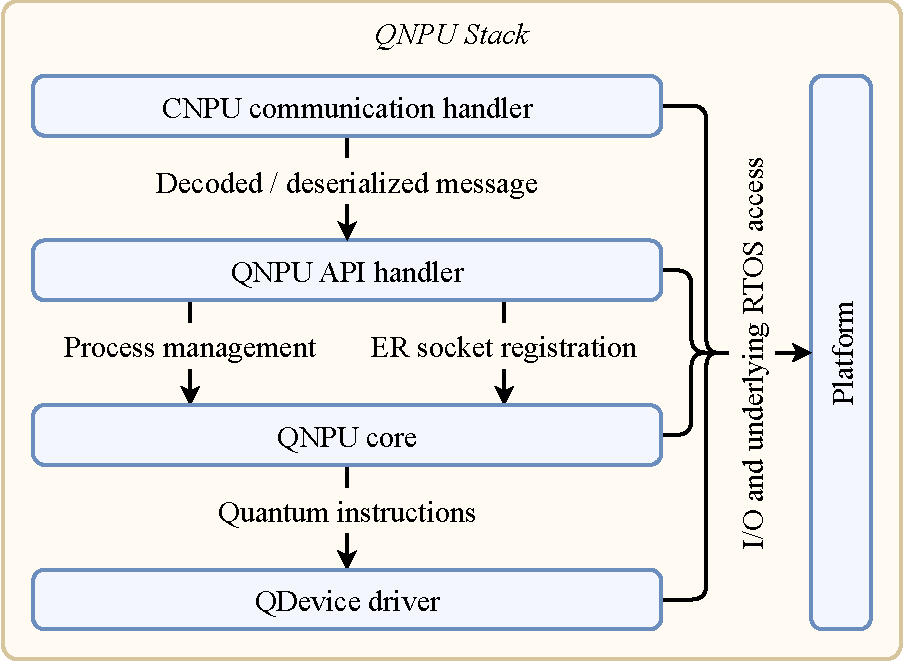
\includegraphics[width=0.6\textwidth]{figures/qnodeos/supplementary/qnodeos-stack.pdf}
\end{center}
\caption[]{\ac{QNPU} stack. The \emph{\ac{QNPU} \acs{API} handler} and \emph{the \ac{QNPU} core} form the central processing layers, and are independent of the underlying quantum physical platform and of the device where \ac{QNodeOS} runs. The \emph{\ac{CNPU} communication handler} translates protocol-specific messages from the \ac{CNPU} into \acs{API} calls. The \emph{\ac{QDevice} driver} (or \ac{QDriver}) abstracts the \ac{QDevice} hardware. The \emph{Platform} layer abstracts the hardware where \ac{QNodeOS} runs, and is accessible to all other layers. Note that three other \ac{API} types are implemented, i.e. \emph{control}, \emph{management}, and \emph{operations}. Control \ac{API} is used for the network schedule, while management and operations \ac{API} are for operational purposes. }
\label{qnodeos:fig:qnodeos-stack}
\end{figure}

\ac{QNodeOS} is a system consisting of multiple abstraction layers, as depicted in \cref{qnodeos:fig:qnodeos-stack}. It is designed to be platform-independent, i.e., independent of the underlying quantum physical platform (quantum hardware) controlled by \ac{QNodeOS}, where connections to different realizations of \ac{QDevice} are captured by a platform-dependent \ac{QDriver}. The implementation of \ac{QNodeOS} itself is of course dependent on the classical physical platform(s) on which \ac{QNodeOS} is implemented, including the physical interface between the \ac{CNPU} and \ac{QNPU}.

\subsubsection{QNPU API}
\label{qnodeos:sec:QNPU-api}

At the center of the stack lie the \emph{the \ac{QNPU} \ac{API} handler} layer and the \emph{the \ac{QNPU} core} layer. The \ac{API} handler is responsible for listening to system calls made to the the \ac{QNPU} \ac{API}, and to relay these calls to the appropriate component inside of the core layer. Such system calls may originate from the \ac{CNPU} via the \emph{CNPU communication handler}, see again~\cref{qnodeos:fig:qnodeos-stack}. 

The \ac{QNPU} \ac{API} is the central engine for managing the execution of local quantum operations and entanglement requests, and manages the hardware resources of the \ac{QDevice}. The \ac{QNPU} \ac{API} exposes services to:
%
\begin{itemize}
\item \emph{Register and deregister a program on the \ac{QNPU}}; This is part of the \ac{NetQASM} interface (see~\cref{qnodeos:sec:design:network-application}).
\item \emph{Add a quantum block (subroutine) for a user process}; This is again part of the \ac{NetQASM} interface.
\item \emph{Open an \ac{ER} socket with a remote node} (\ac{NetQASM} interface).
\item \emph{Control to configure the quantum network stack}, i.e., to configure the network schedule; This is used for the interaction with a network controller that sets network-wide entanglement schedules, as presented in Ref.~\cite{skrzypczyk_2021_arch}.
\item \emph{Perform management and operations functions.}
\end{itemize}
%
The topmost horizontal layer is the \emph{\ac{CNPU} communication handler}, which implements a \emph{protocol wrapper} around \ac{NetQASM}.
We implement this wrapper protocol using EmbeddedRPC~\cite{erpc} for the on-the-wire definition of the messages (including (de-)serialization)). The communication handler translates protocol-specific messages into \ac{API} calls for the \ac{QNPU}. EmbeddedRPC allows to decouple the interface definition and (de-)serialization from the underlying transport layer. We note that only the transport layer is implementation-specific, which depends on the devices where \ac{CNPU} and \ac{QNPU} are implemented and on what the physical interface between them looks like.\footnote{TCP/IP for now, shared memory in the future.}

The \emph{\ac{QDevice} driver} (\ac{QDriver}) layer, at the bottom of the stack, provides an abstraction of the \ac{QDevice} hardware, and its implementation depends on the nature of the \ac{QDevice} itself, and on the physical communication interface between \ac{QNPU} and \ac{QDevice}. Two \ac{QDevice} implementations may differ in a variety of factors, including what quantum physical platform they feature and what digital controller interfaces with the \ac{QNPU}.

Lastly, the vertical \emph{Platform} layer provides \ac{SoC}-specific abstractions for the \ac{QNPU} to access the physical resources of the platform it is implemented on, including I/O peripherals, interrupts controllers and timers. Additionally, if the \ac{QNPU} is implemented on top of a lower-level operating system, this layer gives access to system calls to the underlying \ac{OS}. The Platform layer is vertical to indicate that it can be accessed by all other \ac{QNPU} layers.

Porting the \ac{QNPU} to a different \ac{SoC} (or similar hardware) boils down to implementing a new platform layer. Deploying the \ac{QNPU} on a different \ac{QDevice}, instead, requires both a new \ac{QDriver} and a compiler---on the \ac{CNPU}---that emits quantum instructions supported by the specific \ac{QDevice}.

\subsection{Processes}
\label{qnodeos:sec:design:processes}

A quantum network program starts on the \ac{CNPU}---there, the \ac{CNPU} environment compiles it into classical and quantum code blocks, and creates a new process associated with the program. In the future, an optimized compilation ahead of execution could produce an executable that includes further information (such as execution deadlines depending on the device's memory lifetimes, as mentioned at the beginning of~\cref{qnodeos:sec:design:network-application}). The \ac{CNPU} then registers the program with the \ac{QNPU} (through the \ac{QNPU}'s end node \ac{API}, see \cref{qnodeos:sec:design:qnpu_stack}), which, in turn, creates its own process associated with the registered program. The process on the \ac{CNPU} is a standard \ac{OS} process, which executes the classical code blocks and interacts, (that is: communicating NetQASM subroutines and their results between \ac{CNPU} and \ac{QNPU}), with the counterpart process on the \ac{QNPU}. This interaction can be done by means of a shared memory (and when no shared memory is physically realized: by an exchange of messages~\cite{dahlberg_2022_netqasm}). On the \ac{QNPU}, a process encapsulates the execution of quantum code blocks of a program with associated context information, such as process owner, process number (ID), process state, and process priority.

In the near-term test applications we execute, the execution time of a program is typically dominated by that of quantum blocks, as entanglement generation is a time-consuming operation. Without advanced quantum repeaters~\cite{RepeaterSurvey}, its duration grows exponentially with the distance between the nodes. For this reason, we focus on the scheduling of quantum blocks only, and thus we only discuss \ac{QNPU} processes (also referred to as \emph{user processes}) from this point onward. Again, this does not exclude that in a future iteration of the design \ac{CNPU} and \ac{QNPU} could be merged into one system, and therefore classical and quantum blocks would be scheduled jointly.

\subsubsection{Process Types and Their Interaction}

\paragraph{QNPU user processes}

The \ac{QNPU} allocates a new \emph{user process} to each quantum network program registered by the \ac{CNPU}. A user process is the program's execution context, and consists of \ac{NetQASM} blocks and other context information---the process control block---including process number (ID), process owner, process state, process scheduling priority, program counter, and pointers to process data structures. Process state and priority determine how processes are scheduled on the \ac{QNPU}. A user process becomes active (ready to be scheduled) as soon as the \ac{QNPU} receives a quantum code block from the \ac{CNPU}. Multiple user processes---relative to different \ac{CNPU} programs---can be concurrently active on the \ac{QNPU}, but only one can be running at any time. A running user process executes its quantum code block directly, except for entanglement requests, which are instead submitted to the quantum network stack and executed asynchronously.

\paragraph{QNodeOS network process}

The \ac{QNPU} also defines \emph{kernel processes}, which are similar to user processes, but are created when the system starts (on boot) and have different priority values. Currently, the only existing kernel process is the \emph{network process}. The network process, owned by the \ac{QNetStack}, handles entanglement requests submitted by user processes, coordinates entanglement generation with the rest of the network, and eventually returns entangled qubits to user processes. The activation of the network process is dictated by a network-wide entanglement generation schedule. Such a schedule defines when a particular entanglement generation request can be processed, and therefore it has intersecting entries on adjacent nodes (given that entanglement is a two-party process). The schedule can be computed by a centralized network controller~\cite{skrzypczyk_2021_arch} or by a distributed protocol~\cite{dahlberg_2019_egp}. In our design, the network process follows a \emph{time division multiple access schedule}, computed by a centralized network controller (as originally proposed by \textcite{skrzypczyk_2021_arch}) and installed on each \ac{QNodeOS} node (see~\cref{qnodeos:sec:arch-networking}).

\begin{figure}
\begin{center}
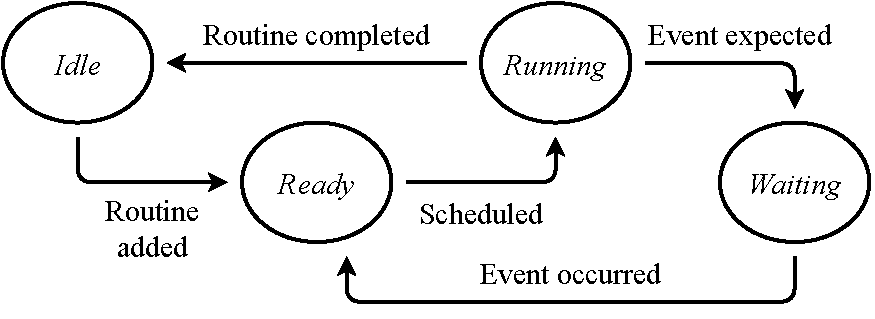
\includegraphics[width=0.6\textwidth]{figures/qnodeos/supplementary/process-states.pdf}
\end{center}
\caption[]{Process state diagram. An \emph{idle} process becomes \emph{ready} when a block for that process is loaded onto the \ac{QNPU} (from the \ac{CNPU}). A ready process becomes \emph{running} when it is scheduled. A running process goes back to idle if all blocks are completed, or transitions to \emph{waiting} if it expects an event to occur before it can proceed. A waiting process becomes ready again when the expected event occurs.}
\label{qnodeos:fig:process-states}
\end{figure}

\paragraph{QNPU process states}

A \ac{QNPU} process can be in any of the following states:
%
\begin{inlinelist}
\item \emph{Idle}: when the \ac{CNPU} has registered a program and the \ac{QNPU} has spawned a process, but it has not received a block yet;
\item \emph{Ready}: when it has (at least) one block, sent from the \ac{CNPU}, and can be scheduled and run;
\item \emph{Running}: when it is running on the \ac{QNPU} and has the quantum processor and the quantum network device assigned to it;
\item \emph{Waiting}: when it is waiting for some event to occur.
\end{inlinelist}
%
\Cref{qnodeos:fig:process-states} shows the possible process states and the valid state transitions. A process transitions from idle to ready when one block gets added. A ready process transitions to running when the the \ac{QNPU} scheduler assigns it to the processor. A running process transitions to waiting when it has to wait for an event to occur, and transitions from waiting to ready when the event occurs---for instance, a process could be waiting for an \ac{EPR} pair to be generated, and become ready again when the pair is established. Finally, a process goes back to the idle state when all its blocks have been completed.

\paragraph{Inter-process communication}

At the moment, the \ac{QNPU} does not allow for any explicit inter-process communication. The only indirect primitive available to processes to interact with one another is \emph{qubit ownership transfer}, used when a process produces a qubit state which is to be consumed by another process. Most notably, the quantum network stack kernel process transfers ownership of the entangled qubits that it produces to the process which requested the \ac{EPR} pairs.

\paragraph{Process concurrency}

The strict separation between local quantum processing and quantum networking is a key design decision in \ac{QNodeOS}, as it helps us address the scheduling challenge, see~\cref{qnodeos:sec:design-consid:challenges}. A user process can continue executing local instructions even after it has requested entanglement. Conversely, networking instructions can execute asynchronously of local quantum instructions. This is important in a quantum network, since entanglement generation must be synchronized with the neighboring node (and possibly the rest of the network~\cite{skrzypczyk_2021_arch}). Additionally, separating user programs into user processes also allows \ac{QNodeOS} to schedule several programs \emph{concurrently}.

\begin{figure}
\centering
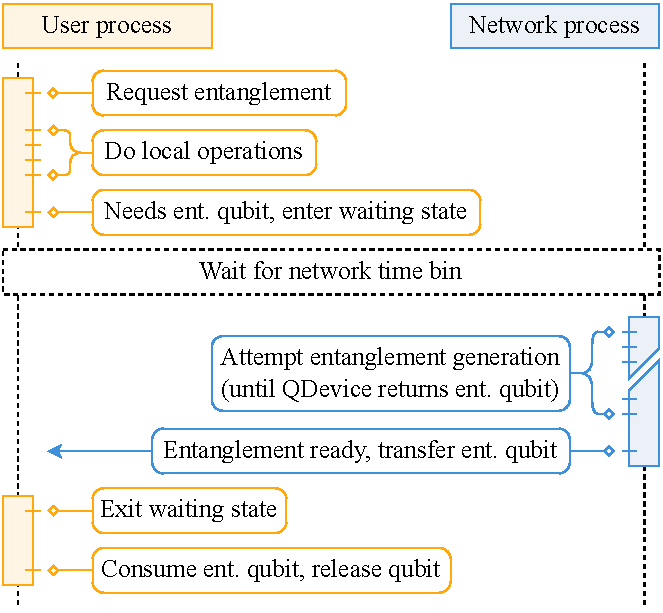
\includegraphics[width=0.6\textwidth]{figures/qnodeos/supplementary/process-flow.pdf}
\caption{Flow of execution between a user process requesting entanglement and the network process responsible for generating entanglement. The user process starts by asynchronously issuing an entanglement request. Once issued, it is free to continue with other local operations or classical processing. Once it reaches a point in its execution where entanglement is required the process enters the waiting state. The network process is scheduled once the appropriate time bin (as determined by the network schedule) starts. Once running, it attempts entanglement generation until entanglement success (or until a set timeout). The entangled qubit is then transferred to the user process. This unblocks the process which consumes the entanglement and releases the qubit. In our experiments, the process always immediately waits after requesting entanglement (no local operations are done in between).}
\label{qnodeos:fig:process-flow}
\end{figure}

\paragraph{Process flow}

\cref{qnodeos:fig:process-flow} illustrates the typical control flow between a user process and the network process. User processes are free to execute any non-networked instructions independently of the network process and other user processes. Once the program reaches a point in its execution where an entangled qubit is required, the process enters the waiting state and is flagged as waiting for entanglement. When the network process is scheduled, it issues network instructions and generates entanglement as requested by the user process. Once an entangled pair is generated by the network process, the qubit is handed over to the waiting user process. When all the entangled pairs that the user process was waiting for are delivered, the user process becomes ready and can start running again.

\subsubsection{Process Scheduling}
\label{qnodeos:sec:design:scheduling}

At present, the the \ac{QNPU} scheduler does not give any guarantees on when a process is scheduled---for that, one would need to define concrete real-time constraints to feed to the scheduler. Instead, the current version of the \ac{QNPU} implements a best-effort scheduler, which selects processes on the basis of their \emph{priority}, and does not allow preemption. In particular, the network process is assigned the highest priority, and is activated whenever the network schedule specifies entanglement should be made in the next time-bin~\cite{skrzypczyk_2021_arch}. 

As already mentioned, \ac{QNodeOS} defines the concept of \emph{user} processes and \emph{kernel} processes, with the \ac{QNetStack} process being the only kernel process at the moment. User processes are released (i.e., they become ready) asynchronously---when a process block is loaded, or when they leave the waiting state---while the \ac{QNetStack} process is released periodically---at the beginning of each time bin of the network schedule (although the period of time bins can vary). Given that generating an \ac{EPR} pair on a link requires that both nodes attempt entanglement simultaneously, the \ac{QNPU} assigns the \ac{QNetStack} process a priority higher than any user process. This ensures that, at the beginning of each time bin of the network schedule, the \emph{priority-based} process scheduler can assign the \ac{QNetStack} process as soon as the processor is available, and thus a node can start attempting entanglement with its neighbor as soon as possible and minimize wasted attempts on the neighbor node.

\Cref{qnodeos:fig:scheduling-impl} exemplifies a snapshot of a hypothetical execution of a user process and the \ac{QNetStack} process. The latter is activated at the beginning of a time-bin assigned to networking, and is scheduled as soon as the processor is available---for instance, at times $0$ and $4$ it is scheduled immediately, while at time $8$ it is scheduled after one time unit, as soon as the running process yields. The user process becomes ready at time $0$---at which point the \ac{QNetStack} process is ready as well and has highest priority, meaning the network process is scheduled; then it is scheduled at time $2$, as soon as the \ac{QNetStack} process completes; then it goes into waiting state at time $3$ because the user process requested entanglement and it waits for the entanglement to be established; finally it becomes ready again at time $7$---and it is scheduled immediately given that no other processes are running.

\begin{figure}
\begin{center}
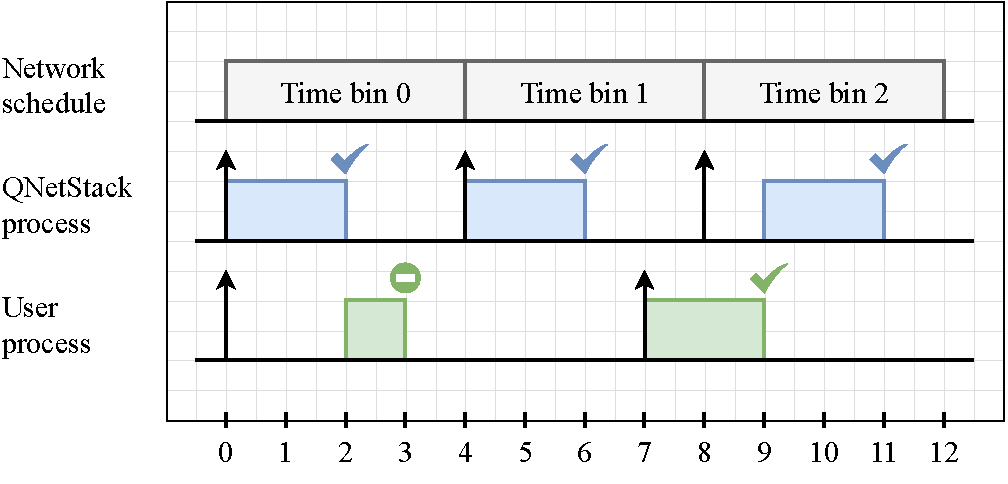
\includegraphics[width=0.7\textwidth]{figures/qnodeos/supplementary/scheduling-impl.pdf}
\end{center}
\caption[]{Snapshot of a hypothetical execution of a user process and the \ac{QNetStack} process. The higher-priority \ac{QNetStack} process is activated at the start of each time bin of the network schedule, and it is assigned to the processor as soon as it is available. The lower-priority user process gives precedence to the \ac{QNetStack} process when they become ready at the same time, but, when it is running on the processor, it is not preempted if the \ac{QNetStack} process becomes ready while the user process is running. Black arrows represents a moment where the process goes into the ready state and the green stop sign (at time $3$) represents a process going into the waiting state.}
\label{qnodeos:fig:scheduling-impl}
\end{figure}

To avoid context switching overhead, potentially leading to degraded fidelity, the \ac{QNPU} scheduler is \emph{cooperative}. That is, once a process is scheduled, it gets to run until it either completes all of its instructions or it blocks waiting for entanglement. Allowing process preemption would need a definition of critical section and could potentially impact the quality of the affected qubit states. Moreover, the lack of a preemption mechanism could potentially result in low-priority user processes hogging the processor at the expense of high-priority entanglement generation attempts. On the other hand, if entanglement instructions always consume the entirety of the time bin, the \ac{QNetStack} process would be immediately assigned the processor each time it relinquishes it, causing low-priority user processes to starve. To at least mitigate the second issue, we made sure that the number of consecutive entanglement attempts performed by the \ac{QDevice} within one single entanglement instruction is always less than how many would fit in a time bin, so as to leave some slack for low-priority user processes to run.

\subsubsection{Networking}
\label{qnodeos:sec:arch-networking}

The network stack \ac{QNetStack} is based on the existing stack~\cite{dahlberg_2019_egp}, including the link layer \ac{QEGP}~\cite{dahlberg_2019_egp}.
However the main difference between the \ac{QNetStack} implemented on the \ac{QNPU} and the original design of the protocols lies in how the \ac{QEGP} processes the outstanding entanglement requests. \ac{QEGP}~\cite{dahlberg_2019_egp} employed the concept of a distributed queue to sort and schedule entanglement requests on one node by coordinating with the counterpart node on the other end of the link, to ensure that both nodes would be servicing the same entanglement request at any given time. This synchronization is necessary because different entanglement requests may require different \ac{EPR} pair fidelities, in which case \ac{QEGP} would issue different \ac{QDevice} entanglement instructions. However, link-local request scheduling becomes more complicated if nodes have more than just one link. In that case, entanglement requests would be better scheduled at a level where network-wide request schedules are known. 

\paragraph{Network Schedule}
The \ac{QEGP} protocol implemented on the \ac{QNPU} transitioned~\cite{pompili_2022_experimental} from scheduling entanglement requests via a pairwise agreed upon distributed queue, to deferring this task to a \emph{logically centralized control plane}, whereby a node's schedule can be computed on the basis of the whole network's needs by a (logically) centralized controller (see e.g.~\cite{skrzypczyk_2021_arch}). This means that the network stack of the nodes convey their demands for end-to-end entanglement generation to the central controller, who then makes a \emph{network schedule}, which is communicated back to the nodes. 

All nodes divide time into time-bins, where the central controller employs a scheduling algorithm to assign either network actions (or no actions) to time-bins. That is, the term network schedule refers to a schedule, i.e. allocation of resources over time, of time-bins at the nodes, where a time-bin may be marked for networking activities (entanglement generation) or be left empty (to be used arbitrarily to execute local operations). 
Given that entanglement generation requires a non-deterministic amount of attempts and time, time bins are computed to be large enough to accommodate the average run time of an entanglement generation instruction. 
We remark that the node functions internally as a higher timing granularity than a time-bin allocated by the network scheduler, that is, it can execute other operations (such as for example local quantum operations) also within a time-bin allocated by the network schedule, provided entanglement is made early.

Once the node received the network schedule from the controller, the network schedule is used to satisfy all outstanding end-to-end entanglement requests, and is used by \ac{QEGP} to produce the correct \ac{QDevice} instructions at any point in time. Whenever a time bin is assigned to networking to two neighboring nodes, the nodes attempt entanglement generation over their shared link in order to realize the \ac{QEGP} link layer protocol. 
\Cref{qnodeos:fig:qnetstack-impl} shows internal components and data structures of the \ac{QNetStack} as it is implemented on the \ac{QNPU}. Entanglement requests received by the \ac{EMU} are forwarded by \ac{QNP} to the next hop's \ac{QNPU} system. Entanglement requests and network schedule---the latter installed by a logically centralized control plane---are used by \ac{QEGP} to produce the correct entanglement instructions to populate the \ac{QNetStack} process's block at each activation of the process.

\begin{figure}
\begin{center}
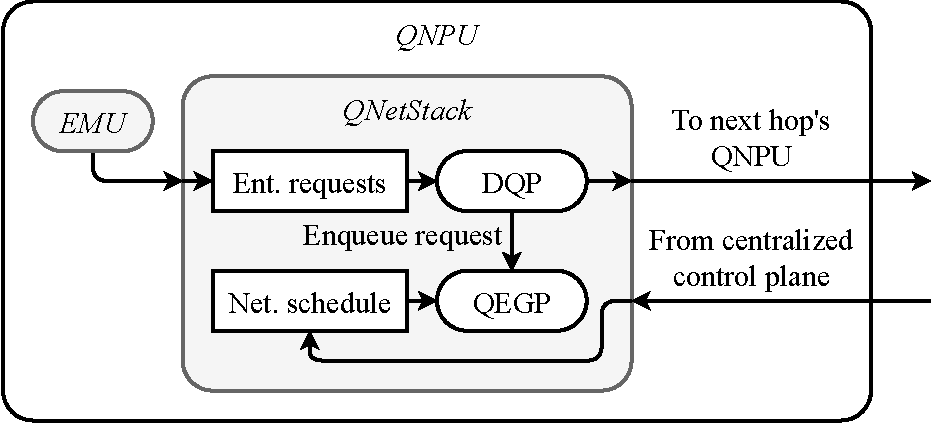
\includegraphics[width=0.6\textwidth]{figures/qnodeos/supplementary/qnetstack-impl.pdf}
\end{center}
\caption[]{Internal components and data structures of the \acf{QNetStack}. Entanglement requests are received through the \acf{EMU}, while the network schedule is installed by a centralized control plane. 
\acf{QEGP} maps such requests onto the network schedule to produce the correct entanglement instructions. While not needed on our 2 node implementation, a \ac{DQP} (which is a simplified version of the \ac{DQP} presented in~\cite[Section 5.2.1]{dahlberg_2019_egp}) could forward entanglement requests to the next hop's \acf{QNPU} to realize a network layer protocol such as~\cite{kozlowski_2020_qnp}.}.
\label{qnodeos:fig:qnetstack-impl}
\end{figure}

\paragraph{ER Socket}
\label{qnodeos:sec:design_er_socket}
The concept of an \ac{ER} socket is inspired by that of a classical network socket, in that it defines the endpoint of an entanglement generation request, and is used by the \ac{QNPU}'s quantum network stack to set up network tables and to establish connections with its peers. 
We remark that the current realization of the \ac{ER} Socket (see below) is a proof of concept implementation opening future computer science research, and does not aim to prevent misuse if different users had access to the same node. 
A program can request from QNodeOS the opening of an \ac{ER} socket with a program on a remote node. An \ac{ER} socket is identified by the tuple \texttt{(node\_id, er\_socket\_id, remote\_node\_id, remote\_er\_socket\_id)}. The other program (on the other node) must open its own corresponding \ac{ER} socket (i.e with values \texttt{(remote\_node\_id, remote\_er\_socket\_id, node\_id, er\_socket\_id)}) on its own QNodeOS. A request for opening an \ac{ER} socket is executed by the CNPU, by asking the QNPU (through the QNPU API) to open the socket. The QNPU then registers the ER socket with the quantum network stack (provided it did not yet exist), and the CNPU also keeps a reference using the tuple as an identifier. The program can then use this socket for requests. The network stack only handles requests for entanglement between two nodes if the corresponding \ac{ER} sockets are opened on both nodes.

Programs are themselves responsible for coordinating the ER socket IDs. Using these IDs allow the same node pair to open multiple pairs of ER sockets, which may be used by different applications or inside the same application. Socket IDs must be unique within the node. \ac{ER} sockets are typically opened at the start of a program, and live (and may be used multiple times) until the program finishes.

Programs use the \ac{ER} socket to submit entanglement requests to the network stack. This is done through NetQASM instructions (\texttt{create\_epr} and \texttt{recv\_epr}) that refer to the \ac{ER} socket in their operands. One program must execute a \texttt{create\_epr} instruction and the other a \texttt{recv\_epr} instruction (to be coordinated by the programs themselves). The program executing the \texttt{create\_epr} instruction is treated by the network stack as the \emph{initiator} and the program executing \texttt{recv\_epr} the \emph{receiver}. 
Upon receiving an entanglement request, the network stacks of the two nodes communicate between each other in order to coordinate entanglement generation. The initiator node always initiates this communication. The receiver node always accepts the entanglement initiative as long as the corresponding \ac{ER} socket is open. This means that the receiver node agrees with entanglement generation as soon as the initiator node has submitted an entanglement request (through its \texttt{create\_epr}), even if the receiver node itself has not yet submitted its corresponding request (through its \texttt{recv\_epr}). On the receiver node, the generated entangled qubit will remain in memory until it gets asked for by a user process executing this \texttt{recv\_epr}.

\subsubsection{Multitasking}

Multi-tasking forms an essential element of our architecture already at the level of scheduling the network process in relation to any user process, to address the challenges inherent in the way entanglement is produced at the physical layer, requiring agreement on a network schedule (see \cref{qnodeos:sec:arch-networking}). For this important reason, the \ac{QNPU} is designed to arbitrate between these two processes (see \cref{qnodeos:fig:process-flow}), and to manage the resources being used by each of them. \emph{Multitasking}, hence, is a fundamental requirement for a system managing the hardware of a quantum network node, especially while such hardware has only limited resources available. 

To further increase the utility of the system, we also allow the multi-tasking of user processes.
Like in most operating systems, these tasks, which on the \ac{QNPU} are encapsulated into processes, can sometimes necessitate a resource which is not immediately available---for instance, a free qubit, or a qubit entangled with a remote one. Maximizing the utilization of the quantum device is also one of the goals of \ac{QNodeOS}, whose design allows multiple processes, user and kernel, to be active concurrently, so that whenever one is in a waiting state, another one can potentially be scheduled to use the quantum device.  This design aspect is relevant for quantum networking nodes, as the execution of the local program is often waiting, both for classical messages from remote nodes, as well as the generation of entanglement. 

Lastly, multitasking is an important feature for systems that are to be shared by multiple users, and that offer each user the possibility to run multiple programs concurrently. The multitasking capabilities of \ac{QNodeOS} are also aimed at improving the average throughput and latency of user programs.


\subsection{QNodeOS components and interfaces}
\label{qnodeos:sec:appendix-qnodeos-core}

\begin{figure*}
\begin{center}
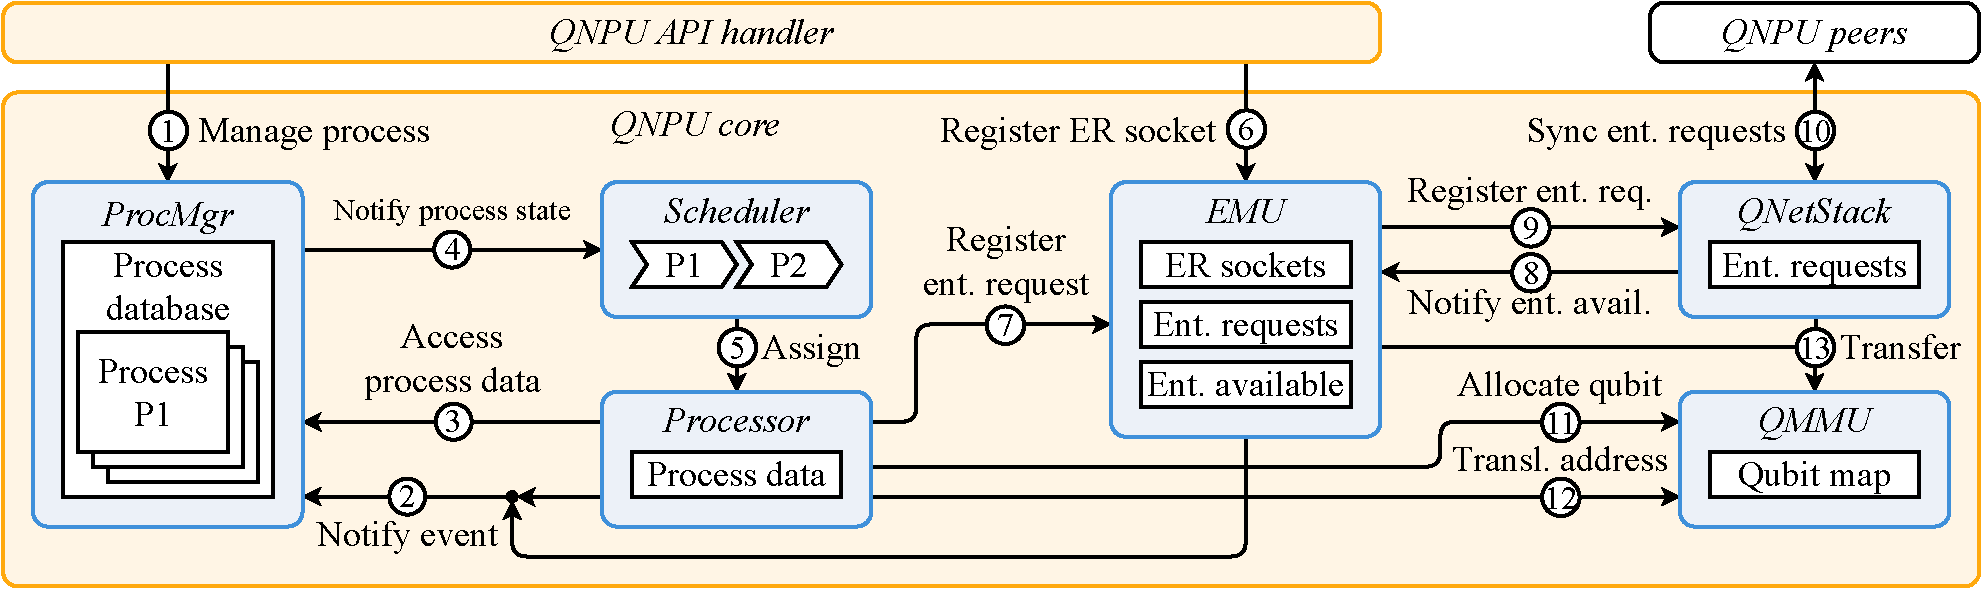
\includegraphics[width=1.0\textwidth]{figures/qnodeos/supplementary/qnodeos-core.pdf}
\end{center}
\caption[]{\acf{QNPU} core components and internal interfaces. The core layer includes:
\begin{inlinelist}
\item a \emph{process manager} (ProcMgr), which owns and manages access to \ac{QNPU} processes;
\item a \emph{scheduler}, responsible for selecting the next process to be run;
\item a \emph{processor}, which processes blocks' instructions;
\item an \emph{\ac{EMU}}, which keeps a list of entanglement requests and available entangled qubits;
\item a \emph{\ac{QNetStack}}, whose responsibility is to coordinate with peer nodes to schedule quantum networking instructions;
\item a \emph{\ac{QMMU}}, which keeps a record of allocated qubits.
\end{inlinelist}
}
\label{qnodeos:fig:qnodeos-core}
\end{figure*}

We provide here additional details on the components of the \ac{QNPU} architecture and their interfaces. \Cref{qnodeos:fig:qnodeos-core} gives an overview of all the components of the \ac{QNPU}. The \emph{process manager} marshals accesses to all user and kernel processes. The \emph{scheduler} assigns ready processes to the \emph{processor}, which runs quantum instructions through the underlying \ac{QDevice}, processes classical \ac{NetQASM} instructions locally, and registers entanglement requests with the \emph{\ac{EMU}}. The \ac{EMU} maintains a list of \ac{ER} sockets and entanglement requests, forwards the latter to the \emph{quantum network stack}, which, in turn, registers available entangled qubits with the \ac{EMU}. Finally, the \emph{\ac{QMMU}} keeps track of used qubits, and transfers qubit ownership across processes when requested.

\subsubsection{Process Manager}

The process manager owns \ac{QNPU} processes and marshals accesses to those. Creating a process, adding a block to it and accessing the process's data must be done through the process manager. Additionally, the process manager is used by other components to notify \emph{events} that occur inside the \ac{QNPU}, upon which the state of one of more processes is updated. Process state updates result in a notification to the scheduler.

\paragraph{Interfaces}

The process manager exposes interfaces for three services:
%
\begin{itemize}
\item Process management (interface 1 in \cref{qnodeos:fig:qnodeos-core}): to create and remove processes, and to add quantum blocks to them. When the user registers a program, the the \ac{QNPU} \ac{API} Handler uses the process manager to create a \ac{QNPU} user process. The returned process ID can be later used to add a block to that process, or to remove the process once all its blocks are fully processed.
\item Event notification (interface 2 in \cref{qnodeos:fig:qnodeos-core}): to notify an event occurred inside the \ac{QNPU}, including the addition of a block, the completion of a block, the scheduling of the process, the hitting of a \emph{Waiting} condition (see \cref{qnodeos:fig:process-states}), and the generation of an entangled qubit destined to the process. Some events trigger follow-up actions---for instance, when a process that was waiting for an event becomes ready, it gets added to the queue of ready processes maintained by the scheduler.
\item Process data access (interface 3 in \cref{qnodeos:fig:qnodeos-core}): to access a process's blocks and its classical memory space, mostly used while running the process (through the processor).
\end{itemize}

\subsubsection{Scheduler}

The \ac{QNPU} scheduler registers processes that are ready to be scheduled, and assigns them to the \ac{QNPU} processor when the latter is available. Ready processes are stored in a \emph{prioritized ready queue}, and processes of the same priority are scheduled with a first-come-first-served policy.

\paragraph{Interfaces}

The scheduler only exposes one interface for process state notifications (interface 4 in \cref{qnodeos:fig:qnodeos-core}), used by the process manager to signal when a process transitions to a new state. When a \ac{QNPU} process transitions to the ready state, it is directly added to the scheduler's prioritized ready queue. When a process becomes idle, or is waiting for an event to happen, the scheduler simply registers that the processor has become available.

\subsubsection{Processor}

The \ac{QNPU} processor handles the execution of \ac{QNPU} user and kernel processes, by running classical instructions locally and issuing quantum instructions to the \ac{QDriver}. It is also responsible for multitasking by means of process manager. While executing a process, the processor reads its blocks and accesses (reads and writes) its classical memory. The processor implements a specific instruction set architecture dictated by the \ac{NetQASM} language of choice.

\paragraph{Interfaces}

The processor exposes one interface for processor assignment (interface 5 in \cref{qnodeos:fig:qnodeos-core}), used by the \ac{QNPU} scheduler to activate the processor, when it is idling, and assign it to a \ac{QNPU} process.

\subsubsection{Entanglement Management Unit}

The \acf{EMU} contains a list of open \emph{\ac{ER} sockets} and a list of \emph{entanglement requests}, and keeps track of the \emph{available entangled qubits} produced by the quantum network stack. Received entanglement requests are considered valid only if an \ac{ER} socket associated to such requests exists. Valid requests are forwarded to the quantum network stack. Entangled qubit generations are notified as events to the process manager.

\paragraph{Interfaces}

The \ac{EMU} exposes interfaces for three services:
%
\begin{itemize}
\item \ac{ER} socket registration (interface 6 in \cref{qnodeos:fig:qnodeos-core}): to register and open \ac{ER} sockets belonging to a program, and to set up internal classical network tables and to establish classical network connection.
\item \ac{ER} registration (interface 7 in \cref{qnodeos:fig:qnodeos-core}): to add entanglement requests to the list of existing ones, to be used when matching produced entangled qubits with a process that requested them.
\item Entanglement notification (interface 8 in \cref{qnodeos:fig:qnodeos-core}): to register the availability of an entangled qubit, produced by the quantum network stack, and to link it to an existing entanglement request.
\end{itemize}

\subsubsection{Quantum Network Stack}

The quantum network stack on the \ac{QNPU} closely follows the model presented by
\textcite{dahlberg_2019_egp} which is based on the classical \ac{OSI} network stack model for the purpose of the separation of responsibilities. In particular, \emph{data link layer} is part of the quantum network stack on the \ac{QNPU}. The \emph{physical layer} is implemented on the \ac{QDevice}, the \emph{application layer} is part of the \ac{CNPU}, and all remaining layers are not currently part of the stack.

The quantum network stack component has an associated \emph{\ac{QNPU} kernel process}, created statically on the \ac{QNPU}. However, this process's block is dynamic: the instructions to be executed on the processor depend on the outstanding entanglement generation requests received from \ac{EMU} and network peers.

\paragraph{Interfaces}

The quantum network stack exposes interfaces for two services:
%
\begin{itemize}
\item Entanglement request registration (interface 9 in \cref{qnodeos:fig:qnodeos-core}): to add entanglement requests coming from the \ac{EMU} to the list of existing ones, which are used to fill in the quantum network stack process's block with the correct quantum instructions to execute.
\item Entanglement request synchronization (interface 10 in \cref{qnodeos:fig:qnodeos-core}): similar to the entanglement request registration interface, but to be used to synchronize (send and receive) requests with \ac{QNodeOS} network peers.
\end{itemize}

\subsubsection{Quantum Memory Management Unit}

\acf{QMMU} receives requests for \emph{qubit allocations} from \ac{QNPU} processes, and manages the subsequent usage of those. It also translates \ac{NetQASM} \emph{virtual qubit addresses} into physical addresses for the \ac{QDevice}, and keeps track of which process is using which qubit at a given time. In general, a \ac{QMMU} should take into account that the topology of a quantum memory determines what operations can be performed on which qubits, and thus allow processes to allocate qubits of a specific type upon request. An advanced \ac{QMMU} could also feature algorithms to move qubits in the background---that is, without an explicit instruction from a process's block---to accommodate a program's topology requirements while not trashing the qubits being used by other \ac{QNPU} processes. Such a feature could prove crucial to increase the number of processes that can be using the quantum memory at the same time, and to enhance multitasking performances.

\paragraph{Interfaces}

The \ac{QMMU} exposes interfaces for three services:
%
\begin{itemize}
\item Qubit allocation and de-allocation (interface 11 in \cref{qnodeos:fig:qnodeos-core}): a running process can ask for one or more qubits, which, if available, are allocated by the \ac{QMMU}, and the physical addresses of those are mapped to the virtual addresses provided by the requesting process.
\item Virtual address translation (interface 12 in \cref{qnodeos:fig:qnodeos-core}): before sending quantum instructions to the \ac{QDriver}, the processor uses virtual qubit addresses specified in \ac{NetQASM} to retrieve physical addresses from the \ac{QMMU}, and then replaces virtual addresses with physical addresses in the instructions for the \ac{QDriver}.
\item Qubit ownership transfer (interface 13 in \cref{qnodeos:fig:qnodeos-core}): qubits are only visible to the process that allocates them. However, in some cases, a process may wish to transfer some if its qubits to another one. A notable example is the quantum network process transferring an entangled qubit to the process that will use it.
\end{itemize}

\subsection{QNPU implementation: scheduler}
\label{qnodeos:sec:qnpu_impl_scheduler}
The \ac{QNPU} scheduler is an important component of our \ac{QNodeOS} architecture, and deals with scheduling of QNPU processes. The QNPU is implemented on FreeRTOS~\cite{freertos}, which itself includes a scheduler. On FreeRTOS, code is organized into tasks, which can be seen as separate threads or processes. These tasks are scheduled concurrently by FreeRTOS based on priority. In our implementation, we realize QNPU components and interfaces (hence including the QNPU scheduler) as FreeRTOS tasks. We configured task priorities such that the components with tight interaction with the QDevice (\ac{QDriver}, quantum network stack, QNPU processor) have highest priority.
We stress the difference between the FreeRTOS scheduler and our QNPU process scheduler. 
The QNPU scheduler schedules QNPU processes based on their status and priorities, which are independent of the priorities assigned by the FreeRTOS scheduler.
The FreeRTOS hence runs on a different layer: it makes sure the QNPU components (including QNPU scheduler, processor, \ac{QDriver}) run concurrently. The QNPU scheduler runs on the level of QNPU processes. Whenever the FreeRTOS scheduler activates the FreeRTOS task realizing the QNPU scheduler, the QNPU scheduler then schedules the process with the highest priority on a first come first serve basis, by adding it to the processing queue of the relevant resource (e.g. QNPU processor) and generating an interrupt leading to the execution of the QNPU processor task on FreeRTOS (and consequently the execution of the process).

\subsection{QDevice interface}
\label{qnodeos:sec:appendix-qdevice}

The implementation of a \ac{QDevice} depends on a number of factors. Most importantly, the physical signals that are fed to the quantum processing and networking device (and those that are output from the device) are specific to the nature of the device itself. Different qubit realizations require different digital and analog control. For instance, manipulating the state of a spin-based qubit (e.g., in a \ac{NV} center processor) and that of an atom qubit (e.g., in a trapped ion processor) are two physical processes that vastly differ in a number of complex ways.

For \ac{QNodeOS} to be portable to a diverse set of quantum physical platforms, there needs to be a common \emph{\ac{QDevice} interface} that \ac{QNodeOS} can rely on, and that each \ac{QDevice} instance can implement as it is most convenient for the underlying quantum device. This interface \begin{inlinelist} \item needs to be \emph{general}, \item to be able to \emph{express all quantum operations} that different quantum devices might be capable of performing, and \item \emph{abstract}, so that two different implementations of a well-defined qubit manipulation operation can be expressed with the same instruction on \ac{QNodeOS}.\end{inlinelist} Nevertheless, an interface that is too general could result in a high implementation complexity on the \ac{QDevice}, as it might have to transform high-level instructions in a series of native operations on the fly. Other than complexity of implementation, a very high-level set of \ac{QDevice} instructions might compromise the compiler's ability to optimize a program for a certain physical platform, as reported by~\textcite{murali_2019_fullstack}.

\subsubsection{Design Choices}

Defining a set of instructions to express abstract quantum operations as close as possible to what different quantum physical platforms can natively perform is---to some extent---an open problem. Nonetheless, we have made an effort to specify an interface which is a good compromise between generality and expressiveness. The \ac{QDevice} interface is essentially a set of instructions that \ac{QNodeOS} expects a \ac{QDevice} to implement. To be precise, a \ac{QDevice} might implement a subset of the interface, according to what native physical operations it can perform. The CNPU compiler must then have knowledge about the set of instructions implemented by the underlying \ac{QDevice}, so that it can decompose instructions that are not natively supported.

Even though this interface does not impose any formal timing constraints, it is important to note that a \ac{QDevice} implementation that tries to guarantee more or less deterministic instruction processing latencies can prove more beneficial to the real-time requirements of the \ac{QNPU}. Particularly, it would be advisable to time-bound the processing time of operations whose duration is by nature probabilistic---most notably, those involving entanglement generation. Creating an \ac{EPR} pair may involve a varying number of attempts. Sometimes, if the remote node becomes unresponsive for some time, the number of necessary attempts can increase by a large amount. Capping the number of attempts could, for instance, provide a more deterministic maximum processing latency for entanglement instructions, which in turn might help \ac{QNodeOS} react more timely to temporary failures or downtime periods of remote nodes. Not to mention that unbounded entanglement attempts affect the state of other qubits in memory, because of both passive decoherence and cross-qubit noise.

\subsubsection{QDevice synchronization}
\label{qnodeos:sec:qdevice-sync}
The QDevice receives physical instructions from QNodeOS, acts on them, and returns a response. For entanglement instructions, the QDevice must first synchronize with the QDevice on the other node (using classical communication). If the other QDevice is busy, (e.g. it is still trying to pass the CR check, see~\cref{qnodeos:sec:qdevice-nv} and \cite{pompili_2022_experimental}), synchronization fails, and an \texttt{ENT\_SYNC\_FAIL} response is returned (see~\cref{tab:qdevice-return-values}).

\subsubsection{Instructions and Operands}
\label{qnodeos:sec:appendix-qdevice-instructions-operands}

\begin{table}[t]
\begin{tabularx}{\linewidth}{>{\ttfamily}l X}
\toprule
\normalfont{Instruction} & Description \\
\midrule
INI & Initialize a qubit to default state \\
SQG & Perform a single-qubit gate \\
TQG & Perform a two-qubit gate \\
AQG & Perform a gate on all qubits \\
MSR & Measure a qubit in a specified basis \\
ENT & Attempt entanglement generation \\
ENM & Attempt entanglement and measure qubit \\
MOV & Move qubit state to another qubit \\
SWP & Swap the state of two qubits \\
ESW & Swap qubits belonging to two \ac{EPR} pairs \\
PMG & Set pre-measurement gates \\
\bottomrule
\end{tabularx}
\caption[]{Summary of \ac{QDevice} instructions defined in the \ac{QDevice} interface. A specific \ac{QDevice} might implement a subset of these, depending on the underlying quantum physical device and on other design constraints.}
\label{tab:qdevice-instructions}
\end{table}

\Cref{tab:qdevice-instructions} lists the complete set of instructions defined in the \ac{QDevice} interface. Instructions can have operands, whose range of valid values depends on the underlying \ac{QDevice}. For instance, an operand that specifies which qubit to apply an operation to can only have as many valid values as there are physical qubits in memory. Details for each instruction and its operands are given below.

\paragraph{Qubit Initialization (\texttt{INI})}

The \texttt{INI} instruction brings a qubit to the $\ket{0}$ state. On some physical platforms, single-qubit initialization is not possible, thus this instruction initializes all qubits to the $\ket{0}$ state.

\medskip \noindent
\begin{tabularx}{\linewidth}{>{\ttfamily}l X}
\toprule
\normalfont{Operand} & Description \\
\midrule
qubit & Physical address of the qubit to initialize, ignored on platforms where single-qubit initialization is not possible \\
\bottomrule
\end{tabularx}

\paragraph{Single-Qubit Gate (\texttt{SQG})}

The \texttt{SQG} instruction manipulates the state of one qubit. The gate is expressed as a rotation in the Bloch sphere.

\medskip \noindent
\begin{tabularx}{\linewidth}{>{\ttfamily}l X}
\toprule
\normalfont{Operand} & Description \\
\midrule
qubit & Physical address of the qubit to manipulate \\
axis  & Rotation axis, can be X, Y, Z or H (support is \ac{QDevice}-dependent) \\
angle & Rotation angle (granularity and range are \ac{QDevice}-dependent) \\
\bottomrule
\end{tabularx}

\paragraph{Two-Qubit Gate (\texttt{TQG})}

The \texttt{TQG} instruction manipulates the state of two qubits. The gate is expressed as a controlled rotation, with one qubit being the control and the other one being the target.

\medskip \noindent
\begin{tabularx}{\linewidth}{>{\ttfamily}l X}
\toprule
\normalfont{Operand} & Description \\
\midrule
qub\_c & Physical address of the control qubit \\
qub\_t & Physical address of the target qubit \\
axis   & Rotation axis, can be X, Y, Z or H (support is \ac{QDevice}-dependent) \\
angle  & Rotation angle (granularity and range are \ac{QDevice}-dependent) \\
\bottomrule
\end{tabularx}

\paragraph{All-Qubit Gate (\texttt{AQG})}

The \texttt{AQG} instruction manipulates the state of all available qubits. The gate is expressed as a rotation in the Bloch sphere.

\medskip \noindent
\begin{tabularx}{\linewidth}{>{\ttfamily}l X}
\toprule
\normalfont{Operand} & Description \\
\midrule
axis  & Rotation axis, can be X, Y, Z or H (support is \ac{QDevice}-dependent) \\
angle & Rotation angle (granularity and range are \ac{QDevice}-dependent) \\
\bottomrule
\end{tabularx}

\paragraph{Qubit Measurement (\texttt{MSR})}

The \texttt{MSR} instruction measures the state of one qubit in a specified basis. A qubit measurement is destructive---that is---the qubit has to be reinitialized before it can be used again.

\medskip \noindent
\begin{tabularx}{\linewidth}{>{\ttfamily}l X}
\toprule
\normalfont{Operand} & Description \\
\midrule
qubit & Physical address of the qubit to measure \\
basis & Measurement basis, can be X, Y, Z, H (support is \ac{QDevice}-dependent) \\
\bottomrule
\end{tabularx}

\paragraph{Entanglement Generation (\texttt{ENT})}

The \texttt{ENT} instruction performs a series of entanglement generation attempts, until one succeeds, or until a maximum number of attempts is reached (the behavior is \ac{QDevice}-dependent).

\medskip \noindent
\begin{tabularx}{\linewidth}{>{\ttfamily}l X}
\toprule
\normalfont{Operand} & Description \\
\midrule
nghbr & Neighboring node to attempt entanglement with, if the local \ac{QDevice} has multiple quantum links \\
fid & Target entanglement fidelity (granularity and range are \ac{QDevice}-dependent) \\
\bottomrule
\end{tabularx}

\paragraph{Entanglement Generation With Qubit Measurement (\texttt{ENM})}

The \texttt{ENM} instruction performs a series of entanglement generation attempts followed by an immediate measurement of the local qubit, until one succeeds, or until a maximum number of attempts is reached (the behavior is \ac{QDevice}-dependent).

\medskip \noindent
\begin{tabularx}{\linewidth}{>{\ttfamily}l X}
\toprule
\normalfont{Operand} & Description \\
\midrule
nghbr & Neighboring node to attempt entanglement with, if the local \ac{QDevice} has multiple quantum links \\
fid & Target entanglement fidelity (granularity and range are \ac{QDevice}-dependent) \\ basis & Measurement basis, can be X, Y, Z, H (support is \ac{QDevice}-dependent) \\
\bottomrule
\end{tabularx}

\paragraph{Qubit Move (\texttt{MOV})}

The \texttt{MOV} instruction moves the state of one qubit to another qubit. A qubit move renders the state of the source qubit undefined, and the qubit has to be reinitialized before it can be used again.

\medskip \noindent
\begin{tabularx}{\linewidth}{>{\ttfamily}l X}
\toprule
\normalfont{Operand} & Description \\
\midrule
qub\_s & Physical address of the source qubit \\
qub\_d & Physical address of the destination qubit \\
\bottomrule
\end{tabularx}

\paragraph{Qubit Swap (\texttt{SWP})}

The \texttt{SWP} instruction swaps the state of two qubits.

\medskip \noindent
\begin{tabularx}{\linewidth}{>{\ttfamily}l X}
\toprule
\normalfont{Operand} & Description \\
\midrule
qub\_1 & Physical address of the first qubit \\
qub\_2 & Physical address of the second qubit \\
\bottomrule
\end{tabularx}

\paragraph{Entanglement Swap (\texttt{ESW})}

The \texttt{ESW} instruction results in two qubits belonging to two \ac{EPR} pairs to have their roles swapped.

\medskip \noindent
\begin{tabularx}{\linewidth}{>{\ttfamily}l X}
\toprule
\normalfont{Operand} & Description \\
\midrule
qub\_1 & Physical address of the first qubit \\
qub\_2 & Physical address of the second qubit \\
\bottomrule
\end{tabularx}

\paragraph{Pre-Measurement Gates Setting (\texttt{PMG})}

The \texttt{PMG} instruction allows for a set of (up to) 3 rotations to be performed before a qubit measurement (\texttt{MSR} or \texttt{ENM}). If the axis of the second rotation is orthogonal to the axis of the first and the third rotation, these gates can be used to perform a qubit measurement in an arbitrary basis, given that most likely a \ac{QDevice} can natively measure in a limited set of bases.

\medskip \noindent
\begin{tabularx}{\linewidth}{>{\ttfamily}l X}
\toprule
\normalfont{Operand} & Description \\
\midrule
axes & Combination of orthogonal axes to use for the three successive rotations, can be X--Y--X, Y--Z--Y and Z--X--Z (support is \ac{QDevice}-dependent) \\
ang\_1 & Rotation angle of the first gate, relative to the first axis in \texttt{axes} (granularity and range are \ac{QDevice}-dependent) \\
ang\_2 & Rotation angle of the second gate, relative to the second axis in \texttt{axes} (granularity and range are \ac{QDevice}-dependent) \\
ang\_3 & Rotation angle of the third gate, relative to the third axis in \texttt{axes} (granularity and range are \ac{QDevice}-dependent) \\
\bottomrule
\end{tabularx}

\paragraph{No operation (\texttt{NOP})}

The \texttt{NOP} instruction does not result in any operation on the \ac{QDevice}.

\subsubsection{Return values}
\Cref{tab:qdevice-return-values} lists the possible return values that the QDevice sends back to QNodeOS as a response to a physical instruction.

\begin{sidewaystable*}[t]
    \centering
    \begin{tabularx}{\textwidth}{|l|l|X|}
    \hline
    Physical Instruction & Return values & Description \\ 
    \hline
    \texttt{INI}, \texttt{SQG}, \texttt{TQG}, \texttt{AQG}, \texttt{PMG} & \texttt{SUCCESS} & Always successful \\
    \texttt{MSR} & \texttt{SUCCESS\_0} or \texttt{SUCCESS\_1} & Measurement outcome is 0 or 1* \\ 
    \texttt{ENT} & \texttt{SUCCESS\_<state>} & Entanglement generation was successful; the state is <state>$^\dagger$ \\
    \texttt{ENM} & \texttt{SUCCESS\_<state>\_<outcome>} & Entanglement generation was successful; state was <state>$^\dagger$ and outcome is <outcome> (0 or 1) \\
    \texttt{ENT, ENM} & \texttt{ENT\_FAILURE} & Entanglement generation was attempted and failed \\
    \texttt{ENT, ENM} & \texttt{ENT\_SYNC\_FAILURE} & Entanglement generation was not attempted since synchronization failed (other node is busy) \\
    \hline
    \end{tabularx}
    \caption{*Measurements are always in the Z basis, where outcome 0 corresponds to $\ket{0}$ and outcome 1 to $\ket{1}$. $^\dagger$ Possible states depend on the implementation. For NV these are \texttt{PSI\_PLUS} and \texttt{PSI\_MINUS}, see~\cref{qnodeos:sec:qdevice-nv}.}
    \label{tab:qdevice-return-values}
\end{sidewaystable*}

\clearpage
\section{QDevice Implementations}
\subsection{NV Center Platform}
\label{qnodeos:sec:qdevice-nv}

The \ac{QDevice} employed for the benchmark experiments is constituted by an \ac{NV} center processor. We use the \ac{NV} center in its negatively charged state (called \ac{NV}$^-$) for quantum information processing. \ac{NV}$^-$ is a spin-1 system, whose ground states are non-degenerate in the presence of an external magnetic field, see \cref{qnodeos:fig:nv_levels}~\cite{doherty_2013}. We employ the $m_s=0$ as our $\ket{0}$ state for the qubit, while for the $\ket{1}$ we can choose one of $m_s=\pm 1$. Details on how the choice is made will follow in the next section. The \ac{NV} can be optically excited resonantly (637\,nm) and off-resonantly (typically 532\,nm), and it emits in 3\% of the cases single photons (\ac{ZPL} photons), while the remaining part is constituted by the emission of a photon and a phonon (\ac{PSB}). The optical transitions are spin-selective, as shown in~\cref{qnodeos:fig:nv_levels}. In the presence of lateral strain and external DC field (Stark effect), the excited states of the \ac{NV} split apart, maintaining their spin-selective properties. In this work, we use a natural lateral strain between 2\,GHz and 5\,GHz. The cycling transition denoted as \ac{RO} in \cref{qnodeos:fig:nv_levels} is used to emit single photons (\ac{ZPL}) for entanglement generation and to read out the state of the qubit (fluorescence in the \ac{PSB}). From the excited states, the \ac{NV} can also decay through metastable states (not shown in \cref{qnodeos:fig:nv_levels}). The preferable decay from such metastable states is the $m_s=0$ state. In this way, it is possible to optically initialize the qubit state to $\ket{0}$ (dashed line in~\cref{qnodeos:fig:nv_levels}), with fidelity above 99\%, when on-resonantly exciting the \ac{SP} transition and averaging for long enough to ensure a spin-flip. In our experiments, we apply a laser field on resonance with the \ac{SP} transition at 500\,$n$W for 1.5\,$\mu$s for fast initialization during entanglement attempts, whereas a slow initialization (10\,$n$W for 100\,$\mu$s) is used for single-qubit gates experiments (like local tomography). On the other hand, while exciting the \ac{RO} transition, decays to $m_s=\pm 1$ are also possible, but they present longer cyclicity. This feature is relevant for the optical read-out of the qubit state, which can be done in a single shot and is discussed in the following sections.

\begin{figure}
    \centering
    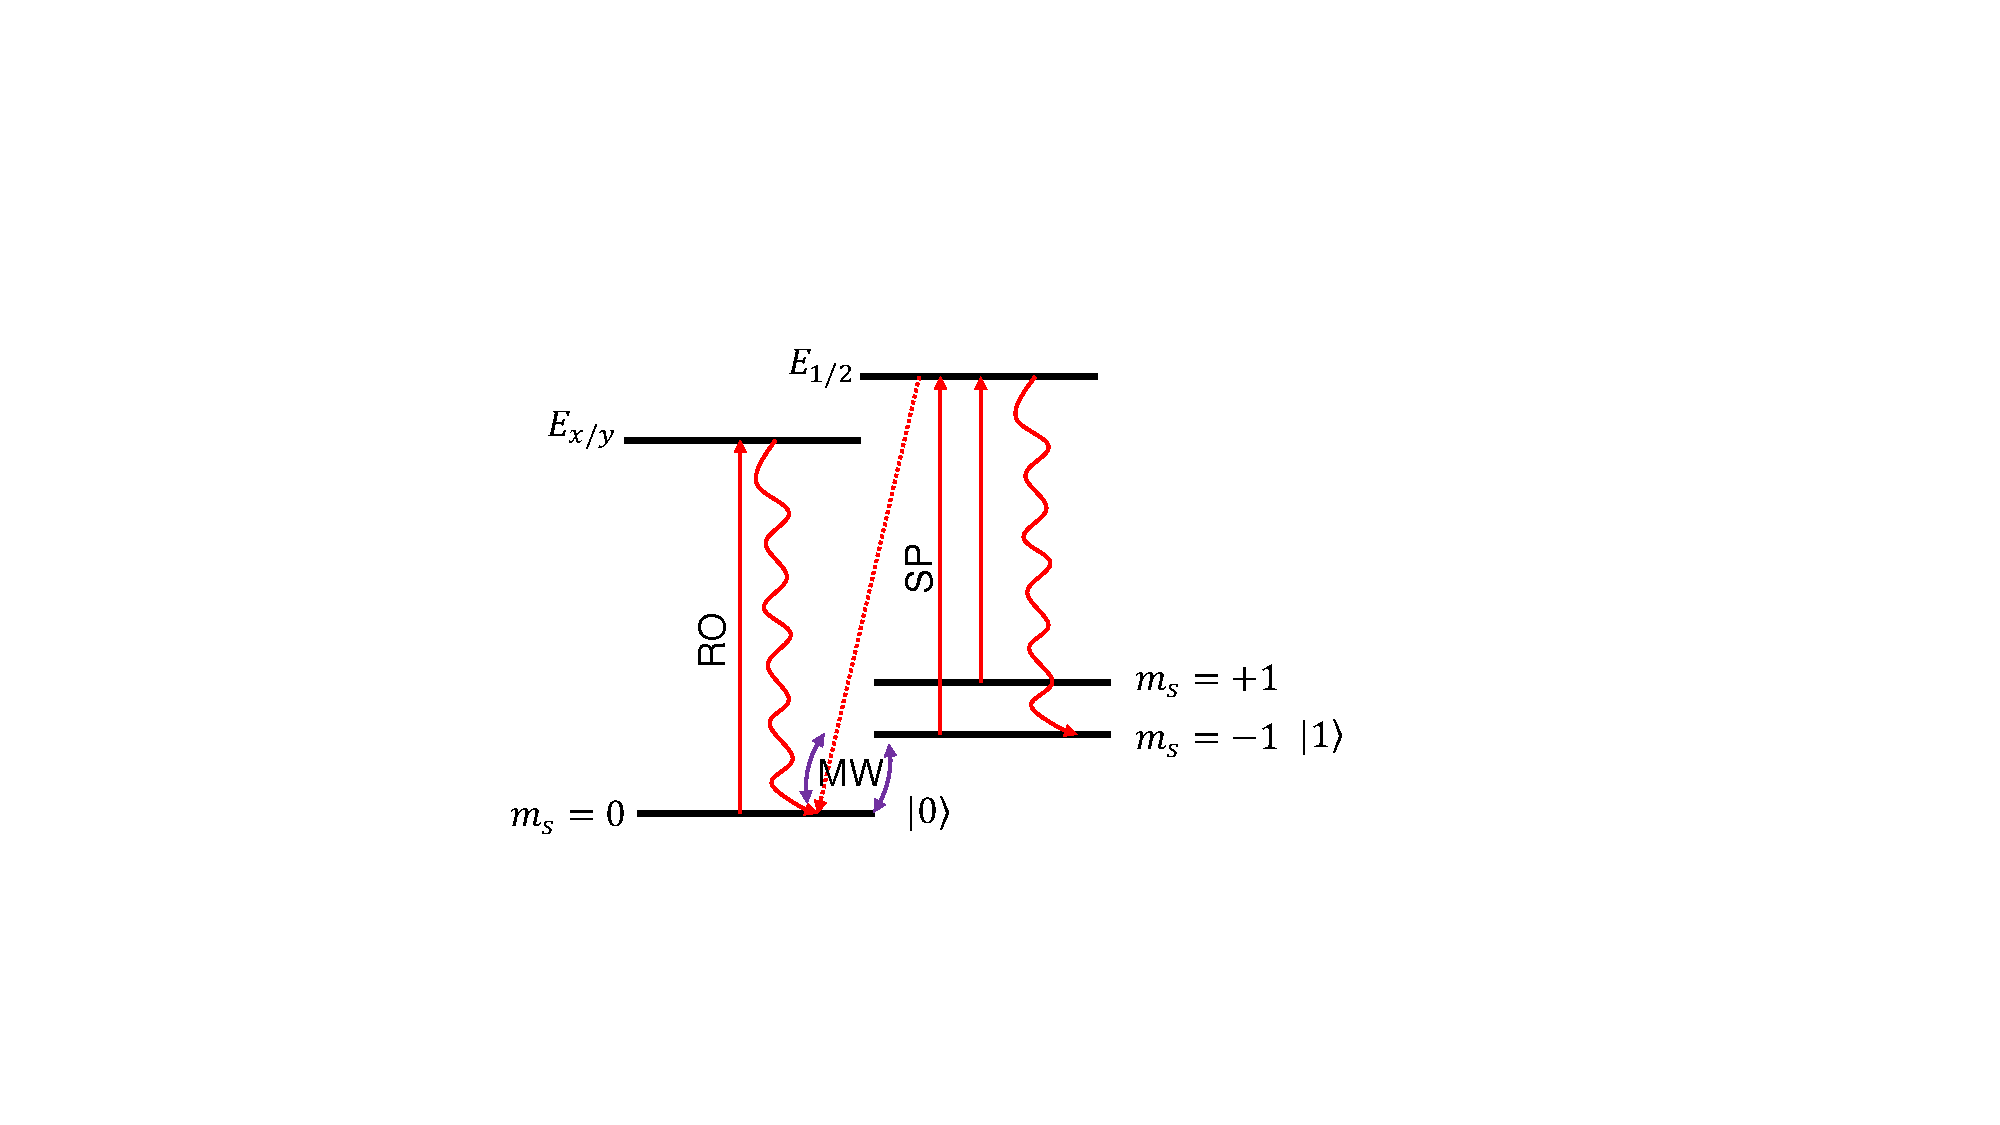
\includegraphics[width=0.8\textwidth]{figures/qnodeos/supplementary/levels_NV.pdf}
    \caption{Energy structure of \ac{NV}$^-$ at 4\,K. The ground state of the \ac{NV} splits into three distinct levels (Zeeman splitting). The optical transitions are spin-selective. The excited states are represented as one, but they are non-degenerate when lateral strain is applied. We denote as \acf{RO} the transition $\ket{0}\rightarrow E_{x/y}$ and as \acf{SP} the transition $\ket{1}\rightarrow E_{1/2}$. The wiggly lines represent the photoluminescence when such transitions are excited, whereas the dashed lines represent the decay via metastable states that is used for initialization of the qubit state into $\ket{0}$. \acf{MW} pulses enables the transfer of population between the two states of the qubit, allowing for quantum information processing.}
    \label{qnodeos:fig:nv_levels}
\end{figure}

In our demonstration, the server has an external magnetic field of $B_z=189$\,mT aligned along the symmetry axis $z$ of the \ac{NV}, while the client experiences $B_z=23$\,mT. The magnetic field is applied via permanent magnets placed both inside and outside the high-vacuum chamber of our closed-cycle cryostats. Fluctuations of the magnetic field are observed on the order of nT on a timescale of hours, therefore they do not constitute a limitation for our demonstration. We also measured a perpendicular component of the permanent magnetic field for both setups of $\sim$1\,mT. Such misalignment becomes crucial for the coherence time of the electron spin qubit, as in the interaction with the surrounding nitrogen nuclear spins, the off-axis hyperfine interaction terms become non-negligible and the decoupling of the electron spin is harder~\cite{doherty_2013}. Notably, the server node is in the regime of ``high magnetic field''. In the level structure depicted in \cref{qnodeos:fig:nv_levels}, this means that the $m_s=-1$ ground state crossed the $m_s=0$ state (at $\sim$\,100mT), and the optical transitions for the \ac{SP} are well separated, such that a double laser field with proper detuning is necessary to correctly address both of them.

\subsubsection{Single Node Operations}

In this section, details on how to operate a single node for quantum information processing are given. The physical setup is the one employed for the demonstration in Ref.~\cite{pompili_2022_experimental}.

\paragraph{Charge-resonance check}

To use the \ac{NV} as a processing node, it is necessary to guarantee that it is in the correct charge state and the laser fields are on resonance with the transitions. Before executing any instructions coming from the \ac{QNPU}, both nodes go through the so-called \ac{CR} check. We apply resonant fields for 100\,$\mu$s on both the \ac{RO} (1\,$n$W) and \ac{SP} (10\,$n$W) transitions and we monitor the fluorescence. If the number of photons exceeds the threshold (25 for the client and 60 for the server for our experiments), the node is considered ready to accept instructions from the \ac{QNPU} and can proceed with synchronization with the other node (for multinode instructions). The threshold is set considering the brightness of each \ac{NV}. The success is considered valid for 100\,$m$s. After this time, if no instructions arrive, the \ac{CR} check is repeated. In case the number of photons is below the threshold, we distinguish two cases: (1) the counts are between the success threshold and a second threshold called Repump: we repeat the \ac{CR} check and tune the frequency of the red lasers, as they might not address the transitions correctly; (2) the number of counts is below the Repump threshold (set at 15 for the client and 25 for the server): this means that the \ac{NV} might be in the dark charge state (\ac{NV}$^{0}$) due to ionization. To restore the charge state, in the next round of \ac{CR} check we first illuminate with off-resonant green laser (20\,$\mu$W for 50\,$\mu$s), or, for the client node only, with yellow light (575\,nm, 35\,$n$W for 300\,$\mu$s) on resonance with the \ac{ZPL} transition of \ac{NV}$^{0}$~\cite{baier_2020}. This is necessary because we additionally apply an external DC field to the \ac{NV} on the client node. We, indeed, exploit the Stark effect to tune the \ac{RO} transition to be the same as the server's one \cite{basssett_2011}. In this way, we can ensure photon indistinguishability in frequency that is crucial for entanglement generation. The typical DC field used for this work is $\sim$2V, modulated via an error signal that is computed on the \ac{CR} check counts, acting as a \ac{PID} loop.

The \ac{CR} check is repeated after an experiment iteration. This round is utilized to validate the experiment and post-select the results based on success or failure of this procedure, as discussed in \cref{qnodeos:sec:methods}.

\paragraph{Single qubit gates}

To manipulate the state of the electron spin qubit, microwave pulses are on resonance with the transition $\ket{0}\rightarrow\ket{1}$ are employed. For the server node, the $m_s=-1$ state is used as $\ket{1}$ and the resonance frequency is 2.4\,GHz. The client node utilizes the $m_s=+1$, with a resonance frequency of 3.5\,GHz. The choice of the $\ket{1}$ is made based on the gate fidelity.

We use skewed-Hermite \acf{MW} pulses~\cite{warren_1984,vandersypen_2005} with high Rabi frequency ($\sim$10\,MHz), which generates an alternating magnetic field capable of manipulating the state of the qubit. The characterizing values for the two nodes are reported in \cref{tab:mw_pulse}. The measured infidelity on a single \ac{MW} pulse is below 1\%. Instructed by the \ac{QNPU}, we performed local quantum tomography on both the server and the client, showing high fidelity. One example is reported in \cref{qnodeos:fig:tomography-no-multitasking}.

\begin{table}[]
    \centering
    \begin{tabular}{|r|c|c|}
    \hline
 &Client & Server\\
\hline
        Duration $\pi$ rotation & 200\,$n$s & 190\,$n$s\\
        Amplitude $\pi$ rotation & 0.78 & 0.89\\
        Skewness $\pi$ rotation & -1.5e$^{-9}$ & -3.5e$^{-9}$\\
        Duration $\pi/2$ rotation & 150\,$n$s&  100\,$n$s\\
        Amplitude $\pi/2$ rotation & 0.38 & 0.56\\
        Skewness $\pi/2$ rotation & -1.2e$^{-8}$& -7.1e$^{-9}$ \\
        Power & 42\,W & 42\,W\\
        \hline
    \end{tabular}
    \caption{Characterizing values for the \ac{MW} pulses. Other rotation angles have the same duration and skewness as the $\pi$ pulse, and the amplitudes scale accordingly. The rotation axes are obtained by changing the phase of the pulse. With the current setup configuration, only rotations along $\hat{x}$ and $\hat{y}$ axes are feasible, so $\hat{z}$ rotations are compiled as combinations of gates along $\hat{x}$ and $\hat{y}$.}
    \label{tab:mw_pulse}
\end{table}

\paragraph{Dynamical decoupling}

Once \ac{MW} pulses are set up with high fidelity, it is possible to implement \ac{DD} sequences that increase the coherence time of the electron spin qubit. \ac{DD} sequences are especially crucial in our experiments when the latency of the \ac{QNPU} is long (milliseconds timescale), like in the \ac{DQC} demonstration. The characterizing parameter for a \ac{DD} sequence is the time delay between the $X$ and $Y$ pulses. To optimize it, we swept the interpulse delay, at the sample precision of our Arbitrary Waveform Generator (0.42\,$n$s, Zurich Instruments HDAWG), while playing the effective single-qubit computation of the \ac{DQC} protocol instructed by the \ac{QNPU}, as explained in \cref{qnodeos:sec:methods}, on both the client and the server. In doing so, we added an extra waiting time of 5\,$m$s between the initialization of the qubit into the superposition state and the subsequent gates to mimic the real-case scenario of the \ac{DQC}. In this way, we are able to set the optimal interpulse delay, obtaining a single-qubit fidelity of 0.96(2) for the server and 0.88(2) for the client.

\paragraph{Single-shot readout}

When a measurement instruction arrives from the \ac{QNPU}, this is translated by the physical layer as a Single-Shot Readout measurement. To assign a state to the qubit, we can use the \ac{RO} optical transition. The \ac{RO} laser field is on for $\sim$10\,$\mu$s at 1\,$n$W. This will produce fluorescence only if the \ac{NV} is in the $\ket{0}$ state. If no photons are detected while the laser is on, the outcome is assigned to the $\ket{1}$ state. The fidelity of the measurement process is defined as $F=1/2(F_{0|0}+F_{1|1})$, where $F_{0|0}$ ($F_{1|1}$) represents the fidelity of measuring $\ket{0}$ ($\ket{1}$) when the qubit is prepared in $\ket{0}$ ($\ket{1}$). For our experiments, we obtain 0.841(4) and 0.997(1) respectively for the client, and 0.912(3) and 0.995(1) for the server, achieving above 0.90 of process fidelity.

\subsubsection{Entanglement generation}
\label{qnodeos:sec:NVentanglement}

The entanglement request from the \ac{QNPU} is translated into executing a single-photon protocol. The communication qubit on each node is initialized in the state $\sqrt{\eta} \ket{0} + \sqrt{1-\eta} \ket{1}$, where $\eta$ represents the bright state population. For maximum state fidelity, the condition $\eta_C p_C \approx \eta_S p_S$ applies, where $\eta_{C(S)}$ is the bright state population of the client (server) and $p_{C(S)}$ is the photon detection probability of the client (server). In this work, $\eta_{C}=0.07$ and $\eta_S = \eta_C \frac{p_C}{p_S} = 0.04$. The choice of $\eta_C$ is a trade-off between entangled state fidelity and entanglement generation rate. The produced entangled state is (non-deterministically) one of two Bell states $\ket{\Psi^\pm} = \frac{1}{\sqrt{2}}(\ket{01} \pm e^{i\Delta\theta}\ket{10})$, based on which detector clicked at the heralding station. The phase $\Delta\theta$ is actively stabilized~\cite{pompili_2021_multinode} before the execution of the entanglement request, via a combination of homodyne interference, for the global phase of the network, and a heterodyne interference, to stabilize the local phase at each node. Pauli-correction gates, based on the state prepared, are issued from the server \ac{QNPU} to its \ac{QDevice} to obtain $\ket{\Phi^+}$: an $X_{\pi}$ gate if the generated Bell-state is $\ket{\Psi^+}$ and an $X_{\pi}$ gate followed by a $Z_{\pi}$ gate (decomposed into X and Y gates) for $\ket{\Psi^-}$. As preparation for the experiment, we verified the entanglement generation, instructed by the \acp{QNPU} and using the same method as in Ref.~\cite{pompili_2022_experimental}, achieving a fidelity of $0.72(\pm 0.02)$ for the $\ket{\Phi^+}$ state. The Bell corrections done through the server \ac{QNPU} take up to 0.16 ms for $\ket{\Psi^+}$ and up to 0.49\,ms for $\ket{\Psi^-}$. On the other hand, generating entanglement without the \ac{QNPU} and with no Pauli correction, we achieve an average fidelity of 0.74($\pm$0.03), with $\eta_{C}=0.1$ and $\eta_S=0.06$. The choice of different $\eta$ values is due, in the first place, to speed up the rate of such a measurement. It shows, however, better performance with respect to the instructed version, which is due to the fact that the Pauli-correction instruction comes with a latency.
\subsection{Trapped-Ion Platform}
\label{sec:trapped-ion-platform}

\subsubsection{Setup}

The trapped-ion \ac{QDevice} implementation faces different challenges than the \ac{NV} \ac{QDevice} implementation. Trapped-ion state preparation, gate operations, and readout occur on longer timescales (between microseconds and milliseconds) than the corresponding operations for \ac{NV} centers. As a result, latencies introduced by \ac{QNodeOS} are insignificant, and we do not expect the use of \ac{QNodeOS} to reduce fidelities of local gate operations or entangling operations on the trapped-ion \ac{QDevice}. On the other hand, trapped ions are typically manipulated using control sequences that are compiled for a given set of parameters and uploaded to hardware. (Here, sequences consist of pulses of \ac{TTL} signals, analog voltages, and radio frequency or microwave signals, some of which are phase-referenced to one another. These pulses typically control the laser and microwave fields with which ions are manipulated.) The challenge here is that decision making within \ac{QNodeOS} must take place further up the network stack and is not compatible with pre-compiled sequences.

We address this challenge by exploiting a triggering capability within our pre-compiled sequences (which are written as Python scripts and then translated to a hardware description language for a \ac{FPGA}). A sequence can contain labels that act as memory pointers; at any point in a given sequence, a function can jump to one of these labels, at which point execution continues starting at that label. Thus, we can structure a sequence as a list of possible subsequences---each of which corresponds to a physical instruction or some part thereof. This list is preceded by a control subsequence. Input triggers from \ac{QNodeOS} cause the control subsequence to jump to a certain subsequence representing a physical instruction. After the subsequence---that is, the physical instruction---is implemented, the sequence returns to the control subsequence, where it waits for another input trigger.

A second challenge is the compatibility between \ac{QNodeOS} and physical-layer hardware. The \ac{QDriver} for \ac{QNodeOS} is implemented with a development \ac{FPGA} board (Texas Instruments LAUNCHXL2-RM57L~\cite{ti_launchxl2_rm57l_2024}) that sends messages via \ac{SPI}. Our physical layer hardware, however, is not compatible with serial communication protocols. We bridge this gap with an emulator board (Cypress, CY8CKIT-14371~\cite{infineon_cy8ckit_143a_2024}). The emulator board requests and reads \ac{SPI} messages from \ac{QNodeOS} and, based on the message, generate \ac{TTL} signals that are sent as input triggers to the physical layer hardware. The emulator also receives outputs from the physical layer hardware: it monitors whether the hardware is available for new commands or busy, and it collects measurement results and passes them back to \ac{QNodeOS}.
In this case, the measurement result consists of \ac{TTL} signals from the \ac{PMT} detecting ion fluorescence. When a counter value on the emulator board exceeds a certain preset threshold, the ion state is registered as the qubit state $\ket{0}$ and otherwise as $\ket{1}$.

\subsubsection{Testing the QDriver}

Tests were carried out using a trapped-ion setup designed for integration with a fiber-based cavity~\cite{teller2023integrating, teller2021heating}. The qubit states consisted of the $4^2 S_{1/2}$ and $3^2 D_{5/2}$ manifolds of $^{40}$Ca$^+$, hereafter referred to as $\ket{0}$ and $\ket{1}$. The cavity was not used in these tests, which focused on single-qubit operations. The cavity was designed to enable ion-photon entanglement, which we plan to implement in future work through physical instructions from \ac{QNodeOS}. Our primary goal in these tests was to verify that the \ac{QNodeOS} hardware, the emulator, and the physical-layer hardware could work together.

Initial tests confirmed that messages were being exchanged at the programmed clock rate of 50\,kHz and that hardware pulses in the physical layer were triggered correctly via the emulator. Next, the following seven tests were implemented:

\begin{enumerate}
\item Initialization of the ion in a specific Zeeman state via Doppler cooling and optical pumping;
\item a bit flip around the X axis via a $\pi$ pulse with phase 0 on the 729\,nm quadrupole transition of $^{40}$Ca$^+$;
\item a bit flip around the Y axis via a $\pi$ pulse with phase $\pi/2$ on the 729 nm transition;
\item preparation of a superposition state via a $\pi/2$ pulse with phase 0 on the 729\,nm transition;
\item readout of a qubit eigenstate in the Y basis via a $\pi$ rotation around X followed by a $\pi/2$ pulse with phase $\pi/2$ around X on the 729\,nm transition;
\item readout of a superposition state in the X basis via a $\pi/2$ rotation around Y followed by a $\pi/2$ pulse around X on the 729\,nm transition;
\item measurement of the ion’s electronic state via fluorescence at 397\,nm in the presence of an 866\,nm repump, following preparation of a superposition state.
\end{enumerate}

Operations are considered to be correctly realized from the point of \ac{QNodeOS}, but do contain errors at the quantum level. Results for the tests (numbers above) were as follows:
%
\begin{enumerate}
\item The ion was detected in the target initial state $\ket{0}$ in 98.4\% of trials;
\item Following the X-axis bit flip operation, the ion was detected in $\ket{1}$ in 96\% of trials;
\item Following the Y-axis bit flip operation, the ion was detected in $\ket{1}$ in 95\% of trials;
\item A projective measurement determined that the $^{40}$Ca$^{+}$ ion was in $\ket{0}$ 52\% of the time and in $\ket{1}$ 48\% of the time;
\item A projective measurement determined that the $^{40}$Ca$^{+}$ ion was in $\ket{0}$ 54\% of the time and in $\ket{1}$ 46\% of the time;
\item The ion was detected in $\ket{0}$ 93\% of the time;
\item The ion population was found to be in $\ket{0}$ 37\% of the time and in $\ket{1}$ 63\% of the time.
\end{enumerate}

These results were consistent with the performance of the physical-layer hardware in the absence of \ac{QNodeOS}. (Note that Doppler cooling had not been optimized and that magnetic-field drifts at the time were not properly compensated for. Gate operations with much higher fidelities are typically achieved in trapped-ion experiments, but here our focus was on verifying the electronic signaling.) No problems or inconsistencies with the electronic signaling were identified. 

A next step will be to implement a more sophisticated processing of \ac{PMT} \ac{TTL} signals by the emulator board in order to identify when the ion has been delocalized due to a background-gas collision; in that case, additional laser cooling will be implemented that returns the ion to Doppler-limited temperatures. Such a step is a typical part of compiled physical-layer sequences but should now be implemented within \ac{QNodeOS} as part of the physical instruction for qubit initialization.
\clearpage
\section{Delegated Quantum Computation (DQC) experiment on NV}
\label{sec:delcomp}

\subsection{Procedure}

We execute the application in a tomography way to establish \ac{QNodeOS} the quantum performance metric (\cref{fig:fig3}b, where we use $P_c$ to refer to the client program, and $P_s$ to the server program): The client \ac{CNPU} initiates $P_c$ with fixed $(\alpha, \theta)$. This results in a single \ac{CNPU} process, a single \ac{QNPU} process, and opening of an \ac{ER} socket (see \cref{sec:design_er_socket}) with the server node. At the same time, the server \ac{CNPU} initiates $P_s$ resulting in single \ac{CNPU} process, a single \ac{QNPU} process, and opening of an \ac{ER} socket with the client node. The client and the server programs execute the subroutines in \cref{fig:fig3}c, looping 1200 times: both immediately start the second iteration once the first is completed. After the 1200th iteration, both client and server stop their respective \ac{CNPU} and \ac{QNPU} processes. Source code including compiled NetQASM subroutines is available in \cref{sec:app_source}. We repeat 6 times for $(\alpha, \theta) \in \{\pi/2, \pi\} \times \{\pi/4, \pi/2, \pi\}$ for a total of 7200 executions of the circuit depicted in \cref{fig:fig3}a. We expect $\ket{\psi}$ to be either $\ket{-Y}$ (for $\alpha = \pi/2$) or $\ket{-Z}$ (for $\alpha = \pi$). To estimate the resulting $\ket{\psi}$ per $(\alpha, \theta)$, the contents of S2 (containing the server qubit measurement) in the server loop is was varied such that we obtained 600 measurement outcomes in basis $\ket{+Y}$ ($\ket{+Z}$) and 600 measurement outcomes in the corresponding orthogonal basis $\ket{-Y}$ ($\ket{-Z}$) for $\alpha = \pi/2$ ($\pi$).

Since our experiments are conducted on two \ac{NV} nodes that are directly connected, we install a constant network schedule with time-bins of 10\,ms in which all time-bins are assigned to networking. This allows us to assess the performance of executing quantum network applications without introducing a dependence on changing network schedules. This means the network process is made ready at the start of each such time-bin, although may not instruct the \ac{QDevice} to make entanglement if no requests for entanglement have been made.

\subsection{Definitions}

The result of a single \ac{DQC} circuit execution (\cref{fig:fig3}a) is a single-qubit state $\rho_{\text{DQC}}$ on the server. The success of running \ac{DQC} can be expressed as the fidelity of $\rho_{\text{DQC}}$ compared to the expected state (in case of no noise) $\ket{\psi}$ (\cref{fig:fig3}a). In the following we will call this fidelity the \ac{DQC} fidelity, or $F_{\text{DQC}}$.

The value of $F_{\text{DQC}}$ is affected the most by (1) the fidelity $F_{\text{EPR}}$ of the entangled pair created between the client and server, and (2) the \textit{qubit memory time} $t_{\text{mem}}$, which is the time that the server qubit must remain in memory (from entanglement success until measurement). The latter depends on the time at which the client sends a message to the server (\cref{fig:fig3}). We refer to the two-qubit maximally entangled Bell states as $\ket{\Phi^+} = \left(\ket{00} + \ket{11}\right)$, and $\ket{\Psi^{\pm}} = \left(\ket{01} \pm \ket{10}\right)$, where $\Phi^+ = \proj{\Phi^+}$ and $\Psi^{\pm} = \proj{\Psi^{\pm}}$.

\subsection{Post-Selection Based on Latency}
\label{sec:post-selection-latency}

In our experiments, the server qubit memory time $t_{\text{mem}}$ has a significant variance across executions of the \ac{DQC} circuit. In some iterations, there were huge spikes in latencies, which skew the results significantly. An upper bound $t_{\max}$ (see \cref{sec:dqc-simulation}) was used to filter out results from iterations in which $t_{\text{mem}}$ was larger than $t_{\max}$. This resulted in filtering 146 out of 7200 data points. We note that for computing $F_{\text{DQC}}$, we applied the latency filter on top of the \ac{SSRO} and \ac{CR} filters (see Methods). For the processing time analysis (below), however, we applied only the latency filter directly to all 7200 original data points.

\subsection{Simulation}
\label{sec:dqc-simulation}

A simulation (using NetSquid~\cite{coopmans_2021_netsquid}) of the \ac{DQC} application was performed in order to estimate the expected $F_{\text{DQC}}$ on our \ac{NV} setup, and to establish a suitable value for $t_{\max}$ (used in latency post-selection).

We emphasize that this simulation is a heuristic to find $t_{\max}$, and does not aim to predict the performance to full accuracy. All runs for which latencies were less than $t_{\max}$ were ultimately used to assess the performance from data, not using this simulation.

The simulation contains the following steps, where we 
used the model explained in Ref.~\cite{pompili_2021_multinode}:
%
\begin{enumerate}
    \item Start with a density matrix $\rho_{\text{EPR}}$ describing the approximate state of the \ac{EPR} pair just after entanglement success.
    \item Apply operations representing the local gates on both the client and server, including the measurement on the client qubit. These operations are assumed to be perfect (no noise).
    \item Apply depolarizing noise to the server qubit for a duration of $t_{\text{mem}}$, using the decoherence formula $e^{-\left(t_{\text{mem}}/T_{\text{coh}}\right)^n}$ where $T_{\text{coh}}$ was set to 13\,ms and $n=1.67$. These values are obtained via fitting experimental data from prior tests.
    \item Calculate the fidelity between the final server qubit state and the expected state $\ket{\psi}$.
\end{enumerate}

Based on the parameters of the setup when the \ac{DQC} experiment was performed, $\rho_{\text{EPR}}$ is set to
%
\[
\begin{bmatrix}
0.049 & 0 & 0 & 0 \\
0 & 0.437 & 0.284 & 0 \\
0 & 0.284 & 0.454 & 0 \\
0 & 0 & 0 & 0.061 \\
\end{bmatrix}
\]
%
which has fidelity 0.729 to the perfect $\Psi^+$ state. The setup can also produce $\Psi^-$ states but for simplicity we use only the $\Psi^+$ case here. 

The simulation computes an estimate of $F_{\text{DQC}}$ for a given server qubit memory time $t_{\text{mem}}$. Since the desired minimum value for $F_{\text{DQC}}$ was 0.667, the latency threshold $t_{\max}$ was set to 8.95\,ms (\cref{fig:delcomp-fidelity-idle-time}).


\begin{figure*}[htbp]
    \centering
    \subfloat[\centering \label{fig:delcomp-fidelity-idle-time}]{{
        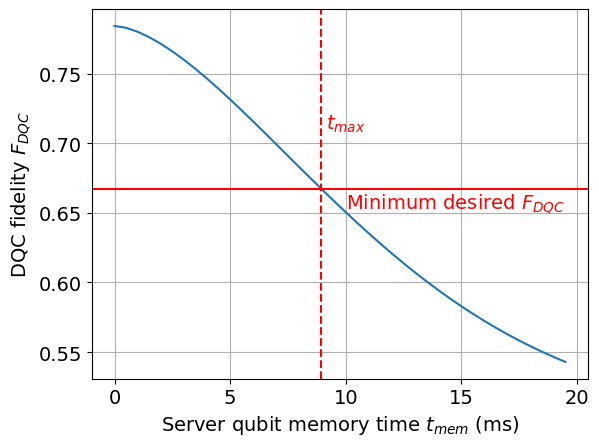
\includegraphics[width=0.48\linewidth]{figures/qnodeos/supplementary/plots/fidelity_vs_idle_time.png}}}%
    \hfill
    \subfloat[\centering \label{fig:delcomp-fidelity-alpha-colormap}]{{
        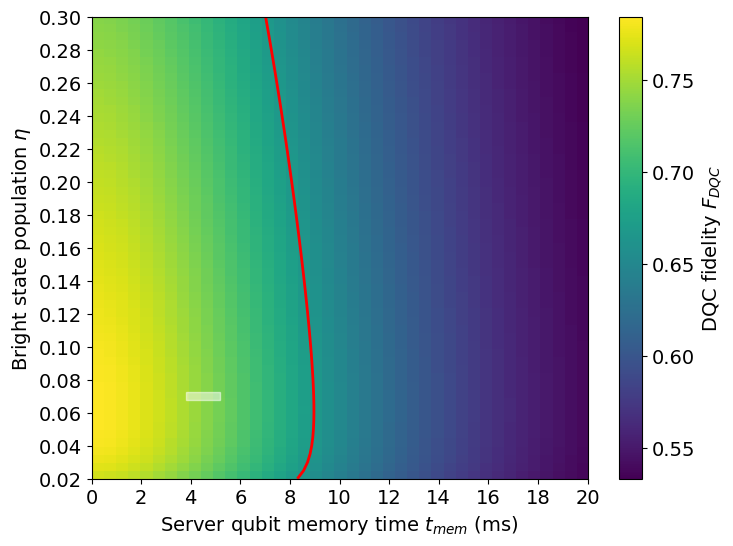
\includegraphics[width=0.48\linewidth]{figures/qnodeos/supplementary/plots/fidelity_eta_colormap.png}}}%
    \caption{
        (a) Expected values (based on simulation, \cref{sec:dqc-simulation}) of \ac{DQC} fidelity $F_{\text{DQC}}$ for different duration values that the server qubit must remain in memory ($t_{\text{mem}}$). The maximum allowed qubit memory time $t_{\max}$ is chosen such that application iterations that are expected to result in too low $F_{\text{DQC}}$ ($<0.667$) are filtered out.
        (b) Expected values (based on simulation) of \ac{DQC} fidelity $F_{\text{DQC}}$ for different values of the bright state population ($\eta$) in the single click protocol, and for different duration values that the server qubit must remain in memory ($t_{\text{mem}}$). The red line indicates the threshold of 0.667 for the target fidelity. The white box represents the experimentally obtained results (we fixed $\eta = 0.07$ and observed $t_{\text{mem}} ~4.8(8)$\,ms, see \cref{fig:fig3}d).
    }
    \label{fig:delcomp-simulation}
\end{figure*}

\subsection{Sweep of Qubit Memory Time and Bright State Population}

As explained in \cref{sec:NVentanglement}, entanglement is created using the single-photon protocol using bright state population parameter $\eta$.\footnote{In most literature, the variable $\alpha$ is used for this parameter; here we use $\eta$ to avoid confusion with the $\alpha$ parameter of the \ac{DQC} application.} Using the simulation, we can estimate how $F_{\text{DQC}}$ would change for different values of $\eta$ and $t_{\text{mem}}$. \cref{fig:delcomp-fidelity-alpha-colormap} shows the estimated $F_{\text{DQC}}$ for different values of $\eta$ and $t_{\text{mem}}$. It indicates that for the particular setup used, increasing $\eta$ has little effect, while reducing qubit memory time does. For the \ac{DQC} experiment $\eta = 0.07$ was used.

\subsection{Processing Time and Latencies}
\label{sec:processing_time_latencies}

Here we provide a detailed breakdown of the duration of execution phases of the \ac{DQC} application, in order to gain insights into the processing times and latencies of the system for the different components.

\subsubsection{Server qubit memory time}
\label{sec:server-qubit-memory-time}

\Cref{fig:fig3}c shows the duration that the server qubit must remain in memory $t_{\text{mem}}$ while waiting, averaged over all \ac{DQC} circuit iterations that passed the latency filter. \Cref{fig:fig3}d shows the breakdown of $t_{\text{mem}}$ into individual segments of processing on both client and server. In \cref{fig:delcomp-latencies-variance} we show the average duration and the variance of each of these segments. The largest time is spent on preparing S2, which involves running Python code on the \ac{CNPU} and converting this (using Python) into a \ac{NetQASM} subroutine. Caching of the preparation of the \ac{NetQASM} subroutine could significantly speed up this process. In the future, further improvements could include an optimized ahead-of-time compilation step. The large variance is due to the fact that on the \ac{CNPU}, other (background) processes run simultaneously with the \ac{DQC} application process, and there is no precise control over the scheduling of these processes.

\begin{figure*}[htbp]
\centering
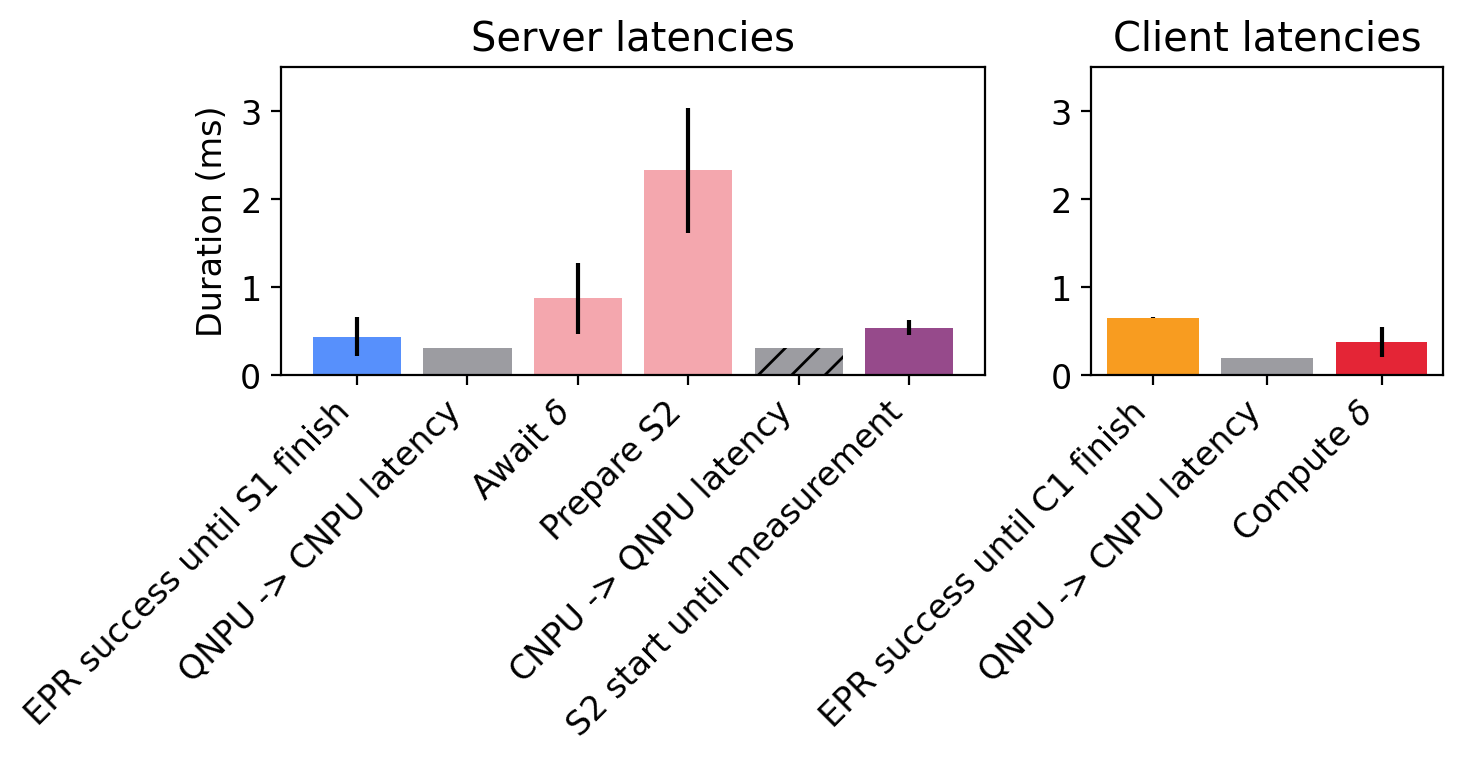
\includegraphics[width=0.8\linewidth]{figures/qnodeos/supplementary/plots/latencies_variance.png}
\caption{Average latency (duration) of each of the processes happening while the server qubit remains in memory in the \ac{DQC} application. The \ac{QNPU} to \ac{CNPU} latency and \ac{CNPU} to \ac{QNPU} latency are estimated as explained in \cref{sec:cnpu-qnpu-latency-estimation}, and fixed to 0.305\,ms (server) and 0.197\,ms (client). The other latencies are the mean and variance of the corresponding processes averaged over all \ac{DQC} circuit iterations that passed the latency filter.}
\label{fig:delcomp-latencies-variance}
\end{figure*}

\subsubsection{Tracing}

The \ac{CNPU}, \ac{QNPU}, and \ac{QDevice} all keep track of events happening in their system, by storing a tuple $(t, e)$ where $t$ is a timestamp and $e$ the name of the event. The events that are traced on the \ac{CNPU} and \ac{QNPU} are listed in \cref{sec:traces}. A trace plot showing events in \ac{CNPU}, \ac{QNPU}, and \ac{QDevice} during a single execution of the \ac{DQC} circuit is also shown in \cref{sec:traces}.

The \ac{QNPU} timestamp granularity is 10\,$\mu$s, since that is the duration of a single \ac{QNPU} clock cycle. This clock cycle is synchronized with the clock of the \ac{QDevice}, which in turn is synchronized with the \ac{QDevice} of the other node (see \cref{sec:methods} and all paragraphs therein related to \ac{NV} implementation). This results in the two \acp{QNPU} (of the two nodes in the experiment) having synchronized clocks with 10\,$\mu$s precision. This means that the event indicating to the \acp{QNPU} that \ac{EPR} generation has succeeded happens at the same clock cycle on both \acp{QNPU}.

The \ac{CNPU} is not a real-time system (instead, it runs on a general purpose Linux \ac{OS}) and records timestamps by consulting the system clock at $\mu$s precision. These timestamps are not synchronized to the \ac{QNPU} timestamps. Furthermore, the \ac{CNPU} timestamps obtained in this way are not as consistent as the real-time clock ticks on the \ac{QNPU}. Therefore, the relative \ac{CNPU} time compared to the \ac{QNPU} time (on the same node) may fluctuate.

% This involves two parts: (1) estimating the global timing offset $G$ between CNPU timestamps and QNPU timestamps, and (2) estimating the latency $L$ between the CNPU and QNPU. The following steps are done:

% \begin{itemize}
%     \item Comparing the difference between the first CNPU \texttt{subroutine sent" event and the first QNPU "subroutine added" event (which should $L + G$)
%     \item Comparing the difference between the first CNPU "result received" event and the first QNPU "subroutine done" event (which should also be $L + G$).
% \end{itemize}

% The average CNPU<->QNPU latency $L$ is then calculated as the average of
% \begin{itemize}
%     \item the global time difference found for the "subroutine send/added" events
%     \item the global time difference found for the "subroutine done/result received" events
% \end{itemize}

\subsubsection{CNPU-QNPU communication latency}
\label{sec:cnpu-qnpu-latency-estimation}

The latency of communication between the \ac{CNPU} and \ac{QNPU} can be calculated by looking at the time between \ac{CNPU} events and \ac{QNPU} events. However, since the \ac{CNPU} timestamps are fluctuating compared to the \ac{QNPU} timestamps, we cannot use a direct comparison between \ac{CNPU} and QNPU timestamps. Instead, we look at time differences on the \ac{CNPU} and compare them to time differences on the QNPU, given that we know the order in which events occur during the DQC application execution. \cref{fig:cnpu_qnpu_latencies} shows a schematic overview of events happening on the \ac{CNPU} and the \ac{QNPU} during a single execution of the \ac{DQC} circuit. By comparing, e.g., (1) the time difference on the \ac{CNPU} between sending subroutine S1 and receiving its result with (2) the time difference on the \ac{QNPU} between receiving subroutine S1 and finishing it, we can estimate the total latency of sending S1 from \ac{CNPU} to \ac{QNPU} and receiving its result. Using this technique, we can estimate the latencies for each communication between \ac{CNPU} and \ac{QNPU}, as listed in \cref{tab:delta_diffs}. Again, since the \ac{CNPU} timestamps fluctuate compared to the \ac{QNPU} timestamps, the derived latencies fluctuate and can even be negative. However, for all derived latencies, we found that a constant function best fit the data. This verifies that the actual latency is constant as expected, and that the variance is due to the inaccuracy of \ac{CNPU} timestamps.

\begin{table*}
    \centering
    \begin{tabular}{|c|c|c|}
    \hline
    \textbf{Derived latency (fit)} & \textbf{Description} & \textbf{Value (ms)} \\ 
    \hline
    $\Delta_{cS1} - \Delta_{qS1}$   & Send S1 + receive S1 result  & $0.384$ \\
    $\Delta_{qS12} - \Delta_{cS12}$ & Receive S1 result + Send S2  & $0.609$ \\
    $\Delta_{cS2} - \Delta_{qS2}$   & Send S2 + receive S2 result  & $0.467$ \\
    $\Delta_{cC1} - \Delta_{qC1}$   & Send C1 + receive C1 result  & $0.394$ \\
    \hline
    \end{tabular}
    \caption{Derived values for \ac{CNPU}-\ac{QNPU} communication latencies. The $\Delta$ variables are observed timestamp differences on the \ac{CNPU} or \ac{QNPU}, per execution of the \ac{DQC} circuit, as shown in \cref{fig:cnpu_qnpu_latencies}. Subtracting pairs of variables from each other produces sums of two \ac{CNPU}-\ac{QNPU} communication latencies. These sums of latencies highly fluctuate per execution of the \ac{DQC} circuit, due to the inaccuracy of the \ac{CNPU} timestamps. However, the data fits a constant value, which is shown in the table and used in further analysis.}
    \label{tab:delta_diffs}
\end{table*}

Using the result from \cref{tab:delta_diffs}, we can compute bounds on the four individual latency variables of the server (we have a system of three linear equations, and we know that all latencies must be strictly non-negative):
%
\begin{itemize}
    \item Sending S1 from \ac{CNPU} to \ac{QNPU}: $<$ 0.242\,ms.
    \item Receiving S1 result on \ac{CNPU} from \ac{QNPU}: between 0.142 and 0.384\,ms.
    \item Sending S2 from \ac{CNPU} to \ac{QNPU}: between 0.225 and 0.467\,ms.
    \item Receiving S2 result on \ac{CNPU} from QNPU: $<$ 0.242\,ms.
\end{itemize}

In the latency breakdown of the server qubit memory time (see \cref{sec:server-qubit-memory-time}) we are only interested in the latencies that happen during the time that the server qubit is in memory. For the server these are the latencies for receiving the S1 result and sending S2. The sum of these two latencies is $\Delta_{qS12} - \Delta_{cS12} = 0.609$\,ms (see \cref{tab:delta_diffs}). For simplicity, we say that both latencies constitute half of this time, as mentioned in the caption of \cref{fig:delcomp-latencies-variance}. Similarly, for the client we are only interested in the latency of receiving the C1 result. For simplicity we take this latency to be the same as that of sending C1, i.e. we use half of $\Delta_{cC1} - \Delta_{qC1}$.

\begin{figure*}[htbp]
    \centering
    \subfloat[\centering \label{fig:subfig3}]{{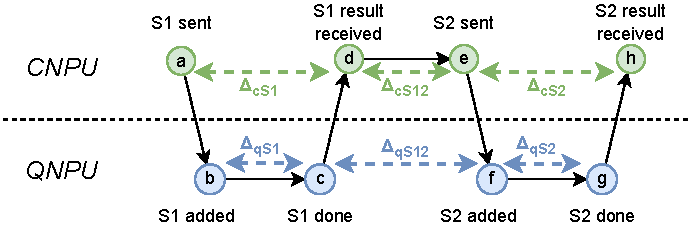
\includegraphics[width=0.61\linewidth]{figures/qnodeos/supplementary/host_qnpu_latency_server.pdf}}}%
    \hfill
    \subfloat[\centering \label{fig:subfig4}]{{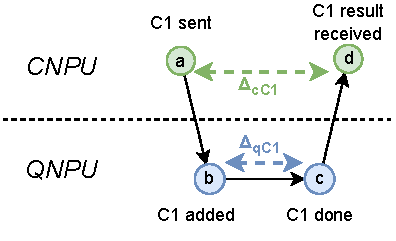
\includegraphics[width=0.35\linewidth]{figures/qnodeos/supplementary/host_qnpu_latency_client.pdf}}}%
    \caption{Schematic of events happening on the \ac{CNPU} and \ac{QNPU} during a single execution of \ac{DQC} on the server (a) and the client (b). Time flows to the right. The $\Delta$ variables are the time differences between events, and are used to estimate \ac{CNPU}-\ac{QNPU} communication latencies ($a\rightarrow b$, $c\rightarrow d$, $e\rightarrow f$, $g\rightarrow h$ on the server and $a\rightarrow b$, $c\rightarrow d$ on the client).}
    \label{fig:cnpu_qnpu_latencies}%
\end{figure*}

\subsubsection{Entanglement generation}

An overview of all values discussed in this section is given in \cref{tab:entanglement_stats}.

\ac{EPR} generation happens by attempting entanglement repeatedly until success. The \ac{QNPU} sends an \texttt{ENT} physical instruction (\cref{tab:qdevice-instructions}) to the \ac{QDevice}, which starts a batch of physical attempts. Each attempt takes 3.95\,$\mu$s and a batch contains 500 attempts. If a batch fails (no success after 500 attempts), the \ac{QNPU} sends another \texttt{ENT} instruction. \cref{tab:entanglement_stats} lists the average success probability per attempt and per batch that we found in the \ac{DQC} experiments. As explained in \cref{sec:NVentanglement}, the \ac{NV} \ac{QDevice} creates either a $\Psi^+$ or a $\Psi^-$ state. \Cref{tab:entanglement_stats} shows statistics on how often each of these states was created during our experiments.

\cref{fig:delcomp-epr-rate} shows the distribution of time it takes to generate an \ac{EPR} pair in the \ac{DQC} experiment, where the average duration of such is 439\,ms. This is the duration between starting the network process and finishing it, which includes entanglement attempts until success on the \ac{QDevice} and subsequent Bell state corrections to $\Phi^+$ (see \cref{sec:qdevice-nv}). This duration corresponds to a fitted rate of 2.28(3) created \ac{EPR} pairs per second. If only the \ac{QDevice} entanglement generation is considered (i.e. without Bell state corrections and without \ac{QNPU} processing overhead), this rate is 2.37(2) \ac{EPR} pairs per second.

\begin{figure}
\centering
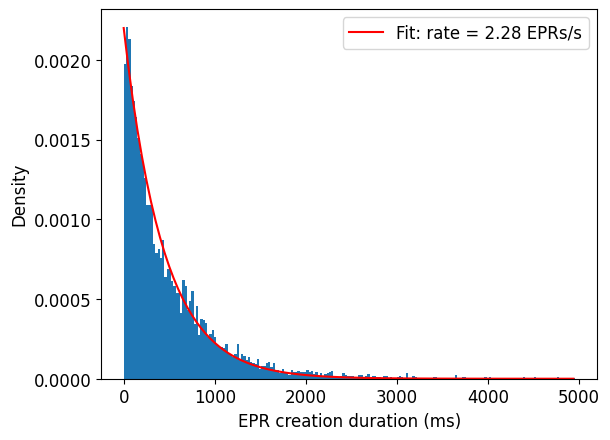
\includegraphics[width=\linewidth]{figures/qnodeos/supplementary/plots/EPR_rate.png}
\caption{Histogram of \ac{EPR} generation durations (time from first attempt until success) based on all \ac{EPR} generations in the \ac{DQC} experiment (using only latency-filtered data points, see \cref{sec:post-selection-latency}). The histogram shows which fraction of all durations were in a particular duration window (window width: 25\,ms). Expected \ac{EPR} generation duration follows an exponential decay, with a rate parameter of 2.28(3) successes (\ac{EPR} pairs) per second.}
\label{fig:delcomp-epr-rate}
\end{figure}

\begin{table*}[htpb]
    \centering
    \begin{tabular}{|r|l|}
    \hline
    \textbf{Parameter} & \textbf{Value} \\ 
    \hline
    Duration of a single entanglement attempt* & 3.95\,$\mu$s \\
    Number of attempts per batch* & 500 \\
    Average number of failed batches until success & 144 \\
    Average success probability per batch & $6.95 \times 10^{-3}$ \\
    Average success probability per attempt & $1.39 \times 10^{-5}$ \\
    Number of Psi+ states generation & 3187 (44.3\%) \\
    Number of Psi- states generation & 4013 (55.7\%) \\
    EPR generation rate (fit) (QDevice) & 2.37(2) EPRs/s \\
    EPR generation rate (fit) (QNodeOS) & 2.28(3) EPRs/s \\
    Average fraction of EPR generation time spent on sync failure & 0.18 \\
    % ...of which client fraction & 0.54 \\
    % ...of which server fraction & 0.46 \\
    
    \hline
    \end{tabular}
    \caption{Overview of values derived from the \ac{DQC} experiment analysis, based on all 7200 \ac{DQC} circuit executions. Entries with an asterisk (*) are values that we fixed in our experiments. The other values are observed experimental results. Average success probabilities are derived from the number of failed batches until success.
    \ac{EPR} generation rate is distinguished between \ac{QDevice} and \ac{QNodeOS}. For the \ac{QDevice}, it indicates the fitted (to an exponential decay function) time between the first \texttt{ENT} physical instruction and the first entanglement success (see \cref{sec:appendix-qdevice}). For \ac{QNodeOS}, it indicates the fitted time between the start of the network process and the end of the network process (i.e. when entanglement has been created and Bell state corrections have been applied, see \cref{sec:qdevice-nv}). Entanglement sync failures happen when one \ac{QDevice} (server or client) wants to attempt entanglement but the other \ac{QDevice} is not ready (\cref{sec:qdevice-sync}). Such sync failures were observed intermittently during a batch of entanglement attempts.}
    \label{tab:entanglement_stats}
\end{table*}

\subsubsection{Local gate durations}

As part of the \ac{DQC} execution, the \ac{QNPU} sends physical instructions to the \ac{NV} \ac{QDevice} for executing local quantum gates. In \cref{tab:gate_durations} we report on the observed durations of these gates from the perspective of the \ac{QNPU}: these durations are from the time the physical instruction is sent to the \ac{QDevice} until the corresponding result is received from the \ac{QDevice}. We note that these durations are longer than these gates would take if they were executed directly on the \ac{QDevice} (without \ac{QNodeOS}, see \cref{tab:mw_pulse}) because of two reasons: (1) the limited granularity with which the \ac{QNPU} and \ac{QDevice} communicate (rounds of 10\,$\mu$s) and (2) the fact the \ac{QDevice} interleaves \ac{DD} sequences in between sequences for the physical instruction itself, as explained in \cref{sec:methods}.

\begin{table*}
    \centering
    \begin{tabular}{|c|c|c|}
    \hline
    \textbf{Physical instruction} & \textbf{Duration (client)} & \textbf{Duration (server)} \\ 
    \hline
    Measure & 130--160\,$\mu$s & 80 - 100\,$\mu$s \\
    X90 & 80--100\,$\mu$s & 50 - 130\,$\mu$s \\
    X180 & 80--100\,$\mu$s & 10 - 130\,$\mu$s \\
    -X90 & --- & 50 - 130\,$\mu$s \\
    Y90 & 70--200\,$\mu$s & 50 - 130\,$\mu$s \\
    Y90 & --- & 50 - 130\,$\mu$s \\
    \hline
    \end{tabular}
    \caption{Duration of executing local quantum gates on the \ac{NV} \ac{QDevice} in the \ac{DQC} experiment. Durations are from sending the physical instruction from \ac{QNPU} to \ac{QDevice} until receiving the \ac{QDevice} response. The -X90 and Y90 gates were never executed in the client \ac{DQC} program.}
    \label{tab:gate_durations}
\end{table*}

\subsubsection{General experiment statistics}

\cref{tab:exp_durations} lists statistics about the overall \ac{DQC} experiment (all 7200 \ac{DQC} circuit executions combined). We confirm our hypothesis that the overwhelming fraction of time is spent on the network process, namely generating \ac{EPR} pairs. We also see that as expected, the server spends more time on user processes than the client does, since it does more local gates than the client (namely, the gates in subroutine S2).

\begin{table*}[htpb]
    \centering
    \begin{tabular}{|r|c|c|}
    \hline
    \textbf{Value} & \textbf{Client} & \textbf{Server} \\ 
    \hline
    Total experiment duration & 4243\,s & 4065\,s \\
    Time spent executing network process & 3840\,s & 3825\,s \\
    Time spent executing user processes & 5.041\,s & 7.618\,s \\
    \hline
    \end{tabular}
    \caption{Overall durations of the \ac{DQC} experiment.}
    \label{tab:exp_durations}
\end{table*}

\subsection{QNPU Network process analysis}

In this section we focus on the execution of the network process in the \ac{QNPU} as observed in the execution of \ac{DQC}. The \ac{ER} sockets~\ref{sec:design_er_socket} are designed to facilitate the generation of entanglement belonging to a pair of user processes between two different \acp{QNPU}. In particular, the \ac{ER} socket allows the \ac{QNPU} to proceed with entanglement generation, while only one node may not have issued a request for entanglement yet. 

During execution of the \ac{DQC} application, the client \ac{QNPU} has a single user process $P_c$ for its \ac{DQC} program and the server \ac{QNPU} has a single user process $P_s$ for its \ac{DQC} program. Both user processes realize the repeated execution of subroutines that jointly realize the \ac{DQC} circuit (\cref{fig:fig3}a).

In each single repetition of the \ac{DQC} circuit, $P_s$ executes first S1 and then S2, and $P_c$ executes C1. $P_s$ (in S1) and $P_c$ (in C1) execute a \ac{NetQASM} instruction for creating an entangled pair, which results in an entanglement request that is submitted to the network stack. Then, $P_c$ and $P_s$ go into the waiting state (see \cref{sec:design:processes}) until the entangled pair is delivered by the network process.

$P_c$ executes a \texttt{create\_epr} instruction and $P_s$ executes a \texttt{recv\_epr} instruction (determined by program source code, see \cref{sec:app_source}. Therefore, the client is seen as the \emph{initiator} (see \cref{sec:design_er_socket}). $P_s$ and $P_c$ open a pair of \ac{ER} sockets with each other when they start and keep it open for the whole experiment. $P_c$ and $P_s$, being on different nodes, operate independently, and may hit their entanglement request instruction at different times. Since the client is the initiator and the server the receiver, the server is always willing to handle an entanglement request with the client. So, the network stack on both client and server will handle a request for entanglement as soon as the client submitted it to its network stack, regardless of whether the server already executed the corresponding \texttt{recv\_epr} in S1.

We observe that in 3245 out of all 7200 \ac{DQC} circuit executions, the client submitted the corresponding entanglement request to its network stack (in C1) \textit{before} the server submitted its entanglement request to its own network stack (in S1), but where the server still complied by starting the network process and handling the request.

\subsubsection{Client waits for server}

From our architecture, we expect that it can happen that the client must wait for the server. This can be the case in the following scenario: The client executes C1 for \ac{DQC} circuit iteration $i$ and submits the entanglement request. Then, the next network time bin starts and the client \ac{QNPU} starts the network process. However, the server is at this time (the beginning of the time bin) still busy with executing S2 for iteration $i-1$ (in user process $P_s$). Therefore the server \ac{QNPU} cannot yet activate its own network process. Since the \ac{ER} socket with the server is open and the client is the `initiator', the client will send entanglement physical instructions to the \ac{QDevice} anyway, but the \ac{QDevice} will not be able to do actual attempts because the server \ac{QDevice} is not ready (\cref{sec:qdevice-sync}). Only when the server \ac{QNPU} completes S2, it can activate the network process, which then sends entanglement physical instructions to the \ac{QDevice}. Only at this point the \acp{QDevice} can start actual entanglement generation. We observe that it did indeed happen that the client had to wait for the server, although we observed this behaviour in only in 60 out of 7200 \ac{DQC} circuit executions.

\subsubsection{Server waits for client}

We expect that it can also happen that the server must wait for the client. This can be the case in the following scenario: The server executes S1 for \ac{DQC} circuit iteration $i$ and submits the entanglement request. Then, the next network time bin starts. However, the client did not yet hit the entanglement request in C1 for \ac{DQC} iteration $i$, so there is nothing to do for the server network process. The server hence needs to wait for the next time-bin, and check again if by now the client has submitted its entanglement request. We observe that in 1323 out of 7200 \ac{DQC} circuit executions, the server had to wait for the client.

\subsubsection{Start of network process}

We examine the start of the network process in relation to the start of a time bin. In particular, the start of the network process may be delayed if there is still a user process running. 

The network process is only activated at the beginning of a time bin. In our experiment, a time bin starts every 10\,ms and lasts 10\,ms. In most cases when the network process is activated, this activation happens very quickly after the time bin start (within 100\,$\mu$s, as some \ac{QNPU} software processing is needed). For the client \ac{QNPU}, the network process never starts more than 100\,$\mu$s after a time bin start. For the server, in 13 out of 7200 \ac{DQC} circuit executions, the network process starts more than 100\,$\mu$s after a time bin starts, since in these cases there was still a user process running. In \cref{tab:network_process_stats}, an overview of all network process statistics is given.

\begin{table*}
    \centering
    \begin{tabular}{|l|l|}
    \hline
    \textbf{Parameter} & \textbf{Value} \\ 
    \hline
    Number of times server puts \ac{EPR} request to network stack before client & 1774/7200 \\
    Number of times server starts entanglement before putting in \ac{EPR} request & 3245/7200 \\
    Number of times submitted \ac{EPR} request is handled in immediate next time bin & 5523/7200 \\
    Average number of bins that pass before request is handled & 2.33 \\
    Number of times server needs to wait for client & 1323/7200 \\
    Number of times client needs to wait for server & 60/7200 \\
    Number of times client network process starts > 100\,$\mu$s after time bin starts & 0 \\
    Number of times server network process starts > 100\,$\mu$s after time bin starts & 13 \\
    \hline
    \end{tabular}
    \caption{Statistics on the \ac{QNPU} network process behavior during the whole \ac{DQC} experiment, i.e. totalled over all 7200 \ac{DQC} circuit iterations.}
    \label{tab:network_process_stats}
\end{table*}
\clearpage
\section{Multitasking experiments on NV}

The multitasking evaluation was done in two parts:
%
\begin{itemize}
    \item \textbf{Quantum tomography while multitasking}: Executing a single \ac{DQC} application (on client and server) and a single \ac{LGT} application (on client only) where it was verified that the \ac{LGT} application produces expected quantum results (see~\cref{qnodeos:sec:multitasking-tomography}).
    \item \textbf{Scaling the number of applications}: Executing $N$ \ac{DQC} applications and $N$ \ac{LGT} applications, where the classical device utilization metric was compared with a version of \ac{QNodeOS} without multitasking, and where we investigated the behavior of the \ac{QNPU} scheduler on the client in the context of multiple programs (see~\cref{qnodeos:sec:multitasking-scaling}).
\end{itemize}
%
The network schedule was set as in the previous \ac{DQC} experiment for direct comparison.

\subsection{Mocked entanglement}
\label{qnodeos:sec:mocked_entanglement}

For the multitasking evaluation, we focused on the behavior of \ac{QNodeOS}, and opted not to use the standard entanglement generation procedure in our \ac{NV} \acp{QDevice} as done in the \ac{DQC} experiments (\cref{qnodeos:sec:delcomp}) to allow for a simpler experiment. Instead, we used a mocked entanglement generation process on the \acp{QDevice} (executing entanglement actions without entanglement): Weak-coherent pulses on resonance with the \ac{NV} transitions, that follow the regular optical path, are employed to trigger the \ac{CPLD} in the entanglement heralding time-window.

We stress that in our multitasking experiments, the exact same physical instructions are sent to the \ac{QDevice} as would be done when using real entanglement, and the exact same responses are sent back. Therefore, \ac{QNodeOS} needed to perform the same operations (including scheduling decisions) as it would have needed to do with real entanglement. Furthermore, we aimed to keep the rate of entanglement `success' in the \acp{QDevice} the same order of magnitude as that of the \ac{DQC} experiments (10.14\,\acp{EPR}/s compared to 2.37\,\acp{EPR}/s in the \ac{DQC} experiment) by keeping the mean-photon number of the weak-coherent pulse comparable to $p_C$ and $p_S$ (in the order of $\sim10^{-4}$). 

\subsection{Tomography results}
\label{qnodeos:sec:multitasking-tomography}

We perform tomography when not multi-tasking, in order to verify our expectation that multi-tasking should not affect the quantum performance of \ac{LGT}: The tomography results of the \ac{LGT} application in the multitasking scenario are given in \cref{qnodeos:fig:fig4}c. We also ran the same \ac{LGT} application on the client in a non-multitasking scenario. In this case, the client ran the \ac{LGT} application and there was no \ac{DQC} application run at all (the server did nothing). The tomography results of \ac{LGT} for the non-mulitasking scenario are given in \cref{qnodeos:fig:tomography-no-multitasking}. The results are slightly different since the multitasking experiment was done on a different day than the non-multitasking experiment. However, within error bars we verify that multitasking does not affect the quantum performance of the \ac{LGT} application.

\begin{figure}
\centering
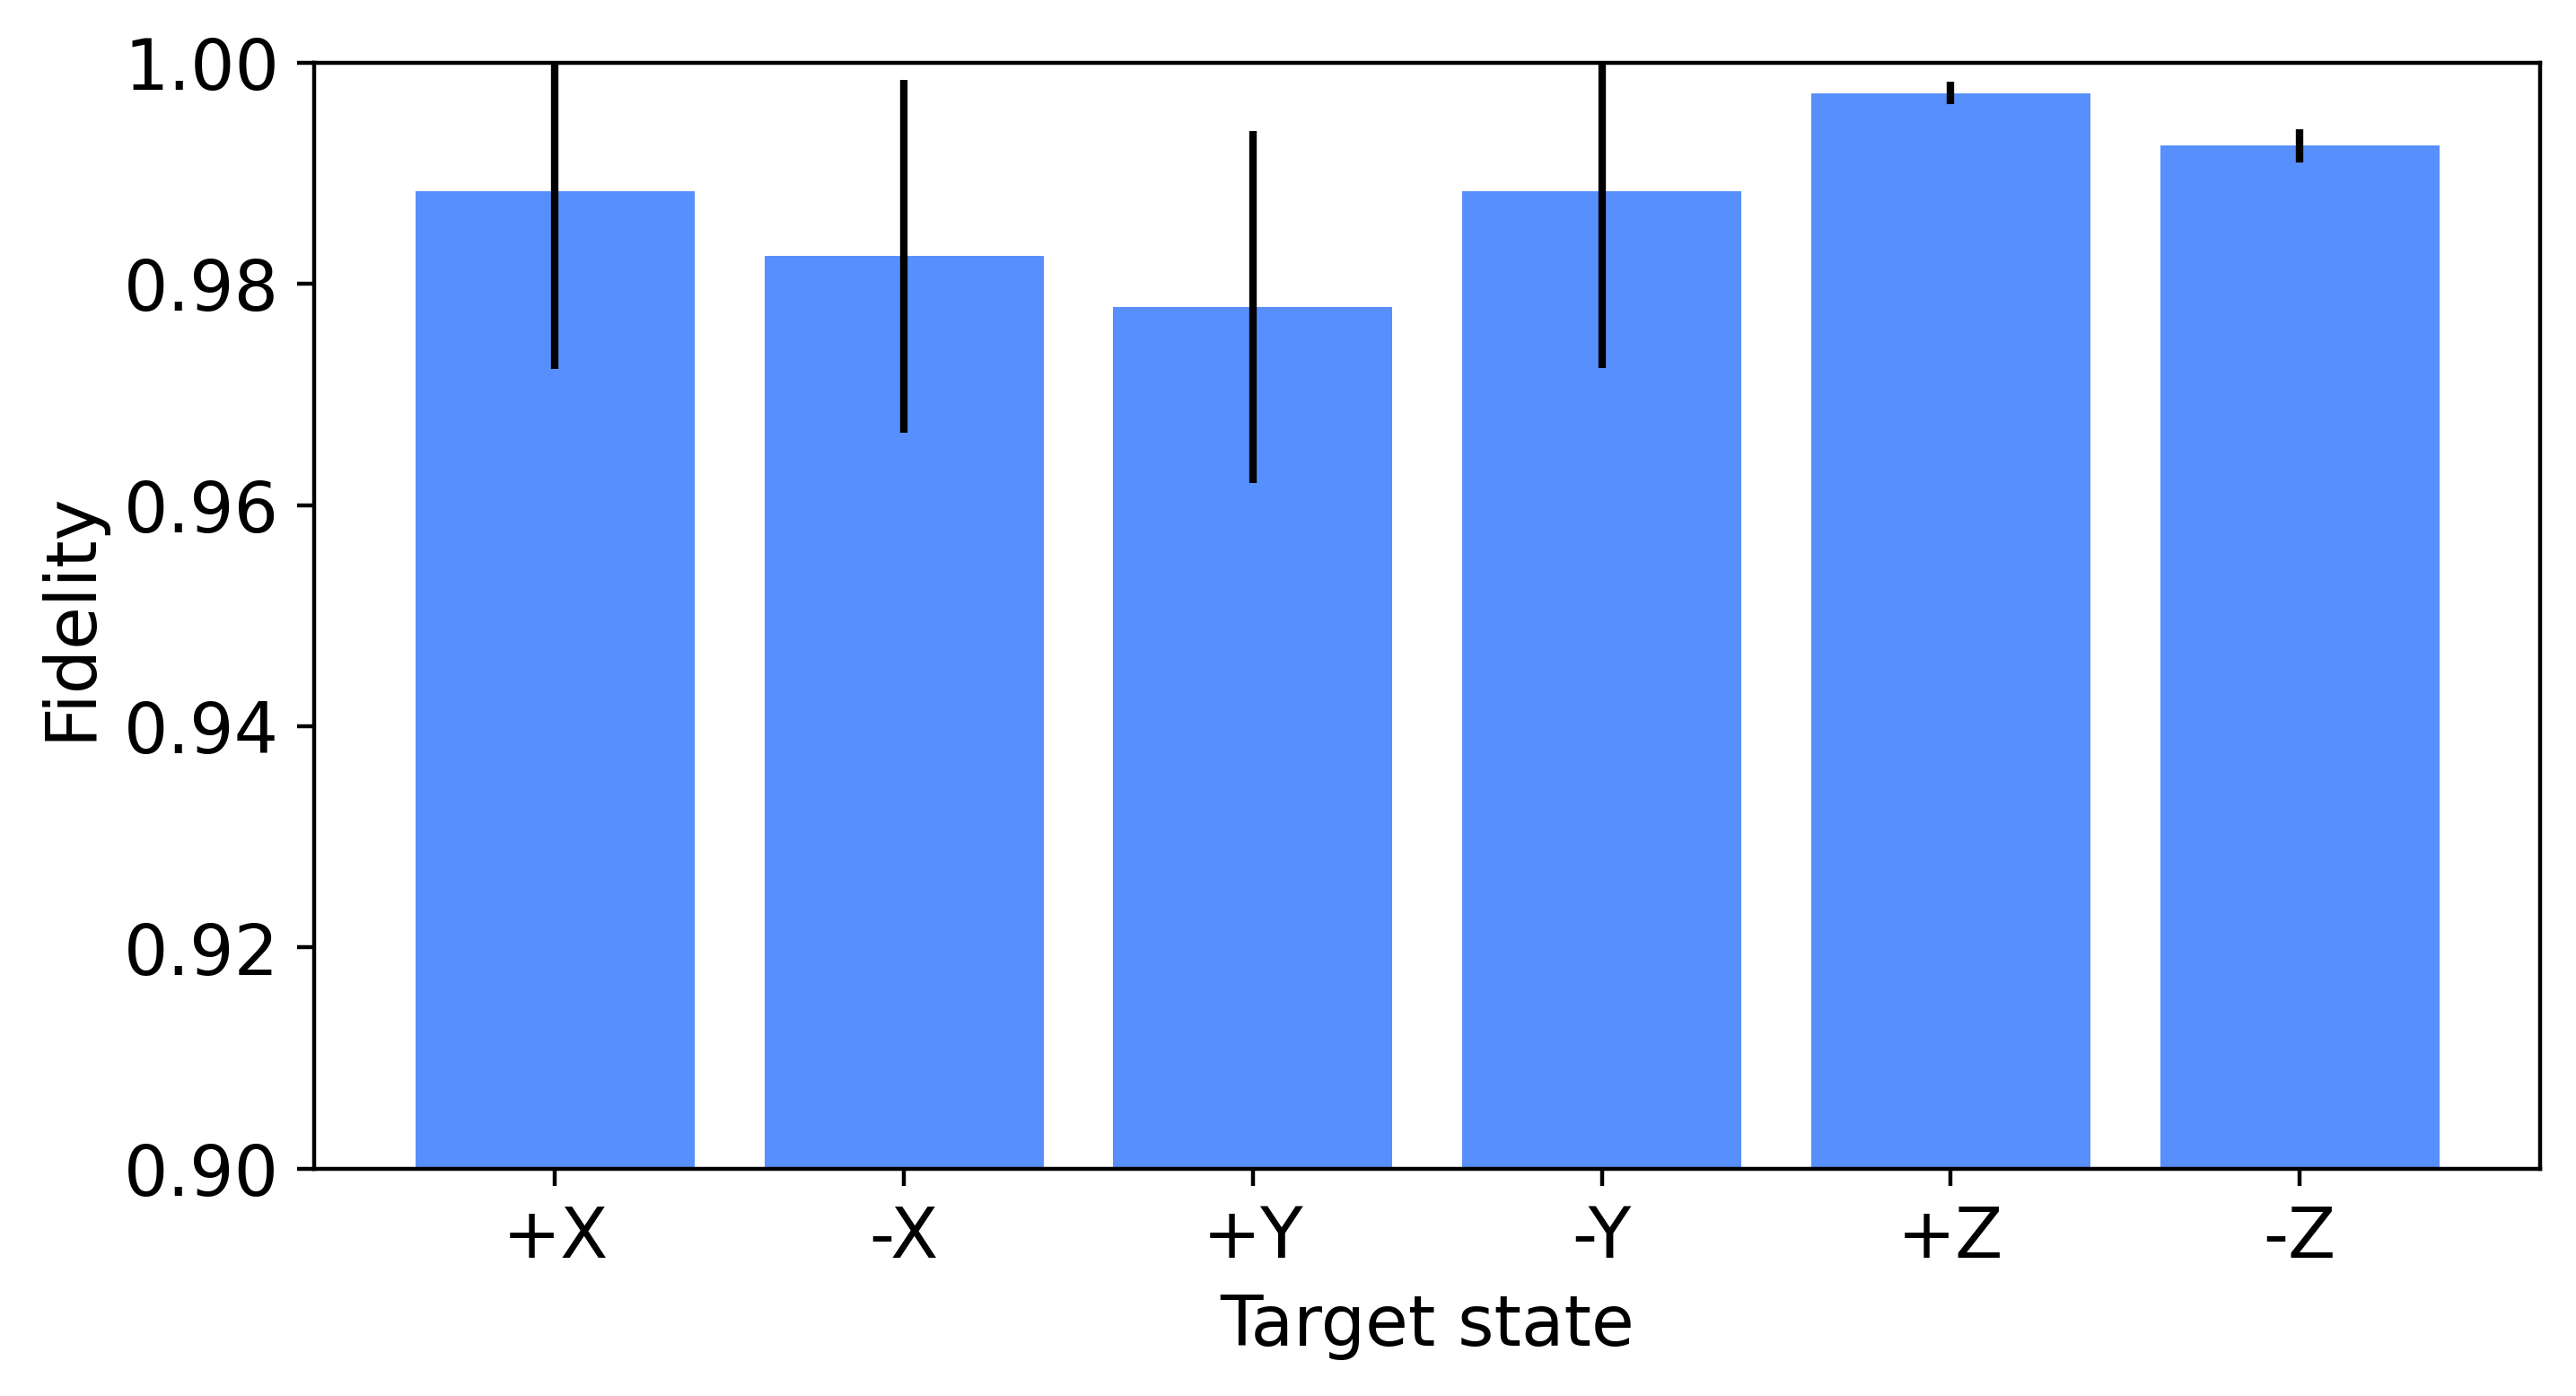
\includegraphics[width=\linewidth]{figures/qnodeos/supplementary/plots/noMT_gate_tomography.png}
\caption{Local Gate Tomography results on the client node in a non-multitasking scenario.}
\label{qnodeos:fig:tomography-no-multitasking}
\end{figure}

\subsection{Scaling to more than two applications}
\label{qnodeos:sec:multitasking-scaling}

\subsubsection{QNPU processes and steps}

For the scaling evaluation, we did an experiment for each $N \in \{1, 2, 3, 4, 5\}$. For each experiment, the client \ac{CNPU} started $N$ \ac{DQC}-client programs and $N$ \ac{LGT} programs concurrently (pseudocode in \cref{src:cnpu_runner}), and the server \ac{CNPU} started $N$ \ac{DQC}-server programs. In this section we discuss the observed behavior of the client and server \acp{QNPU} during these experiments. The client \ac{QNPU} has $2N$ user processes ($N$ \ac{DQC} user processes and $N$ LGT user processes), each of which continuously receives quantum blocks in the form of \ac{NetQASM} subroutines (C1 for \ac{DQC} processes and L1 for \ac{LGT} processes). These $2N$ user processes and the single client network process are scheduled by the client \ac{QNPU} scheduler. The server has $N$ user processes (all for \ac{DQC}) which are scheduled together with the server network process by the server \ac{QNPU} scheduler. \cref{qnodeos:fig:multitasking-default} shows a schematic diagram of the nominal (most often occurring) pattern of scheduling.

In both S1 and C1, there is a single \texttt{create\_epr} \ac{NetQASM} instruction~\cite{dahlberg_2022_netqasm} for creating entanglement with the other node, followed by a \texttt{wait\_all} \ac{NetQASM} instruction that waits until the request entangled qubit is delivered. The \texttt{create\_epr} instruction is handled by the \ac{QNPU} processor by sending the entanglement request to the network stack. Upon executing the \texttt{wait\_all} instruction, the user process executing this subroutine (S1 or C1) goes into the waiting state (green stop sign in \cref{qnodeos:fig:multitasking-default}). When the network process completes (having created the entangled qubit), the user process can be resumed, finishing the subroutine (C1 or S1). 

On the server \ac{QNPU}, for each \ac{DQC} user process $U$ the following sequence is repeated:
%
\begin{itemize}
    \item $U$ is in the \textit{idle} state;
    \item \ac{NetQASM} subroutine S1 is submitted by the \ac{CNPU} to the \ac{QNPU}, moving $U$ to \textit{ready};
    \item $U$ is activated; S1 is executed until it hits the \texttt{wait\_all} instruction; $U$ goes into the \textit{waiting} state;
    \item The network process handles the entanglement request for S1 until \ac{EPR} creation succeeds; $U$ goes into \textit{ready} again;
    \item $U$ is activated; S1 is executed until completion; $U$ goes to \textit{idle};
    \item \ac{NetQASM} subroutine S2 is submitted by the \ac{CNPU}; $U$ goes to \textit{ready};
    \item $U$ is activated; S2 is executed until completion; $U$ goes to \textit{idle}.
\end{itemize}
%
The above sequence is for one execution of the \ac{DQC} circuit (\cref{qnodeos:fig:fig3}a), and is hence repeated many times.

On the client \ac{QNPU}, for each \ac{DQC} user process $U$ the following sequence is repeated:
%
\begin{itemize}
    \item $U$ is in the \textit{idle} state;
    \item \ac{NetQASM} subroutine C1 is submitted by the \ac{CNPU}, moving $U$ to \textit{ready};
    \item $U$ is activated; C1 is executed until it hits the \texttt{wait\_all} instruction; $U$ goes into the \textit{waiting} state;
    \item the network process handles the entanglement request for C1 until \ac{EPR} creation succeeds; $U$ goes into \textit{ready} again;
    \item $U$ is activated; C1 is executed until completion; $U$ goes to \textit{idle}.
\end{itemize}
%
The above sequence is for one execution of the \ac{DQC} circuit (\cref{qnodeos:fig:fig3}a), and is hence repeated many times.

On the client \ac{QNPU}, for each \ac{LGT} user process $U$ the following sequence is repeated:
%
\begin{itemize}
    \item $U$ is in the \textit{idle} state;
    \item \ac{NetQASM} subroutine L1 is submitted by the \ac{CNPU}, moving $U$ to \textit{ready};
    \item $U$ is activated; L1 is executed until completion; $U$ goes to \textit{idle}.
\end{itemize}
%
The above sequence is for one execution of the \ac{LGT} circuit (\cref{qnodeos:fig:fig4}a), and is hence repeated many times.

For the above sequences for user processes, only the internal order is fixed; the time in between steps depends on the \ac{QNPU} scheduler, as well as the time at which the \ac{CNPU} submits subroutines. Furthermore, since there are multiple user processes at the same time (for the server, only for $N > 1$), the above steps happen for each user process $U_i$ and the steps are interleaved. \cref{qnodeos:fig:multitasking-default,fig:multitasking-2-apps,fig:multitasking-wait-on-client} show examples of how these user processes can be interleaved on both client and server \ac{QNPU}.

\subsubsection{DQC and LGT interleaving}

We investigate the degree of interleaving the execution of \ac{DQC} and \ac{LGT}, in particular how many \ac{LGT} subroutines are executed when a \ac{DQC} process is waiting: The client \ac{QNPU} executes both \ac{DQC} and \ac{LGT} user processes. \ac{DQC} user processes are often in the waiting state. This happens when their C1 subroutine is suspended, waiting for the network process to handle their entanglement request. The network process is only activated at the beginning of a time bin, which happens only every 10\,ms, or when a user process finishes executing a subroutine, the latter not occurring very frequently for low number of programs $N$. Furthermore, \ac{DQC} user processes can be in the idle state, namely when they completed execution of C1 for some iteration $i$ of the \ac{DQC} circuit, but are still waiting for the \ac{CNPU} to send C1 for iteration $i+1$. In both these types of `gaps` (waiting or idle), \ac{LGT} subroutines can be executed (each taking $\approx$2.4\,ms). \cref{tab:multitasking_numbers} lists the maximum number of consecutive \ac{LGT} subroutines that were executed in between \ac{DQC} subroutines  for both types of gaps. 

\subsubsection{Subroutine (Quantum block) execution order}

We investigate whether the \ac{QNPU} schedules quantum subroutines in a different order than they arrived from the \ac{CNPU}. As expected, we find that this is the case. Although the \ac{QNPU} handles subroutines from the \ac{CNPU} first-come-first-served, some of these subroutines (in our experiments, precisely the \ac{DQC} subroutines that wait for entanglement) are put into the waiting state. This allows the \ac{QNPU} to schedule other subroutines (in our experiments, we observe \ac{LGT} subroutines being executed), even if they arrived later from the \ac{CNPU} than the waiting \ac{DQC} subroutine. Schematic overviews of such scheduling that we observed are depicted in \cref{qnodeos:sec:multitasking_patterns}.

\subsubsection{User process idle times}

We examine the number of times, and the duration, that a user process is idle waiting for submission of a subroutine from the \ac{CNPU} as a function of $N$: A user process is \textit{idle} when there are currently no subroutines associated with the process pending to be executed. This means that the \ac{QNPU} waits, at least for this user process, until the \ac{CNPU} sends the next subroutine for the user process. \cref{tab:multitasking_numbers} lists the number of times and durations of moments at which all client \ac{QNPU} user processes are idle. This number and their durations decrease for larger values of $N$. This is expected since there are more active processes, and hence more subroutines being sent from the \ac{CNPU} for different processes. In most cases, when finishing a subroutine for user process $U$, there is then another user process $U'$ already waiting with another subroutine to execute.

\subsubsection{Network process start delays}

We examine the scheduling behaviour of the network process in relation to user processes. We expect that due to the fact we use a non-preemptive scheduler, a network process may not be activated at the start of a network time bin, due to a user process still being executed. We investigate the occurrence of such events in our multi-tasking experiment, including the delay with which the network process is started in such a scenario (see \cref{tab:multitasking_numbers}): When a user process submits and entanglement request to the network stack, this request is handled at the earliest when the network process is activated. This happens either at the start of the next network time bin, or when a user process finishes a subroutine. Therefore, there is often some time in between submitting the request and the network process handling it. This waiting time is in most cases bounded by 10\,ms, since that is the length of a time bin, and all time bins are assigned to networking in our experiment. However, in some cases the client may still be executing a \ac{LGT} subroutine when a new time bin starts, delaying the start of the network process until this subroutine has finished. We expect however that in all cases, as soon as such an \ac{LGT} subroutine finishes, the \ac{QNPU} scheduler then immediately schedules the network process, and not another \ac{LGT} subroutine. We found that the maximum difference between time bin start and network process start is 2.59\,ms, which verifies that indeed at most one \ac{LGT} subroutine is sometimes executed during a time bin start (\ac{LGT} subroutine execution duration being $\approx$2.4\,ms.)

We remark that with increasing $N$, the network process is delayed more frequently by a \ac{LGT} subroutine. This is expected due to the fact more subroutines from different user processes await execution. Consequently, with increasing $N$ it also happens more frequently that the client and server do not start execution of the network process in the same time-bin (see below).

\subsubsection{Client waits for server and vice versa}

In order to better understand the concurrent execution of multiple applications (here \ac{DQC} and \ac{LGT}) and corresponding programs, we investigate scenarios and times in which the client waits for the server (or vice versa). 

The client and server open an \ac{ER} socket at the beginning of each \ac{DQC} application. So, during runtime, there are $N$ \ac{ER} sockets opened on the server \ac{QNPU} (one for each \ac{DQC} process) and $N$ \ac{ER} sockets opened on the client \ac{QNPU} (one for each \ac{DQC} process). In each \ac{DQC} application, the client \ac{QNPU} user process for that \ac{DQC} application is the `initiator' (see \cref{qnodeos:sec:design_er_socket}). This means that as soon as the client user process submits a request for entanglement (from within C1), both server and client \ac{QNPU} start their network process to handle it (at the start of the next time bin, and provided the network process should not first handle a request from a user process from another \ac{DQC} application).

It can happen that the client \ac{QNPU} and server \ac{QNPU} do not start their network process at the same time bin. This mostly happens when one of the nodes is still busy executing a user process subroutine when a time bin starts, as explained above. If this happens, the \ac{QNPU} that did already start their network process sends entanglement instructions to their \ac{QDevice}, but this will not result in physical entanglement attempts since the other \ac{QDevice} is not available (leading to a entanglement sync failure, see \cref{qnodeos:sec:qdevice-sync}). \cref{tab:multitasking_numbers} lists the number of times that this happened.

For each of the $N$ \ac{DQC} applications that are running on client and server, and for each execution of the \ac{DQC} circuit in those applications, there is a single entanglement request from the client (in C1) and a single entanglement request from the server (in S1). For each of these request pairs, the client at some point starts the network process and handles this request, and the server at some point starts the network process and handles its corresponding request. For each such pair of requests, the following scenarios can happen:
%
\begin{enumerate}
    \item Client and server \ac{QNPU} start their network process in the same time-bin (one of them may start a bit later than the start of the time-bin because it needs to complete a quantum subroutine).
    \item The client starts its network process in time-bin $k$ but the server starts it at some time-bin $>k$. This happens when the server still has a qubit in memory when time-bin $k$ starts. Therefore, the server cannot activate its network process yet. A qubit still being in memory happens when the server \ac{QNPU} has executed S1 for some \ac{DQC} process (which produced an entangled qubit) but has not yet executed S2 (in which the qubit is measured and hence freed).
    \item The server starts its network process in time-bin $k$ but the client starts it at time-bin $k+1$. This happens (although rarely) when the client user process puts the entanglement request to the network stack just before the start of $k$. The server will immediately start attempts at $k$, but the client itself is still processing and `misses' $k$; the client then only starts at time-bin $k+1$.
\end{enumerate}

\cref{tab:multitasking_numbers} lists how often the above scenarios happen for each $N$.

\begin{table*}
    \centering
    \begin{tabular}{|r|c|c|c|c|c|}
    \hline
    \textbf{Parameter} & \textbf{N = 1} & \textbf{N = 2} & \textbf{N = 3} & \textbf{N = 4} & \textbf{N = 5} \\ 
    \hline
    average no. \ac{LGT} subroutines in between any \ac{DQC} subroutines & 0.83 & 1.42 & 1.59 & 1.65 & 1.65 \\
    max no. consecutive \ac{LGT} subroutines in between \ac{DQC} subroutines & 3 & 4 & 6 & 7 & 8 \\
    max no. consecutive \ac{LGT} subroutines when a \ac{DQC} is in waiting state & 2 & 3 & 4 & 4 & 4 \\
    \% of times that $\geq 1$ \ac{LGT} subroutines fills time waiting for time bin  & 56 & 81 & 99 & 99 & 100 \\
    no. times that network process is delayed by a \ac{LGT} subroutine & 88/360 & 212/720 & 554/1080 & 940/1440 & 1170/1800 \\
    no. time windows in which all user processes are idle & 399 & 56 & 4 & 1 & 0 \\
    Average length of idle time window (ms) & 10 & 5.9 & 5.9 & 8.3 & --- \\
    Maximum length of idle time window (ms) & 152 & 31 & 15 & 8.3 & --- \\
    \% client and server start network process at same time bin & 95.8 & 58.2 & 42.1 & 42.4 & 38.5 \\
    \% server started network process 1 time bin after client & 0.8 & 37.9 & 50.1 & 50.9 & 53.1 \\
    % \% server started network process 2 time-bins after client & 0.0 & 3.2 & 5.6 & 4.9 & 6.6 \\
    % \% server started network process $>2$ time-bins after client & 0.0 & 0.1 & 2.1 & 1.7 & 1.9 \\
    \% server started network process $> 1$ time bins after client & 0.0 & 3.3 & 7.7 & 6.6 & 8.4 \\
    \% client started network process 1 time bin after server & 3.3 & 0.6 & 0.1 & 0.1 & 0.0 \\
    \hline
    \end{tabular}
    \caption{Overview of values derived from the multitasking experiments in which $N$ \ac{DQC} applications (on client and server) and $N$ \ac{LGT} applications (client only) were executed concurrently, for $N \in \{1, 2, 3, 4, 5\}$.}
    \label{tab:multitasking_numbers}
\end{table*}




\clearpage
\section{Multitasking scheduling patterns}
\label{sec:multitasking_patterns}

\begin{figure*}[!htb]
\centering
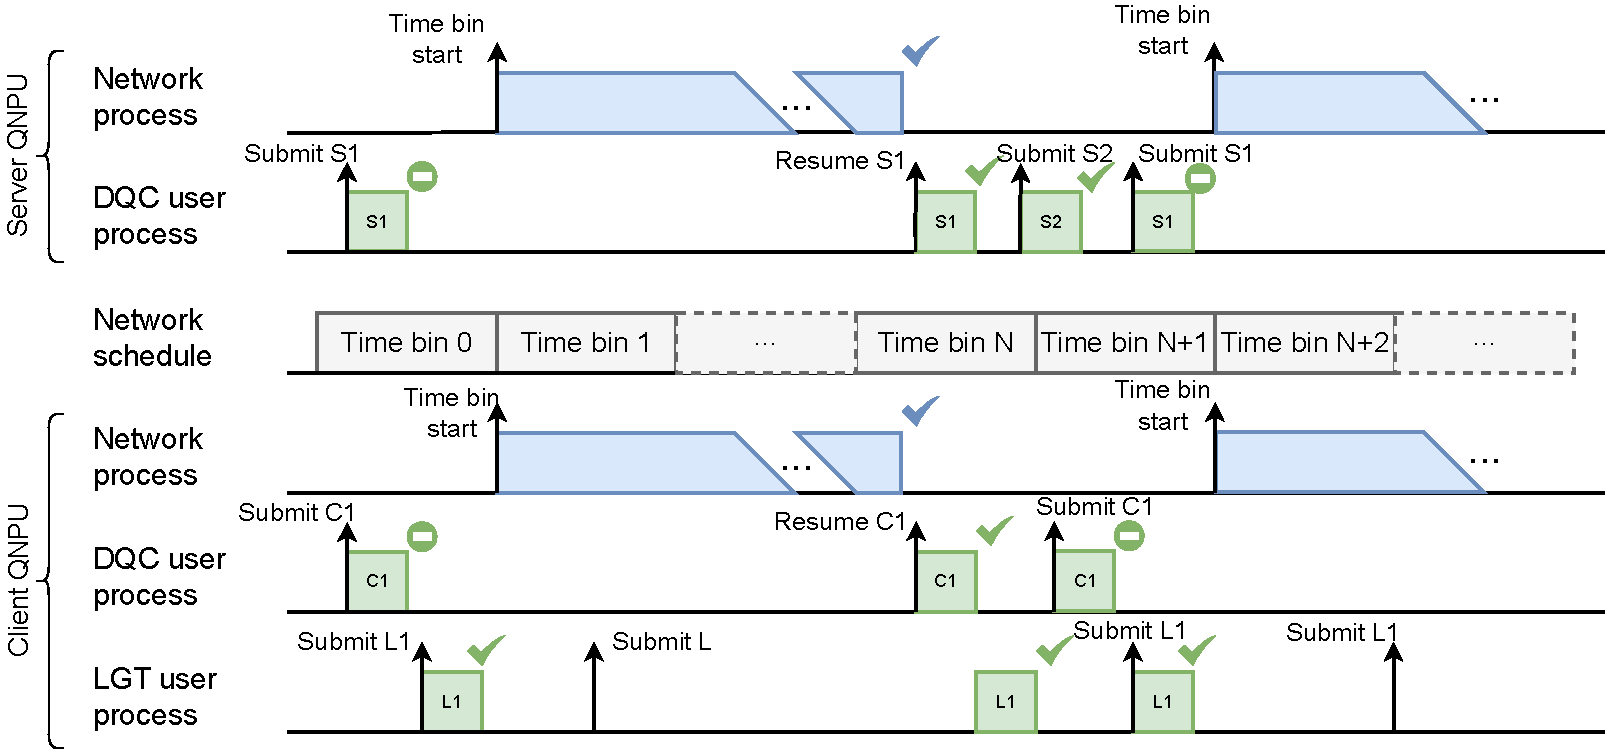
\includegraphics[width=\linewidth]{figures/qnodeos/supplementary/scheduling/MT_default.pdf}
\caption{Nominal scheduling pattern on the client and server \acp{QNPU} when multitasking 1 \ac{DQC} application (on client and server) and 1 \ac{LGT} application (on client only). Pictured is a slice of time (moving to the right) in which a whole \ac{DQC} circuit execution is realized, and 3 \ac{LGT} circuit executions. Up-arrows indicate that the process becomes \textit{ready} (either since a subroutine was submitted from the \ac{CNPU}, or because a requested entangled qubit becomes available). Green blocks are \ac{NetQASM} subroutines. Blue blocks are entanglement generation. Ticks indicate completion of a subroutine (user process) or entanglement request (network process). Stop sign means the user process goes into the \textit{waiting} state. Time not to scale. Time bin length is 10\,ms. Duration of L1 is $\approx$2.4\,ms. Duration of entanglement generation is non-deterministic. On the server \ac{QNPU} the following happens. S1 arrives from \ac{CNPU}; \ac{DQC} user process becomes \textit{ready}. \ac{DQC} user process is activated and executes S1. The entanglement instruction inside S1 is reached; entanglement request is sent to network stack; \ac{DQC} user process becomes \textit{waiting}. When time bin 1 starts, network process becomes \textit{ready}. There is a pending entanglement request, so network process is activated; \ac{QDevice} attempts entanglement until success (after non-deterministic number of time bins, blue tick). Requested entangled qubit is available: \ac{DQC} user process becomes \textit{ready} again; is activated; executes S1 until completion; becomes \textit{idle}. \ac{QNPU} receives subroutine S2 from \ac{CNPU}; activates \ac{DQC} user process; executes S2 until completion. At this point, the \ac{QNPU} completed execution of the current repetition of the \ac{DQC} circuit. \ac{QNPU} then receives again a subroutine S1 (for the next \ac{DQC} circuit iteration), and the same pattern repeats. On the client \ac{QNPU} the following happens. C1 arrives from \ac{CNPU}; \ac{DQC} user process becomes \textit{ready}. \ac{DQC} user process is activated and executes C1. The entanglement instruction inside C1 is reached; entanglement request is sent to network stack; \ac{DQC} user process becomes \textit{waiting}. L1 arrives from \ac{CNPU}; \ac{LGT} user process becomes \textit{ready}. \ac{LGT} user process is activated; fully executes L1. When time bin 1 starts, network process becomes \textit{ready}. There is a pending entanglement request, so network process is activated; \ac{QDevice} attempts entanglement until success (blue tick). While network process is active, another L1 block arrives from \ac{CNPU} (for next \ac{LGT} circuit iteration) so \ac{LGT} user process becomes \textit{ready}. \ac{LGT} user process is not activated since network process is still running. Upon entanglement success, requested qubt is available; \ac{DQC} user process is activated to complete C1. \ac{QNPU} has now completed execution of the current repetition of the \ac{DQC} circuit. \ac{LGT} user process is activated to execute L1 which was still pending. The same pattern repeats.
}
\label{fig:multitasking-default}
\end{figure*}

\clearpage

\begin{figure*}
\centering
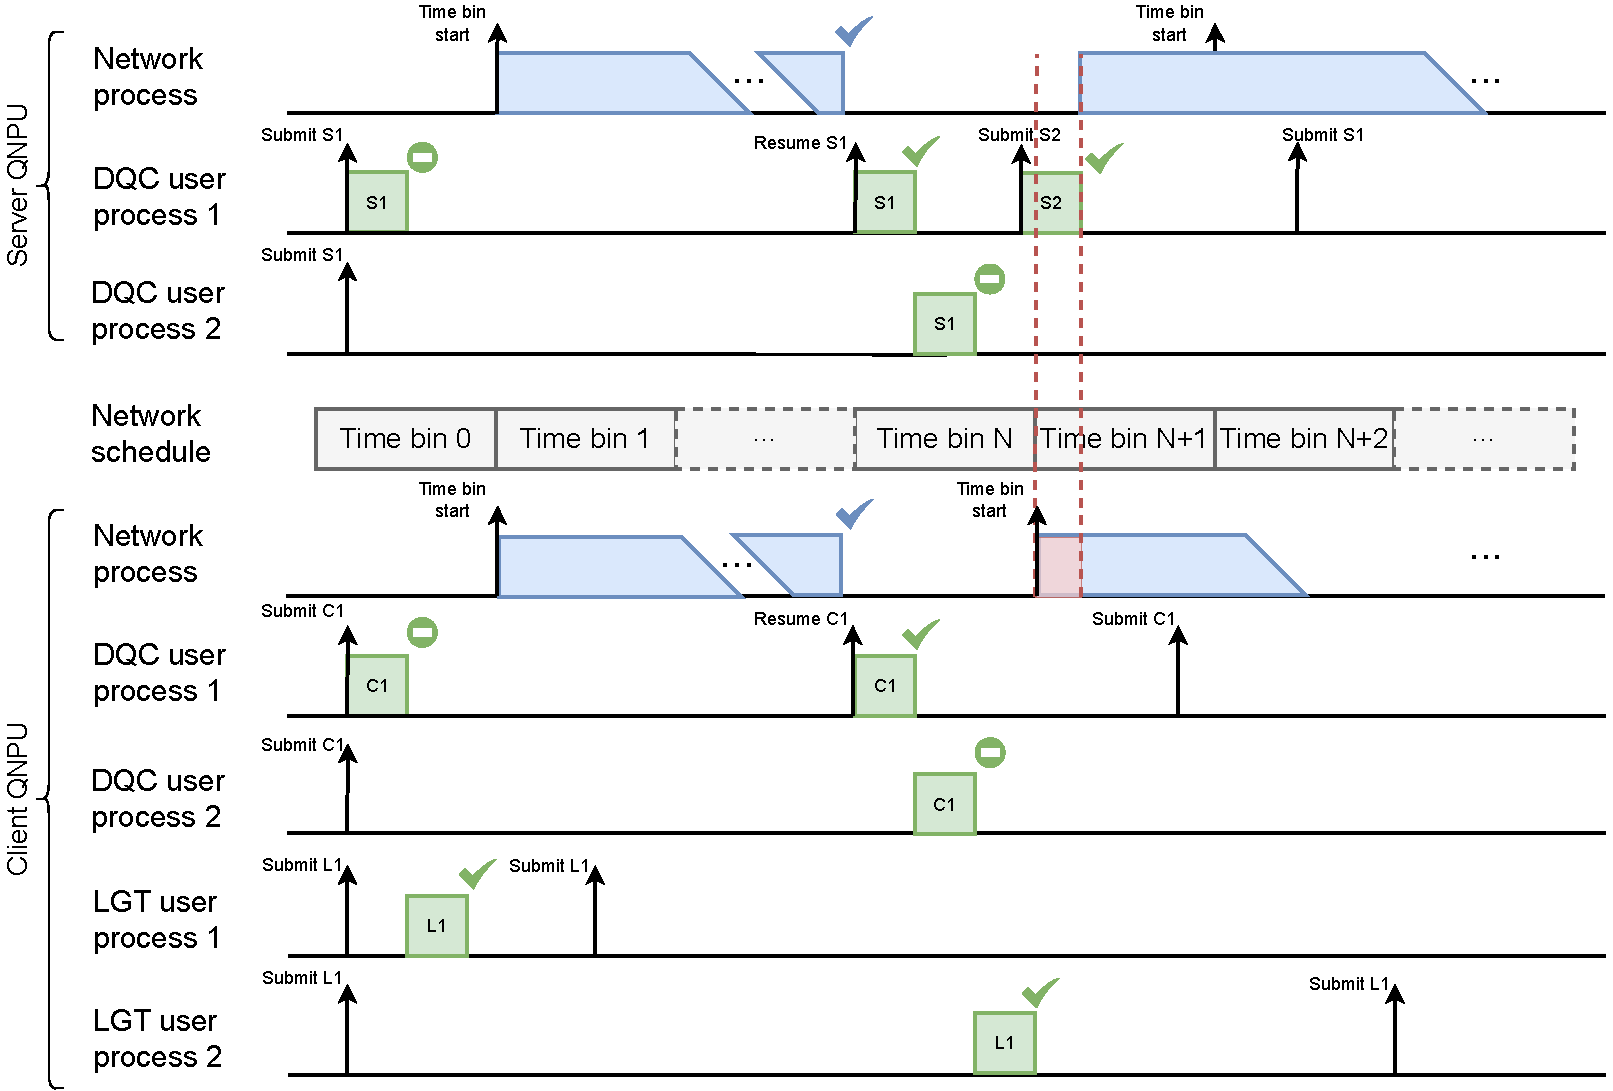
\includegraphics[width=\linewidth]{figures/qnodeos/supplementary/scheduling/MT_2_apps.pdf}
\caption{Example scheduling pattern of scenario with 2 \ac{DQC} applications and 2 \ac{LGT} applications (the symbol and color coding is the same as in~\cref{fig:multitasking-default}). In this case, the client needs to wait (red shared area) for the server to finish S2 of \ac{DQC} user process 1, before they can do entanglement generation for \ac{DQC} user process 2. Scenario: 2 \ac{DQC} applications (A1 and A2) are concurrently executed (A1: \ac{DQC}-server program executed by server \ac{DQC} user process 1 and \ac{DQC}-client program executed by client \ac{DQC} user process 1; A2: \ac{DQC}-server program executed by server \ac{DQC} user process 2 and \ac{DQC}-client program executed by client \ac{DQC} user process 2). Client and server successfully create entanglement for some \ac{DQC} circuit execution $i$ for A1 (just after time bin $N$ starts). Client finishes C1 for user process 1, and meanwhile the server finishes S1 for user process 1. The client has completed its part of \ac{DQC} circuit execution $i+1$ for A1, but the server still needs to wait for S2 from the \ac{CNPU}. Then, the client executes C1 for user process 2, which is the start of circuit execute $j$ for A2; user process 2 becomes waiting. Meanwhile the server executes S1 for user process 2 which becomes waiting. The client needs to wait until the start of the next time bin ($N+1$) until it can activate the network process to handle the request. In the meantime, it can execute an L1 block. Time bin $N+1$ starts and the client handles the request. However, the server has received S2 for execution $i$ of A1, and starts executing it just before the time bin starts. Only after finishing it, the server can start the network process, which picks up the request for A2. While S2 is executing, the client \ac{QDevice} tries to do entanglement attempts, but gets entanglement sync failures~\cref{sec:qdevice-sync} since the server \ac{QDevice} is busy with S2.}
\label{fig:multitasking-2-apps}
\end{figure*}

\clearpage

\begin{figure*}
\centering
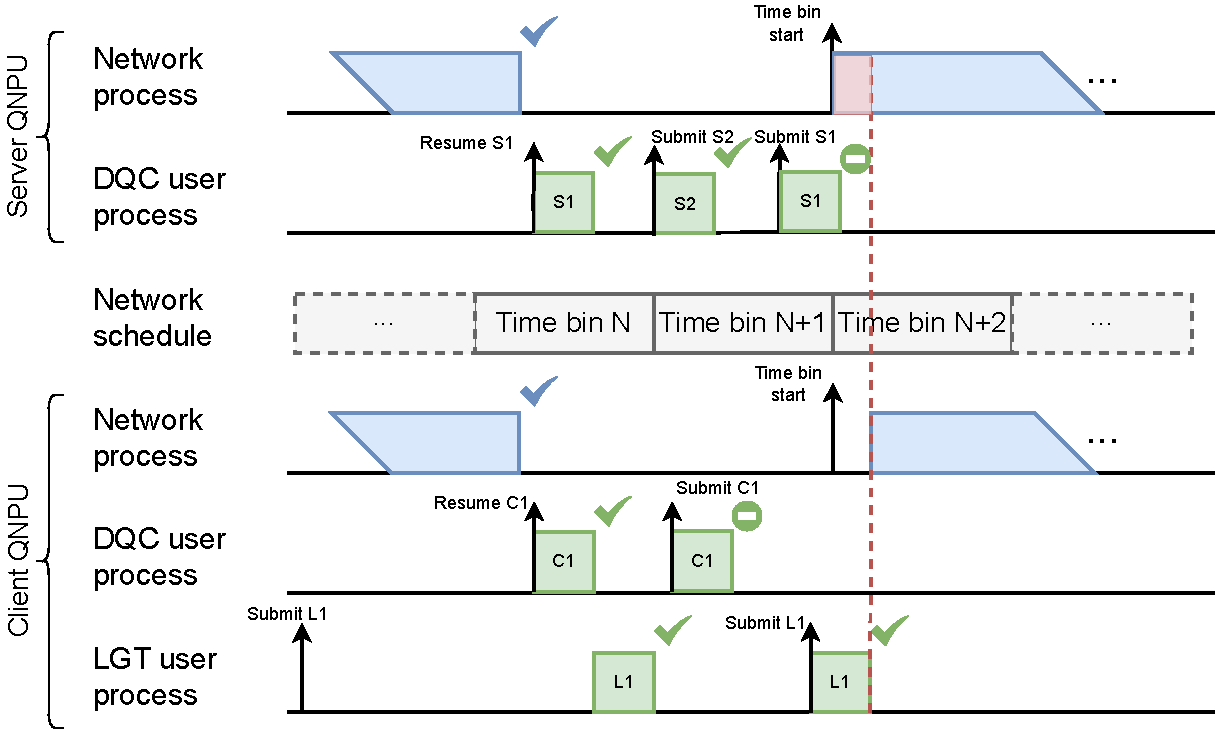
\includegraphics[width=0.8\linewidth]{figures/qnodeos/supplementary/scheduling/MT_wait_on_client.pdf}
\caption{Example scheduling pattern of multitasking one \ac{DQC} application (on client and server) and one \ac{LGT} application (on client only), where the server must wait for client to finish its \ac{LGT} user process (red area); the symbol and color coding is the same as in~\cref{fig:multitasking-default}. At the start of time bin $N+1$, the server activates the network process to handle the request that was put by the previous S1 execution. However the client only starts some time later during the time bin, since it first needs to finish executing L1 for the \ac{LGT} user process.}
\label{fig:multitasking-wait-on-client}
\end{figure*}
\clearpage
\section{Application source code}
\label{sec:app_source}

\begin{figure*}[htbp]
  \centering
  \begin{minipage}{\textwidth}
    \lstinputlisting[language=Python, caption={}]{chapters/main/qnodeos/source/delcomp_server.py}
  \end{minipage}
  \caption{\acf{DQC} source code for the server.}
  \label{src:dqc_server}
\end{figure*}

\clearpage

\begin{figure*}[htbp]
  \centering
  \begin{minipage}{\textwidth}
    \lstinputlisting[language=Python, caption={}]{chapters/main/qnodeos/source/delcomp_client.py}
  \end{minipage}
  \caption{\acf{DQC} source code for the client.}
  \label{src:dqc_client}
\end{figure*}

\clearpage

\begin{figure*}[htbp]
  \centering
  \begin{minipage}{\textwidth}
    \lstinputlisting[language=Python, caption={}]{chapters/main/qnodeos/source/tomography.py}
  \end{minipage}
  \caption{\acf{LGT} source code.}
  \label{src:lgt}
\end{figure*}

\clearpage

\begin{figure*}[htbp]
  \centering
  \begin{minipage}{\textwidth}
    \lstinputlisting[language=Python, caption={}]{chapters/main/qnodeos/source/host_runner.py}
  \end{minipage}
  \caption{Pseudocode illustrating the \ac{CNPU} runner. It can instantiate multiple programs, like the ones defined in~\cref{src:dqc_server,src:dqc_client,src:lgt}. Each program is submitted for concurrent execution to a thread pool executor which is managed by the host \ac{OS}. Each program independently sets up a connection with the \ac{QNPU}, and executes the program code itself.}
  \label{src:cnpu_runner}
\end{figure*}

\lstdefinelanguage{netqasm}
{
    morekeywords={
        add, add, sub, addm, subm,
        jmp, bez, bnz, beq, bne, blt, bge,
        set, store, load, undef, lea,
        array, qalloc, qfree,
        wait_all, wait_any, wait_single,
        ret_reg, ret_arr,
        meas,
        create_epr, recv_epr,
        init, x, y, z, h, s, k, t, rot_x, rot_y, rot_z, cnot, cphase, cx_dir, cy_dir,
        APPID, NETQASM,
    }
    sensitive=false,
    morecomment=[l]{//},
    morecomment=[s]{/*}{*/},
    morecomment=[s][\color{blue}]{\#\ }{\ },
    % morecomment=[s][\color{yellow}]{LOOP}{:},
    morestring=[b]",
}

\clearpage

\begin{figure*}[htbp]
  \centering
  \begin{minipage}{\textwidth}
    \lstinputlisting[basicstyle=\small\ttfamily, language=netqasm, caption={}]{chapters/main/qnodeos/source/dqc_S1.nqasm}
  \end{minipage}
  \caption{\ac{NetQASM} subroutine S1 of the \ac{DQC} application. Compiled by the \ac{DQC} server program code listed in~\cref{src:dqc_server}.}
  \label{src:netqasm_dqc_s1}
\end{figure*}

\clearpage

\begin{figure*}[htbp]
  \centering
  \begin{minipage}{\textwidth}
    \lstinputlisting[basicstyle=\small\ttfamily, language=netqasm, caption={}]{chapters/main/qnodeos/source/dqc_S2.nqasm}
  \end{minipage}
  \caption{\ac{NetQASM} subroutine S2 of the \ac{DQC} application. Compiled by the \ac{DQC} server program code listed in~\cref{src:dqc_server}. The exact gates may differ depending on the iteration of the program loop and the $\delta$ value sent by the client.}
  \label{src:netqasm_dqc_s2}
\end{figure*}

\clearpage

\begin{figure*}[htbp]
  \centering
  \begin{minipage}{\textwidth}
    \lstinputlisting[basicstyle=\small\ttfamily, language=netqasm, caption={}]{chapters/main/qnodeos/source/dqc_C1.nqasm}
  \end{minipage}
  \caption{\ac{NetQASM} subroutine C1 of the \ac{DQC} application. Compiled by the \ac{DQC} client program code listed in~\cref{src:dqc_client}. The exact gates may differ depending on the \ac{DQC} parameters $\alpha$ and $\theta$.}
  \label{src:netqasm_dqc_c1}
\end{figure*}

\clearpage

\begin{figure*}[htbp]
  \centering
  \begin{minipage}{\textwidth}
    \lstinputlisting[basicstyle=\small\ttfamily, language=netqasm, caption={}]{chapters/main/qnodeos/source/lgt.nqasm}
  \end{minipage}
  \caption{\ac{NetQASM} subroutine L1 of the \ac{LGT} application. Compiled by the \ac{LGT} program code listed in~\cref{src:lgt}. The exact gates may differ depending on the iteration of the program loop.}
  \label{src:netqasm_lgt_l1}
\end{figure*}

\clearpage
\section{Traces}
\label{qnodeos:sec:traces}

In our \ac{NV} experiments, the \ac{CNPU}, \ac{QNPU} and \ac{QDevice}, on both client and server nodes, trace (i.e. record the timestamps of) events happening on their system. The events that are traced on the \ac{CNPU} and \ac{QNPU} are listed in~\cref{tab:host_events,tab:qnpu_events}, respectively. The \ac{NV} \ac{QDevice} separately records messages received (physical instructions from the \ac{QNPU}, see~\cref{tab:qdevice-instructions}) and responses sent back to the \ac{QNPU}(see~\cref{tab:qdevice-return-values}).

\Cref{qnodeos:fig:delcomp-trace-example} shows a full-stack trace slice of a single execution of the \ac{DQC} circuit. This particular sequence of events started at offset 60460\,ms from the start of the experiment. The following events (among others) can be seen:
%
\begin{itemize}
    \item At $\approx$\,60470\,ms: client \ac{CNPU} sends subroutine C1 to the \ac{QNPU}; it is received slightly after on the \ac{QNPU} (\texttt{PROCMGR\_SUBROUTINE\_ADDED\_P0}).
    \item Slightly after 60470\,ms: the \ac{QNPU} starts the user process containing C1; it hits the entanglement instruction and moves the process to the waiting state (\texttt{PROCESSOR\_WAIT\_USER\_PROCESS}).
    \item At 60480\,ms: the first next time bin starts, starting the network process on both client and server. This results in \texttt{ENTANGLE} commands being sent to the \acp{QDevice} by both client and server.
    \item Between 60480 and 60550\,ms: the two \acp{QDevice} repeatedly attempt entanglement but fail (each \texttt{ENTANGLE} instruction from the \ac{QNPU} starts one batch; each \texttt{ENTANGLEMENT\_FAILURE} return message indicates the batch failed).
    \item Meanwhile at 60485\,ms, the server \ac{CNPU} sends subroutine S1 to the \ac{QNPU}.
    \item At $\approx$\,60552.5\,ms, the \acp{QDevice} succeed in entanglement generation, producing a $\ket{\Psi^+}$ Bell pair.
    \item After this, the client and server finish C1 and S1, respectively. The client sends instructions for local gates ending with a \texttt{MEASURE} physical instruction. The server starts S1, hits the \texttt{recv\_epr} instruction, goes into the waiting state, gets immediately unblocked (since the entangled pair was already created) and sends a bell state correction gate to the \ac{QDevice} (\texttt{X180}).
    \item At $\approx$\,60553.5\,ms, the client \ac{CNPU} receives the result of C1 (\texttt{RESULT\_RCVD}), and sends the classical message $\delta$ to the server \ac{CNPU} (\texttt{CLAS\_MSG\_SENT}).
    \item At $\approx$\,60554\,ms, the server \ac{CNPU} receives $\delta$ (\texttt{CLAS\_MSG\_RCVD}).
    \item At $\approx$\,60557\,ms, the server \ac{CNPU} sends S2 to the \ac{QNPU}. The \ac{QNPU} executes the user process containing S2 which involves sending local quantum instructions to the \ac{QDevice} ending with a measurement.
    \item At $\approx$\,60558\,ms, the \ac{QNPU} sends the result of S2 to the \ac{CNPU}.
\end{itemize}

\clearpage

\begin{table}[t]
    \centering
    \begin{tabular}{|c|l|}
    \hline
    \textbf{Event name} & \textbf{Description} \\ 
    \hline
    \texttt{SUBROUTINE\_SEND\_ATTEMPT} & Try to send subroutine to \ac{QNPU} \\
    \texttt{SUBROUTINE\_SENT} & Subroutine sent to \ac{QNPU} \\ 
    \texttt{RESULT\_RCVD} & Subroutine results received from \ac{QNPU} \\
    \texttt{CLAS\_MSG\_SENT} & Classical message sent to other node \\
    \texttt{CLAS\_MSG\_RCVD} & Classical message received from other node \\
    \hline
    \end{tabular}
    \caption{\ac{CNPU} events that are traced (recorded with their timestamps) during application execution.}
    \label{tab:host_events}
\end{table}

\begin{table}
    \centering
    \begin{tabular}{|c|l|}
    \hline
    \textbf{Event name} & \textbf{Description} \\ 
    \hline
    \texttt{SCHEDULER\_ARRIVE\_USER\_PROCESS} & A user process goes to the Ready state \\
    \texttt{SCHEDULER\_SCHEDULE\_USER\_PROCESS} & A user process goes to the Running state \\
    \texttt{SCHEDULER\_ARRIVE\_NET\_PROCESS} & Network process goes to the Ready state \\
    \texttt{SCHEDULER\_SCHEDULE\_NET\_PROCESS} & Network process goes to the Running state \\
    \texttt{PROCMGR\_SUBROUTINE\_ADDED\_P<i>} & \makecell[l]{New subroutine received from \ac{CNPU} for \\ process <i>} \\
    \texttt{PROCMGR\_SUBROUTINE\_DONE\_P<i>} & A subroutine for process <i> finished execution \\
    \texttt{PROCESSOR\_START\_USER\_PROCESS} & \makecell[l]{Processor starts or resumes executing a user \\ process} \\
    \texttt{PROCESSOR\_WAIT\_USER\_PROCESS} & \makecell[l]{Processor suspends a user process and puts it \\ in the Waiting state} \\
    \texttt{PROCESSOR\_FINISH\_USER\_PROCESS} & Processor stops executing a user process \\
    \texttt{PROCESSOR\_START\_NET\_PROCESS} & \makecell[l]{Processor starts or resumes executing the \\ network process} \\
    \texttt{PROCESSOR\_FINISH\_NET\_PROCESS} & Processor stops executing the network process \\
    \texttt{QDEVICE\_PRODUCE\_<cmd>\_CMD} & \makecell[l]{Processor prepares <cmd> command for the \\ \ac{QDevice}} \\
    \texttt{QDEVICE\_CONSUME\_CMD} & \makecell[l]{\ac{QDevice} reads the next command from the \\ \ac{QNPU}} \\
    \texttt{QDEVICE\_PRODUCE\_OUTCOME} & \ac{QDevice} sends result to the \ac{QNPU} \\
    \texttt{PROCESSOR\_CONSUME\_OUTCOME} & Processor reads \ac{QDevice} result \\
    \texttt{QNETWORK\_ENT\_PULL} & Network stack pulls instruction from the EGP \\
    \texttt{EGP\_NEI\_OK} & QEGP notifies that EPR pair has been created \\
    \hline
    \end{tabular}
    \caption{\ac{QNPU} events that are traced (recorded with their timestamps) during application execution. <i> can be any number from 0 to 9 (`subroutine added` and `subroutine done` events are not traced for processes with ID 10 or larger). <cmd> can be any physical instruction.}
    \label{tab:qnpu_events}
\end{table}

\begin{figure*}
\centering
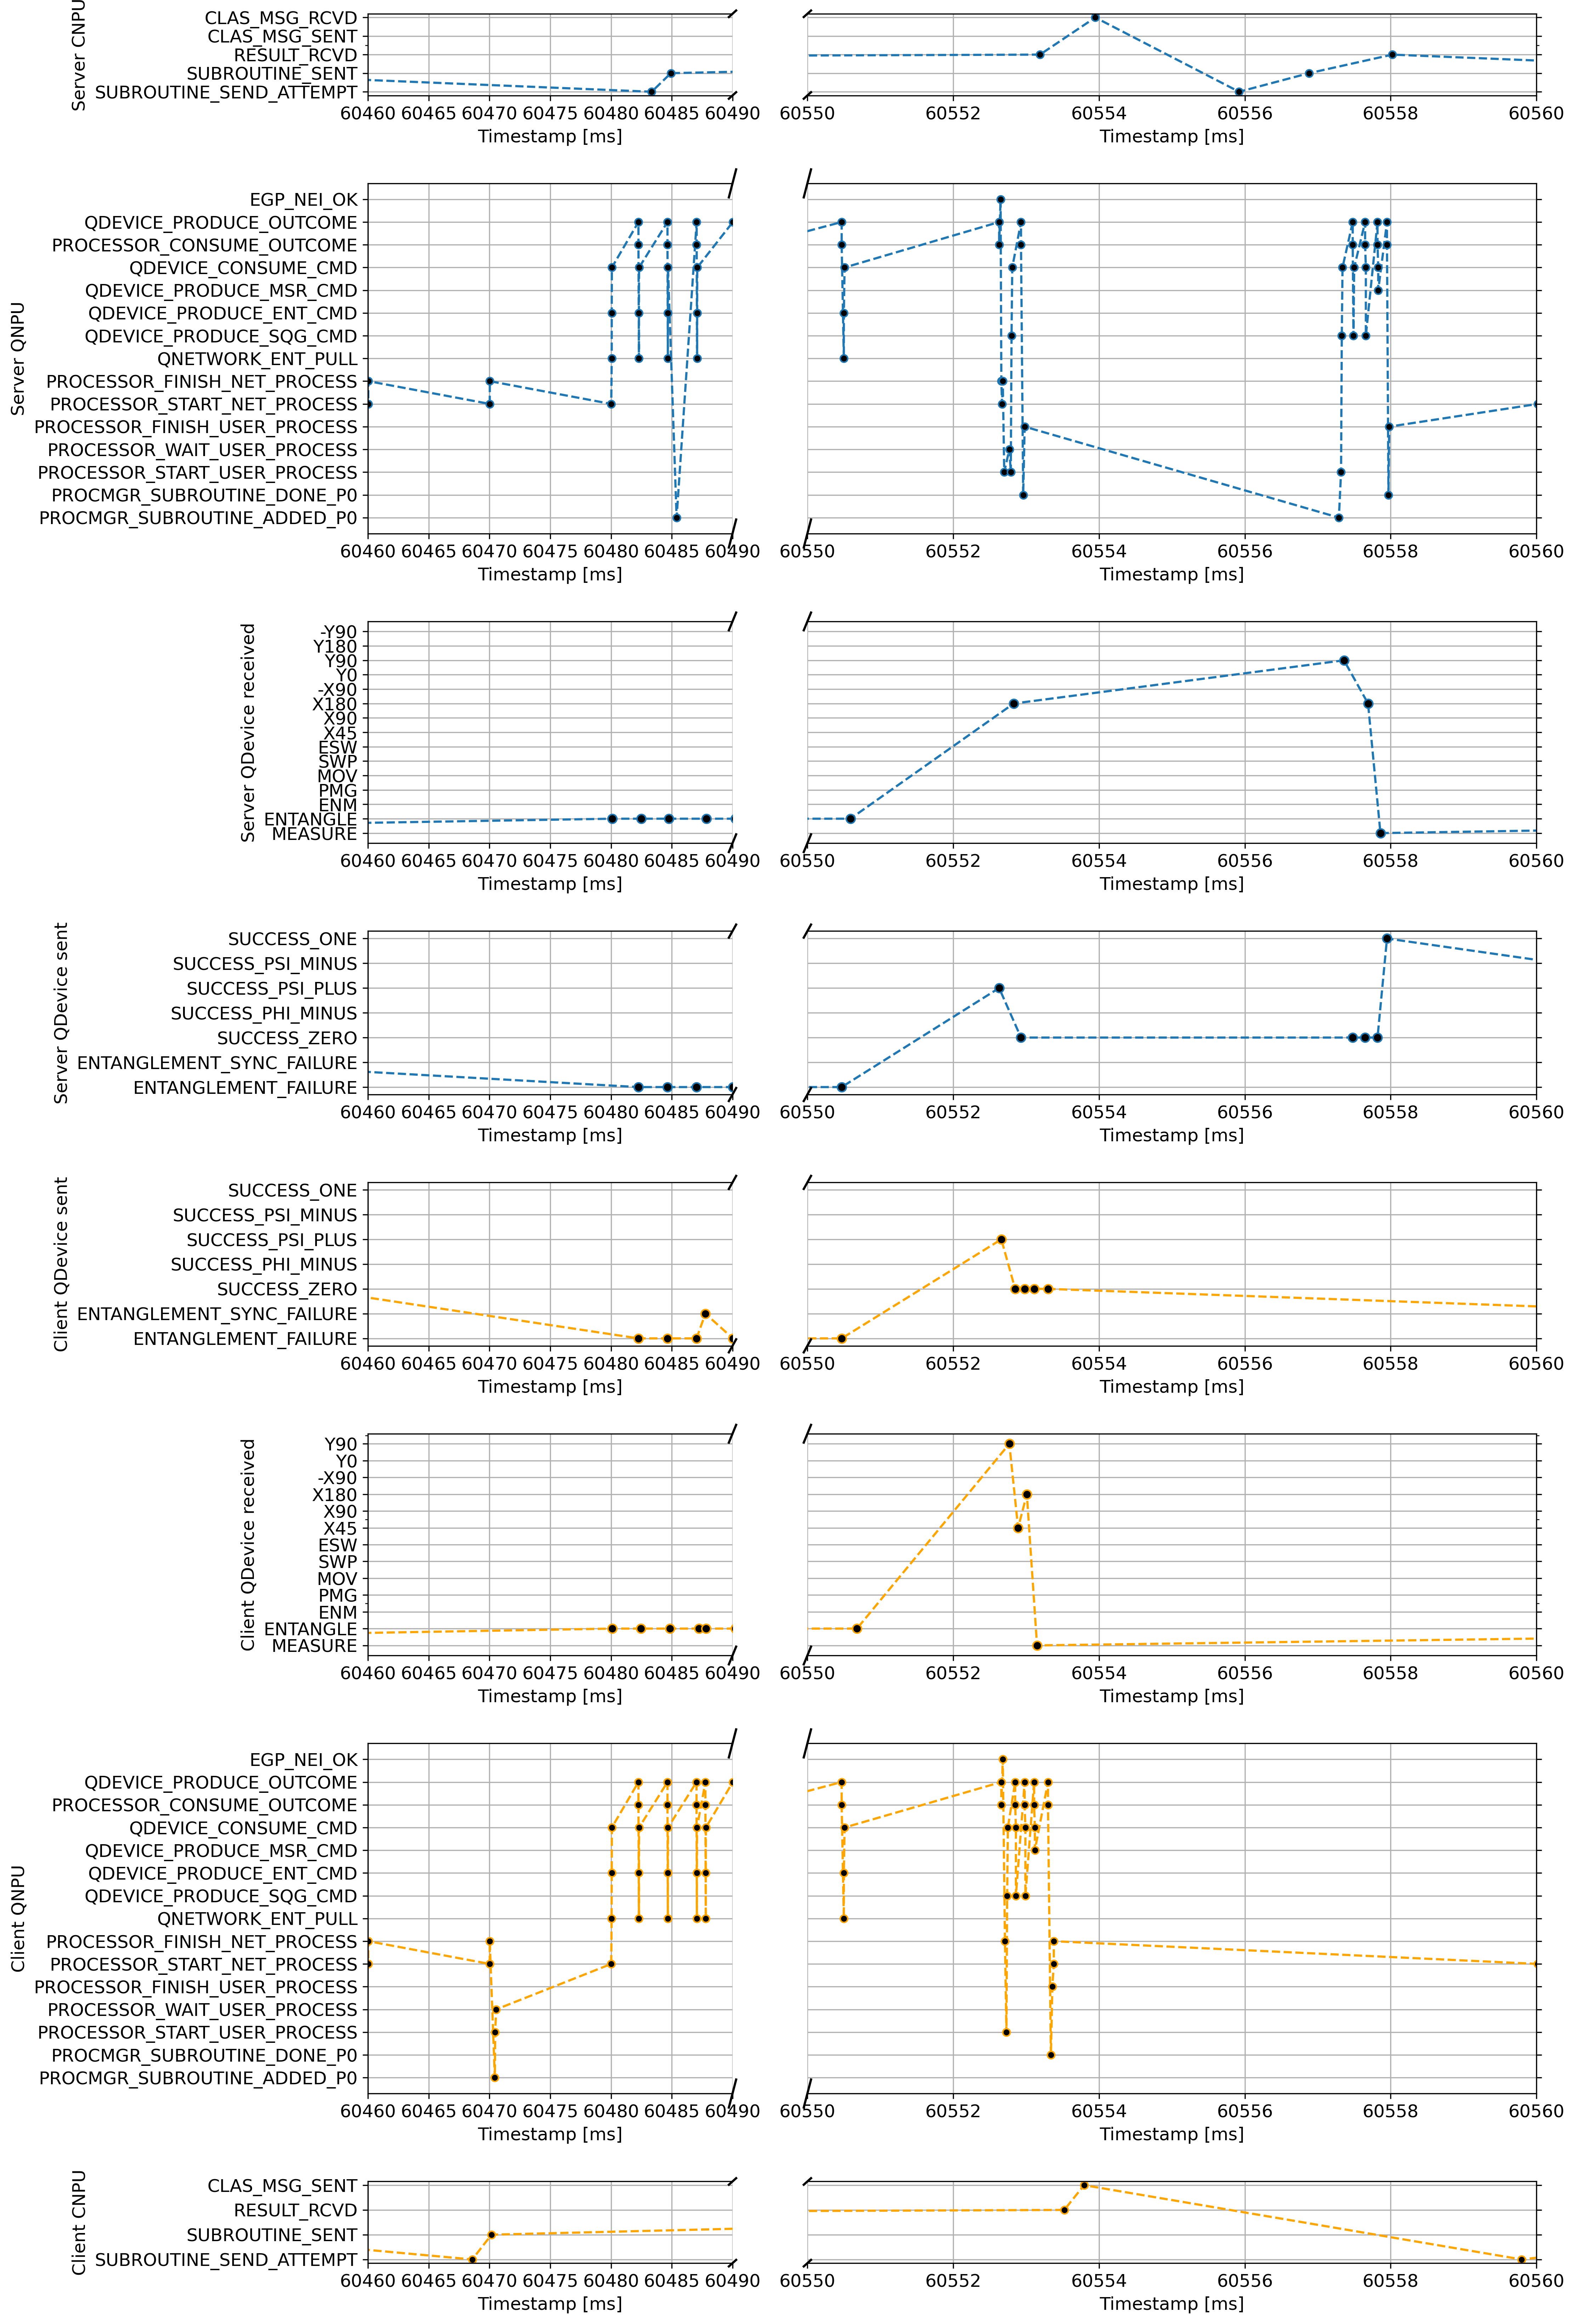
\includegraphics[width=1.0\textwidth]{figures/qnodeos/supplementary/plots/full_slice.png}
\caption{Full-stack event trace for one particular execution of the \ac{DQC} circuit. Between timestamps 60490 and 60550 are more entanglement attempts which are cut out for the sake of clarity.}
\label{qnodeos:fig:delcomp-trace-example}
\end{figure*}


\begin{xstretch}
\printbibliography[heading=subbibintoc,title={References},notcategory=noprint]
\end{xstretch}
\chapter
 [Qoala: an Application Execution Environment for Quantum Internet Nodes]
 {Qoala: an Application Execution Environment for Quantum Internet Nodes}
\label{chp:qoala}

\begin{abstract}
Executing quantum internet applications presents unique challenges not encountered in quantum computing.
These challenges include the need for a highly interactive execution of hybrid classical-quantum programs running at different network nodes, where the limited lifetime of quantum memories imposes deadlines to achieve a desired level of performance. What's more, part of the execution is subject to strict timing constraints (e.g. entanglement generation), while others allow more flexible timing precision (e.g. classical messages exchanged between the nodes). 
Here, we present Qoala, the first execution environment for programmable nodes in a quantum internet to address these challenges including:
(1) A unified program format for hybrid interactive classical-quantum programs, providing a well-defined target for compilers, and 
(2) A runtime representation of a program that allows joint scheduling of the hybrid classical-quantum program, multitasking, and asynchronous program execution.
Based on concrete design considerations, we put forward the architecture of Qoala, including the program structure and execution mechanism.
We implement Qoala in the form of a modular and extendible simulator that is validated against real-world quantum network hardware (available online).
However, Qoala is not meant to be purely a simulator, and implementation is planned on real hardware.
We evaluate Qoala's effectiveness and performance sensitivity to latencies and network schedules using an extensive simulation study.
Qoala provides a framework that opens the door for future computer science research into quantum network applications, including scheduling algorithms and compilation strategies that can now readily be explored using the framework and tools provided. 
\end{abstract}

\iffullchapters
\section{Introduction}
\label{qoala:sec:introduction}

\begin{figure}% [ht]
    \centering
    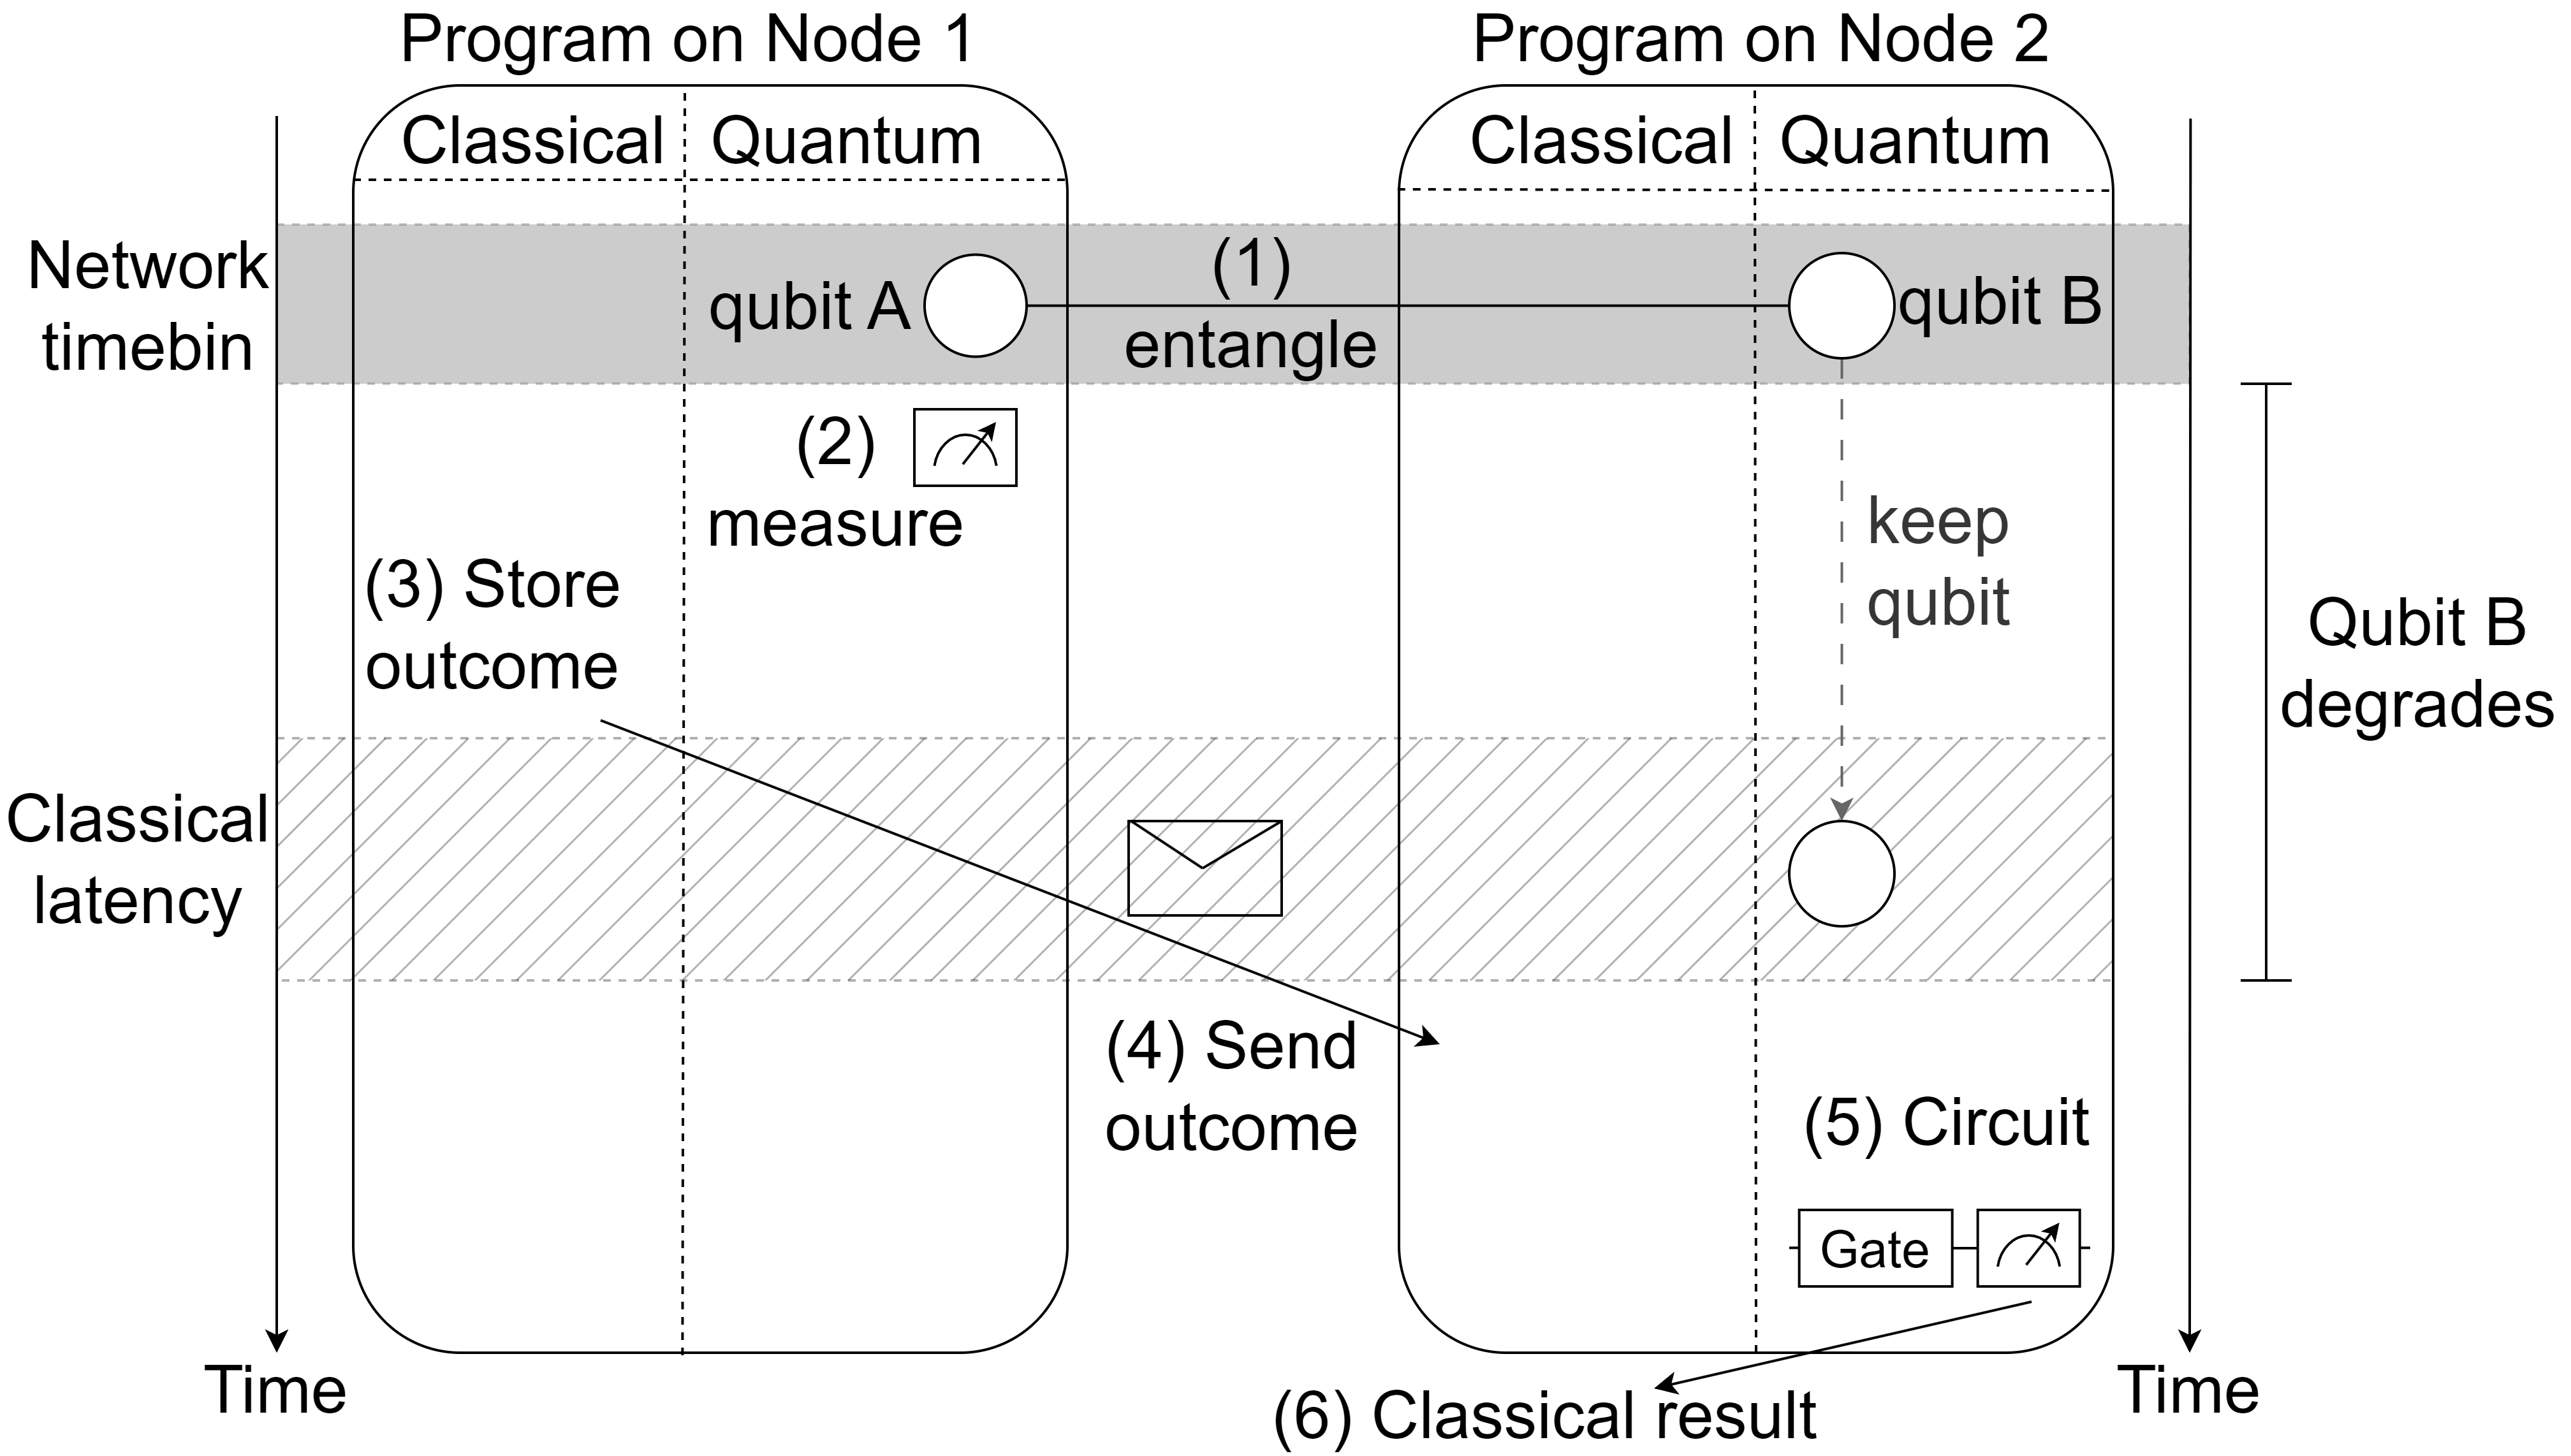
\includegraphics[scale=0.35]{figures/qoala/program_illustration.png}
    \caption{Example application consisting of two hybrid classical-quantum programs (on Nodes 1 and 2) including
        (1) Entanglement generation between two qubits (circles) in a synchronized time slot (defined by  network controller).
        (2) A local measurement of qubit A at Node 1 resulting in a classical outcome bit (destroying the qubit)
        (4) Communication of the classical bit from Node 1 to Node 2 (taking non-deterministic time)
        (5) Execution of a quantum circuit on qubit B at Node 2 depending on the classical bit. The quality of qubit B has degraded during the time elapsed since (1). 
        (6) Node 2 measures qubit B and outputs the classical result.
    }
    \label{fig:program_illustration}
\end{figure}


Advances in quantum computing and quantum communication technologies are paving the way for a \textit{quantum internet}~\cite{wehner2018quantum, kimble2008quantum}, where quantum applications are executed across multiple network nodes.
Examples of such applications include quantum key distribution (QKD)~\cite{bennett2014quantum, ekert1991quantum} and blind quantum computation (BQC) \cite{broadbent2009universal, arrighi2006blind} from a client to a quantum cloud server.
A multi-node quantum internet application is partitioned into separate single-node \textit{programs} (e.g. a client program and a server program in BQC) that run concurrently on different network nodes. To support security sensitive applications, each program performs local classical and quantum computations on its own private node, and programs interact with each other only via classical message passing and entanglement generation. This is in sharp contrast to distributed quantum computing (see e.g.~\cite{cacciapuoti2019quantum}), where all nodes can be accessed and controlled by a single program. 

The single-node programs that constitute a quantum internet application are hybrid in nature (see Fig~\ref{fig:program_illustration}):
First, they contain quantum operations, such as local quantum gates and measurements (e.g. to perform a server computation in BQC), and entanglement generation (e.g. to produce key in QKD). Entanglement is a special property of two quantum bits (qubits) that forms a key resource for quantum internet applications. 
All quantum operations are executed on quantum processors that can store, manipulate and measure quantum information, where small networks including such processors have been realized using different quantum hardware platforms including, for example,  Nitrogen-Vacancy (NV) centers in diamond~\cite{pompili2021realization}, and Ion Traps~\cite{krutyanskiy2023entanglement}.
Second, programs need to perform classical operations, such as message passing (e.g., a BQC client program sending desired measurement bases to the BQC server), and local classical processing (e.g., post-processing measurement outcomes in QKD).

Realizing the execution of quantum internet applications presents unique challenges (see Section~\ref{qoala:sec:design_considerations}): 
First, a program for a quantum internet application is not merely a hybrid of classical and quantum code segments; these segments are also highly \textit{interactive}: classical and quantum code may run concurrently, communicating and influencing each other.
E.g., a quantum circuit may "pause" halfway, keeping quantum states in memory, and wait for a value from a classical segment (e.g. a classical message from a remote node) before continuing.
Quantum memories have limited lifetimes, meaning qubits are subject to decoherence, degrading their quality over time. This introduces the need 
control the joint schedule of the classical and quantum segments of the program to reach desired levels of application performance.

Second, a compiler should be able to optimize the whole program including both classical and quantum code, as well as to provide information that can be used in our architecture to align and inform scheduling decisions. 

Finally, we are faced with a mix of time scales:
on the one hand, entanglement generation requires a very precise network schedule that is agreed ahead of time between the network nodes~\cite{dahlberg2019link}. On the other hand, classical messages are exchanged asynchronously between the nodes without guaranteed message delivery times. This motivates an architecture in which different segments of the system may operate at different levels of timing precision. 

\subsection{Main contributions}
We propose the first architecture, Qoala, that addresses these challenges. Qoala is an execution environment tailored to programmable quantum internet nodes, accommodating the \textbf{hybrid, interactive, networked, and asynchronous nature} of quantum internet applications. 

\textbf{Unified program format for hybrid-classical quantum programs:}
Qoala defines a unified program format for executables, encompassing classical and quantum (networked and local) code, and defining basic blocks.
This paves the way for a joint optimization of the classical and quantum code by a compiler.
% The program format is also made such that it can be the output of a compiler, making use of basic blocks.

\textbf{Runtime representation allowing scheduling:} Qoala separates the static unified program format from a runtime representation consisting of \textit{tasks}. 
This paves the way to design and implement algorithms for scheduling the quantum program in order to meet deadlines imposed by decoherence of the quantum memory.  
To provide advice to the scheduler on deadlines to achieve a desired program performance, programs can specify advice for timing and prioritization depending 
on the quantum hardware capabilities of the node. 
The separation of a static program from its runtime tasks also allows for the programmer to define asynchronous code segments, the execution of which is decided by the scheduler alone.
This is the first architecture that allows for effective scheduling control of hybrid interactive classical-quantum programs, thus addressing a critical issues in the successful execution of quantum internet applications.

\textbf{Integration with quantum network stack:}
Qoala integrates with an existing quantum network stack~\cite{dahlberg2019link} implemented on NV centers in diamond~\cite{pompili2022experimental} for realizing entanglement generation between nodes. This opens the door for Qoala to be implemented on such networks.

\textbf{Implementation in hardware validated simulation:} We implement the proposed architecture as a \textbf{modular and composable simulator}, which enables the evaluation of different execution strategies and techniques.
The simulation is validated against real-world quantum hardware implementations, opening the door to understand performance tradeoffs and requirements for Qoala's implementation. Specifically, the simulator allows 
configuring different hardware parameters, latencies, and software component organizations, to evaluate implementation choices of Qoala in simulation. 

Using the implementation we demonstrate the effectiveness and feasibility of our proposed architecture on different types of quantum hardware, including its ability to schedule and multitask applications using a number of existing scheduling methods (EDF, FCFS).
We continue to examine tradeoffs in the classical and quantum performance metrics of using different types of scheduling approaches. 
We examine Qoala's improvement over NetQASM~\cite{dahlberg2022netqasm} in enabling hybrid classical-quantum compilation possibilities. 
Finally, we study trends in application performance when varying the amount of concurrency, and examine the impact of a network schedule for entanglement generation on the performance of Qoala.

We highlight the role of Qoala in opening the door for computer science research. We make our simulator available as open source~\cite{qoala2023simulator}, paving the way for computer scientists to conduct further research, e.g., into the design of compilers, or schedulers that can readily be tested using the simulator. 

The remainder of this paper is structured as follows. Section~\ref{qoala:sec:related_work} compares our work to related studies. In Section~\ref{qoala:sec:design_considerations} we explain important context and terminology, followed by considerations that we used to design our architecture (Section~\ref{qoala:sec:architecture}). Section~\ref{qoala:sec:implementation} discusses our implementation and Section~\ref{qoala:sec:evaluation} provides evaluation results using this implementation. We conclude and give suggestions on future work (Section~\ref{qoala:sec:conclusion}).


\section{Related work}
\label{qoala:sec:related_work}

Networks of quantum processors have been realized using different quantum hardware platforms including, for example, nitrogen-vacancy (NV) centers in diamond~\cite{pompili2021realization}, and trapped ions~\cite{krutyanskiy2023entanglement}.
A first operating system QNodeOS~\cite{donne2024design} (see also \cref{chp:qnodeos}) including a network stack~\cite{pompili2022experimental} has been designed and implemented on real quantum network nodes based on NV centers in diamond.
QNodeOS makes use of the NetQASM execution framework~\cite{dahlberg2022netqasm} (see also \cref{chp:netqasm}), where a classical network processing unit (CNPU) dispatches NetQASM routines for execution by a quantum network processing unit (QNPU).
This meant, e.g., that QNodeOS was unable to have any scheduling control over the joint classical-quantum execution, which could lead to a failure in executing programs successfully.
Our work builds on top of ideas of QNodeOS and NetQASM, but addresses critical challenges that were not handled by these previous systems, including the ability to schedule hybrid programs and to optimize over the whole program code (see \cref{qoala:fig:qoala_vs_qnos} for a comparison).
Building on the only such systems that have seen real world implementation on quantum hardware, opens the door for a later implementation of Qoala on quantum hardware by implementing an improved low-level classical control hardware architecture (\cref{qoala:sec:architecture}).

\begin{figure}[t]
    \centering
    \includegraphics[width=0.7\textwidth]{figures/qoala/qoala_vs_qnos.pdf}
    \caption{
        QNodeOS (\cref{chp:qnodeos}) vs. Qoala capabilities.
    }
    \label{qoala:fig:qoala_vs_qnos}
\end{figure}

Research has been done on related topics, such as distributed quantum computing, or hybrid (non-interactive) quantum computing. Hybrid classical-quantum programs have been extensively studied in quantum computing, e.g. in the context of \textit{variational quantum eigensolvers (VQE)}~\cite{diadamo2021distributed, liu2022layer} or \textit{quantum approximate optimization algorithms (QAOA)}~\cite{farhi2014quantum}. However, they differ in two important aspects: although they are hybrid, they are not \textit{interactive} during the quantum execution:
(1) classical and quantum segments do not run concurrently, but quantum segments are executed in their entirety before returning to classical segments, i.e. no quantum state is kept in the processor between the execution of different quantum segments.
(2) such hybrid programs lack network interoperability (entanglement generation and classical message-passing between nodes), and also do not have the same timing and flexibility requirements.

Distributed quantum computing~\cite{cacciapuoti2019quantum} shares similarities with quantum internet applications but differs in several aspects.
In the former, complete control is assumed over all participating nodes, such as an application distributed across multiple cores on a single chip~\cite{ovide2023mapping, jnane2022multicore}.
Generally, the capabilities of each core and the latencies between them are fully known, allowing for precise scheduling and orchestration of individual programs running on each core to optimize overall execution.
In contrast, programs in quantum internet applications operate independently (and may even be running on different quantum hardware); therefore they have a degree of autonomy in their own scheduling, and are not fully aware of the actions or timing of other programs.

Entanglement distribution in networks is another related topic that has been extensively studied (see e.g. surveys~\cite{wei2022towards, azuma2021tools}).
However, these works do not deal with executing network applications, and give only predictions for applications in which entanglement is immediately measured (e.g. QKD).

The concept of (soft) deadlines for program execution is of course well known from classical real-time systems that are often used in domains where deterministic and time-critical response is essential, such as automotive, aerospace and medical devices~\cite{liu1973scheduling, hambarde2014survey, buttazzo2011hard}, including examples of systems with mixed timing precision~\cite{burns2017survey}.
We draw inspiration from this domain, and the present architecture opens the door to explore algorithms and concepts from this domain to be applied to the execution of quantum internet applications.

\section{Design considerations}
\label{qoala:sec:design_considerations}

\subsection{Background and context}
\label{qoala:sec:background_context}

We first revisit some of the relevant background and context (see also \cref{chp:background}).

\textit{Quantum nodes}.
A quantum internet connects quantum nodes on which quantum programs may be 
executed.
%(\cref{qoala:fig:qoala_location}). 
In their most general form, such nodes
are \textit{processing nodes} that have a quantum memory to store quantum bits (qubits) on which quantum operations (qubit initialization, quantum gates and measurements) can be performed. Pairs of nodes can establish \textit{entanglement} between them over a quantum network. Entanglement is a special property of two qubits (an \emph{entangled pair}), where one qubit is stored in the memory of each node. Nodes can also exchange classical messages (e.g. via dedicated classical links or the internet), where no guarantees are assumed on their message delivery times. 

\textit{Programs}.
A program is a series of instructions to be executed by a node.
Instructions can be categorized into four types: local classical processing, classical message-passing, quantum local processing (quantum operations), and remote entanglement generation.
A program can keep classical variables in a classical memory, and quantum variables (qubits) in the node's quantum memory during the execution.
Multiple programs, each running on their own node, together form an \textit{application} (see \cref{qoala:fig:program_illustration}), e.g. QKD (two programs, one per node),
or secret sharing~\cite{hillery1999quantum} (a program each on many nodes).
Programs may involve asynchronous operations (e.g. a server awaiting entanglement with multiple clients).

\textit{Network schedule}.
A quantum network stack has been proposed~\cite{dahlberg2019link} and implemented \cite{pompili2022experimental} that turns entanglement generation into a robust service independent of the quantum hardware platform.
Important for the design of an architecture for the execution of quantum internet applications is that in this stack, the nodes will establish a network schedule of time slots in which they will trigger entanglement generation (due to need to synchronize entanglement generation at the physical layer~\cite{dahlberg2019link} at nanosecond precision).
This means that once entanglement has been requested from the network, the nodes can use only the slots in the network schedule to produce entanglement between them, imposing constraints on the ability to schedule applications. What's more, in present day systems~\cite{pompili2021realization, krutyanskiy2023entanglement} limitations in the physical devices prohibit the execution of local operations while engaging in network operations (entanglement generation), creating further dependencies between the local quantum execution and entanglement generation. 
As the specifics of network scheduling~\cite{network-scheduling, skrzypczyk2021architecture} are not within scope of this thesis,
we assume the existence of a \textit{network controller} that takes application demand for entanglement and issues a network schedule to the nodes. 
A schedule consists of sequential time slots, each with a start time and duration, when the node will trigger entanglement generation.
Nodes are not forced to attempt entanglement in corresponding time slots, and can instead choose to do local processing instead.


\textit{Performance metrics and noise}. Quantum internet applications have classical outcomes that are typically probabilistic in nature:
(1) applications may intentionally do measurements on quantum states that have fundamentally probabilistic outcomes (e.g. quantum cryptography),
(2) in practice, quantum hardware is imperfect (or \textit{noisy}). That is, undesired errors occur
when performing operations (such as gates, measurements, or entanglement generation) or when keeping quantum states in memory for too long.

In many quantum internet applications (e.g. BQC), a single execution of the application can result in failure or success (e.g. a BQC client receives correct measurement results from the server program~\cite{leichtle2021verifying}). Applications are often executed many times, where outcome statistics are computed in order to validate successful execution (e.g. by majority of outcomes).
We consider two metrics:
a \emph{quantum metric} --- the \textit{success probability} of executing a single instance of the application (on average), and a \emph{classical metric} --- the \textit{makespan}, i.e. the average execution time of an application instance.

\subsection{Considerations}
Considerations can be categorized into three main groups: fundamental, technological, and enabling.

\noindent\textit{\textbf{Fundamental Considerations}}
(1) \textit{Hybrid nature of applications (FC1)}: Quantum internet applications inherently consist of both classical and quantum segments, as well as local and networking operations. The execution environment must account for this hybrid nature, and the program structure should accommodate all types of operations.
(2) \textit{Interactive nature of applications (FC2)}: Quantum internet applications require classical communication between nodes. This communication may take place in between classical and quantum segments of a single program. 
This implies the need for application-level interfaces between programs on different nodes, and for interfaces between classical and quantum code segments on a single node.
(3) \textit{Multitasking (FC3)}: Programs may spend a significant amount of time waiting for messages from a remote node (ms), motivating multitasking to make optimal use of the classical and quantum computing resources at each node.  This requires scheduling of time and resources.

\noindent\textit{\textbf{Technological Considerations}}
(1) \textit{Limited qubit lifetime (TC1)}:
Quantum memory quality degrades over time, presenting a significant challenge for the execution environment,
especially in near-term hardware (ms to s memory lifetimes~\cite{ruf2021quantum, pompili2021realization, krutyanskiy2023telecom}).
As such, there are natural deadlines to application execution after which a desired performance (success probability) can no longer be reached.
We thus desire that a program specification allows indication of memory quality constraints (deadlines), which the runtime environment can act upon (e.g. by appropriate scheduling or restarting).
(2) \textit{Integration of processing and networking (TC2)}: We assume that near-term nodes only have a single quantum processor, which needs to perform both local quantum gates as well as remote entanglement generation.
That is, while performing local operations the processor is blocked from networking operations and vice versa, as is the case for all current implementations~\cite{pompili2021realization, krutyanskiy2023entanglement} but may be mitigated partially using future proposals~\cite{vardoyan2022quantum}. 
The node must hence allocate time for local computation while at the same time adhering to the network schedule which constrains timing of the entanglement operations.

\noindent\textit{\textbf{Enabling Considerations}}
(1) \textit{Different compilation strategies and programming languages (EC1)}: The execution environment should support various compilation strategies and accessible programming languages. 
In order to enable compilation, we furthermore want a representation of the program that can be integrated with existing compiler frameworks.
(2) \textit{Different scheduling strategies (EC2)}: Since we expect that scheduling plays a vital role in optimizing application performance, the execution environment should enable scheduling, and support different scheduling algorithms and policies, 
allowing for their comparison and evaluation.
(3) \textit{Different (control) hardware implementations (EC3)}: The architecture should make minimal assumptions on the classical control hardware, and be independent on the choice of quantum hardware platform~\cite{carlothesis},
allowing for integration with multiple (future) technologies such as NV centers~\cite{pompili2022experimental} or trapped ions~\cite{drmota2023robust}.


\section{Architecture}
\label{qoala:sec:architecture}

Based on these design considerations, we propose Qoala (see Fig.~\ref{fig:runtime_overview}), an execution environment for programmable nodes in a quantum internet. 
Provided minimal hardware assumptions are met (Section~\ref{qoala:sec:minimal_hardware_assumptions}), 
each node implements its own Qoala execution environment, supporting a specific \textit{program structure} (Section~\ref{qoala:sec:program_structure})
and implementing a specific \textit{runtime environment} (Section~\ref{qoala:sec:runtime_environment}) that is able to \textit{schedule tasks} (Sections~\ref{qoala:sec:tasks}--\ref{qoala:sec:scheduling}).
Details in Appendices~\ref{qoala:sec:app:program_structure}, \ref{qoala:sec:app:runtime_environment}, \ref{qoala:sec:app:scheduling_execution}.

\subsection{Minimal hardware assumptions}
\label{qoala:sec:minimal_hardware_assumptions}

Qoala is based on only a few core assumptions on the processing node (Figure~\ref{fig:minimal_hardware_assumptions}):

\textit{CPS-QPS distinction}. We assume the node distinguishes between a \textit{classical processing system (CPS)} managing classical computing resources (e.g. CPU, classical memory and networking), and a \textit{quantum processing system (QPS)}, responsible for executing quantum operations (gates, measurements, entanglement generation) on quantum hardware including a quantum memory as in~\cite{dahlberg2022netqasm, pompili2022experimental}.
Unlike prior work, we assume a shared classical memory is accessible to both the CPS and QPS, enabling communication between the two processing systems, addressing the interactive property of quantum internet programs.
The CPS can act as a fully-fledged classical computer, and performs application-level classical communication with other nodes as well as with a network controller who sets a network schedule.
The QPS can execute routines consisting of low-level quantum gates, basic classical control logic (branching), and entanglement generation.
This opens the door for the QPS to be based on essentially any quantum hardware platform where a specialized microcontroller is used to control the quantum hardware, and a separate microprocessor implements the CPS, where a shared memory could be realized next to the two processors on-chip.
The scheduler controls both CPS and QPS execution, and may physically be realized on either one.

\textit{Time granularity}. Both CPS and QPS are assumed to have knowledge of time, albeit operating with different timing precision ($ms$ precision for CPS mirroring node-to-node communication latencies vs. $\mu s$ and $ns$ precision needed for synchronized entanglement generation~\cite{pompili2022experimental, dahlberg2019link}.)

 \textit{Network stack}. A quantum network stack including a network layer~\cite{dahlberg2019link} is implemented on the node with which Qoala can interface. This stack can receive and fulfill requests for remote entanglement generation.
\begin{figure}
    \centering
    \includegraphics[width=\columnwidth]{figures/qoala/minimal-hardware.png}
    \caption{Minimal hardware assumptions for a single node.}
    \label{fig:minimal_hardware_assumptions}
\end{figure}



\subsection{Program structure}
\label{qoala:sec:program_structure}
Qoala defines a hybrid format for programs, addressing considerations in Section~\ref{qoala:sec:design_considerations}.
A Qoala program is a combination of quantum and classical instructions, 
organized into three main sections: \textit{host code} (containing classical instructions), \textit{local routines} (containing local quantum instructions), 
and \textit{request routines} (for remote entanglement generation).
This hybrid format allows a compiler to optimize the whole program, including critical code paths with dependencies between classical and quantum segments.
Local routines and request routines can be triggered from within host code as function calls, addressing the interactivity between them.

A Qoala program is an \textit{executable} and output of a compiler.
The format is separate from any high-level language in which a programmer might write code; hence Qoala in theory allows for compatibility with any such language.
Entry and exit points of a program are in host code.
Figure~\ref{fig:example_program} shows an example program in text format.
We contrast Qoala's program format with that of~\cite{dahlberg2022netqasm}, in which there was no way to compile across classical and quantum code segments.
A Qoala program has \textit{program arguments} that are filled in during program instantiation (Section~\ref{qoala:sec:program_instantiation}).


\begin{figure}%[ht]
    \centering
    \includegraphics[width=\columnwidth]{figures/qoala/runtime_overview.png}
    \caption{High-level overview Qoala: An SDK allows program code in a high-level language (e.g. Python).
    A compiler translates this code into a Qoala program (specific compiler not in scope of this work).
    To run, a program is instantiated with concrete values for program arguments.
    Tasks are created for the program instance, which are scheduled and executed by the scheduler.
    Multiple program instances may exist at the same time (both multiple instances of the same or different programs).
    All tasks from all instances are added to a single task graph (Section~\ref{qoala:sec:tasks}) used by the scheduler.
    }
    \label{fig:runtime_overview}
\end{figure}




\textit{Host code}.
Host code, executed on the CPS, encompasses local computation, control-flow, inter-node messaging, and can initiate local and request routines.
For example, in a program that is part of a QKD application, classical post-processing (including sending bases, local error correction, and privacy amplification \cite{vidick2023introduction}) would be represented in host code.
Host code is structured as a sequence of \textit{blocks}, each holding a list of instructions.
Blocks dictate control-flow by ending with a (conditional) jump instruction (default: next block in the sequence).
This block division not only facilitates task creation and scheduling (see Section~\ref{qoala:sec:tasks}) but also streamlines compiler integration (which may use blocks in its intermediate representation).
Blocks can contain metadata about their expected \textit{duration}, (relative) deadlines, and they may be inside \textit{critical sections}, encompassing a sequence of blocks with a maximally allowed execution duration. This metadata is propagated to corresponding tasks and used by the scheduler in order to mitigate quantum decoherence due to limit qubit lifetime.
Asynchronous execution is possible by `submitting' multiple routines for execution, and waiting for all of them to finish. At runtime, the scheduler can decide in which order to execute the routines.


\textit{Local routine}.
A local routine (LR) represents a series of quantum operations (like gates and measurement), to be executed by the QPS locally (no interaction with external nodes or controllers).
An LR may also contain limited classical computation and control-flow code allowing for fast feedback, which can increase quantum performance (Section~\ref{qoala:sec:background_context}) due to less decoherence.
An updated version of NetQASM~\cite{dahlberg2022netqasm} is used to represent the instructions, which allows both hardware-specific and hardware-agnostic instructions.
Therefore, the program format is compatible with different quantum hardware.
In contrast to \cite{dahlberg2022netqasm}, Qoala's version of NetQASM does not have instructions for entanglement generation (cleanly separating local and networked quantum operations)
nor `wait' instructions. This allows routines to be treated as atomic non-preemptable blocks.
%, which makes scheduling easier).

\textit{Request routine}. A request routine (RR) consists of a request for entanglement generation with another node, and represent requests to the node's quantum network stack.
It can have local routines as callbacks, allowing quick local (quantum) processing of entangled qubits on the QPS without returning to the CPS, decreasing waiting time and decoherence.


\subsection{Runtime environment}
\label{qoala:sec:runtime_environment}
The Qoala runtime environment provides various resources that programs can leverage during execution.

\textit{Exposed Hardware Interface (EHI)}.
The Exposed Hardware Interface provides information about the hardware and software capabilities and restrictions of the node and the network,
like available quantum memory and expected latencies.
Each node provides their own EHI which is used in capability negotiation (see below), and allows a choice of executable code optimized by a compiler for those capabilities ahead of time. 

\textit{Shared memory}.
To address the classical-quantum interactivity in programs, the CPS and QPS share data with each other via \textit{shared classical memory}.
Write conflicts are avoided by explicit read/write rules for shared memory regions.
Our conceptual model of a shared memory leaves open different implementation choices, including a physical shared memory or a message-passing protocol.
Calls in host code to local or request routines use the shared memory to communicate routine arguments and results.

\textit{Quantum memory}.
Quantum memory is organized into a \textit{virtual quantum memory space (VQMS)} for each program instance (see Section~\ref{qoala:sec:program_instantiation} for instantiation), represented as Unit Modules~\cite{dahlberg2022netqasm}.
Qoala maps each VQMS to the physical qubits available in the QPS.
VQMS information like qubit connectivity and noise characteristics is provided by the EHI, which a compiler can use to optimize a program.
The VQMS enables multitasking since programs have their own runtime context, while a scheduler (Section~\ref{qoala:sec:scheduling}) sees the whole physical memory space and can schedule programs accordingly.

\textit{Remote interaction}. For interaction with programs on remote nodes,
the runtime provides \textit{classical sockets} and \textit{EPR sockets} based on~\cite{dahlberg2022netqasm}. Host code uses classical sockets for sending and receiving messages; EPR sockets are indicated in request routines (see e.g. Figure~\ref{fig:example_program}).

\begin{figure}% [ht]
    \centering
    \includegraphics[width=\columnwidth]{figures/qoala/example_program.png}
    \caption{
        Example Qoala program containing a host section with 4 blocks, a local routine (\texttt{subrt1}),
        and a request routine (\texttt{req1}). Block \texttt{b2} has a relative deadline to \texttt{b0} of $0.1$ times qubit noise parameter $T_2$.
    }
    \label{fig:example_program}
\end{figure}

\begin{figure*}
    \newcommand{\figheight}{6.5cm}
    \centering
    \subfloat[\centering \label{fig:task_types}]{{\includegraphics[height=\figheight, keepaspectratio]{figures/qoala/task-types-table.png}}}%
    \hfill
    \subfloat[\centering \label{fig:task_creation_cutout}]{{\includegraphics[height=\figheight, keepaspectratio]{figures/qoala/task_creation_cutout.png}}}%
    \caption{
        (a) Overview of task types.
        (b) Examples of host code and corresponding task graphs.
        Shaded tasks are executed by the QPS, the others by CPS.
        Top: asynchronous submission of local routines \texttt{s1} and \texttt{s2}.
        The graph consists of two separate chains of tasks and the scheduler can choose in which order to execute these chains (possibly interleaved).
        Bottom: a request routine uses the callback entry to immediately add tasks for executing local routine \texttt{cb} after each entangled pair generation.
    }%
    \label{fig:tasks}
\end{figure*}

\subsection{Tasks}
\label{qoala:sec:tasks}
We introduce \textit{tasks} to enable multitasking.
Each task represents a code segment of a running program with a context of runtime variables.
Tasks have different types (Figure~\ref{fig:tasks}) based on the code they represent.
By splitting a program into distinct executable tasks, 
we can utilize the parallel execution on the CPS and QPS (by assigning tasks to the corresponding system),
and we can interleave execution of multiple programs by filling waiting times of one program by execution of tasks of another.
Code segments indicated to run asynchronously (Section~\ref{qoala:sec:program_structure}) can also be represented by tasks, the execution order of which can then be governed by a scheduler.
%, simplifying the interface between the developer's intent (`run these segments in any order') and the runtime system (choosing an efficient execution order).
Further, tasks enable interleaving of local operations and quantum network (entanglement generation) operations.
A scheduler can choose when to execute entanglement tasks (with strict timing requirements from the network schedule)
and when to execute local tasks (less strict requirements).

\textit{Task graph}.
Tasks are organized in a \textit{task graph}, a directed acyclic graph (DAG) where each node represents a single task.
Edges can be \textit{precedence constraints} (task A must conclude before task B initiates) or \textit{relative deadlines} (task B should start within maximum duration $t$ after completion of task A).
Using a task graph introduces a well-defined and isolated scheduling problem: given a graph of tasks, which task(s) should be executed next?
Deadlines are used to assist the scheduler (see below) in mitigating the gradual quality degradation of quantum states over time (decoherence) by choosing appropriate tasks.
Some tasks are only enabled after certain events happen.
\texttt{HostEvent} tasks are enabled by an incoming classical message and \texttt{SinglePair} or \texttt{MultiPair} tasks are enabled by network schedule timestamps.
Tasks also have information about what quantum memory they use, helping the scheduler decide which tasks it can execute at a given time.

\textit{Task creation}. 
A task is created for a segment of a running program.
If a program segment is executed multiple times (e.g. because of a loop in the code), this results in multiple tasks.
A host code block is translated into a \texttt{HostLocal} task (block contains only local instructions) or a \texttt{HostEvent} task (block starts with a `receive message' instruction).
A local routine call is represented by (1) a \texttt{PreCall} task (CPS allocates shared memory and writes routine arguments), (2) a \texttt{LocalRoutine} task (QPS executes routine), and (3) a \texttt{PostCall} task (CPS reads routine results from shared memory).
Request routine calls are handled similarly (with \texttt{SinglePair} or \texttt{MultiPair}).
\texttt{MultiPair} tasks can be more time- and resource efficient since the network stack can handle multiple pair generations at once.
Callback tasks for local routines acting as entanglement generation callbacks allow quick successive execution.
For each task, its expected duration is calculated based on the metadata of the corresponding block or routine in the program, together with information from the EHI (see below).
See Figure~\ref{fig:task_types} for task types and Figure~\ref{fig:task_creation_cutout} for examples of host code and corresponding tasks (details in Appendix~\ref{qoala:sec:app:scheduling_execution}).


\subsection{Program instantiation}
\label{qoala:sec:program_instantiation}
A program is part of an application that uses entanglement generation orchestrated by a network controller (Figure~\ref{fig:program_illustration}).
Therefore, before execution, the program must align with the other programs of its application as well as with the network controller.
(1) \textit{Capability negotiation and entanglement demand registration}.
First, all collaborating nodes exchange their EHI and agree on concrete values for deadlines and task duration estimations (using advice pre-computed by the compiler).
These values are needed to do effective scheduling at runtime.
Second, the nodes together register their entanglement demands to the network controller, which then creates a \textit{network schedule} based on these.
This schedule consists of time slots, each of which is assigned to an individual \textit{application instance} (tuple of program instances, one per node).
(2) \textit{Program instantiation}. Concrete values for program arguments can be filled in such as deadlines, durations and program-specific input values.
Typically, for a given application, the involved nodes create many \textit{program instances} of the same program (to gather statistics, Section~\ref{qoala:sec:background_context}).


\subsection{Scheduling and execution}
\label{qoala:sec:scheduling}
Tasks produced for program instances are executed by the \textit{node scheduler}.
This scheduler manages a global task graph containing all tasks that have been created for instantiated programs and that are awaiting execution
Among the tasks that do not have any precedence constraints going into them (anymore), the scheduler continuously chooses the next task(s) to execute.
It may choose to run a task on the CPS and a task on the QPS in parallel.
If a task completed successfully, it is removed from the task graph, and precedence constraints and relative deadlines are updated accordingly.
Based on the control flow of the program that this task was for, new tasks may be created representing the next segment of the program.
These tasks are then added to the task graph.
If a task failed (for example, entanglement generation did not succeed for a \texttt{SinglePair} task), it either (a) remains in the task graph and may be scheduled again at a later time,
or (b) the whole program instance is aborted, depending on the scheduler implementation.
For \textit{predictable programs} (where control-flow and hence all corresponding tasks are known beforehand), their entire task graph may be created ahead of execution
and (no need to add new tasks at runtime).
Tasks for entanglement generation (like \texttt{SinglePair}) additionally contain information about when they are allowed to start according to the network schedule,
allowing the scheduler to make sure that the network schedule is respected.
The scheduler allows pre-emption of CPS tasks.
For instance, the arrival of a message from a remote node might activate a \texttt{HostEvent} task with high priority;
if the CPS was executing another lower priority task, it may be pre-empted and resumed at a later time.
Since quantum tasks cannot in general be rolled back or resumed (e.g. measurements are destructive and cannot be undone), Qoala does not allow the pre-emption of QPS tasks.
Although we define a scheduling problem, and a framework for designing and implementing scheduling algorithms,
we on purpose do not prescribe an explicit implementation and leave the question of an optimal scheduling approach open for further research (Section~\ref{qoala:sec:conclusion}).

\section{Implementation}
\label{sec:implementation}
We implement our architecture in the form of an open-source simulator~\cite{qoala2023simulator}.
Implementation on real hardware requires developing new classical control hardware which is outside the scope of this work.
The simulator is built on top of NetSquid~\cite{coopmans2021netsquid} which can simulate quantum behavior as well as asynchronous classical processes.
Specifically, NetSquid provides detailed configuration allowing for simulations of hardware with parameters that are validated in real experiments, not possible using other simulators such as QuNetSim~\cite{diadamo2021qunetsim}, QNET~\cite{QNET}, and QuISP~\cite{satoh2022quisp}.
SquidASM~\cite{squidasmrepo} simulates the software and hardware stack used in the NetQASM/QNodeOS system mentioned in Section~\ref{sec:related_work}, and hence misses the scheduling capabilities that we introduce in Qoala.

The simulator has on purpose been made modular and composable:
components of Qoala's architecture (like CPS, QPS, scheduler, shared memory) are provided by the simulator as building blocks that can be configured and put together in different ways (details Appendix~\ref{sec:app:simulator}).
Both classical software parameters and quantum hardware noise models can be configured.
In this way, the simulator allows one to investigate different architecture and parameter choices.
% , and can therefore be used beyond just testing the Qoala architecture.
In the simulator, a network of quantum nodes implementing Qoala can be constructed, and Qoala programs can be submitted for execution to these nodes.
Static network schedules can be provided (capability negotiation and automatic network schedule creation are not simulated).
The simulator then executes the programs, providing application results and statistics.
% The simulator has also been used to perform our evaluation.
Our implementation allows researchers to not only test Qoala, but also configure parameters and architectures to investigate scheduling algorithms and hardware implementation choices.

\subsection{Scheduler implementation}
In our implementation, we use a two-level hierarchical scheduler architecture,
consisting of a node-wide \textit{node scheduler} which controls two \textit{processor schedulers}, one for the CPS and one for the QPS (Figure~\ref{fig:scheduler_impl}, details in Appendix~\ref{sec:app:scheduling_execution}).
Such an approach has been used in other contexts not related to quantum networks~\cite{polychronopoulos1991hierarchical, girkar1994hierarchical}.

Each scheduler maintains their own task graph.
The node scheduler task graph contains all tasks (CPS or QPS) that are to be executed.
Each processor scheduler task graph is a partial copy of the node scheduler task graph containing only the tasks that can be executed by its own processor.
Edges in the node scheduler graph between heterogeneous tasks (i.e. between CPS and QPS tasks) are represented in the partial processor graphs by an \texttt{external-dependencies} node attribute. 
When a processor scheduler finishes a task, it is removed from the task graph and a signal is sent to the node scheduler.
The node scheduler updates its own task graph accordingly, and may then add new tasks to the task graph of the processor scheduler.
Write conflicts on the processor task graphs are avoided since tasks can only be added by the node scheduler, and tasks can only be removed by the processor scheduler.

The processor schedulers support both a first-come-first-serve (FCFS) and an earliest-deadline-first (EDF)~\cite{silberschatz2006operating} scheduling mechanism.
In our evaluation (Section~\ref{sec:evaluation}), deadlines are used as \textit{soft deadlines}, i.e. there is no guarantee about meeting deadlines.

\begin{figure}% [ht]
    \centering
    \includegraphics[width=\columnwidth]{figures/qoala/scheduler_components.png}
    \caption{Overview of our hierarchical scheduler implementation.
    The node scheduler maintains a graph of all tasks. The CPS and QPS maintain partial graphs with only tasks they can execute themselves. Partial graphs are updated by the node scheduler. 
    The CPS scheduler has access to a buffer with classical messages from other nodes, activating \texttt{HostEvent} tasks. The QPS scheduler has access to the network schedule, determining allowed start times of \texttt{Pair} tasks.}
    \label{fig:scheduler_impl}
\end{figure}





\section{Evaluation}
\label{sec:evaluation}
All simulations were run on a machine using 80 Intel Xeon Gold cores at 3.9 GHz and 192 GB of RAM.
Each subsection describes an independent evaluation (details in Appendix \ref{sec:app:evaluation}):

\subsection{Demonstrating the architecture's effectiveness}
\label{sec:demonstrating_architecture_effectiveness}
We first validate the functionality of our architecture by demonstrating that applications of different CPS-QPS interactions types can successfully be executed on two or more nodes.
Using our implementation (Section~\ref{sec:implementation}), we report that we successfully simulated the following applications:
(A1) quantum key distribution (2 nodes, first QPS generating $10^3$ EPR pairs followed by only CPS actions (classical computation and messaging)),
(A2) blind quantum computation (1 client and 1 server node, first QPS generating 2 EPR pairs, then CPS performing rounds of classical messaging followed by local quantum gates by QPS),
(A3) single-qubit teleportation across two nodes (1 sender and 1 receiver node, QPS generating one EPR pair followed by QPS measurement by the sender, CPS classical messaging and QPS local quantum gates by the receiver),
(A4) a ping-pong application which repeats the single-qubit teleportation application to transfer states back and forth,
and (A5) a multi-node GHZ-state~\cite{greenberger1989going} creation application (3 nodes, QPS creating a tripartite entangled state using multiple EPR pairs, using CPS classical messaging and QPS local quantum gates).

Each program is instantiated 1000 times and all tasks are immediately added to the task graph (since the the programs are \textit{predictable} (Section~\ref{sec:scheduling})).
Precedence constraints are added such that instances are executed sequentially for simplicity.
We use a fixed network schedule (no demand registration (Section~\ref{sec:program_instantiation}) since network schedule generation is not handled by Qoala itself and hence not part of the evaluation).
To demonstrate the hardware independent performance of Qoala, all simulations are performed on three different hardware models: a generic quantum platform (uniform qubit connectivity and \textit{vanilla} NetQASM instruction set~\cite{dahlberg2022netqasm}),
and two models based on data validated on real hardware (NV centers~\cite{bradley2019ten, hermans2022qubit} and trapped ions~\cite{krutyanskiy2023entanglement}). 
We observe successful execution (desired deterministic outcome when setting noise parameters (Section~\ref{sec:background_context}) to 0, and expected non-deterministic outcome distributions with realistic noise parameters) for all types of applications (details in Appendix~\ref{sec:app:evaluation}).

\begin{figure}% [ht]
    \centering
    \includegraphics[width=1.0\columnwidth]{figures/teleport-self-preemption.png}
    \caption{Self-preemption of a teleportation program.
    For certain durations of the time slot length (as fraction of node-node communication latency, x-axis), the makespan is considerably higher (spikes in the plot).
    Reason: a classical message arrives for some teleportation instance $i$,
    making the node scheduler choose to perform the local quantum gates for $i$. During this,
    the time slot for instance $j > i$ starts. Since the QPS is busy with $i$, it cannot work on entanglement
    generation for $j$. Therefore, $j$ must wait for the next repetition of the network schedule, leading to a higher overall makespan.
    }
    \label{fig:teleport_self_preemption}
\end{figure}

\subsection{Demonstrating Qoala's multitasking potential}
Next, we demonstrate that Qoala can execute multiple instances of (different) programs concurrently by interleaving. We examine (1) makespan decrease (Section~\ref{sec:background_context}) when interleaving the instances compared to sequential execution, % (scheduling all instances in sequence).
(2) whether makespan depends on the network schedule.

We first evaluate multitasking instances of the same application: teleportation (same as A3 in \ref{sec:demonstrating_architecture_effectiveness}), 100 instances, with a fixed network schedule (no time slots; entanglement generation always allowed).
Sequential scheduling of instances results in makespan $N \cdot CC$
while interleaved scheduling (tasks for all instances created at the same time; no precedence constraints between instances) results in $\left\lceil N / Q \right\rceil \cdot CC$
(number of instances $N$, classical node-node communication latency $CC$, number of available memory qubits at receiving node $Q$).
We also evaluate the effect of network schedules with time slots (repeating pattern of slots assigned to A3 instances), and find that the time slots length influences the makespan (Figure~\ref{fig:teleport_self_preemption}) in a non-trivial manner due to instances pre-empting each other.
BQC (same as A2 in \ref{sec:demonstrating_architecture_effectiveness}, 100 instances) interleaved gives a makespan decrease over sequential of ($21\%, 56\%, 65\%$) for (2, 5, 10) server qubits, respectively.
The network schedule affects the makespan decrease: doubling the time slot length results in a smaller decrease ($12\%, 48\%, 48\%$). 

We then execute instances of different applications and again examine the effect of the network schedule on the makespan decrease: 50 QKD (A1 in \ref{sec:demonstrating_architecture_effectiveness}) and 50 BQC (A2) instances give a makespan decrease of $9.5\%$ (fixed schedule which first has time slots for QKD and then for BQC) and $39\%$ (schedule with time slots alternating between QKD and BQC).
We observe that multitasking can lead to improved (lower) makespan and that the network schedule can have considerable impact on the makespan.

\begin{figure}% [ht]
    \centering
    \includegraphics[width=1.0\columnwidth]{figures/tradeoffs_cq.png}
    \caption{Execution of interactive quantum program in the presence of a `busy' CPS program (tasks with duration $f \cdot CC$ for fraction $f$ of the classical node-to-node latency $CC$, x-axis).
    \textbf{Comparison of schedulers:}
    $Baseline$ (no scheduling nor interleaving),
    $FCFS$: first-come-first-serve scheduler (interleaving possible, no deadlines to prioritize quantum tasks),
    $EDF$: earliest-deadline-first scheduler (with deadlines to prioritize quantum tasks).
    The interactive program regularly waits (duration $CC$), with quantum states in memory, for incoming classical messages. % before continuing.
    Task interleaving allows busy CPS tasks to fill waiting times.
    EDF leads to higher success probability than FCFS, showcasing usefulness of deadlines.
    \textbf{Tradeoffs:}
    The baseline of sequential execution leads to the best possible success probability (quantum metric) at the expense of longest makespan. EDF allows a lowering of makespan (classical metric) at the expense of a lower succ. prob. (quantum metric). 
    % leads to the best succ. prob. since there is no interleaving (while qubits are in memory).
    %EDF succ. prob. lower than baseline is juxtaposed by an improvement (decrease) of makespan (improvement factor above 1, plotted on right axis as baseline makespan divided by EDF makespan).
    }
    \label{fig:eval_tradeoffs_cq}
\end{figure}

\subsection{Improvement over NetQASM architecture}
\label{sec:improvement_over_netqasm}
We compare the Qoala architecture with the NetQASM runtime approach for executing programs on a node from~\cite{dahlberg2022netqasm}
and show that Qoala provides new compilation possibilities (optimizing across classical and quantum code) and can lead to a better application execution makespan.
We consider a remote measurement-based quantum computing program written in Python (the program format of the NetQASM runtime) which has suboptimal code logic on purpose.
Executing this program in the NetQASM runtime performs worse (success probability $66\%$) than the same program but compiled manually into a Qoala program and executed in the Qoala runtime (succ. prob. $82\%$).
We note that manual compilation allowed optimization that is not possible in the NetQASM program format, exemplifying the new compilation potential provided by Qoala.

\begin{figure*}
    \newcommand{\heatmapheight}{6.6cm}
    \centering
    \subfloat[\centering \label{fig:heatmap_teleport}]{{\includegraphics[height=\heatmapheight, keepaspectratio]{figures/heatmap_teleport.png}}}%
    \hfill
    \subfloat[\centering \label{fig:heatmap_local}]{{\includegraphics[height=\heatmapheight, keepaspectratio]{figures/heatmap_local.png}}}%
    \caption{
        Concurrent execution of teleportation (A3) and a local application (only preparing and measuring qubits).
        (a) Success probability of teleportation for different numbers of teleportation and local instances.
        More local instances lead to lower teleportation succ. prob. (effect more pronounced with few teleportation instances).
        (b) Success probability of local program. More local instances lead to lower local succ. prob., independent of the number of teleportation instances.}%
    \label{fig:quantum_multi_tasking}%
\end{figure*}


\subsection{Tradeoffs between classical and quantum performance metrics}
\label{sec:effectiveness_of_task_splitting}
We compare different scheduling modes enabled by Qoala and evaluate tradeoffs between makespan and success probability, noting that the NetQASM runtime did not allow scheduling at all (Figure~\ref{fig:eval_tradeoffs_cq}).
We expect that interleaving of tasks reduces the makespan, but may lead to lower success probability due qubits degrading in memory while tasks wait for each other.
We compare 3 scheduling modes: no scheduling (baseline), FCFS scheduling, and EDF scheduling.
We consider a simple runtime scenario with 
(1) a local quantum program which alternates between doing local quantum gates and waiting for a remote classical message before continuing and 
(2) a classical `busy program' consisting only of CPS tasks (duration defined as fraction of classical node-node latency).
We find that
(a) scheduling (FCFS or EDF) decreases success probability (EDF less than FCFS); impact larger for long task durations, but
(b) EDF provides a better makespan than no scheduling.
Note that the baseline necessarily gives the highest success probability due to no waiting, but at the expense of maximal makespan (sequential execution).

\subsection{Success probabilities with quantum multitasking}
\label{sec:quantum_multitasking}
Next, we consider a quantum multitasking scenario where we investigate trends in application success probability while varying the number of concurrent applications (Figure~\ref{fig:quantum_multi_tasking}).
In addition to a teleportation application (A3 in \ref{sec:demonstrating_architecture_effectiveness}), the receiver node also executes multiple instances of a local quantum program (only applying quantum gates).
Whenever the receiver node must wait for classical messages to come in for A3, it can work on its local quantum programs.
We find that success probability of both types of programs decreases in the presence of another program.

\subsection{Performance sensitivity}
Finally, we investigate the influence of classical message-passing latencies, internal latencies, and network schedule contents on application success probability of BQC (A2, 100 instances).
We find that the duration of sending classical messages between nodes has a large impact on the success probability:
node-node latencies [$0.01$, $0.1$, $1$] times the qubit coherence time lead to success probabilities [$0.89(2)$, $0.83(2)$, $0.54(4)$], respectively.
Internal latencies (between CPS and QPS, and between the scheduler and CPS or QPS) only have a significant impact when message-passing durations are low (0.01 times the qubit coherence time).
We also compare different network schedules (simple linear repeating schedule where each client-server pair gets a time slot consecutively; slot length is varied).
We obtain success probabilities [$0.90(2)$, $0.69(3)$, $0.48(4)$] for time slot lengths [$0.01$, $0.1$, $1$] times the qubit coherence time, respectively.

\section{Conclusion}
\label{qoala:sec:conclusion}
Qoala is the first architecture for executing quantum applications that addresses the need for scheduling and compiling hybrid classical-quantum programs for a quantum internet.
This allows Qoala to ensure successful execution of quantum programs even in the presence of limited quantum memory lifetimes, and opens the door for a compile time optimization of the hybrid classical-quantum program.
By building on an existing quantum network stack~\cite{dahlberg2019link, pompili2022experimental} and the implementation of QNodeOS on quantum hardware~\cite{pompili2022experimental, carlothesis} we pave the way for the real-world implementation of Qoala in a platform-independent way on diverse hardware platforms including NV centers in diamond~\cite{pompili2021realization, pompili2022experimental}, or Ion Trap~\cite{krutyanskiy2023entanglement,krutyanskiy2023telecom} quantum processors. 
Such an implementation would require, however, a new classical control hardware as opposed to~\cite{pompili2022experimental, carlothesis}, e.g. by placing CPS and QPS on a single board with access to an on-chip shared memory. 

Our simulator implementation already now opens the door for further computer science research in executing quantum internet applications:
\textit{Advanced scheduling algorithms:}
More sophisticated scheduling strategies may lead to higher success probabilities and lower makespan when concurrently executing multiple program instances, where inspiration may come from~\cite{topcuoglu2002performance, baruah2011scheduling, andersson2006multiprocessor, polychronopoulos1991hierarchical}. 
In the quantum domain, missing the deadline will result in a degradation of the success probability as a function of the time by which the deadline was exceeded.
This suggest the use of time-utility functions (TUF, see e.g.~\cite{jensen1993timeliness, li2004utility}) to inform scheduling decisions, where it is an open question how such TUF could even be defined in the quantum domain.
Our work also raises the question on what fundamental tradeoffs between the classical (makespan) and quantum (success probability) performance metrics are at all possible.
\textit{Compiler design:}
Qoala's program format now allows for a compiler design that takes into account the hybrid and networked nature of programs.
It is an open question to design compilers enabling effective code optimization and translation of different types of high-level code into executables.
\textit{Capability negotiation:}
We assumed that the compiler provides advice that the nodes use in a capability negotiation and demand registration (Section~\ref{qoala:sec:program_instantiation}).
It is an open question how to best compute such advise, and find efficient protocols for negotiating capabilities and register demand.
\textit{Network schedule:}
As expected, our evaluation shows that application performance depends on the network schedule, where we emphasize that ensuring network service is out of scope for Qoala as en environment for executing applications.
This highlights a need for understanding the quality of service a quantum network should provide, as well as to design good network scheduling algorithms to satisfy them, in order to achieve good application performance.


\section{Data availability}
\todo{Data availability statement}

\section{Program structure}
\label{qoala:sec:app:program_structure}
This section provides details about the structure and contents of Qoala programs as described in \cref{qoala:sec:program_structure}.


\subsection{Program representation and components}
A Qoala program is represented in human-readable text format.
This allows one to directly write Qoala programs, although our vision is that programmers write their code in a higher-level language, and that a compiler translates this into a Qoala program.

In the main text, some parts of example programs were omitted for brevity.
In \cref{qoala:fig:app:example_full_program} we show an example of a full Qoala program.

A Qoala program encompasses both classical and quantum code.
These different code segments are put into different sections in the program.
The host section contains QoalaHost code which is to be run on the CPS.
The NetQASM section contains local routines (containing NetQASM instructions) which are meant to be run on the QPS.
The request section contains specifications of requests for remote entanglement generation, to be handled by the QPS.
Furthermore, there is a meta section which defines global information about the program.
Each of these sections is explained in more detail below.

In all of the sections in a Qoala program, values may be replaced by a \textbf{template}.
A template represents a value that is not defined for the program, but is filled in at program instantiation. For example, a QKD program might have a request object in its request section containing the entry \texttt{num\_pairs: {N}}, where \texttt{{N}} is a template. This construction allows one to instantiate the same program with different values for \texttt{N}, and it is hence not needed to define separate programs for each different number of pairs to generate in the QKD program.

\subsection{Program metadata}
Program metadata contains:

\begin{itemize}
    \item \textbf{Name}: The name of this program.
    \item \textbf{Parameters}: Global arguments to this program. These arguments may be used as templates (see above) in the program. Examples may be the name of a remote node, or the number of EPR pairs to generate.
    \item \textbf{Classical Sockets}: A mapping from IDs to remote node names. The IDs are local identifiers that can be used by Host code to distinguish different classical sockets.
    \item \textbf{EPR Sockets}: A mapping from IDs to remote node names. The IDs are local identifiers that can be used by Host code to distinguish different EPR sockets.
\end{itemize}


\begin{figure*}[t]
    \centering
    \begin{minipage}{\textwidth}
        \lstinputlisting[language=qoala, caption={}]{chapters/main/qoala/appendix/full_program.iqoala}
    \end{minipage}
    \caption{Example Qoala program which creates an EPR pair with remote program Alice, measures the local qubit, and returns the classical outcome value.
    \textit{Meta section.} Defines the name of this program, global arguments (in this case: the node ID of the Alice program),
    classical sockets used (mapping local socket ID to name of remote node, and EPR sockets used (similar mapping)).
    \textit{Host section.} In this example: consists of three blocks (\texttt{b1, b2, b3}). \texttt{b1} calls request routine \texttt{req} (no result values).
    \texttt{b2} calls local routine \texttt{post\_epr}, resulting in a classical vector with one value (\texttt{m0}).
    \texttt{b3} returns \texttt{m0} as the result of this program.
    \textit{Local routines section.} Consists of a single local routine called \texttt{post\_epr}.
    It requires the virtual qubit (see \cref{qoala:sec:app:runtime_environment}) with ID 0 to be allocated, and acts on this qubit.
    Upon finishing the local routine, this qubit is not in use anymore (the \texttt{keeps} entry is empty).
    The NetQASM code represents measuring the qubit, and then storing the result (in register \texttt{M0}) to the \texttt{@output} array (see \cref{qoala:sec:app:runtime_environment}), which is in shared memory and can be accessed by host code by the name \texttt{m0}.
    \textit{Request routines section.} Consists of a single request routine called \texttt{req}.
    It represents a request to the network stack for generating a single entangled pair (\texttt{num\_pairs} is 1), which is kept in memory (\texttt{typ: create\_keep}; not measured immediately).
    This program acts as a `receiver' for entanglement generation (\texttt{role} attribute), which breaks symmetry in the entanglement generation process (the remote Alice program must have \texttt{role: sender}). Symmetry breaking is needed for the network stack to organize the entanglement generation.
    No callbacks are used, and all qubits (in this case: one) are stored in virtual qubit 0.
    }
    \label{qoala:fig:app:example_full_program}
\end{figure*}

\subsection{Host section}
The host section contains code the be executed by the CPS.
It consists of both local processing (like calculation and conditional logic), and
communication (sending and receiving classical messages to and from other nodes in the network).

The language in which host code is represented is called QoalaHost.
This is a low-level instruction set with well-defined semantics and types,
and is meant to be executed by a virtual machine or interpreter.
One can also imagine QoalaHost code to be translated (either ahead-of-time or at just-in-time) to native CPS code, such as x86 or ARM. However, for the sake of simplicity and of implementation independence, we treat here only the QoalaHost language and its semantics itself.

The QoalaHost (QH) language was designed to resemble intermediate representations as found in LLVM~\cite{lattner2004llvm} and MLIR~\cite{lattner2021mlir},
such that integration with future compilers is accessible.
Specifically, one may imagine a compiler that uses MLIR for its intermediate representation (IR).
When this compiler then produces the host code of the program, the translation of its own IR to QoalaHost code should be straightforward.

\textbf{Blocks.} 
The Host section consists of a list of blocks.
A block consists of a block metadata and a list of QH instructions.

The block metadata contains the following entries:
\begin{itemize}
\item \textbf{Name}: The name of this block. Host code can refer to this name in QH branch instructions.
\item \textbf{Type}: one of CL, CC, QL or QC (see below).
\item \textbf{Deadlines}: Deadlines relative to other blocks.
The deadlines are specified in terms of EHI arguments. Upon program instantiation, concrete values are filled in based on the actual EHI value.
\item \textbf{Time hints}: Duration estimate of executing the block.
The estimates are specified in terms of EHI arguments. Upon program instantiation, concrete values are filled in based on the actual EHI value.
\end{itemize}


\subsection{Block types}
Blocks are categorized into the following four types:
\begin{itemize}
\item \textbf{CL}: Classical Local. The block contains only instructions that are classical, local and only involve the CPS
\item \textbf{CC}: Classical Communication. CPS-only instructions, but starts with a `receive message` instruction.
\item \textbf{QL}: Quantum Local. The block contains calls to local routines.
\item \textbf{QC}: Quantum Communication. The block contains calls to request routines.
\end{itemize}


\textbf{QoalaHost Language.}
The QH Language describes a fixed set of QH instructions as well as QH Variable types.
Host code is represented as blocks containing QH instructions.
These instructions may be directly interpreted by a processor or OS.

All basic values are 32-bit signed integers (i32) or floating point values (f32).
A variable in Host code can either be
\begin{itemize}
\item singleton variable, holding one basic value. Has a single name. E.g. \texttt{x}
\item vector, holding an arbitrary number of basic values. Has a single name. E.g. \texttt{x<>}
\end{itemize}

The QH Language allows for expressing multiple variables in a single expression, called a \textit{tuple}.
A tuple holds a fixed number of basic values. E.g. \texttt{tuple<x, y, z>}.

\textbf{Local Memory.}
Host code is assumed to have access to a local memory space that is logically organized as a mapping of \textit{names} to \textit{values}.
For example, the local memory may at some point during execution contain the following items:

\begin{lstlisting}
"var_x" -> 3
"my_vec" -> <1, 2, 5>
\end{lstlisting}


\textbf{Shared Memory.}
The QH Language does not allow direct access to shared memory.
Only variables from the local memory can be used.
When calling and getting results from Local Routines (LRs) and Request Routines (RRs), values are automatically
moved from local memory to shared memory. 
Shared memory is discussed in more detail in \cref{qoala:sec:app:shared_memory}.

\subsubsection{Block format}

A block has the following format:
\begin{qoalacode}
(*@\textcolor{purple}{\textasciicircum \#name}@*) {type = #type}:
    <list of QH instructions>
\end{qoalacode}

Example:
\begin{qoalacode}
(*@\textcolor{purple}{\textasciicircum b0}@*) {type = CL}:
    x = assign() : 3
    return_result(x)
\end{qoalacode}


\begin{figure*}
    \centering
    \includegraphics[width=1.0\textwidth]{figures/qoala/qh_table.pdf}
    \caption{Overview of all host code (QoalaHost) instructions, their syntax and their semantics.}
    \label{qoala:fig:app:qh_table}
\end{figure*}

\subsubsection{QH instructions}
A full list of QoalaHost instructions is given in \cref{qoala:fig:app:qh_table}.


\subsection{NetQASM section}
\label{qoala:sec:app:netqasm}
The NetQASM section consists of a list of local routines that are to be executed on the QPS.
A local routine is only executed when it is called by host code using the \texttt{run\_routine} instruction. A local routine may be run multiple times, again depending on the host code.

The instructions of a local routine are represented using the NetQASM 2.0 format.
This is an updated format compared to NetQASM 1.0 as presented in \cite{dahlberg2022netqasm} and \cref{chp:netqasm}.

\begin{figure*}
    \centering
    \includegraphics[width=1.0\textwidth]{figures/qoala/netqasm_table.pdf}
    \caption{Overview of all NetQASM classical instructions, their syntax and their semantics.
    Quantum instructions depend on the particular flavor~\cite{dahlberg2022netqasm} that is being used.}
    \label{qoala:fig:app:netqasm_table}
\end{figure*}


\textbf{NetQASM values.}
All values are 32-bit signed integers. Floating-point values are not supported. Angles for qubit rotations must be expressed as discrete values.
Booleans are represented as follows: \texttt{true} is the 32-bit 0 value, \texttt{false} is the 32-bit 1 value. Any other 32-bit value is not a valid boolean.
The reason for keeping the different types limited is to keep the QPS implementation simple.


\textbf{NetQASM Local Memory}
The QPS is expected to have a local memory (only accessible by the QPS itself) consisting of 64 32-bit registers:
\begin{itemize}
\item 16 \textbf{R} registers: \texttt{R0} to \texttt{R15}
\item 16 \textbf{C} registers: \texttt{C0} to \texttt{C15}
\item 16 \textbf{M} registers: \texttt{M0} to \texttt{M15}
\item 16 \textbf{Q} registers: \texttt{Q0} to \texttt{Q15}
\end{itemize}

The four groups of registers are not inherently different. A compiler producing NetQASM code may use a certain group only for certain values, but this is not mandatory.

\textbf{Shared Memory}
See \cref{qoala:sec:app:shared_memory} for more information about Shared Memory and arrays.
The QPS is expected to have access to Shared Memory (accessible by both the CPS and QPS).
Two shared memory Arrays are available:
\begin{itemize}
\item an \texttt{@input} array, containing the LR input variables
\item an \texttt{@output} array, with space to write the LR results to
\end{itemize}

The length of the \texttt{@input} array is equal to the number of LR parameters.
The length of the \texttt{@output} array is equal to the number of LR return variables.

\begin{itemize}
\item The \texttt{@input} and \texttt{@output} arrays are the only arrays accessible from within the LR.
\item The QPS can \textbf{only read} from the \texttt{@input} array (see \texttt{load} instruction below).
\item The QPS can \textbf{only write} to the \texttt{@output} array (see \texttt{store} instruction below).
\end{itemize}

\textbf{NetQASM Instruction}
Each instruction consists of the instruction type followed by a list of operands.
The text form of an instruction is:

\begin{lstlisting}
instr_name  op0 op1 ... opn
\end{lstlisting}

where the number of operands can be 0 or more (no limit).

A list of all NetQASM 2.0 instructions can be found in \cref{qoala:fig:app:netqasm_table}.

These instructions can be classified as:
\begin{itemize}
\item shared memory access: \texttt{load} for reading LR inputs, \texttt{store} for writing LR results
\item classical logic and control-flow: like \texttt{set} , \texttt{add}, or \texttt{jmp}
\item quantum operations: gates from a specific flavor~\cite{dahlberg2022netqasm}
\end{itemize}

NetQASM instructions representing quantum operations are either \textit{core instructions} or \textit{flavor-specific} instructions.
Core instructions are quantum hardware independent and are expected to be compatible with any QPS implementation. On top of the core instructions, flavor-specific instructions may be added and supported by a specific QPS implementation. For example, a QPS that controls an NV-centre may support NetQASM instructions of the NV flavor, which contain gate operations only available on this particular quantum hardware. Which NetQASM instructions are supported by the QPS is exposed to higher layers (including a compiler) as part of the EHI (see \cref{qoala:sec:app:ehi}). Using this information, a compiler may produce optimized NetQASM code using the flavor-specific NetQASM instructions.


Note that NetQASM 2.0 \textbf{does not} contain (in contrast to NetQASM 1.0~\cite{dahlberg2022netqasm}):
\begin{itemize}
\item Allocation instruction (\texttt{qalloc} in NetQASM 1.0): The memory manager allocates virtual qubits based on the LR header information. Note that qubit allocation is different from \textit{qubit initialization} (\texttt{init} instruction).
\item Instructions for EPR generation: This is handled by request routines.
\item Waiting instructions: Waiting is handled by the scheduler choosing which tasks to execute when.
\end{itemize}

\textbf{Local Routine}
A Local Routine (LR) represents a block of local program operations that are executed on the QPS. An LR is:
\begin{itemize}
\item local: there is no interaction whatsoever with external nodes or controllers
\item atomic: execution of an LR cannot be pre-empted; when the QPS start executing an LR, it will not do anything else until the LR has finished (unless an abort happens)
\end{itemize}

An LR consists of a \textit{header} and a \textit{body}. The header contains metadata such as the resource usage of the LR, and its input/output interface. The body contains the actual instructions in the form of NetQASM code.


\textbf{Arguments and Returns.}
An LR may have zero or more \textit{arguments}: values that are provided to the LR only at runtime.
They can be seen as inputs or parameters to the LR.
These values appear in the \texttt{@input} array in shared memory, and are put there by the CPS.

An LR may also have zero or more \texttt{returns}: values that are provided by the LR only at runtime.
They can be seen as outputs or results of the LR.
These values must be written to the \texttt{@output} array in shared memory, and can then be used by the CPS.

Arguments and returns are always 32-bit signed integers. There is no limit to the number of arguments and returns an LR may have.

\textbf{Local routine header.}
A Local routine (LR) header contains the following entries:
\begin{itemize}
\item \textbf{Name}: The name of this LR. Host code refers to this name in a \texttt{run\_routine} QoalaHost instruction.
\item \textbf{Uses}: A list of virtual qubits IDs. These refer to all virtual qubits that are used by this LR. At runtime, the memory manager makes sure that these virtual qubits are allocated before execution of the LR starts. (They may already have been allocated earlier; alternatively the memory manager allocates them just before the LR starts.)
\item \textbf{Keeps}: A list of virtual qubit IDs. These refer to all virtual qubits that should \textit{remain allocated} after finishing the LR. (They may e.g. be used in subsequent LRs.)
\item \textbf{Args}: A list of names for the arguments of the LR. They are in the same order as how their values are accessible from the \texttt{@input} Array.
\item \textbf{Returns}: A list of names for the returns of the LR. They are in the same order as how their values are put into the \texttt{@output} Array.
\end{itemize}

\textbf{Quantum memory usage annotations.}
The LR header indicates which virtual qubits are used and freed by the LR. This makes it possible for the scheduler to decide which \texttt{LocalRoutine} task it may schedule when. For more information, see section \cref{qoala:sec:app:scheduling_execution} on scheduling.
The following listing provides an example:

\begin{qoalacode}
SUBROUTINE subrt1
    uses: 0, 1
    keeps: 0
    returns: m0
    <rest omitted>
  NETQASM_START
    set Q0 0
    set Q1 1
    init Q0
    init Q1
    cnot Q0 Q1
    meas Q1 M1
    store M1 @output[0]
  NETQASM_END
\end{qoalacode}
This local routine initializes virtual qubits 0 and 1 and then applies a CNOT gate on them.
It measures qubit 1 and stores the output in the \texttt{@output} array which can then be accesses by host code using the name \texttt{m0}.
Using the metadata, a scheduler knows the following information even before executing this LR: virtual qubits 0 and 1 need to be free before this LR can run, and after running the LR, qubit 1 is free (again) but qubit 0 remains occupied.

It is the responsibility of the compiler to make sure that the use and free values correspond to the actual NetQASM code.


\subsection{Request section}
The callback (which is an LR) can have zero or more arguments (just like standard LRs). The runtime values of these arguments are provided by the QPS directly.
A Request Routine (RR) may have zero or more returns: outputs or results of the entire RR. The only allowed results at this moment are measurement outcomes in case of Measure Directly requests.
RR callbacks can have (just like standard LRs) zero or more returns.


\textbf{Request routine header}
A Request routine (RR) header contains the following entries:
\begin{itemize}
\item \textbf{Name}: The name of this RR. Host code refers to this name in a \texttt{run\_request}.
\item \textbf{Returns}: A list of names for the returns of the RR. Since the returns can only be measurement outcomes, these names are either (1) the name of a single QoalaHost vector variable which will hold all outcomes, or (2) a list of names for each individual outcome stored in its own QoalaHost int variable.
\item \textbf{Callback type}: Either \texttt{sequential} or \texttt{wait\_all}. Sequential means that the callback of this RR is executed for each generated pair, before the next pair is generated. Wait-all means that the callback is only executed once, namely when all pairs have been generated.
\item \textbf{Callback}: The name of the LR that acts as the callback for this RR. Can be empty (no callback is used).
\end{itemize}


\textbf{Request Parameters}
\begin{itemize}
\item \textbf{Remote ID}: The node ID of the remote node with which to generate entanglement.
\item \textbf{EPR Socket ID}: The ID of the EPR Socket to use.
\item \textbf{Number of pairs}: The number of entangled pair to generate.
\item \textbf{Virtual IDs}: A specification of the virtual IDs to assign to the entangled qubits. This may be in one of three formats:
\begin{itemize}
  \item \texttt{all <N>}: all qubits get virtual ID \texttt{<N>}. This might be used when a sequential callback is used that measures the qubit immediately after generating; thereby freeing up virtual ID \texttt{<N>} immediately for the next pair
  \item \texttt{increment <N>}: the first generated qubit gets ID \texttt{<N>}, the next \texttt{<N> + 1}, etc.
  \item \texttt{custom <N1, N2, ...>}: a custom list of IDs that should have the same length as the number of pairs
\end{itemize}
\item \textbf{Fidelity}: The desired fidelity \texttt{F} of the generated pairs.
If this request routine is for multiple pairs and the callback type is \texttt{wait\_all}, this value is used to specify that all pairs, after they have all been created, should have fidelity at least \texttt{F}. (How this is realized, which may involve multiple retries, is up to the network stack implementation in the QPS.)
\item \textbf{Type}: Create and Keep (\texttt{create\_keep}), Measure Directly (\texttt{measure\_directly}), or Remote State Preparation (\texttt{rsp}) \cite{dahlberg2019link}.
\item \textbf{Role}: \texttt{create} or \texttt{receive}. These roles are used to break symmetry between two nodes participating in entanglement generation (they should always have different roles). The `create' node is the initiating one.

\end{itemize}





\section{Runtime environment}
\label{qoala:sec:app:runtime_environment}
In this section we provide more information about the runtime environment described in \cref{qoala:sec:runtime_environment}.
\cref{qoala:fig:app:runtime_detailed} provides an overview of the runtime architecture.

\subsection{Program instantiation}
A program instance is a Qoala program with additional runtime- and context-specific information that is supplied when preparing execution of the program.
A program instance represents a single execution of a Qoala program.

The additional information consists of:
concrete values for the global arguments of the program,
the Exposed Hardware Info (EHI),
an explicit Unit Module (see below), and
results from capability negotiation.

Based on the above additional information, a program instance can be created which has the following properties:
\begin{itemize}
\item \textbf{Program ID}: A unique ID for distinguishing multiple program instances that all need to be scheduled and run.
\item \textbf{Program}: The static Qoala program (without runtime information).
\item \textbf{Program Inputs}: The values for the program's global arguments.
\item \textbf{Unit Module}: The virtual quantum memory space that this program instance may use at runtime.
\item \textbf{Timing Information}: Deadlines for individual tasks. Computed using both the program's timing hints and information from the EHI.
\end{itemize}

\cref{qoala:fig:app:instantiation} provides a schematic example of program instantiation.

\begin{figure}[t]
    \centering
    \includegraphics[width=0.6\textwidth]{figures/qoala/instantiation.pdf}
    \caption{Schematic example of program instantiation.
    A program containing global arguments ($N$) is instantiated using a concrete value for the arguments ($N = 10$) and the EHI (containing values for the expect duration of a QL block, the expected duration of a CC block, and the qubit noise parameter expressed as the \textit{decoherence rate}). This results in a program instance for which the expected durations have concrete values.
    }
    \label{qoala:fig:app:instantiation}
\end{figure}

\subsection{Program versus program instance}
A program is typically the output of a compiler.
For example, a compiler might produce a BQC-server program, including global arguments for the remote ID of the client (i.e. the client ID is \textit{not} hardcoded into it).
A program instance represents a single execution of a Qoala program with concrete values for its global arguments.
For instance, the client ID now has the explicit value of 3, since the remote client happens to have node ID 3.
Often many program instances may be created for a single program.
For example, if 1000 runs of the BQC program are desired, 1000 program instances are created based on the single Qoala program.

\paragraph{Batches}
A program may be submitted for execution in a batch.

A batch $B$ consists of a program $P$, the number of execution $N$ and inputs for each execution. Based on this, $N$ program instances are created.


\subsection{Shared Memory}
\label{qoala:sec:app:shared_memory}
The CPS and QPS need to exchange information in order to execute local routines and request routines. They do so using shared memory.
The CPS writes routine arguments and reads results.
The QPS reads routine arguments and writes results.

Conflicts in writing and reading are avoided by the runtime itself (it is not assumed the hardware itself enforces read-only or write-only regions of memory).
This is achieved by strict read/write rules in Qoala: certain regions can only be written to by the CPS (QPS) while only be read from the QPS (CPS).
No region can be written to by both CPS and QPS.
Note that this design leaves open how the shared memory can be implemented: either as real physical shared memory, or as a message passing protocol.


\paragraph{Arrays}
The shared memory is logically divided into \textit{array elements} that can be allocated only by the CPS (\cref{qoala:fig:app:arrays}).
Each element can hold a single 32-bit signed integer.
The CPS can allocate shared memory space by specifying a \textit{size}, resulting in an allocated array.
An array is an ordered list of array elements. 
One can think of an array being a region in Shared Memory consisting of a consecutive list of elements.

Shared Memory is similar to the heap in classical OSes. Allocating an array is similar to \texttt{malloc} in C. Each program instance has its own view in the global shared memory, just like in classical OS, each program instance (or `process') has its own virtual memory space.

Elements that have been allocated but never written to have an undefined value.

An array may be named; it is written as \texttt{@arrayname}. An element in an array at index \texttt{i} is written as \texttt{@arrayname[i]}. This notation is used in NetQASM(\cref{qoala:sec:app:netqasm}).

Arrays are used to share data between the CPS and the QPS.
They are used for executing both LRs and RRs.

The shared memory is logically divided into 5 \textit{regions} (\cref{qoala:fig:app:shared_memory}).
Each of the regions contains array elements, and in each region, arrays can be allocated.
The regions are only a logical division, where each arrays in a certain region are only used to hold data for a specific use-case:

\begin{itemize}
\item \texttt{LR\_in}: Argument values for LRs. CPS writes, QPS reads.
\item \texttt{LR\_out}: Result values for LRs. CPS reads, QPS writes.
\item \texttt{RR\_in}: Argument values for RRs. CPS writes, QPS reads.
\item \texttt{RR\_ou}t: Result values for RRs. CPS reads, QPS writes.
\item \texttt{CR\_in}: Argument values for callback LRs. QPS reads, QPS writes.
\end{itemize}


\begin{figure}[t]
    \centering
    \includegraphics[width=0.6\textwidth]{figures/qoala/arrays.pdf}
    \caption{Schematic overview of shared memory, which is organized as \textit{arrays}.
    Arrays are allocated by the CPS with a certain size (the number of \textit{array elements}).
    Each array element holds a single classical value.
    Arrays are identified using the \texttt[@<name>] syntax.
    Particular array elements may be accessed using the \texttt{[index]} syntax.
    }
    \label{qoala:fig:app:arrays}
\end{figure}


\begin{figure}[t]
    \centering
    \includegraphics[width=0.6\textwidth]{figures/qoala/shared_memory.pdf}
    \caption{Shared memory regions.
    The CPS writes local routine arguments to the \texttt{LR\_in} section and request routine arguments to the \texttt{RR\_in} section.
    The CPS reads local routine results from the \texttt{LR\_out} section and request routine results from the \texttt{RR\_out} section.
    The QPS reads local routine arguments from \texttt{LR\_in} and write results to \texttt{LR\_out}.
    The QPS reads request routine arguments from \texttt{RR\_in} and write results to \texttt{RR\_out}.
    Callbacks for request routines use the separate \texttt{CR\_in} section to use request routine results as arguments of the callback local routine.
    }
    \label{qoala:fig:app:shared_memory}
\end{figure}


\paragraph{Arrays for local routines}
Before an local routine (LR) can be executed, two arrays must be allocated by the CPS:
\begin{itemize}
\item An array in the \texttt{LR\_in} region. Its size needs to match the number of arguments for the LR.
\item An array in the \texttt{LR\_out} region. Its size needs to match the number of results of the LR.
\end{itemize}

The array in the \texttt{LR\_in} region can be accessed by the NetQASM code in the LR body using the name \texttt{@input}.
The array in the \texttt{LR\_out} region can be accessed by the NetQASM code in the LR body using the name \texttt{@output}.

Note that each program instance allocates (at runtime) its own arrays. Each individual LR in each individual program instance has access to two arrays called \texttt{@input}  and \texttt{@output}, but in practice there can hence be multiple "input" and "output" arrays, each occupying a different part of the global Shared Memory.


\paragraph{Arrays for request routines}
Before a request routine (RR) can be executed, multiple arrays must be allocated by the CPS:
\begin{itemize}
\item An array in the \texttt{RR\_in} region. 
\item An array in the \texttt{RR\_out} region. Its size needs to match the number of names in the "Results" entry in the RR header.
\item An array in the \texttt{CR\_in} region. Its size needs to match the number of arguments for the callback LR of the RR.
\end{itemize}

The results of the RR are written to the array in the \mbox{\texttt{RR\_out}} region. Arguments to the callback LR are written to the array in the \texttt{CR\_in} region.



\subsection{Quantum Memory}
\label{qoala:sec:app:quantum_memory}
The QPS is assumed to have access to a quantum random access memory (QRAM) consisting of \textit{qubits}.
Each qubit is a single location in the QRAM and can hold a single 2-dimensional quantum value, like $\ket{0}$ or $\ket{+}$.

We distinguish between (1) the \textit{physical quantum memory space (PQMS)} consisting of \textit{physical qubits}
and (2) a \textit{virtual quantum memory space (VQMS)} for each program instance (\cref{qoala:sec:runtime_environment}).

The topology (qubit connectivity) and noise characteristics of the PQMS are exposed as part of the EHI.
Each program instance has access to its own VQMS, which is represented as a Unit Module~\cite{dahlberg2022netqasm}.
The VQMS for each program instance is created when instantiating the program.
This can be seen as virtual memory allocation for the program.
At runtime, the VQMS of each running program instance is mapped to the PQMS.

\paragraph{Unit Modules}
A Unit Module (UM) describes the topology of a VQMS as well as its noise characteristics.
That is, a UM contains:
\begin{itemize}
\item \textbf{Qubit Info}: a list of all qubits available in the VQMS, with for each qubit the following information:
its virtual ID,
whether it is a communication qubit or not, and
its decoherence rate per second.

\item \textbf{Gate Info}: a list of all quantum gates and quantum local operations available for the qubits in the VQMS, with for each item the following information:
\begin{itemize}
  \item Which NetQASM instruction it is represented by (may be in a particular NetQASM flavor).
  \item On which sets of qubits the gate or operation can be applied.
  \item Its duration.
  \item The decoherence rate per second on each of the qubits it acts on.
\end{itemize}
\end{itemize}

A UM can be seen as a subset of the full EHI of a node, specifically containing a subset of all qubits available in the node.

Qubits in the Unit Module are called \textit{virtual qubits}. They are identified by their \textit{virtual IDs} and are mapped to physical qubits (\cref{qoala:fig:app:unit_module}).



\paragraph{Memory manager}
Quantum memory allocation and freeing is handled by a memory manager, which lives in the QPS.
The memory manager keeps track of the unit modules of all program instances, and maps virtual qubits to physical qubits. 

Before starting a local routine or request routine, the memory manager allocates the corresponding qubits.
For example, if a local routine for program instance $P$ defines in its metadata (see \cref{qoala:sec:app:program_structure}) that it uses virtual qubits 0 and 1, the memory manager allocates virtual qubits 0 and 1 (if not already allocated).
This involves finding currently unused physical qubits and mapping new virtual qubit to these free physical qubits.

\begin{figure}[t]
    \centering
    \includegraphics[width=0.6\textwidth]{figures/qoala/unit_module.pdf}
    \caption{Example of a physical quantum memory available in a node (four qubits) and two allocated unit modules. The colors of the qubits represent the physical locations they map to. Note that the top-left qubit of Unit Module 2 is not currently mapped and that it also cannot be mapped. Therefore, tasks that require program instance 2 to use a third qubit cannot be executed at this time.}
    \label{qoala:fig:app:unit_module}
\end{figure}



\subsection{Exposed hardware Interface}
\label{qoala:sec:app:ehi}
The Qoala execution environment exposes certain information related to the hardware and software capabilities.
This information includes noise characteristics of quantum memory and of entanglement generation, as well as estimates of classical latencies.

All information that is exposed falls under the Exposed Hardware Interface (EHI).
The EHI can be divided into \textit{node info} and \textit{network info}.


\paragraph{EHI Node Info}
The EHI node info consists of:

\begin{itemize}
\item \textbf{Qubit Info}: a list of all qubits available at the node, with for each qubit the following information: 
(1) its ID,
(2) whether it is a communication qubit or not, and
(3) its decoherence rate per second.
\item \textbf{Gate Info}: a list of all quantum gates and quantum local operations available at the node, with for each item the following information:
(1) which NetQASM instruction it is represented by (may be in a particular NetQASM flavor,
(2) on which sets of qubits the gate or operation can be applied,
(3) its duration, and
(4) the decoherence rate per second on each of the qubits it acts on.

\item \textbf{NetQASM flavor}: a list of all supported NetQASM instructions. All NetQASM instructions mentioned in Gate Info must be in this list

\item \textbf{Classical latencies}:
Covers
(1) duration of executing a single QH Instruction, and
(2) duration of executing a classical NetQASM instruction (Note that the duration of quantum operations is covered by the Gate Info).
\end{itemize}

\paragraph{EHI Network Info}
The EHI network info consists of \textbf{Link Info} for each link in the network, with
(1) the expected duration of generating an entangled pair on this link, and
(2) the expected fidelity of generating an entangled pair on this link.



\subsection{Sockets}
Connections with remote nodes are modeled as \textit{sockets}.
Each program instance running on a node has access to classical sockets an EPR sockets.
Classical sockets represent an endpoint for connections over which classical messages can be sent.
A program instance can have classical sockets with any other nodes in the network.

An EPR socket represents an endpoint of a quantum connection.
Through the EPR socket, a program can ask for entanglement with a remote node.


\begin{sidewaysfigure}[t]
    \centering
    \includegraphics[width=\textwidth]{figures/qoala/runtime_detailed.pdf}
    \caption{Detailed Qoala runtime overview.}
    \label{qoala:fig:app:runtime_detailed}
\end{sidewaysfigure}


\section{Scheduling and execution}
\label{qoala:sec:app:scheduling_execution}
This section provides more details about tasks, task creation and scheduling (\cref{qoala:sec:architecture}) as well as about our scheduler implementation \cref{qoala:sec:implementation}.

\subsection{Tasks}

\paragraph{Task creation}
\label{qoala:sec:app:scheduling_execution_task_creation}

Tasks are created based on the blocks in a program.
Specifically, a block $B$ in the program is mapped to a set $T(B)$ of tasks.
Since a block may be executed multiple times, multiple instances of $T(B)$ can be created at runtime.

CL and CC blocks are mapped to CPS tasks only.
QL and QC blocks are mapped to a sequence of CPS- and QPS tasks.
\begin{itemize}
    \item CL block. A single \texttt{HostLocal} task is created.
    \item CC block. A single \texttt{HostEvent} task is created.
    \item QL block. If there is a single \texttt{run\_routine} call, a \texttt{LocalRoutine} task is created for the QPS, as well as a \texttt{PreCall} tasks and a \texttt{PostCall} task for the CPS.
    Two precedence constraints are added: the \texttt{PreCall} task precedes the \texttt{LocalRoutine} task, and the \texttt{LocalRoutine} task preceded the \texttt{PostCall} task.
    If there is a \texttt{join\_routines} on multiple local routine, multiple \texttt{PreCall}-\texttt{LocalRoutine}-\texttt{PostCall} task sets are created, without any dependencies between the task sets.
    \item QC block. If the request that is called from this block is for a single pair,
    a \texttt{SinglePair} task is created. If the request is for more than 1 pair, a \texttt{MultiPair} task is created. In both cases, an additional \texttt{PreCall} and a \texttt{PostCall} task are created with precedence constraints like for QL blocks.
    If there is a \texttt{join\_routines} on multiple request routines, multiple \texttt{PreCall}-Pair-\texttt{PostCall} task sets are created, without any dependencies between the task sets.
\end{itemize}
\cref{qoala:fig:app:task_creation} shows an overview of blocks and corresponding tasks and their precedence constraints.


\paragraph{Predictable vs unpredictable programs}
Tasks are created based on the contents of a program instance, and their precedence relations are defined by the control-flow of the blocks in the program's host code.
Because of jump and branch instructions in the host code, a block may be executed zero, one or multiple times.
Furthermore, the exact number of executions of a block may not be known ahead of time.
For example, a program might loop through a sequence of blocks by using a conditional branch instruction at the end of the last block of the sequence.
The condition could depend on a runtime value (such as the result of a quantum measurement).
We say that control-flow is \textit{predictable} if it can be completely known before runtime. 
\textit{Unpredictable} control-flow, on the other hand, depends on values available only at runtime. 
For predictable programs, all its tasks can be created before runtime.
For unpredictable programs, (some of) its tasks must be created on-the-fly during program execution.
\cref{qoala:fig:app:linear_non_linear} illustrates the difference between predictable and unpredictable programs.

\begin{figure}[t]
    \centering
    \includegraphics[width=0.7\textwidth]{figures/qoala/linear-non-linear.pdf}
    \caption{Schematic overview of the difference between predictable and non-predictable programs.
    The control-flow of the predictable program (left) is linear: first block 1 is executed (calling local routine (LR) 1), then block 2 (calling request routine (RR) 1), and finally block 3.
    Therefore, the number of tasks is fixed and known before execution.
    The non-predictable program is similar but after executing block 2, control-flow may go back to block 1 (again), depending on a runtime value (e.g. the result of RR 1).
    Hence, the number of times that blocks 1 and 2 are executed is not known beforehand, and therefore the number of tasks is also not known.
    }
    \label{qoala:fig:app:linear_non_linear}
\end{figure}

\begin{figure*}
    \centering
    \includegraphics[width=1.0\textwidth]{figures/qoala/task_creation.pdf}
    \caption{Overview of different host blocks with corresponding tasks. In the rightmost column, tasks with a dark background are QPS tasks, the others are CPS tasks. This example shows that tasks contain data about the program segment they correspond to, such as \texttt{LocalRoutine} tasks having the name of the routine they are executing.}
    \label{qoala:fig:app:task_creation}
\end{figure*}


\paragraph{Task execution}
Tasks are executed by the CPS or the QPS, and the specific operations involved depend on the type of the task.

\textit{\texttt{HostLocal} task execution.} A \texttt{HostLocal} task $t_{hl} = (P, B)$ for program instance $P$ and block $B$ is handled by executing each of the instructions in $B$. When the task finishes, the name of the next block to execute is recorded. If $B$ ends with a branch instruction, this is the target block; otherwise it is the next block in the program (if this was the last block, the next block is nil).

\textit{\texttt{HostEvent} task execution}. A \texttt{HostEvent} task represents a block $B$ of type $CC$, which must start with exactly one \texttt{recv\_cmsg} instruction. Handling the task involves reading a message from the message buffer and assigning it to the result variable of the receive instruction. Then, the remaining instructions in $B$ are executed just like in a \texttt{HostLocal} task.


\textit{\texttt{PreCall} task execution.} A \texttt{PreCall} task corresponds to a LR call instruction in Host code. The CPS allocates space in the shared memory for arguments and results. It then writes argument values to the shared memory.

\textit{\texttt{PostCall} task execution.} A \texttt{PostCall} task corresponds to a LR call instruction in Host code. The CPS reads the results from the shared memory and copies them to the corresponding variables in the host local memory.

\textit{\texttt{LocalRoutine} task execution.} A \texttt{LocalRoutine} task is executed by the QPS. It involves the following steps. First, based on information in the uses/keeps metadata, virtual quantum memory is allocated. Then all NetQASM instructions are executed, which may involve loading values from shared memory (reading arguments) and storing values to shared memory (populating results). Finally, quantum memory is freed.

\textit{\texttt{SinglePair} task execution.} A \texttt{SinglePair} task is executed by the QPS. First, arguments are read from shared memory. Then, an EPR request (see \cref{qoala:sec:app:entanglement_distribution}) is sent to the network controller.

\textit{\texttt{MultiPair} task execution.} A \texttt{MultiPair} task is executed by the QPS. First, arguments are read from shared memory. Then, multiple EPR requests are sent to the network controller. Whether these requests are all sent at once or consecutively and waiting for intermediate responses is up to the implementer; the choice may depend on efficiency and resource considerations.

\textit{\texttt{SinglePairCallback} and \texttt{MultiPairCallback} task execution.} First read results (from a \texttt{SinglePair} or \texttt{MultiPair} task) from shared memory. Then execute the callback routine just like a \texttt{LocalRoutine} task.

\paragraph{Deadlines}
Deadlines can be specified for blocks relative to other blocks using the syntax:

\begin{qoalacode}[caption=Pseudocode for the Algorithm, label=lst:pseudocode]
(*@\textcolor{purple}{\textasciicircum block\_0}@*):
    ...

(*@\textcolor{purple}{\textasciicircum block\_1}@*) { deadlines = [b0: 3ms] }:  // relative deadline of 3 ms compared to block_0
    ...
\end{qoalacode}

A relative deadline to some block $B$ is always with respect to the last task in $T(B)$, for the last task set instance (in case of multiple execution of this task set).
The deadline value may be an explicit value (like $3 ms$) or it can be in terms of EHI values, such as for example $0.1 * CC$ where $CC$ is the expected classical node-node latency provided by the EHI.

\paragraph{Precedence constraints}
By default, blocks are executed in the order they are given in the program.
Blocks ending with a jump or branch instruction define precedence constraints at runtime for unpredictable programs.

Scheduling happens at runtime and involves choosing which task to execute next.
In Qoala, there are three schedulers per node: the \textit{CPS scheduler} controls task execution on the CPS,
the \textit{QPS scheduler} controls task execution on the QPS, and the \textit{node scheduler} controls the CPS- and QPS schedulers.
The CPS- and QPS schedulers are both processor schedulers.

\subsection{Scheduling}
In this and the following sections we describe the scheduler from our implementation (\cref{qoala:sec:implementation}).

Each scheduler maintains their own task graph,
which is a directed acyclic graph (DAG) in which the nodes represent tasks and edges represent precedence constraints.
The node scheduler task graph contains all tasks (CPS or QPS) that are to be executed.
Each processor scheduler task graph is a partial copy of the node scheduler task graph containing only the tasks that can be executed by its own processor.
Edges in the node scheduler graph between heterogenous tasks (i.e. between CPS and QPS tasks) are represented in the partial processor graphs by the \textit{external dependencies} node attribute. See \cref{qoala:fig:app:task_graph_partial} for an example.
When a processor scheduler finishes a task, it is removed from the task graph and a signal is sent to the node scheduler.
The node scheduler updates its own task graph accordingly, and may then add new tasks to the task graph of the processor scheduler.
Note that although the processor task graphs are accessible by both the owning processor scheduler and the node scheduler, there are no read/write conflicts
since tasks can only be added by the node scheduler, and tasks can only be removed by the processor scheduler.

\paragraph{Task graph}
A task graph consists of 
\begin{itemize}
\item \textit{tasks} to be scheduled (the nodes),
\item \textit{precedence constraints} between the tasks (precedence edges),
\item \textit{external precedence constraints} for tasks in the case of processor task graphs (annotated on the nodes),
\item \textit{relative deadlines} between tasks (deadline edges),
\item \textit{trigger annotations} for some tasks (like incoming messages or network schedule timestamps)
\end{itemize}


Upon program instantiation, all created tasks are added to the node scheduler task graph, and the relevant tasks are added to the processor schedulers.
The number of tasks that are created (and can hence be added to the task graphs) depends on the predictability of the program.
During runtime, the node scheduler may create new tasks based on the control-flow of the program.

\begin{figure}[t]
    \centering
    \includegraphics[width=0.6\textwidth]{figures/qoala/task_graph_partial.pdf}
    \caption{
        Example of a mapping from a full task graph (containing both CPS and QPS tasks) to a partial graph (containing only CPS tasks).
        Task 5 depends on task 4, which is external from the perspective of the CPS scheduler (indicated using the \texttt{external-dependencies} attribute).
        Note that Task 3 is not needed at all in the partial graph; only the dependency on task 4.
    }
    \label{qoala:fig:app:task_graph_partial}
\end{figure}

\paragraph{Task graph splitting}
\label{qoala:sec:app:task_graph_splitting}
The node scheduler creates a heterogenous task graph consisting of both CPS and QPS tasks.
This graph needs to be split into a partial CPS and a partial QPS graph.
This is done using the following algorithm.

We consider creating the partial graph for the CPS, and hence the QPS is `the other processor'.
For the partial graph of the QPS the procedure is exactly the same but with reversed roles.

For a heterogenous task graph $G$ containing tasks $T$ (all tasks for both CPS and QPS), precedence constraints $P$ ($(t_1, t_2) \in P$ means that $t_1$ must precede $t_2$), compute the partial CPS graph $G_{CPS}$ as follows:

\begin{itemize}
    \item Split $T$ into a set $T_{CPS}$ consisting of all tasks that run on the CPS, and $T_{QPS}$ consisting of all other tasks in $T$. $G_{CPS}$ will consist of only tasks in $T_{CPS}$.
    \item Let $P_{CPS} \subset P$ consist of all precedence constraints $(t_1, t_2)$ where $t_1 \in T_{CPS}$ and $t_2 \in T_{CPS}$.
    These constraints will remain the same in $G_{CPS}$ since they are between tasks in $T'$.
    \item Compute the `immediate cross-predecessors' set $I$ of all tasks $t_{cp} \in T_{QPS}$ such that there exists a task $t \in T_{CPS}$ and $(t_{cp}, t) \in P$.
    In other words, $I$ contains all tasks running on the QPS that are immediate predecessors of CPS tasks.
    \item For each $t_i \in I$, compute the `closest CPS ancestor' task $t_{anc} \in T_{CPS}$, which is a CPS task that has a direct precedence constrain with the closest ancestor of $t_i$.
    Add $(t_{anc}, t_i)$ to the precedence constraints of $G_{CPS}$.
\end{itemize}

\paragraph{Scheduler communication}
Here we describe how the schedulers communicate in our implementation (\cref{qoala:sec:implementation}).

The three schedulers need to exchange information in order to work together.
All schedulers can broadcast a \textit{signal} with short information such as `task N completed' or `memory freed'. Each scheduler receives these signals.
Furthermore, the following read and write access is given:
\begin{itemize}
    \item The CPS scheduler can read from the completed task ID list of the QPS and vice versa. This makes it possible for the CPS (QPS) scheduler to directly update their remote dependencies without having to wait for a signal from the node scheduler, leading to overall improvement in efficiency
    \item The node scheduler can add new tasks to the partial graphs of the CPS and QPS. Note that the node scheduler will only add tasks to the partial graph of a processor scheduler when this scheduler is in a waiting state; that is, after the processor scheduler has sent a `waiting` signal and before the node scheduler has sent a `task added` signal (only after this signal will the processor scheduler continue). In this way, there are no read/write conflicts in the partial graphs of processor schedulers.
    \item The CPS (QPS) scheduler can only remove tasks from its own partial graph, not add any.
\end{itemize}



\subsection{Scheduler algorithms}

\paragraph{Node scheduler algorithm}
Below we describe the high-level steps involved in the node scheduler algorithm implementation of \cref{qoala:sec:implementation}.
\label{qoala:sec:app:node_scheduler_algorithm}
\begin{enumerate}
    \item Split the current task graph into a partial CPS graph and a partial QPS graph. For the algorithm, see `Task graph splitting' above.
    \item Add the CPS (QPS) tasks to the partial graph of the CPS (QPS) scheduler
    \item Wait for a `task finished` signal from either CPS or QPS scheduler
    \item Remove the corresponding task from the task graph.
    \item If the finished task was a \texttt{HostLocal} task for some program instance P, and if the CPS partial graph is empty, check which block the program instance should jump to. This information is given by the task itself (and stored in the completed task list of the CPS scheduler), after evaluating the last instruction (a jump or branch instruction) in the BB that the task represented. For this new BB, create corresponding tasks for both the CPS and QPS. Task creation is discussed in \cref{qoala:sec:app:scheduling_execution_task_creation}.
    \item If the task graph is empty, idle until new programs are instantiated.
    \item Go back to step 1.
\end{enumerate}

Note that the role of the node scheduler is much smaller when only predictable programs are run.
When predictable programs are instantiated, all of their tasks are created at once, resulting in a large task graph in the node scheduler, which never gets new tasks created at runtime.
In this scenario, after steps 1 and 2 the CPS and QPS schedulers possess a partial graph which will never get any new tasks.
Both processor schedulers will work on their tasks until they are both empty, after which all program instances have finished. Meanwhile, the node scheduler just loops through steps 1, 2, 3 and 6, not doing anything.

\paragraph{CPS scheduler algorithm}
Below we describe the high-level steps involved in the CPS scheduler algorithm implementation of \cref{qoala:sec:implementation}.
\begin{enumerate}
    \item Check which new tasks were completed by the QPS by reading from the shared task memory. Remove external dependency edges that correspond to QPS tasks that have completed.
    \item Find all tasks in the partial graph that are ready to execute. These are tasks that fulfill all following requirements:
        \begin{itemize}
            \item The task has no incoming precedence constraints (there are no unfinished tasks in the task graph that must precede this task)
            \item The task has no external precedence constraints (there are no unfinished QPS tasks that must precede this task)
            \item If the task is a \texttt{HostEvent} task, there must be at least one message in the CPS' message buffer
            \item If the task has a specific start time, the current time should be at least the start time
        \end{itemize}
    \item If there is no task ready to execute, send a `waiting` signal and wait until a signal is received that indicates one of the following events:
        \begin{itemize}
            \item The node scheduler has added one or more tasks to the partial graph
            \item The QPS scheduler has completed a task
            \item The start time has arrived of one of the tasks that were previously not ready only because their start time had not yet passed
            \item One or more new messages have been put into the message buffer
        \end{itemize}
        After one of these signals is received, go back to step 1.
    \item If there is at least one task ready to execute, choose which one to execute now. This depends on the scheduling policy that is being used. The policy may or may not use information about the deadlines of the available tasks. Scheduling policies that were implemented for our evaluation are described in \cref{qoala:sec:app:evaluation}.
    \item If the task failed, go back to step 1
    \item If the task completed, remove it from the partial graph, add its ID to the completed task ID list, and broadcast a signal that the task was finished. If the task was a \texttt{HostLocal} task, then also store (in the completed task list) an entry containing the name of the next block to execute. (In this way, the node scheduler knows which task(s) to create and add to the full task graph. See \cref{qoala:sec:app:scheduling_execution_task_creation} for more details.)
    Update the deadlines of all other tasks in the task graph.
    Then go back to step 1.
\end{enumerate}

\paragraph{QPS scheduler algorithm}
Below we describe the high-level steps involved in the QPS scheduler algorithm implementation of \cref{qoala:sec:implementation}.
\begin{enumerate}
    \item Check which new tasks were completed by the CPS by reading from the shared task memory. Remove external dependency edges that correspond to CPS tasks that have completed.
    \item Find all tasks in the partial graph that are ready to execute. These are tasks that fulfill all following requirements:
        \begin{itemize}
            \item The task has no incoming precedence constraints (there are no unfinished tasks in the task graph that must precede this task)
            \item The task has no external precedence constraints (there are no unfinished CPS tasks that must precede this task)
            \item If the task is a \texttt{SinglePair} or \texttt{MultiPair} task, the current time should be the beginning of a network time slot that corresponds to this task. (For example, if the task is for creating EPR pairs for program instance 1 on this node (called `Alice') and program instance 2 on node `Bob', then the current time should be the start of a $(Alice, 1, Bob, 2)$ time slot).
            \item If the task has a specific start time, the current time should be at least the start time
        \end{itemize}
    \item If there is no task ready to execute, wait for a signal that indicates one of the following events:
        \begin{itemize}
            \item The node scheduler has added one or more tasks to the partial graph
            \item The CPS scheduler has completed a task
            \item The start time has arrived of one of the tasks that were previously not ready only because their start time had not yet passed
            \item The start of a time slot has arrived which corresponds to one of the tasks that were previously only blocked on the arrival of this time slot
        \end{itemize}
        After one of these signals is received, go back to step 1.
    \item If there is at least one task ready to execute, choose which one to execute now. This depends on the scheduling policy that is being used. The policy may or may not use information about the deadlines of the available tasks.
    \item If the task failed, go back to step 1
    \item If the task completed, remove it from the partial graph, add its ID to the completed task ID list, and broadcast a signal that the task was finished.
    Update the deadlines of all other tasks in the task graph.
    Then go back to step 1.
\end{enumerate}


\paragraph{Task graph updates}
The node scheduler may add tasks to the current task graph of the CPS or QPS.
When a processor scheduler has finished a task, it is removed from the task graph.
This has the following effects:
\begin{itemize}
    \item Precedence edges from this task are removed, potentially making other tasks available for execution
    \item The time of finishing is recorded; and the deadlines and relative deadlines of all other tasks are updated accordingly
\end{itemize}



\subsection{Other algorithms}
\paragraph{Linear graphs}

When instantiating a program multiple times (for example instantiating a BQC program 1000 times), one has the option to linearize the graphs. Each instantiation has its own graph,
and the full graph of all instances result in many independent tasks.
One can force all instances to be run in sequence, rather than interleaved, resulting in a linear chain of single-instance graphs. This is done using the following algorithm:

\begin{itemize}
    \item For each pair $(i_1, i_2)$ of consecutive instances, add a precedence constraint between the last tasks(s) of $i_1$ and the first task(s) $i_2$.
\end{itemize}

\begin{figure*}
    \newcommand{\networkcontrollerfigheight}{3.0cm}
    \centering
    \subfloat[\centering \label{qoala:fig:app:network_controller_requests}]{{\includegraphics[height=\networkcontrollerfigheight, keepaspectratio]{figures/qoala/network_controller_requests.pdf}}}%
    \qquad
    \subfloat[\centering \label{qoala:fig:app:network_controller_requests_distributed}]{{\includegraphics[height=\networkcontrollerfigheight, keepaspectratio]{figures/qoala/network_controller_requests_distributed.pdf}}}%
    \caption{
    Different implementations of network controller and network stack.
    (a) The network controller is centralized and the nodes send requests to this controller
    whenever they are executing \texttt{SinglePair} or \texttt{MultiPair} tasks.
    (b) The network controller is distributed over the nodes. Inside each node there is a network stack which autonomously talks with the network stack of other nodes and synchronizes entanglement generation.
    Execution of \texttt{SinglePair} and \texttt{MultiPair} tasks involves sending a request to the network stack within the node, which then handles pair generation by synchronizing with the network stack in other nodes.
    }%
    \label{qoala:fig:app:network_controller_types}
\end{figure*}


\subsection{Estimating task durations}
The scheduler uses the EHI to estimate the duration of a task.
This duration may then be used by the scheduler to decide which task to execute when.
In our implementation, the scheduler does not make use of these estimates, but we did implement a simple estimator algorithm:

The estimated duration $E$ of a task is computed as follows:
\begin{itemize}
    \item For a \texttt{HostLocal} or \texttt{HostEvent} task representing a program block $B$, $E$ is $N \cdot$ \texttt{host\_latency} where $N$ is the number of HostLanguage operations in $B$ and \texttt{host\_latency} is given in the EHI.
    \item For a \texttt{LocalRoutine} tasks representing a block that call a NetQASM routine $S$, 
        $E$ is the sum of estimated durations of each NetQAM instruction in $S$. The duration of each quantum instruction is obtained from the EHI, and the duration of each classical instruction is given by the \texttt{qnos\_latency} entry in the EHI.
    \item For a \texttt{SinglePair} or \texttt{MultiPair} task based on a block that calls a request $R$ for $N$ EPR pairs, $E$ is $N$ times the duration of a single EPR generation as listed in the EHI.
    \item For \texttt{PreCall} and \texttt{PostCall} tasks, the duration is set to the \texttt{host\_latency} entry in the EHI.
\end{itemize}



% \subsection{Memory allocation}
% Consider the following scenario: at runtime, all but one physical qubits of the processing node are in use (holding a state which is acted upon by tasks that still need to run).
% The scheduler sees that two QPS tasks, coming from two different programs) are available to be run at this moment and has to make a choice.
% Task A uses virtual qubit 0, and task B uses virtual qubit 1 and 2. 



\subsection{Entanglement distribution}
\label{qoala:sec:app:entanglement_distribution}
Qoala only defines how program are executed on a node in a quantum network,
and not how and when entanglement is created between nodes.
However, Qoala does assume certain things about how nodes can interact with the entanglement distribution system, however this is implemented.
The assumption about entanglement generation are as follows.

\textbf{Network controller with time slots.}
Conceptually, there is a network controller that oversees entanglement generation and distribution across the whole network.
Qoala does not care whether this controller is implemented as a single entity, or is distributed in some way across multiple (processing) nodes (\cref{qoala:fig:app:network_controller_types}).
The network controller maintains a global timeline divided into \textit{time slots}, which can have arbitrary length.
Each time slot may be assigned to a \textit{session}, which is a 4-tuple $(N1, P1, N2, P2)$ where $N1$ ($N2$) is the name of a node in the network and $P1$ ($P2$) is an ID of a program instance running within $N1$ ($N2$).
A session hence represents a pair of running program instances across two nodes, and it is such pairs of program instances that want to create entanglement with each other. 
If a time slot is assigned to some session $(N1, P1, N2, P2)$, only program instances $P1$ and $P2$ (on nodes $N1$ and $N2$) may create entanglement with each other during this time slot.

Populating the network controller's time slot with sessions is the result of (1) demand registration by nodes in the network, followed by (2) network schedule generation by the network controller itself, which we do not consider here (\cref{qoala:fig:app:network_controller_setup}).
In the following, we simply assume that the network controller has a list of time slots assigned to sessions relating to program instances that are being run, and that these time slots are also known by the individual processing nodes.

\begin{figure*}[t]
    \centering
    \includegraphics[width=0.6\textwidth]{figures/qoala/network_controller_setup.pdf}
    \caption{High-level steps of using the network controller.
    1. Nodes discuss among each other constraints about application execution (Capability Negotiation).
    2. The outcome of Capability Negotiation, which contains demands about entanglement generation, is sent to the network controller (Demand Registration).
    3. Based on the demands from the nodes, the network controller constructs a network schedule consisting of time slots. Each time slot is assigned to zero or more \textit{sessions}, which correspond to program instance pairs.
    }
    \label{qoala:fig:app:network_controller_setup}
\end{figure*}

\textbf{On-demand entanglement requests.} At runtime, nodes implementing Qoala may send requests to the \textit{network stack}.
This network stack then issues \textit{EPR requests} to the network controller.
Upon receiving an EPR request, the network controller stores it and potentially acts on it:
\begin{itemize}
    \item If there is a matching EPR request from the other node, and if the current time slot is assigned to the corresponding session, perform the actual entanglement generation process.
    \item If at least one of the two above conditions does not hold, keep the request until both conditions are satisfied (a matching request from the other node arrives, or the corresponding time slot arrives, or both).
\end{itemize}

An EPR request is a request for a single EPR pair. A \texttt{SinglePair} task is handled by the network stack sending a single EPR request to the network controller.
A \texttt{MultiPair} task is handled by sending multiple EPR requests, possibly interleaved by local QPS processing such as callback routines.

The network stack may fail handling a request. For example, it might timeout trying to produce an EPR pair. In this case, the corresponding task (\texttt{SinglePair} or \texttt{MultiPair}) also fails.
Depending on the scheduler implementation, this task may be executed again at a later time, or the whole program instance may be aborted.


\textbf{Entanglement generation as a black box.} We assume that all nodes can create entanglement with all nodes, orchestrated by the network controller.
Qoala does not assume anything about the existence of repeater nodes or entanglement routing algorithms.
Rather, a node sending a request for entanglement (in a suitable time slot) will either get this entanglement (created in some way, irrelevant to Qoala) or not (creation failed for some reason, again irrelevant to Qoala).
The network stack and controller may be implemented in various ways, such as illustrated in \cref{qoala:fig:app:network_controller_types}.


\section{Simulator implementation}
\label{qoala:sec:app:simulator}

\subsection{Package overview}
The simulator has been implemented as a Python package and is available at~\cite{qoala2023simulator}.
It is divided into three subpackages: (1) \texttt{lang}, defining the format of Qoala programs and of the EHI, (2) \texttt{runtime} defining common types for the runtime system, and (3) \texttt{sim} containing Netsquid objects that implement the Qoala runtime.

The division into subpackages is made in such a way that only \texttt{sim} depends on (imports from) Netsquid; the other two subpackages are implementation independent.
The \texttt{lang} can be used standalone in a compiler, without having the compiler to depend on the runtime implementation, whether that is in simulation or on real hardware.


\subsection{Netsquid: Protocols, Components, and Listeners}
The Qoala simulator make heavy use of Netsquid's \textit{Protocol} class,
which can be used to model concurrent software systems. 
Each protocol defines its own run function, and the Netsquid simulator
executes the run functions of each protocol concurrently.
(Netsquid uses only a single thread, but protocols are run interleaved, i.e. NetSquid provides provides an asynchronous runtime).

The simulator implements a hierarchy of protocols. 
Each node in the network is a protocol, containing subprotocols for a \textit{Host, Qnos, and Netstack}. The Host represents the CPS, and the Qnos and Netstack together represent the QPS, where Qnos handle local quantum processing, and the Netstack handles requests to the central network controller. 

The protocol objects implement the runtime logic of the subsystems.
The Netsquid \textit{Component} holds static information about the subsystem, and contains \textit{Ports} for communicating with other components. Protocols use these ports to send messages to other protocols. 

Listener objects are a feature of the Qoala simulator that are protocols with the sole purpose to wait for any incoming messages on a port and then notifying the corresponding protocol of them.

\subsection{Interfaces and configuration}
The Qoala simulator allows for a lot of configuration.
The Low-level Hardware Interface (LHI) defines a format for defining physical quantum instructions, durations, and noise models.
Default values are provided for NV-centers and Trapped Ion, but custom hardware models can easily be added.
The LHI allows for representing real-life validated hardware, but also for simulating hardware that does not (yet) exist.

The LHI allows for the configurations of
\begin{itemize}
    \item Allowed gate types, gate durations, and gate noise models
    \item Qubit decoherence model and qubit topology in a node
    \item Topology of the network
    \item Entanglement fidelity and generation duration between pairs of nodes
    \item Classical communication latency between nodes
    \item Internal communication latency between scheduler components
    \item Duration of CPS instructions and of classical QPS instructions
\end{itemize}

The Native-To-Flavour (NTF) interface is used to define the translation from LHI physical quantum instructions to a NetQASM flavour.
The QPS is expected to provide an implementation of the NTF, such that it can translate instruction in Local Routines (which are from a particular NetQASM flavour) into the corresponding hardware instructions.

The Exposed Hardware Interface (EHI) is described in Section~\ref{qoala:sec:architecture}.
The simulator provides automated tools for translating a combination of an LHI instance and a NTF into an EHI.

\subsection{Simulator Architecture}
The simulator defines various component and protocol classes representing the concepts defined in Section~\ref{qoala:sec:architecture}. These classes can be instantiated in a custom way, and can hence be seen as building blocks. The simulator provides a default way of using these blocks (namely, in the way explained in the Qoala architecture), but it is possible to use these blocks in another way to investigate different architectures.
In Figure~\ref{fig:app:simulator} a schematic overview of the most important classes and their roles is given, and in Figure~\ref{fig:app:simulator_sequence} an overview is provided of the general sequence of actions involved when simulating the execution of one or more applications on a quantum network.


\begin{figure*}[hp]
    \centering
    \includegraphics[width=\textwidth]{figures/qoala/simulator.png}
    \caption{High-level overview of the simulator architecture. Each box represents a component.
    A single network component can contain multiple nodes (two are shown, but there can be more).
    Each node contains a node scheduler, CPS scheduler and QPS scheduler, implementing the algorithms as described in Appendix~\ref{qoala:sec:app:scheduling_execution}.
    A single entanglement distributor object creates entangled pairs and puts the qubits directly in the quantum memory of the nodes, in the QDevice.
    }
    \label{fig:app:simulator}
\end{figure*}

In our simulator, the network controller (Appendix~\ref{qoala:sec:app:entanglement_distribution})
is implemented as a single centralized entity called EntDist (Figure~\ref{fig:app:simulator}).

\begin{figure*}[hp]
    \centering
    \includegraphics[width=\textwidth]{figures/qoala/simulator_sequence.png}
    \caption{High-level overview of sequence of steps performed in order to simulate a network running programs on nodes implemented Qoala.
    }
    \label{fig:app:simulator_sequence}
\end{figure*}



\section{Evaluation details}
\label{qoala:sec:app:evaluation}

\subsection{Simulator setup}
All simulations have been done with the simulation package found at~\cite{qoala2023simulator}
and were run on a machine using 80 Intel Xeon Gold cores at 3.9 GHz and 192 GB of RAM.

\textbf{Code availability.}
All code used for the evaluations is available in the \texttt{evaluation/} folder~\cite{qoala2023simulator}.
For each evaluation done (each subsection in Section~\ref{qoala:sec:evaluation}, it includes the Qoala program source code, the scripts for running the simulations, the scripts for producing the plots, and a \texttt{README} that explains how to use the code.
In the source code, the term \textit{time bin} is used for what we here call \textit{time slot}.

\subsection{Hardware parameters}
In this section we describe the characteristics of the hardware types that have been used in our evaluations.
For the evaluation in Section~\ref{qoala:sec:demonstrating_architecture_effectiveness} we simulated all three types below;
for the other evaluations we only considered the generic hardware type.

\subsubsection{Generic hardware}
The allowed gate set is expressed as a particular NetQASM flavour~\cite{dahlberg2022netqasm}.

\begin{itemize}
  \item Allowed single-qubit gates (vanilla NetQASM flavour~\cite{dahlberg2022netqasm}):
  \texttt{init}, \texttt{rot\_x}, \texttt{rot\_y}, \texttt{rot\_z}, \texttt{x}, \texttt{y}, \texttt{z}, \texttt{h}, \texttt{meas}.
  \item Allowed two-qubit gates (vanilla NetQASM flavour): \texttt{cnot}, \texttt{cphase}.
\end{itemize}

Qubit decoherence times are expressed as T1 (amplitude damping) and T2 (dephasing time), which is commonly done in quantum computing.
Unless stated otherwise in the evaluation details below, the default noise and duration parameters used for the generic hardware are:
\begin{itemize}
  \item Single-qubit duration: $5 \cdot 10^3$ ns.
  \item Two-qubit duration: $200 \cdot 10^3$ ns.
  \item Qubit T1 time: $10^9$ ns.
  \item Qubit T2 time: $10^8$ ns.
\end{itemize}


\subsubsection{NV hardware}
Values from~\cite{avis2023requirements} and private communication.

\begin{itemize}
  \item Allowed single-qubit gates on communication qubit (NV NetQASM flavour): \texttt{init}, \texttt{rot\_x}, \texttt{rot\_y}, \texttt{meas}.
  \item Allowed single-qubit gates on memory qubit (NV NetQASM flavour): \texttt{init}, \texttt{rot\_x}, \texttt{rot\_y}, \texttt{rot\_z}, \texttt{meas}.
  \item Allowed two-qubit gates between communication qubit and memory qubit (NV NetQASM flavour): \texttt{crot\_x}, \texttt{crot\_y}.
\end{itemize}

Unless stated otherwise in the evaluation details below, the default noise and duration parameters used for the NV hardware are:
\begin{itemize}
  \item Single-qubit duration on communication qubit: 300 ns.
  \item Single-qubit duration on memory qubit: $1.2$ ms.
  \item Two-qubit duration: 1 ms.
  \item Communication qubit T1 time: 3600 ms
  \item Communication qubit T2 time: 500 ms
  \item Memory qubit T1 time: 35000 ms
  \item Memory qubit T2 time: 1 ms
\end{itemize}

\subsubsection{Trapped Ion hardware}
Values from~\cite{avis2023requirements} and private communication.

\begin{itemize}
  \item Allowed single-qubit gates (trapped ion NetQASM flavour): \texttt{init}, \texttt{rot\_z}, \texttt{meas}.
  \item Allowed all-qubit gates (trapped ion NetQASM flavour): \texttt{init\_all}, \texttt{meas\_all}, \texttt{rot\_x\_all}, \texttt{rot\_y\_all}, \texttt{rot\_z\_all}, \texttt{bichromatic}.
\end{itemize}


The effect of applying a bichromatic gate is expressed as
\[
   U_{XX}(\theta) = \exp(-i \frac{\theta}{2} \sum_{i<j} \sigma_X^{(i)} \sigma_X^{(j)})
\]

for some angle $\theta$.

Unless stated otherwise in the evaluation details below, the default noise and duration parameters used for the Trapped Ion hardware are:
\begin{itemize}
  \item Single-qubit duration on communication qubit: 26.6 $\mu s$.
  \item All-qubit duration: 85 ms.
  \item Qubit T1 time: $\infty$.
  \item Qubit T2 time: 85 ms.
\end{itemize}

\subsubsection{NetQASM gate sequence for CNOT on Trapped Ion hardware}
We list the sequence of netqasm instructions to effectively apply a CNOT gates on two qubits, which is non-trivial.

Assuming 2 qubits are in use, CNOT gate between qubit 0 and qubit 1 on trapped ion:
\begin{lstlisting}
  NETQASM:
    // cnot between q0 and q1
    rot_x_all 8 4
    rot_z Q0 8 4
    rot_x_all 24 4
    bichromatic 8 4
    rot_x_all 24 4
    rot_x_all 8 4
    rot_z Q0 24 4
    rot_x_all 24 4
\end{lstlisting}

\begin{table*}[]
\begin{tabular}{|l|l|l|l|l|l|}
\hline
\textbf{Application} & \textbf{Number of nodes} & \textbf{\begin{tabular}[c]{@{}l@{}}Number of EPR\\ pairs per instance\end{tabular}} & \textbf{\begin{tabular}[c]{@{}l@{}}Max number of\\ qubits per node\end{tabular}} & \textbf{\begin{tabular}[c]{@{}l@{}}Number of \\ instances\end{tabular}} & \textbf{\begin{tabular}[c]{@{}l@{}}Simulation\\ duration (s)\end{tabular}} \\ \hline
A1. QKD              & 2   & 1000   & 1     & 1000     & 2166   \\ \hline
A2. BQC              & 2   & 2      & 2     & 1000     & 227    \\ \hline
A3. Teleportation    & 2   & 1      & 2     & 1000     & 24     \\ \hline
A4. Ping-pong        & 2   & 2      & 2     & 1000     & 35     \\ \hline
A5. GHZ              & 3   & 4      & 2     & 1000     & 41     \\ \hline
\end{tabular}
\caption{Overview of application used in the evaluation described in Section~\ref{qoala:sec:demonstrating_architecture_effectiveness}.
Each application was simulated three times, once for each hardware type (generic, NV, Trapped Ion).
Each simulation was for 1000 instances of the application.
The simulation duration is an average over the three simulations per application.
}
\label{tab:app:applications}
\end{table*}


\begin{figure*}
    \centering

    \subfloat[\centering \label{fig:app:qkd_circuit}]{\includegraphics[scale=0.9]{figures/qoala/qkd_circuit.png}}
    \vspace{1cm}
    \subfloat[\centering \label{fig:app:teleport_circuit}]{\includegraphics[scale=0.8]{figures/qoala/teleport_circuit.png}}
    \vspace{1cm}
    \subfloat[\centering \label{fig:app:pingpong_circuit}]{\includegraphics[scale=0.6]{figures/qoala/pingpong_circuit.png}}
    \caption{
    Circuit for applications A1 (QKD), A3 (Teleport) and A4 (ping-pong) from Section~\ref{qoala:sec:evaluation}.
    Single lines represent qubits. Double lines represent classical values.
    (a) QKD (A1). Two nodes repeatedly generate entangled pairs which are immediately measured.
    (b) Teleport (A3). A sender node (having 2 qubits) teleport a state to a receiver node. The sender applies local quantum operations (initialization, qubit rotation gates).
    The sender and receiver create an entangled pair. The sender performs local quantum gates and measurements resulting in classical outcomes.
    The sender sends the classical outcomes to the receiver. Based on the outcomes the receiver applies local quantum gates and measurement.
    (c) Ping-pong (A4). The sender teleports a state to the receiver and the receiver immediately teleports it back to the sender. In total, 2 entangled pairs are created.
    }
    \label{fig:app:circuits_1}
\end{figure*}

\begin{figure*}
    \centering

    \subfloat[\centering \label{fig:app:vbqc_circuit}]{\includegraphics[scale=0.45]{figures/qoala/vbqc_circuit.png}}
    \vspace{1cm}
    \subfloat[\centering \label{fig:app:ghz_circuit}]{\includegraphics[scale=0.45]{figures/qoala/ghz_circuit.png}}
    \vspace{1cm}

    \caption{
    Circuit for applications A2 (BQC) and A5 (GHZ) from Section~\ref{qoala:sec:evaluation}.
    Single lines represent qubits. Double lines represent classical values.
    (a) BQC (A2). A client node remotely prepares two qubits on a server node by creating an entangled pair and locally measuring its qubits, resulting in classical outcomes $p_1$ and $p_2$.
    The server applies a local two-qubit gate (CZ or cphase) on its qubits.
    The client sends a classical value $d_1$ which it calculates based on $p_1$ and other application input values.
    The server applies local gates based on $d_1$ and measures, resulting in classical value $m_1$ which it sends to the client.
    The client sends a classical value $d_2$ which it calculates based on $p_2$, $m_1$ and other application input values.
    The server applies local gates based on $d_2$ and measures, resulting in classical value $m_2$ which it sends to the client.
    The client uses the values $m_2$ to calculate the final result (not in the Figure).
    (b) Three nodes (Alice, Bob, and Charlie) create pair-wise entangled pairs. Bob applies local gates and measures one of his qubits, sending the outcomes to Charlie.
    Based on this outcome, Charlie performs local operations and sends a measurement outcome back to Bob.
    At the time of the vertical dashed line, the three nodes share a 3-qubit GHZ state. They all measure and check their correlations.
    }
    \label{fig:app:circuits_2}
\end{figure*}



\subsection{Details for 6.1 (Demonstrating the architecture's effectiveness)}
\label{qoala:sec:app:details_6_1}
A free network schedule was used, meaning that there were no specific time slots, and entanglement generation was allowed at any time.
Such a free network schedule was justified since we considered only whether the application ran successfully

All applications were run with both (a) hardware-validated parameters (see above); all executions were successful and (b) no-noise versions of these parameters (same durations of all operations but no decoherence nor gate noise); these were used to check if the expected outcomes were obtained.

Table~\ref{tab:app:applications} provides an overview of the applications.

\textbf{Quantum Key Distribution (QKD)}. 
Two programs (on two nodes): Alice and Bob. $N$ EPR are pairs are generated. Each generated pair is immediately measured by both programs.
This results in both programs having $N$ classical outcome bits.
See Figure~\ref{fig:app:qkd_circuit} for the circuit.
Success per instance is determined by checking that Alice and Bob got the same $N$ outcomes bits.
For the evaluation, we ran 1000 instances, each creating 1000 EPR pairs.

\textbf{Teleportation}.
Two programs (on two nodes): Sender and Receiver. The Sender teleports a \textit{state} (which is state is an argument to the Sender program) to the Receiver.
The Receiver measures in a \textit{basis} (which basis is an argument to the Receiver program) and obtains a single classical outcome bit which is the result of the application.
See Figure~\ref{fig:app:teleport_circuit} for the circuit.
Success per instance is determined by checking that the Receiver got the expected outcome bit (which depends on the combination of state and basis).
For the evaluation, we ran 1000 instances.

For each of the Sender program instances, the \textit{state} argument was chosen evenly from the following:
$\ket{0}$,
$\ket{1}$,
$\ket{+} = 1/\sqrt{2} (\ket{0} + \ket{1})$,
$\ket{-} = 1/\sqrt{2} (\ket{0} - \ket{1})$,
$\ket{+i} = 1/\sqrt{2} (\ket{0} + i \ket{1})$,
$\ket{-i} = 1/\sqrt{2} (\ket{0} - i \ket{1})$.

For each corresponding Receiver program instance, the \textit{basis} argument was chosen such that the expected outcome bit is always 1.
Hence, a single application instance succeeded if the Receiver outcome was 1.

\textbf{Ping-pong}. Teleportation from Sender to Receiver and immediately back to Sender.
Same as teleportation application, but the Receiver does not measure; the Sender receives the state back by teleportation and measures.
See Figure~\ref{fig:app:teleport_circuit} for the circuit.
State and basis per instance were chosen similarly as for the teleportation application.
Success now depends on the Sender measurement outcome being 1.
For the evaluation, we ran 1000 instances.

\textbf{Blind Quantum Computation (BQC)}.
Two programs (on two nodes): Client and Server.
Two EPR pairs are generated, after which 2 rounds happen. In each round, the client sends a classical message to the server, after which the server performs a measurement on one of its qubits, sending the measurement outcome back.
The same BQC application was used as in~\cite{dahlberg2022netqasm}, using values $\alpha = \pi/2$ and $\beta = -\pi/2$.
See Figure~\ref{fig:app:vbqc_circuit} for the circuit.
Success per instance is determined by checking that the Client received the expected classical bit $m_2$.
For the evaluation, we ran 1000 instances.

\textbf{GHZ}. 
Three programs (on three nodes): Alice, Bob, and Charlie.
Alice creates an EPR pair with Bob, and Bob creates an EPR pair with Charlie.
Then, local gates and classical messages are sent between the nodes, resulting in a 3-qubit state (one qubit per node) that is an entangled \textit{GHZ state}~\cite{greenberger1989going}.
At the end, each program measures its own qubit.
See Figure~\ref{fig:app:ghz_circuit} for the circuit.
Success per instance is determined by checking that the all three programs got the same measurement outcome.
For the evaluation, we ran 1000 instances.

\subsection{Details for 6.2 (Demonstrating Qoala's multitasking potential and Network schedule impact)}

\subsubsection{Multitasking of teleportation and of BQC}
\textbf{Sequential vs Interleaved execution.}
Sequential: All tasks for all instances were created and added to the task graph at the beginning, but additional precedence constraints were added between the last task for each instance and the first task of the next instance. This resulting in the sequential execution of the 10 instances.
Interleaved: All tasks for all instances were created and added to the task graph at the beginning, and no additional precedence constraints were added. We used an FCFS scheduler to pick tasks; since there were no precedence constraints between tasks of different instances, the execution of instances was interleaved.

\textbf{Teleportation multitasking scenario.}
One sender node and one receiver node.
The teleportation application (A3 in Section~\ref{qoala:sec:evaluation}, see also Figure~\ref{fig:app:teleport_circuit}) was instantiated 100 times.

Classical node-node communication latency: $10^7$ ns.
Sender node: 2 qubits.
Receiver node: sweep over range $[1, \dots, 6]$.
For each number of qubits $Q \in [1, \dots, 6]$, we ran a simulation using both a sequential and an interleaved scheduling approach.

For the self-preemption case, the teleportation application was only instantiated 5 times.

\textbf{BQC multitasking scenario.}
10 client nodes and one server node.
The BQC application (A2 in Section~\ref{qoala:sec:evaluation}, see also Figure~\ref{fig:app:vbqc_circuit}) was instantiated 10 times for each client, for a total for 100 program instances.

Classical node-node communication latency: $10^5$ ns.
Client node: 2 qubits.
Server node: sweep over $\{2, 5, 10\}$.

For each number of qubits $Q \in \{2, 5, 10\}$, we ran a simulation using both a sequential and an interleaved scheduling approach.

\textbf{QKD-BQC multitasking scenario.}
One client node and one server node.
Client and server execute both (a) 50 instances of QKD (A1 in Section~\ref{qoala:sec:evaluation}, see also Figure~\ref{fig:app:qkd_circuit}) and (b) 50 instances of BQC (A2 in Section~\ref{qoala:sec:evaluation}, see also Figure~\ref{fig:app:vbqc_circuit}).

We compared two network schedules.
Sequential network schedule with repeating pattern $P_{seq}$. $P_{seq}$ consists of time slots $QKD_1$, $QKD_2$, $\dots$, $QKD_{50}$, $BQC_1$, $BQC_2$, $\dots$, $BQC_{50}$.
Alternating network schedule with repeating pattern $P_{alt}$. $P_{alt}$ consists of time slots $QKD_1$, $BQC_1$, $QKD_2$, $BQC_2$, $\dots$, $QKD_{50}$, $BQC_{50}$.

\subsection{Details for 6.3 (Improvement over NetQASM architecture)}

\textbf{Scenario.}
Two nodes: client and server.
The client and server execute a remote measurement-based quantum computing (MBQC) application.
The server initializes local qubits and applies two-qubit gates on them, resulting in a cluster state of three qubits.
Then, three rounds of communication happen.
In each round, the client sends a classical message containing a measurement basis to the server, the server measures one of its qubits, and finally sends the measurement outcome to the client.
After three rounds, the application ends; the last message from the server is the result of the application.
This result has an expected value, which is used to determine if a single application instance succeeded or not.
The success probability is calculated as the fraction of instances that resulted in the expected value.

We consider a program implementation $P$ for the server.
The steps of $P$ are as follows.
\begin{enumerate}
  \item (Quantum) Initialize all three qubits and apply gates until the desired cluster state is realized.
  \item (Classical) Wait for a message $\theta_0$ from the client, representing the first measurement basis.
  \item (Quantum) Measure the first qubit in basis $B(\theta_0)$, resulting in classical bit $m_0$.
  \item (Classical) Send $m_0$ to the client.
  \item (Classical) Wait for a message $\theta_1$ from the client, representing the second measurement basis.
  \item (Quantum) Measure the second qubit in basis $B(\theta_1)$, resulting in classical bit $m_1$.
  \item (Classical) Send $m_1$ to the client.
  \item (Classical) Wait for a message $\theta_2$ from the client, representing the third measurement basis.
  \item (Quantum) Measure the third qubit in basis $B(\theta_2)$, resulting in classical bit $m_2$.
  \item (Classical) Send $m_2$ to the client.
\end{enumerate}

In our evaluation, we considered a program $P_{netqasm}$ written in the NetQASM runtime format~\cite{dahlberg2022netqasm}, which would be written in Python.
Specifically, $P_{netqasm}$ contains the above steps in Python code, in the same order.
The quantum steps are converted on-the-fly into NetQASM subroutines.
This means that, in the NetQASM runtime, we have the following execution:

$P_{netqasm}$ execution:
\begin{enumerate}
  \item NetQASM subroutine for initializing the three qubits.
  \item Classical Python code for waiting for $\theta_0$.
  \item NetQASM subroutine for measuring the first qubit.
  \item Classical Python code for sending for $m_0$.
  \item Classical Python code for waiting for $\theta_0$.
  \item NetQASM subroutine for measuring the second qubit.
  \item Classical Python code for sending for $m_1$.
  \item Classical Python code for waiting for $\theta_2$.
  \item NetQASM subroutine for measuring the third qubit.
  \item Classical Python code for sending for $m_2$.
\end{enumerate}

We note that since the NetQASM runtime does not allow for compilation across classical and quantum segments of the code,
there is no way to change the order of the steps.
In our evaluation, we represented $P_{netqasm}$ as a Qoala program $Q_{netqasm}$ with the exact same contents, but with classical code represented as host code, and the NetQASM subroutines as Qoala local routines.

$P$ can be optimized by noting that some qubit operations can be delayed until a later time, decreasing the duration the some qubits have to stay in memory.
This mitigates decoherence and it is expected that overall such an optimized program $P_{opt}$ leads to a higher success probability.

The steps of $P_{opt}$ are:
\begin{enumerate}
  \item Wait for a message $\theta_0$ from the client, representing the first measurement basis.
  \item Initialize the first 2 qubits and apply gates until a partial cluster state is realized.
  \item Measure the first qubit in basis $B(\theta_0)$, resulting in classical bit $m_0$.
  \item Send $m_0$ to the client.
  \item Wait for a message $\theta_1$ from the client, representing the second measurement basis.
  \item Initialize the third qubit and apply gates until the remaining partial cluster state is realized.
  \item Measure the second qubit in basis $B(\theta_1)$, resulting in classical bit $m_1$.
  \item Send $m_1$ to the client.
  \item Wait for a message $\theta_2$ from the client, representing the third measurement basis.
  \item Measure the third qubit in basis $B(\theta_2)$, resulting in classical bit $m_2$.
  \item Send $m_2$ to the client.
\end{enumerate}
where we note that the end-to-end behavior of $P_{netqasm}$ and $P_{opt}$ are the same, and hence $P_{opt}$ is a valid optimized version of $P$.
In our evaluation, we represented $P_{opt}$ as a Qoala program $Q_{opt}$ with the exact same steps.

For the client, we used a single program implementation $Q_{client}$, optimized for Qoala.

We compared running (NETQASM): $Q_{client}$ on the client node and $Q_{netqasm}$ on the server node with (QOALA): $Q_{client}$ on the client node and $Q_{opt}$ on the server node. In both cases we instantiated the application 1000 times.
We obtained success probabilities $66\%$ for NETQASM and $82\%$ for QOALA.


\subsection{Details for 6.4 (Tradeoffs between classical and quantum performance metrics)}
\textbf{Scenario.}
Two nodes: Alice and Bob.
Bob executes an interactive quantum program where classical input is given by Alice.
Bob also executes a `busy' program consisting only of CPS tasks.

\textbf{Interactive program.}
The interactive program does the following steps:
(1) prepare a local qubit in a state (state given as program instance argument) by initialization and qubit rotation,
(2) send an `acknowledge' message to Alice,
(3) wait for a message from Alice,
(4) measure the local qubit in a basis (basis given as program instance argument)
(5) return the measurement result (classical bit).
For each combination of state and basis, an expected measurement result value is computed.
The success probability of the interactive program is given by the fraction of program instances that produces the expected value.
The interactive program was instantiated 1000 times.

\textbf{Busy program.}
The busy program consists only of a block which waits for some duration (input argument).
This waiting time mimics the CPS being busy with some local classical computation.

\textbf{Fixed parameters.}
Qubit coherence times: $T_1 = 10^{10}$ ns, $T_2 = 10^8$ ns.
Classical node-to-node communication latency: $10^7$ ns.
Rate of arrival of busy programs instances: once every $10^6$ ns.


\subsection{Details for 6.5 (Success probabilities with quantum multitasking)}
\textbf{Local program.}
A program which prepares a single qubit to the $\ket{-} = 1/\sqrt{2} (\ket{0} + \ket{1})$ state, then waits for duration $d$, and then measures the qubit in the $X$-basis. The expected outcome bit is hence 1.

\textbf{Scenario.}
Two nodes: Alice and Bob.
Alice and Bob execute the teleportation application (A3 in Section~\ref{qoala:sec:evaluation}, see also Figure~\ref{fig:app:teleport_circuit}) $T$ times.
Bob concurrently executes the local program described above $L$ times.
For each combination of $T \in [1, 15]$ and $L \in [1, 15]$, we ran a simulation $SIM$ 200 times, where in each simulation, all instances and all their tasks are created at the same time and added to the task graphs of the node.
The success per teleportation instance is calculated as in~\ref{qoala:sec:app:details_6_1}.
Success probability is calculated as the fraction of successful instances.
The success probability of the local program is calculated as the fraction of all local program instances (across all 200 runs) gave the expected classical result 1.

\textbf{Fixed parameters.}
Qubit coherence times: $T_1 = 10^{10}$ ns, $T_2 = 10^7$ ns.
Classical node-node communication latency: $0.1$ ms.
Network schedule: repeating pattern $P$ of time slots, where $P = \langle 0, \dots, n \rangle$ where $n$ is the number of teleportation instances and where each $i$ is associated with a single teleportation instance.
Number of qubits at Bob: $10$.
Number of qubits at Alice: $20$.


\subsection{Details for 6.6 (Performance sensitivity)}
\textbf{Scenario.}
One server node runs 10 BQC applications (A2 in Section~\ref{qoala:sec:evaluation}, see also Figure~\ref{fig:app:vbqc_circuit}) concurrently with 10 client nodes (one BQC application per client node).
One BQC instance is run for each client.
This scenario was repeated 100 times for each of the three evaluations (impact of node-node-latencies, impact of internal latencies, impact of time slot length) in order to obtain statistics.
The success per BQC instance is calculated as in~\ref{qoala:sec:app:details_6_1}.
Success probability is calculated as the fraction of successful instances.

\textbf{Fixed parameters.}
Number of client nodes: 10.
Number of qubits per client node: 1.
Number of qubits for server node: 20.
Qubit coherence time: $T_2 = 1\cdot 10^7$ ns.
Network schedule: repeating pattern of 10 slots, each assigned to one client-server pair.

\textbf{Impact of node-to-node classical communication latencies.}
Network time slot length: $1\cdot 10^5$ ns.
Internal scheduler communication latency: $0$ ns.

Values used for node-to-node classical communication latencies: $10^5$, $10^6$, $10^7$ ns (i.e. $0.01$, $0.1$, $1$ times the $T_2$ coherence time).

\textbf{Impact of internal scheduler latencies.}
Network time slot length: $1\cdot 10^5$ ns.
Classical communication latency: $10^5$ ns.

Values used for internal scheduler communication latencies: $10^3$, $10^5$, $10^7$ ns, where we obtained success probabilities $0.89(2)$, $0.89(2)$, $0.83(2)$, respectively.

\textbf{Impact of network schedule time slot length.}
Classical communication latency: $10^5$ ns.
Internal scheduler communication latency: $0$ ns.

Values used for time slot length: $10^5$, $10^6$, $10^7$ ns, (i.e. $0.01$, $0.1$, $1$ times the $T_2$ coherence time).

\fi


\begin{xstretch}
\printbibliography[heading=subbibintoc,title={References},notcategory=noprint]
\end{xstretch}
\chapter
 [Compiling Qoala programs]
 {Compiling Qoala programs}
\label{chp:compiler}


\begin{abstract}
In this chapter, we discuss the problem of compiling quantum network programs.
First, we review what compilers are and what we want them to do for quantum networks.
Then, we discuss challenges specific to compiling for quantum networks and discuss related work.
We give recommendations on the design of such a compiler, and discuss a proof-of-concept implementation.
We conclude with pointers for further research and evaluation.


\end{abstract}

\section{Introduction}
As described in the introduction chapter\todo{make sure this is the case}, our overarching goal for this thesis is to enable programming of quantum networks.
The previous chapters have presented building blocks, or stepping stones towards this goal.
In \cref{chp:netqasm} the low-level instruction set NetQASM was introduced for representing quantum operations.
In \cref{chp:qnodeos} we introduced an operating system that executes full programs.
In \cref{chp:qoala} we improved on the design of the operating system and presented the Qoala program format.
This format consists of classical instructions in the HostLang language and quantum instructions in NetQASM, grouped into blocks.
As mentioned in \cref{chp:netqasm}\todo{check this}, NetQASM code was never really meant to be written by programmers directly.
For Qoala programs, the same holds: the classical HostLang langauge and the request routines are not human-friendly.

Although programmers could express their program logic directly in the Qoala format, this is not practical for several reasons.
First, since the format is low-level, it is quite verbose.
This is a similar issue as with classical assembly (or other lower-level languages): although possible, it is often very impracticle to write complete programs in assembly itself.
Second, the low-level format can be quite far from the high-level program logic.
Someone who wants to implement a certain quantum network program typically only cares about the overall (high-level) behavior of the program.
For example, they might simply want to express that the program should create entangled states repeatedly, and then measure all created qubits.
Having to deal with low-level details about how express looping behavior, which (quantum) memory and how much to allocate, and how to integerate the classical and quantum code
is in most cases not something a programmer wants to deal with. 
Third, the Qoala program format allows hardware-specific details, such as hardware-specific quantum instructions (using NetQASM flavors, see \cref{chp:netqasm}).
Although not required to add these details by the programmer, if one wants to make use of these details to improve execution (e.g. increasing success probability), the programmer should have knowledge about the hardware.
Ideally, the programmer should not have to write different versions of a program, one for each hardware platform that the program is intended to run upon.

The Qoala program format was indeed not intended to be used by programmers directly.
\reminder{focus on programmers: can we say something about practical feedback, i.e. actual users of our tools?}
Instead, it was envisioned that a programmer would express program logic in a high-level language, such as Python, and that a compiler would transform this into a Qoala program.
This was already handled in NetQASM and QNodeOS.\todo{elaborate}
Allowing expression in such a higher-level language takes away the aforementioned issues.

\section{Compilers}

Program compilation is a well-studied topic in both classical and quantum computing and is a vital tool in everyday practical software development.
Many existing ideas and strategies can be re-used for compiling quantum network applications.
However, quantum network applications present unique challenges that need to be solved by a compiler.

Traditionally, a compiler has three purposes:
\textbf{Translation}. Allowing a programmer to write application logic in a high-level language improves the accessibility: it relieves the programmer of the burden of thinking about low-level details, and makes it easier to express complex logic. However, in the end, hardware must execute low-level code and a translation step is required. Such translation must maintain the intended behavior of the program (correctness).

\textbf{Error detection}. A compiler checks whether the program source code is valid and throws an error if it is not.

\textbf{Optimization}. A compiler tries to optimize the final executable in various way. (1) It might try to minimize the size of the final executable. (2) It might try to produce an executable such that the expected runtime performance is optimized.


Optimization metrics include offline ones such as instruction count and memory usage, and online ones such as success probability.
Many existing compilation strategies, of both classical and quantum computing, can be re-used.
However, unique challenges are presented by the nature of quantum network programs.

First, there is a distinction to be made between compiling applications and programs.
Compiling the whole (multi-node) application is not something we consider here.
Indeed we treat programs (single-node) to be independent and having an independent compiler.
Figure \todo{Schematic of application compilation vs program compilation} illustrates this.
Compiling a whole application would be similar to compilation for distrbuted quantum computing.
Second, programs are inherently hybrid in nature: they contain both classical and quantum code.
\todo{Why difficult?}
Third, optimization is not clear.
Runtime performance not only depends on the compilation, but also on scheduling.

- general
  - program-application distinction
  - difference with distrbuted qc
  - classical-quantum interactivity
  - success metric also depends on scheduling

- qoala-specifc
  - netqasm flavors
  - deadlines
  - using EHI

\todo{Difference with QNodeOS compiler}
From interpreted to compiled.

% A quantum internet, consisting of programmable quantum computers that can communicate with each other, enables the execution of applications that are not possible in a classical internet nor on a single quantum computer.
% Such applications leverage the unique properties of quantum entanglement to achieve their goals.
% Quantum internet applications consist of a set of programs, each executed by a node in the network.
% These programs interact with each other by sending classical messages and by using entangled quantum states.
% Examples of applications include Quantum Key Distribution (QKD), Blind Quantum Computation (BQC), secret sharing protocols, and agreement protocols.

% Realizing such applications requires certain key ingredients.
% First, a description of the programs constituting the application must be given: what operations must each of the nodes do and when?
% Second, a runtime environment on each of the nodes which can handle program descriptions and can execute the operations described in them.
% Furthermore, the quality of application execution depends on the operations applied, the timing of these operations, and the hardware characteristics of the nodes.
% Since quantum states decohere (degrade in quality) over time, controlling the timing of operations is important to achieve performant execution.

% A runtime environment that can execute quantum internet programs exists: Qoala.
% Qoala also allows scheduling of program components, enabling optimization of execution.
% However, Qoala takes as input program descriptions that are low-level, meaning that they do not allow complex abstractions.
% This design has been made on purpose, such that the Qoala specification is relatively simple, and such that an implementation can be relatively simple.

% In order to make it easier for programmers to express their application logic, however, a more sophisticated program representation is needed.
% Such a representation enables programmers to focus on the logic, and not have to deal with low-level implementation and optimization details.
% If programmers represent their application logic in a high-level representation, necessarily a translation step must be performed from this representation to the lower-level Qoala representation.

% Since applications consist of multiple cooperating programs, some kind of coordination is required.
% The order of external operations in a program (message-passing and entanglement generation) must match with external operations in other programs.
% An application protocol description is needed such that programmers know in which order they have to put their operations.


\section{Design considerations}
Let us recap what our objectives are.

\textbf{Translation from high-level to Qoala.}
First we must decide on a high-level format.
Questions like memory-based, value-based?
We may also want to allow multiple (existing) high-level formats.

Then, translation itself needs to be done. 
A common strategy in compilers is to use one or more intermediate representations.

\textbf{Optimization.}
Optimization must be trackable \todo{*must* be?} by metrics.
There are different metrics.
In quantum computing, there is circuit depth, circuit width.
In general there is also compilation time.

For quantum network programs there is also success probability.


\section{Recommendations}
- decouple front-end language from compilation framework
- perform optimizations on joint classical-quantum representation
- re-use existing (classical and quantum) compilation techniques
  - use value-based representations
- optimize using noise characteristics
- give hints to scheduler (deadlines)
- use session types for protocol adherence checking

\subsection{Objectives}
- Execute quantum internet programs efficiently in terms of application success probability and success rate
- Improve accessibility by enabling programming using high-level concepts and tools
- Provide a framework for coordinating programs in a multi-node application

Efficient execution requires timing and scheduling control over the programs, because of *time-sensitivity* and because of the *multiprocessing environment* of nodes.
Also, programs are *hybrid in nature*.
Therefore, Qoala is used as the target runtime.
In the Qoala execution framework, *capability negotiation* is required; this leads to the need of some external protocol description.


Ingredients minimally needed:
- a high-level program source code language suitable for programmers
- a protocol specification format for coordinating programs in a multi-node application
  - includes retries?
- valid (for target) translation to Qoala machine code

Additional ingredients:
- fidelity and timing constraints in program and protocol
- noise-aware optimization


Choices and assumptions:
- We want to re-use existing infrastructure and not re-invent the wheel. This means we can make use of or take inspiration from:
  - classical compilers with traditional translation and optimization strategies
  - quantum compilers with circuit mapping and gate optimization techniques
- We will use Intermediate Representations (IRs) to bridge the gap between the source code and machine code.
- The front-end language is not a primary concern; we want to leave design and implementations open.

\subsection{General considerations}
It's only **live quantum memory** that's time-sensitive.
The Qoala runtime provides a way to schedule and prioritize program parts such that quantum decoherence can be minimized.
To take advantage of this, quantum code, possibly interspersed with classical code, should be executed as Qoala programs.
However, it is not needed to write a whole program, including parts with purely classical code, in Qoala.


\subsection{Related work}
Catalyst
TODO

\subsection{High-level choices}
\begin{itemize}
\item Why python
  Since it first launch, python was positioned as a programming language that allows the programmer to quickly develop
  solutions with less lines of code. Lowering the usual barriers from other programming language is what allowed python
  to gain popularity among the scientific community.
  The Qoala platform goes in this line by allowing the scientific community to write quantum internet programs in a
  language that is easy to use, that is easy to understand, and that is known by the scientific community.
\item Why MLIR
  MLIR is a modular and extensive compiler infrastructure that allows extending the LLVM infrastructure, easing the
  developing of domain-specific representations and allowing reusing other pieces of the LLVM compiler infrastructure.
  By allowing the definiton of \textit{dialects}, MLIR allows extending the intermediate representations of the clang compiler
  pipeline, enabling the conversion of programs between different dialects, and also alowing the re-usage of the
  optimizations and analysis implemented in other dialects.
  All these feature make MLIR a perfect candidate for creating the compiiler for hybrid quantum internet programs.
\item Why iqoala as output
\item Why protocol description
\end{itemize}
    

\subsection{Optimizations}
We consider the following optimizations:
\begin{itemize}
\item qubit mapping optimization (already exists)
\item gate-level optimization (already exists)
\item classical-quantum division (limit host-qnodeos communication and limit qubit lifetimes)
\item inserting deadlines to try and meeting timing and fidelity constraints
\end{itemize}


\section{Compiler Architecture}


\begin{itemize}
\item High-level MLIR Dialect (QoalaHIR)
    \begin{itemize}
        \item Hybrid classical-quantum
        \item No memory allocation
        \item Timing and fidelity annotations
        \item Entanglement as abstract operation
    \end{itemize}
\item Low-level MLIR Dialect (QoalaLIR)
    \begin{itemize}
        \item Explicit split between classical and quantum code
        \item Memory allocation
        \item Timing and fidelity annotations
        \item Entanglement as abstract operation
    \end{itemize}
\item Translation passes:
    \begin{itemize}
        \item HIR -> LIR
        \item Codegen LIR -> QoalaHost instructions
        \item Codegen LIR -> NetQASM
    \end{itemize}
\item Optimization passes:
    \begin{itemize}
        \item Memory mapping on quantum LIR
        \item Find best split between cLIR and qLIR when translating HIR -> LIR (can be pass on HIR before translation)
        \item Convert fidelity constraints into timing constraints
        \item Extract constraints from protocol description into HIR annotations
    \end{itemize}
\end{itemize}

\subsection{Related work}
\begin{itemize}
    \item Hybrid language: does not yet exist for networking
    \item Protocol description language: (timed) session types
    \item compiler to Qoala does not yet exist
    \item fidelity and timing constraints don't really exist
    \item noise-aware optimization for circuits exists, not for interactive hybrid programs
\end{itemize}


\subsection{Compilers}

\section{Qoala}

\subsection{Considerations}

\textit{Modes of compilation}. Quantum internet programs run in the context of a multi-node application.
This means that programs must coordinate in some fashion in order to produce meaningful behavior.
For example, they must follow a certain protocol.
We distinguish two Modes of Compilation (MoC):
\begin{itemize}
    \item Protocol-informed compilation: a pre-defined protocol exists describing at least the order of interactive steps that the nodes must execute. A compiler may take advantage of such a protocol description.
    \item Standard compilation: there is no pre-defined description of a protocol, and a compiler cannot take advantage of such knowledge.
\end{itemize}

\textit{Steps needed before execution}.
Demand registration to network controller. To make an informed demand, a protocol description is needed such that nodes can synchronize their behavior and agree about timings, iterations, and retry mechanisms. Therefore, it makes sense to already have a protocol description at compile-time. This can also e.g. be something that is advertised as a service by some quantum server.

\textit{Protocol description}.
\begin{itemize}
    \item Must contain: order of interactive steps
    \item May contain: timing constraints
    \item May contain: fidelity of states
\end{itemize}

\textit{Protocol-uninformed compilation}.
\begin{itemize}
\item Inputs: program code (may contain fidelity/timing constraints), EHI
\item Compilation:
    \begin{itemize}
        \item General correctness checking
        \item Translation to valid Qoala
        \item Optimization:
            \begin{itemize}
                \item General (gate optimization etc.)
                \item Insert hints to try and meet fidelity/timing constraints from program
                \item Cannot re-order external operations
        \end{itemize}
    \end{itemize}
\item Capability negotiation:
    \begin{itemize}
        \item Potentially refer to protocol description and claim compatibility
        \item Establish demand, number of instances, inputs, deadlines
        \item This is a "parallel" WIP by other people from the team. We need to stay aligned with them.
    \end{itemize}
\item Inputs: program code (may contain fidelity/timing constraints), EHI
\end{itemize}

\textit{Protocol-informed compilation}.
\begin{itemize}
    \item Inputs: program code (may contain constraints), EHI, protocol description (may contain constraints)
    \item Compilation:
    \begin{itemize}
        \item General correctness checking
        \item Adherence to protocol checking
        \item Translation to valid Qoala
        \item Optimization:
        \begin{itemize}
            \item General (gate optimization etc.)
            \item Insert hints to try and meet fidelity/timing constraints from program
            \item Insert hints to try and meet fidelity/timing constraints from protocol
            \item Cannot re-order external operations
        \end{itemize}
    \end{itemize}
    \item Capability negotiation: Establish demand, number of instances, inputs, deadlines
\end{itemize}

\textit{Capability negotiation}. Needed since demand registration is needed. Must be after compilation such that same executable can be re-used in multiple contexts. Uses input from users (that are about to run the application) and uses hints from the compiler (put into the executables). Also uses input from network controller (like current estimates of rate, fidelity).


\textit{Translation to valid Qoala}. Need to adhere to EHI, which includes flavour and topology.



\subsection{High-level language}
Needs to allow classical and quantum code, interleaved.

May allow fidelity constraints and timing constraints.

\begin{itemize}
    \item Fidelity constraints in high-level program code. Needed to get success probability (especially since other programs may run in parallel; it's a way to define implicit priority)
    \item Timing constraints in high-level program code. Why needed?
\end{itemize}


\subsection{Protocol description}
\begin{itemize}
    \item Fidelity constraints in protocol. Needed since otherwise protocol may not be valid anymore (e.g. BQC is not secure anymore if EPRs are below certain fidelity). Indirectly informs (through compilation and then capability negotiation) the demand registration.
    \item Timing constraints in high-level program code. Why needed?
\end{itemize}



\section{High-level design}

\subsection{Overview}
The figure below presents the general architecture of the Qoala compiler:

\begin{figure*}[ht]
    \centering
    \includegraphics[scale=1.0]{figures/compiler/compiler-arch.png}
    \caption{Qoala compiler stages}
    \label{fig:qoala_compiler_stages}
\end{figure*}


The core steps in the Qoala compilation process are:

\begin{itemize}
\item Programmer writes source code in Python using the Qoala Python SDK.
\item The Python SDK itself provides a `compile` function that executes the source code
  which produces a `.mlir` file containing the program code in QoalaHIR format.
\item This Python SDK implements \textit{some} functionality present in the "frontend" of a classical
  compiler, for example, a semantical analysis to check the validity of the classical and
  quantum operations specified in the program 
\item A separate `opt`-like tool (built using LLVM/MLIR) takes the `.mlir` as input and produces
  (after several applying passes) a `.iqoala` file.
\item The `.iqoala` file can then be executed by a Qoala runtime.
\end{itemize}


\subsection{Context of Qoala programs}
A Qoala program spans across the whole lifetime of qubits.
Multiple Qoala programs may be run separately, but they cannot share quantum memory (qubits).
This means that the physical Qubits used by one program *cannot be used* by another one, not
even when preempting tasks.

To correctly allocate the quantum resources and avoid *statically* tying the program to use
certain physical qubit, the binary relies on the Quantum Resources Management Unit (QResMU) to map
the physical quantum resources to the virtual values used by the program instance.


\subsection{Python SDK}
The Python SDK is a library containing classes and methods that allow:
- expressing quantum internet program logic, and
- producing a QoalaHIR representation of the source code

The general should look like this:

\begin{pycode}
class MyProgram(QoalaProgram):
    def main(self, ctx: QoalaContext):
        q = ctx.new_qubit()
        e = ctx.entangle_keep("Bob")
        ctx.cnot(q, e)
        m = ctx.measure(q)
        ctx.add_return(m)

program = MyProgram()
mlir = program.compile()  # `compile` is defined in `QoalaProgram`
with open("program.mlir", "w") as f:
    f.write(mlir.text())
\end{pycode}

The Python SDK acts as the "frontend" of the qoala compiler. In this sense,
the output of the Python SDK is a `.mlir` file in the QoalaHIR dialect.
By using Python as a the high-level language of the programs, we can take advantage
of the python interpreter to perform the parsing of the code and an initial
syntactical analysis.
To complete the frontend analysis, the Qoala libraries could also embed a
semantical analysis to check the correctness of the applied quantum operations.
As mentioned before, the main goal of this Python SDK (frontend) will be to
create a High Level representation of the program, using the QoalaHLIR
language, which will be the main input of the optimization pipeline int he next stages.


\subsection{MLIR-based optimizer pipeline}
The Qoala compiler also defines an optimization pipeline that analyses and
transforms the code to improve its performance and prepare it for the final
translation in the iQoala format.

To this end, the optimization pipeline makes use of the MLIR framework to
define intermediate representations as *dialects*. Later, the optimization
tools can apply *passes* on the intances of the program expressed using the
MLIR dialects.


\subsection{Representations and dialects}
The Qoala compiler uses three intermediate representations (IRs) when in the "MLIR-phase".
These are the High-level Intermediate Representation (HIR), Mid-level Intermediate Representation (MIR), and the Low-level Intermediate Representation (LIR).
Each IR is associated with a particular set of MLIR dialects.
The Qoala compiler uses four custom MLIR dialects, called `QNet`, `QMem`, `QoalaHost`, and `Netqasm`, explained in more detail below.

\begin{itemize}
\item HIR (High-level): A higher-level IR, where operations are closely related
  to the python source.
  Quantum operations are represented using the `QNet` dialect, which consume and produce quantum *values*.
  Programs in the HIR format use the following dialects: `QNet`, `arith`, `scf`, `affine`, `async`, `tensor`.
\item MIR (Mid-level): A mid level IR, similar to HIR but with explicit memory locations, using the `QMem` dialect instead of `QNet`.
\item LIR (Low-level): A lower level IR, where operations are closer to the
  classical and quantum assembly instructions.
  Quantum operations are represented using the `Netqasm` dialect, which take quantum *registers* ("quantum memory pointers") as operands
  and have side-effects on the quantum value stored in the registers.
  Programs in the LIR format use the following dialects: `QoalaHost`, `Netqasm`, `arith`, `scf`, `affine`, `async`.
\end{itemize}

Tranforming from HIR to LIR hence involves lowering QNet operations to QoalaHost and Netqasm operations.
On top of that, both HIR and LIR have additional constraints about the structure of code in that representation which need to be respected.


\subsubsection{General optimization pipeline}
The MLIR optimization pipeline applies the folliwng operations:
\begin{itemize}
\item apply optimzation passes on the QoalaHIR code
\item transform QoalaHIR to QoalaLIR
\item apply optimzation passes on the QoalaLIR code
\item generate `.iqoala` code from QoalaLIR
\end{itemize}

This optimization pipeline introduce modifications in different levels of the process:
\begin{itemize}
\item At HIR level: operations can be re-order, respecting the restrictions specified
  [in the HIR specification document](dialects/HIR.md).
\item Conversion from HIT to LIR: High-level qubit allocations instructions are exploded
  into the lower-level qubit allocation operations, which includes allocation,
  initialization and value writing/reading.
\item At LIR level: operations belonging to the same local quantum functions are grouped
  into functions ("functionize") to aid the scheduling at runtime.
\end{itemize}


\subsubsection{Memory Alloc (i.e. Qbits allocation)}
- Entanglement move to memory qubti??
- Use/keep of subroutines in iqoala ??

Idea: try to stitch together separate functions/subroutines to get one circuit and apply standard circuit optimizations on it.
Does not really work: in general programs can have many different circuits at runtime depending on control-flow.

Maybe: first functionize, then check qptrs that are passed into/out of function calls? Then try to map these pointers to as few qubit IDs as possible.

??? Legalize to specific Unit Module. E.g. for NV with 2 qubits, a cphase gate must be between a comm qubit and a mem qubit. So, values used in cphase operation must come from comm pointer and mem pointer respectively. 
- Do a normal pass? or
- Bake constraint into dialect? (but then: dialect needed for each different UM)

\subsubsection{Pass: memory alloc by assigning constants?}
Maybe first use QubitPointers. Then with an optional pass: assign constant values to these pointers. (If pass not used, then Host must provide qubit IDs as params to each NetQASM routine)

\subsection{Related work}
\begin{itemize}
\item QSSA compiles down to OpenQASM, which itself does not map to physical (virtual) qubits. In OpenQASM, you declare qubit registers, but the mapping to physical qubits only happens at runtime.
\item Quantum Dialect (McCaskey/Nguyen) compiles to QIR, which also only contains the opaque `allocate`.
\item QIRO does not explain how to lower it to native quantum instructions
\end{itemize}


\chapter{Conclusion}
\label{chp:conclusion}

\lipsum[60-65]

\begin{xstretch}
\printbibliography[heading=subbibintoc,title={References},notcategory=noprint]
\end{xstretch}


% Use letters for the chapter numbers of the appendices.
\appendix

\chapter{NetQASM details}
\label{app:netqasm}

\lipsum[90-92]

\begin{xstretch}
\printbibliography[heading=subbibintoc,title={References},notcategory=noprint]
\end{xstretch}


% Turn off thumb indices for unnumbered chapters.
\thumbfalse

% Print glossary.
% Notice the use of \printnoidxglossary instead of \printglossary to avoid running external tools
% (https://github.com/tectonic-typesetting/tectonic/issues/704).
\glsaddall
\printnoidxglossary[type=\acronymtype,title={Glossary}]
\addcontentsline{toc}{chapter}{Glossary}
\setheader{Glossary}

% Add back cover for non-print builds
% \makeatletter
% \unless\if@print
% \includepdf[pages=-]{cover/cover-back.pdf}
% \fi
% \makeatother

\end{document}
